%---
\section{Installation and Commissioning}
\label{sec:InstallationAndCommissioning}

{\bf\color{red}
Descrizione delle differenti fasi e procedure dell’installazione e del commissioning
delle infrastrutture e dell’apparato dettagliando la logistica (trasporti, procedure e
stoccaggio) associata e le soluzioni trovate per risolverne le criticità.}

In the following, we describe at first the main technical details of each key element of the
entire \DSks\ infrastructure in terms of services and detectors. At the end of the
section, a step by step installation sequence proposal is described with the help of sketches of
the making process of \DSks\ in LNGS Hall C.
The planned activities in Hall C in terms of installation and commissioning are aimed at the
construction of the cryostat and the attached cryogenics system, the construction of the metal
structure supporting the cryogenics, the construction of the detector test radon free clean
room, the assembly of the outer veto detector, and the final assembly and test of the inner
TPC.
The Cryostat, and its ancillary structures, is the main and larger element of the \DSks\
infrastructure and will impact significantly Hall C environment in terms of space and needs
especially during the installation and construction phase. As a consequence, particular focus is
given to the cryostat technical description and installation sequence.

%--
\subsection{Cryostat Description and Construction}
\label{sec:CryostatConstruction}

The design concept of this cryostat is based on the experience matured with the construction
of similar vessels for the DUNE long baseline neutrino experiment. The adopted technique is
the one of the LNG (Liquified Natural Gas) carriers and vessels, which has proven over many
years its reliability. Main characteristics are the passive thermal insulation, and the inner wall
with a corrugated layout designed to allow contraction and expansion of the main liquid
volume.
Two vessels of the same size as the one proposed here have been constructed at CERN. The
experience gained there in the design, construction and operation will be fully translated to
LNGS.
The cryostat itself consists of two main parts: a warm and a cold structure. The main function
of the warm structure is to deal with the hydrostatic pressure coming from the liquid. The
internal cold structures insulate the vessel towards the outside and provide the containment of
the liquid argon. All structural analysis are already available and updated with a new seismic
analysis, taking into account the particular conditions of the Gran Sasso laboratory.

{\bf The warm structure.} The warm structure is the outer vessel, which is kept at room
temperature and will grant the structural integrity of the entire setup. It consists of an
assembly of standard steel profiles. The overall outer dimensions are: width 11404 mm, length	
11404 mm, height 10756 mm. The warm cryostat itself will be made of about 250t of hot
rolled profiles and bolts. The steel structure consists of vertical beams alternated with a web
of metal frames. Inside the steel structure, a skin of stainless steel plates is welded, such as to
provide a gas barrier to the outside. This mechanical structure sits on top of the Hall C
concrete floor. The top of the cryostat will be accessible for installation of the active inner
detectors (TPC and veto counter), the electrical signal feedthroughs, the detector supports and
other cryogenics services. The structural beams load-bearing elements consist of IPE V 600
and IPE O 270 standard profiles. Stainless steel plates, 10 mm thick, are welded to the web
interlink structure to create a gas containment barrier to the inside and ensure even better
support for the passive thermal insulation. The cryostat body will be fully electrically
insulated from the building ground.

{\bf Insulation and inner membrane.} The insulation consists of two layers of foam supported by
plywood plates. The inner membrane is made out of stainless steel 1.2 mm thick. The main
characteristic of this primary membrane, in contact with the cryogenic liquid, is to be capable
to expand and shrink as a function of the temperature, thanks to a special corrugation
configuration, which makes it acting like a bi-dimensional spring. The insulation consists of
two layers of a foam especially developed for this purpose supported by plywood plates. The
first insulation layer is attached to the 10 mm-thick outer Stainless Steel (SS) skin. The foam
material is expanded polyurethane with a density of 90 kg/m3. Between the two layers of
insulation there is a secondary containment system made out of a thin layer of a triplex
Aluminum based fabric.
In contact with the foam, on the cold side, there is the primary membrane made out of
stainless steel (304L) 1.2 mm thick. The overall thickness of the insulation and membranes is
800mm. Thermal fluxes are to be controlled so that the unitary value calculated in
unidirectional model is below 6.3 W/m2 on the wall and floor in contact with the liquid.
The tertiary membrane made of SS 10mm plate of the type 304L will account for 50t of
material. The insulation foam will account for 35 t of polyurethane with an addition of about
20 t of plywood. The inner primary corrugated membrane will account for 7 t of SS 304L, for
which the raw material batch can be selected according to the required radioactive
contamination levels.

{\bf Cryostat construction and installation activities.} To ease the installation, it is proposed to
have a square opening on the roof of the cryostat with dimensions of 4250 × 4250 mm2 . A
top cap will close this opening with the inner detectors hanging from it. This top cap will host
all the penetration necessary to support the active detector, all electrical and signal
feedthroughs and the cryogenics services.
Four large size penetration will be placed on the four corners of the roof of the cryostat with
the purpose of allowing access to the inside, to bring clean air inside the vessel during
installation and the necessary cryogenics service for the LAr bath.
Particular attention will be given in all steps of the construction work to minimize the radio
contamination of the materials, in particular for the the SS primary membrane closer to the
detector. Cryostat installation sequence steps are described at the end of this section.

{\bf Cryostat construction schedule.} The thermal insulation and inner membrane are based on
the LNG technology developed by the firm GTT (Gaztransport \& Technigaz) and today
implemented in about 80 \% of all LNG transport ships. This is a proprietary technology, well
protected by IP regulations. GTT is not directly constructing LNG carries, but has defined a
network of firms which have the permission to use their technology and IP. In this framework
GTT would do the full engineering of the cold vessel. In 2015 CERN has managed to
establish a collaboration agreement with GTT. The full engineering design is part of the
current integration work performed by the collaboration and driven by CERN.
For the in situ assembly of the warm structure, previous experience shows that, once the
modules are available, it takes 16 weeks for the full process. The assembly of the cold
structure will be done in 35 weeks. For the moment we do not add a precise operation time to
each step which are described in the following. This until we understand the entire logistic
and the lab requirements.

%--
\subsection{Metallic Structure}
\label{sec:MetallicStructure}

The metallic structure proposed here will be used to allocate the Cryogenics System and part
of the electronics for the \DSks\ TPC and Veto detectors. The structure will be
connected to the roof of the warm outer cryostat, where equipments for the calibration, the
safety devices, and TPC leveling system will be also located. The construction of the metallic
structure will begin once the warm outer structure of the cryostat will be finalized.

%--
\subsection{Cryogenic System}
\label{sec:CryogenicSystem}

A cryogenic system has to be built in order to serve the \DSks\ experiment cryostat
filled with Atmospheric Argon (AAr). This system must be able to efficiently purify,
recirculate and maintain 682 tons of AAr. It will include several subsystems: the liquid argon
handling system, the liquid nitrogen reserve system, the purification system, the calibration
source handling system, the condenser box, the gas circulation pump, and the near detector
heat exchange system.
The liquid nitrogen reverse system is basically a liquid nitrogen tank, which is connected to
AAr cryogenic system, to provide its cooling source.

The atmospheric argon cryogenic system serving the cryostat will be installed in LNGS Hall-
C once the cryostat and the \DSks\ metallic structure construction will be finalized. A
second and separate cryogenic system to purify and recirculate the depleted Argon filling the
TPC detector inner volume will also be installed on the roof of the warm structure.

%--
\subsection{The Radon Free Clean Room}
\label{sec:RadonFreeCleanRoom}

A large radon free clean room close to the main cryostat is needed in order to perform final
assembly and test of the acrylic TPC sealed vessel in a radon free environment. These
operations includes TPC top and bottom acrylic panels bonding with lateral TPC panels,
acrylic annealing, final TPC supporting structure assembly with PDM plates (instrumented
with SiPMs) positioned and fixed on acrylic vessel top and bottom, and cryogenic test of the
full inner TPC detector before insertion in its final position inside the outer veto in the
cryostat. In order to perform this operations, a large test cryostat sufficient to host the full
TPC, will be placed in the radon free clean room. The radon free clean room dimensions are
designed to allow the handling and movement of the TPC vessel parts. Inside the clean room,
a crane is foreseen. It will be possible to open the roof of the clean room for hanging to main
Hall C crane the TPC and put it in its final position in the cryostat. The radon free clean room
construction can start once the cryostat warm structure is completed.

%--
\subsection{TPC and Veto Detector Assembly and Installation}
\label{sec:TPCAndVetoAssembly}

Once the radon free clean room will be built and ready to use, TPC final assembly and
cryogenic test in the test cryostat can start. In parallel, once the cryostat inner membrane
deposition, welding and testing is completed, the veto detector acrylic panel assembly and
positioning inside the cryostat will start. A temporary floor inside the cryostat will be put in
place to support veto assembly operations. When the veto detector bottom and lateral walls
will be ready to host the inner detector, the TPC will be put in its final position through the
top roof cryostat opening before the completion and closing of the veto detector top part.
Once this is achieved the full veto and TPC detectors system will be hanged to the cryostat
top cap and the false floor and veto supports removed. Veto and TPC detectors assembly and
integration operations inside the cryostat will require the use of a temporary cleanroom
structure on the cryostat roof opening, to allow working in a radon-free environment.

%--
\subsection{\DSks Proposed Installation Sequence}
\label{sec:InstallationSequence}

We provide here below a set of pictures which explain the sequence of main operation steps in
the LNGS Hall C. For each step we describe the key operations impacting Hall C
environment during the \DSks\ installation phase.

\begin{enumerate}

\item Floor preparation: install the survey network, survey the floor planarity, mark
the floor for the imprint of the cryostat, position the shims and the rubber pads.

\item Floor structure integration (I): 3 pre-assembled modules will be positioned
on dedicated support structure.

\item Floor structure integration (II): additional 5 pre-assembled elements will be positioned and interconnected. The metal plates will then be welded together, for gas tightness and a He leak test will be done to qualify the welds.

\item Position the floor element: The entire floor quadrant will then be positioned on the prepared shims, after adding a layer of G10 electrical isolation. At this point a survey of the flatness will be done and if needed the process will be iterated.

\item Second quadrant preparation: Similar activity as in item  2 and 3. This element is the first wall.

\item First wall installation (I) : first the wall structure will be rotated upside down. Stabilizers will be installed on the cavern wall.
 
\item First wall installation (II) : With main crane the wall will be positioned vertically, bolted to the floor and bolted to the temporary wall stabilizers. Each of these steps requires detailed survey work to ensure perpendicularity.
 
\item Second wall integration: same activity as in item 2 and 3.
 
\item Second wall installation: Ration and vertical installation. Stabilizers will be used to secure the vertical stability after bolting to the floor structure.

\item Positioning of the stabilizers on the corners: this is to allow wall 3 and 4 to be positioned vertically.
 
\item Third wall preparation: Same activity as in item 2 and 3. This time the work is done on the left to ease the manipulations necessary for the vertical installation.

\item Third wall installation: vertical positioning and bolting connection to the floor and to the stabilizers. Survey activity will follow and correct the process.
  
\item Last wall installation: same process as in item 11 and 12. This time done on the right side.

\item Corner elements installation: one by one the four corners pre-assembled will be installed in place. At this point geometrical corrections will be done with shims, if needed. Once done, all stabilizers will be removed.

\item Preparation of the roof structure: Several preassembled components of the roof will be interconnected by bolts and He tested after welding.
 
\item Roof positioning : Then the roof is positioned. The critical step is the rotation upside down of the roof before positioning it.
 
\item Metallic structure and Cold structure assembly : the metallic structure which will hold the cryogenics will be installed, with all stairs and egresses. The necessary pipes, which will bring air for the future radon-free clean room, will be installed on the wall of the cavern. The roof will be secured with a floor and hand rails to ease access, and a stair system will allow to enter the interior of the cryostat. The cold insulation and membrane from GTT can start to be installed. This will be a several months process.
 
\item Detector clean room assembly : on the right side, starting with metallic structures and later the walls and the doors. This includes the material and personnel SAS.
 
\item Test cryostat : Once the clean room is operational, the test cryostat is positioned and ready to receive the \DSks\ detector parts: the inner TPC and the outer neutron veto acrylic structures.
 
\item The acrylic TPC vessel arrives to the clean room : ready to be inserted in the test cryostat once the active TPC elements are inserted. In the mean time on top of the main cryostat a temporary cleanroom structure is mounted, to allow working in a radon-free environment.
 
\item Ready TPC inserted in the test cryostat : once this is done, the TPC can be tested and qualified at cold, before insertion in the main cryostat.
  
\item The TPC tested is inserted inside the main cryostat : after the veto counter bottom and lateral walls are in position and ready to accomodate TPC inside.

\item All detector components are inserted and positioned : in particular the veto counter top and all active probes. All services and cables are routed and the front-end electronics is first tested in situ

\item The cryostat top cap is inserted and the detector is closed, ready for
cryogenic commissioning.

\item \DSks\ is ready for commissioning.
	
\end{enumerate}

\begin{figure*}[!t]
\subfigure[]{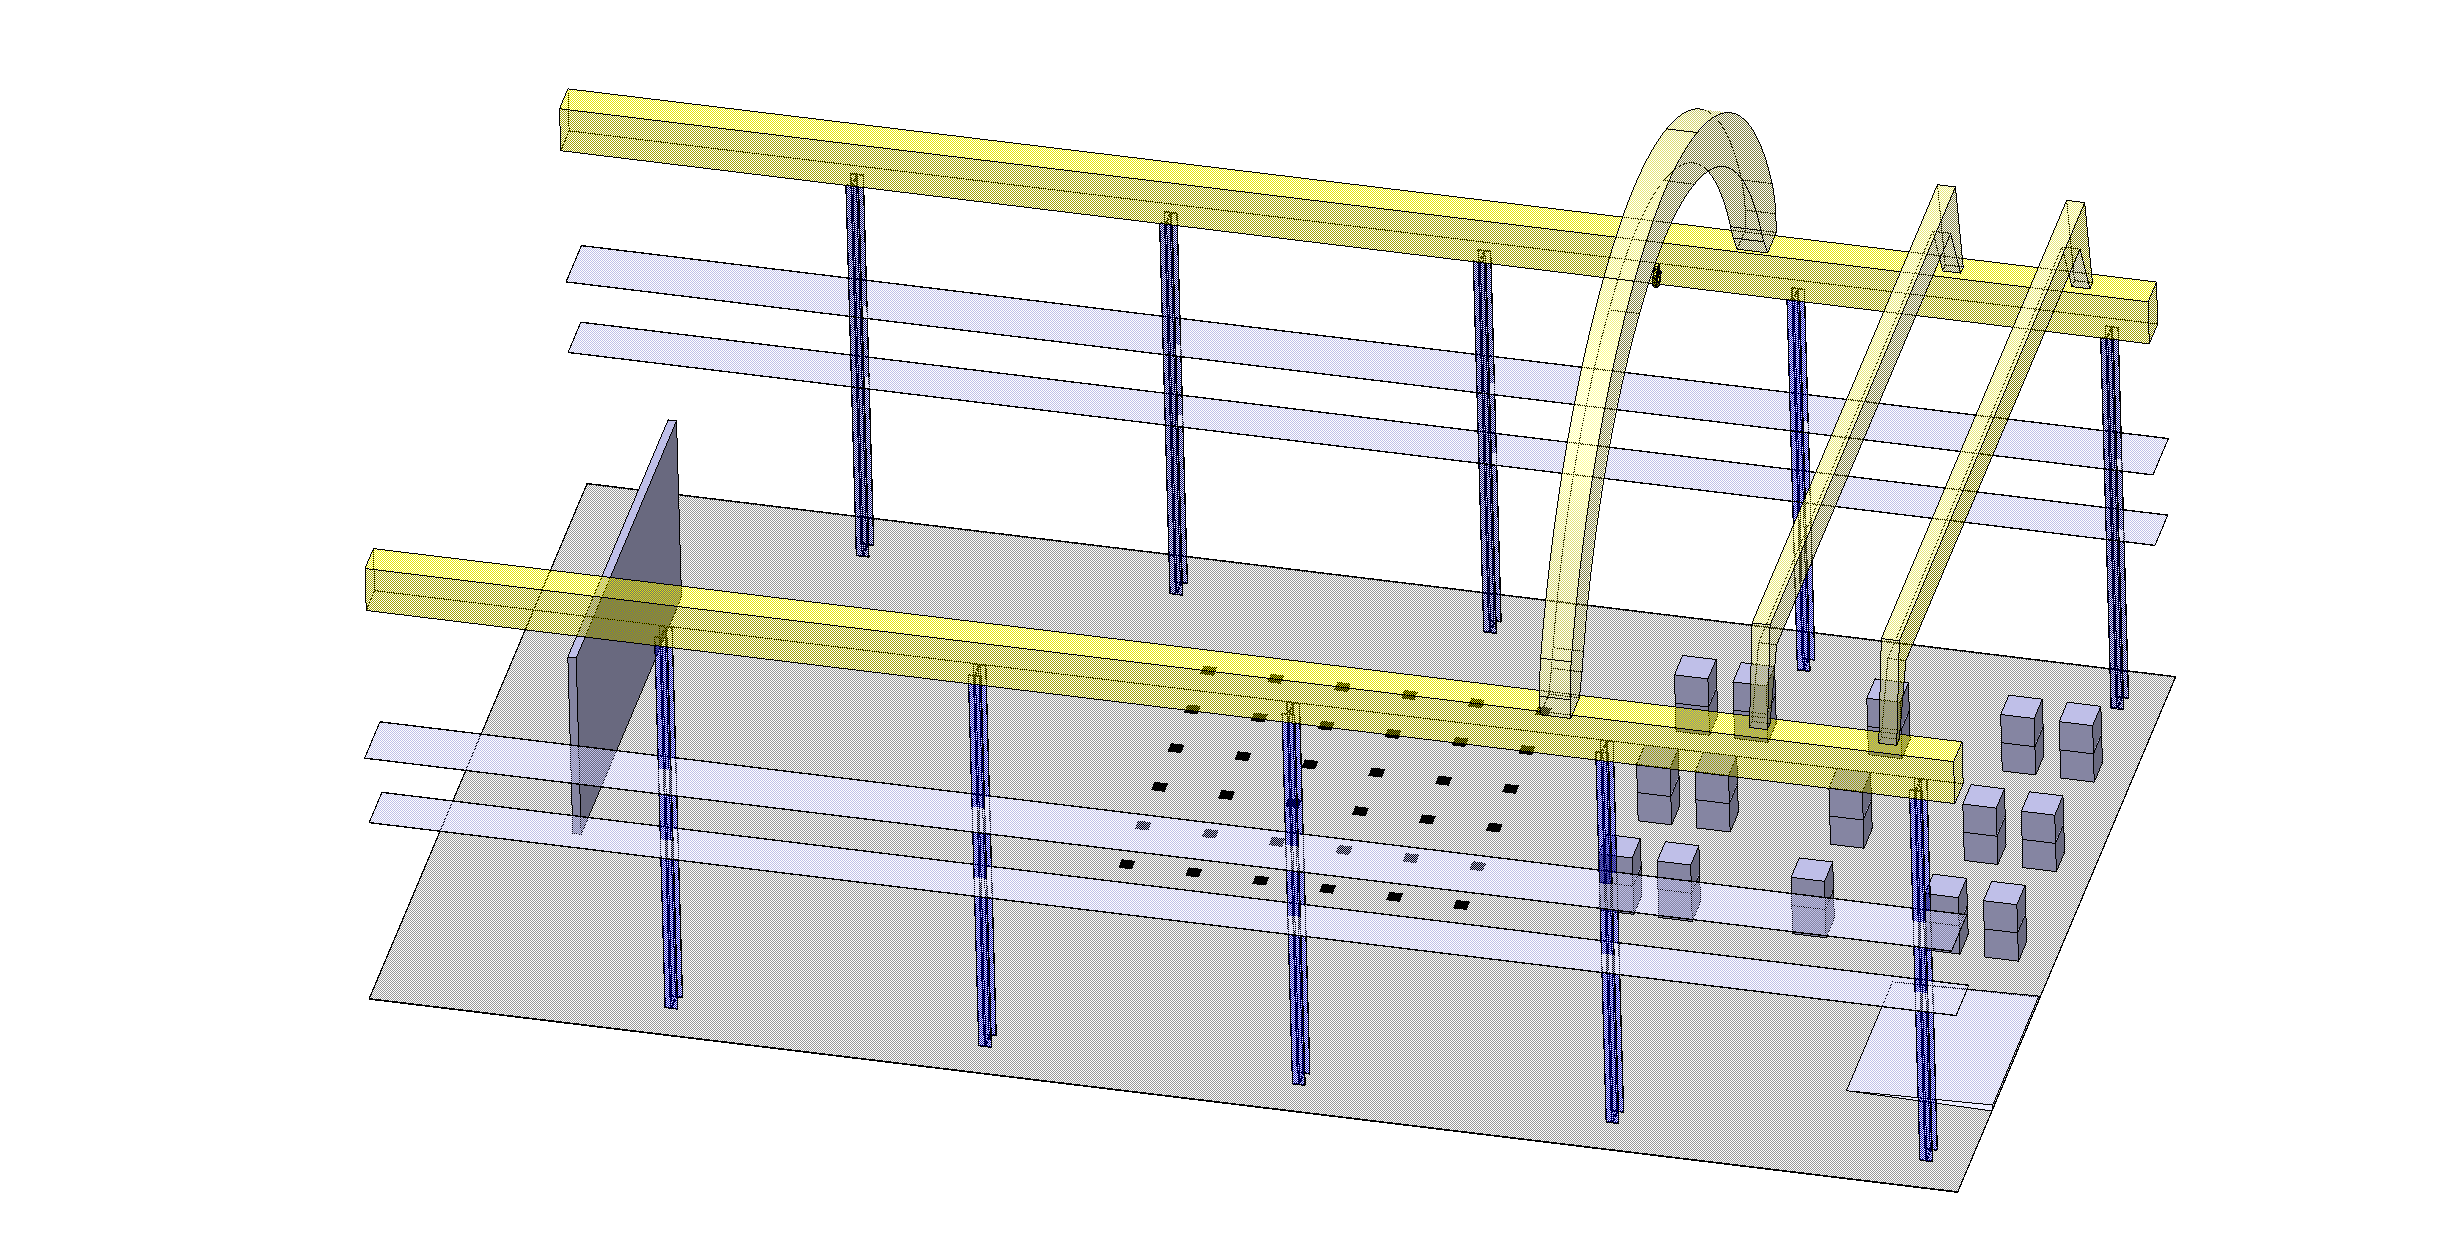
\includegraphics[width=0.32\textwidth]{./Figures/assembly_sequence_11_07/0.png}\label{fig:Ds20kInstallSequence1_a}}
\subfigure[]{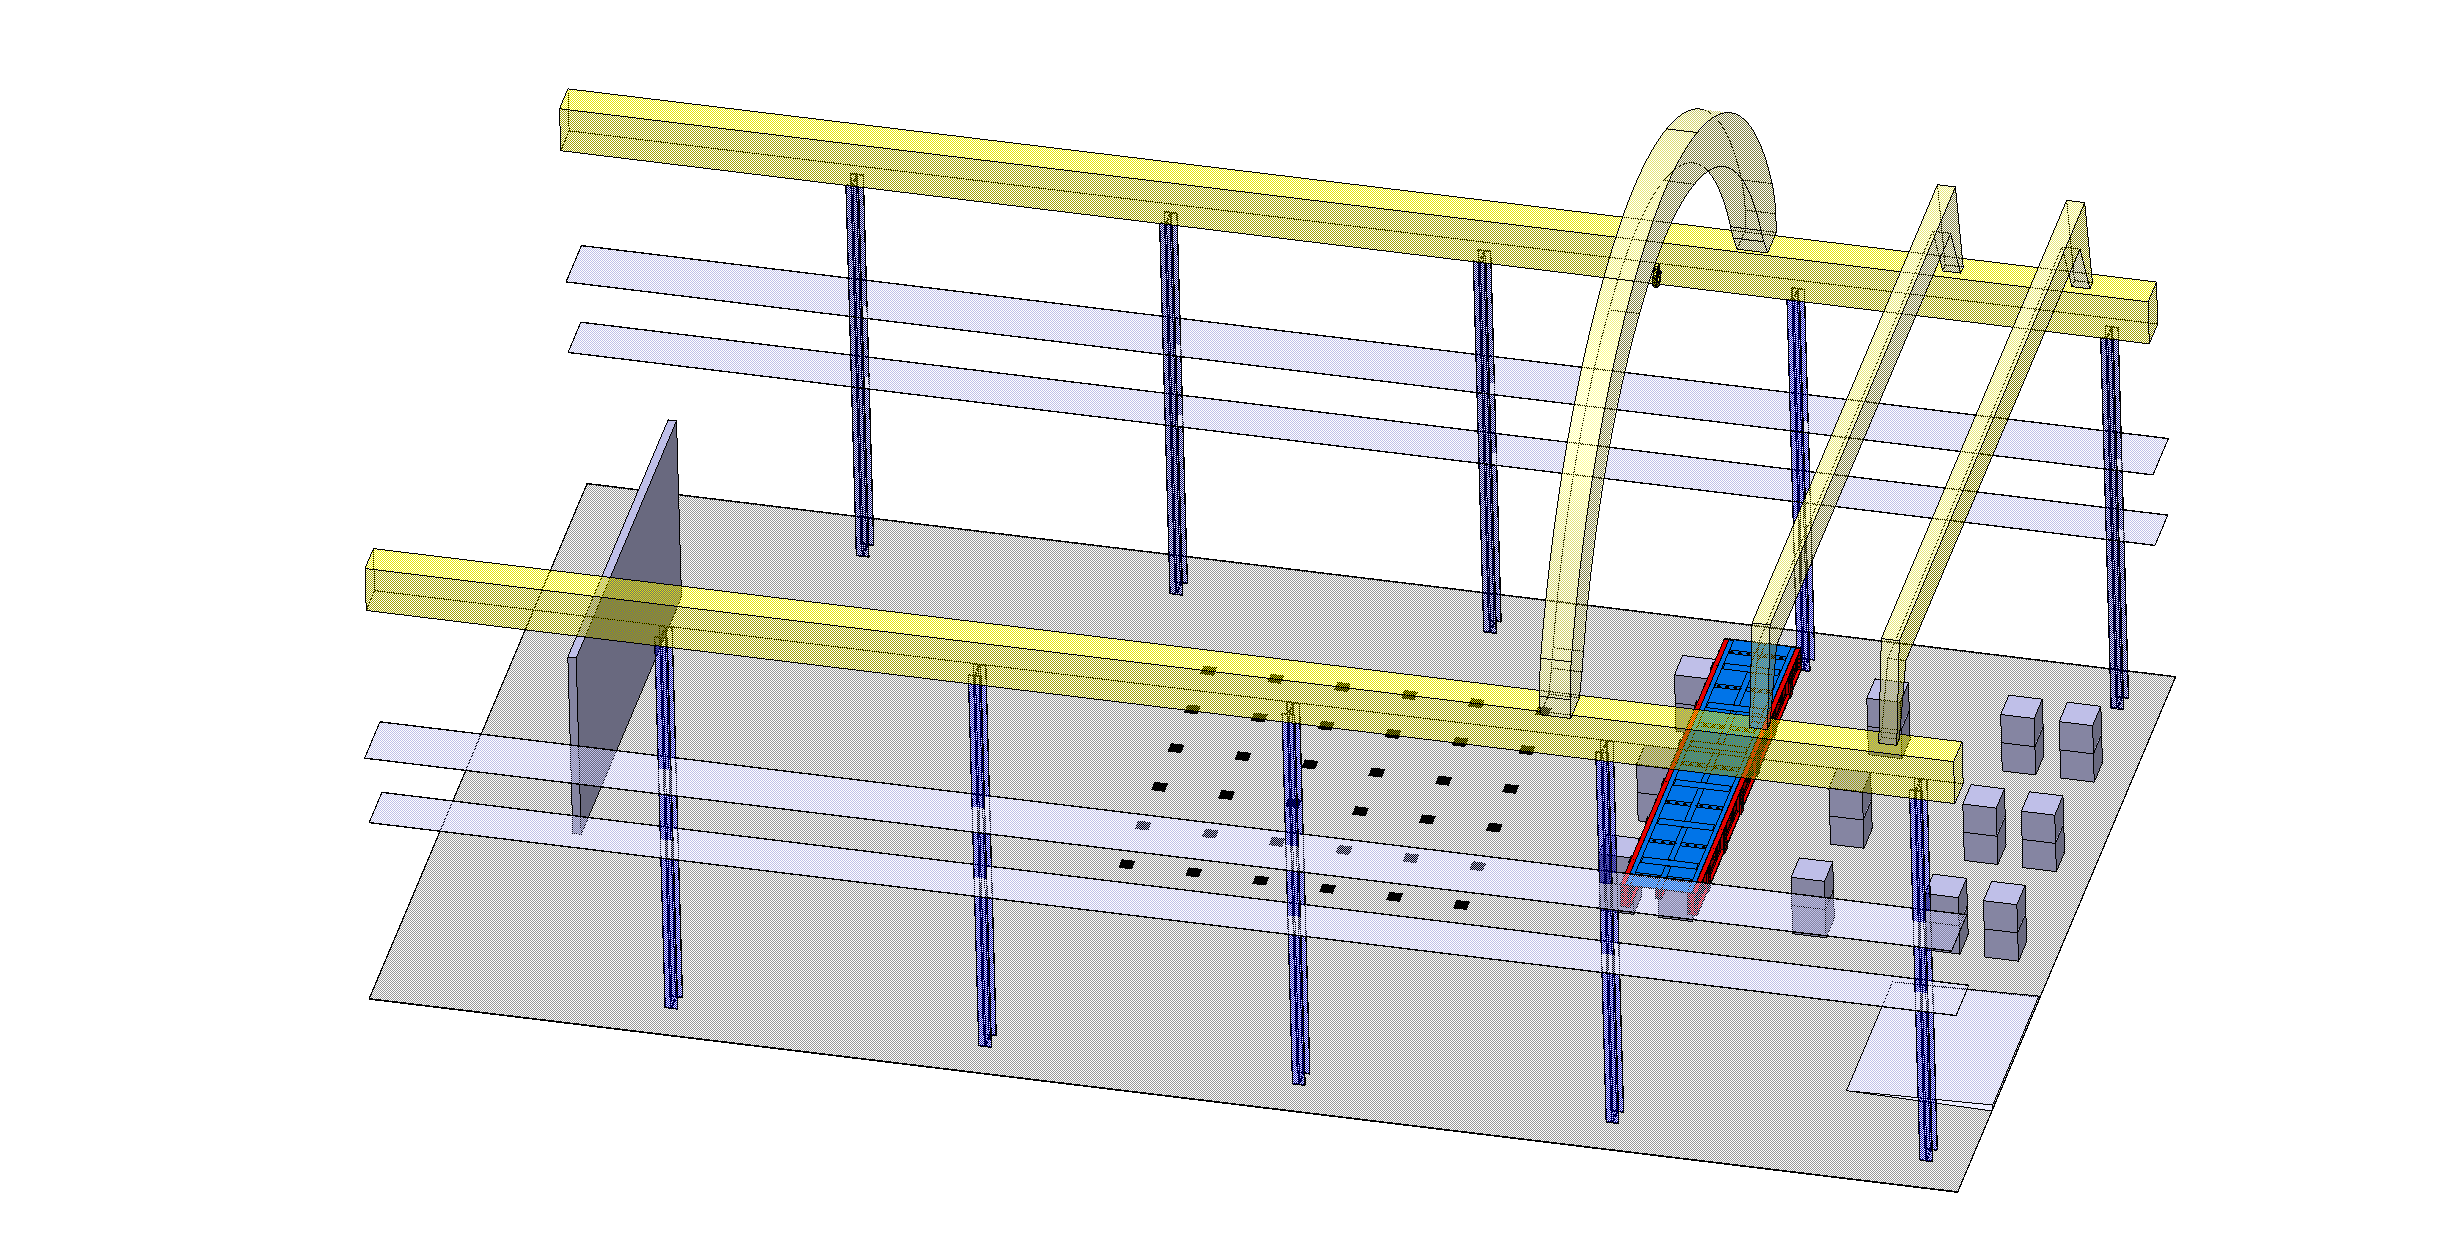
\includegraphics[width=0.32\textwidth]{./Figures/assembly_sequence_11_07/1.png}}
\subfigure[]{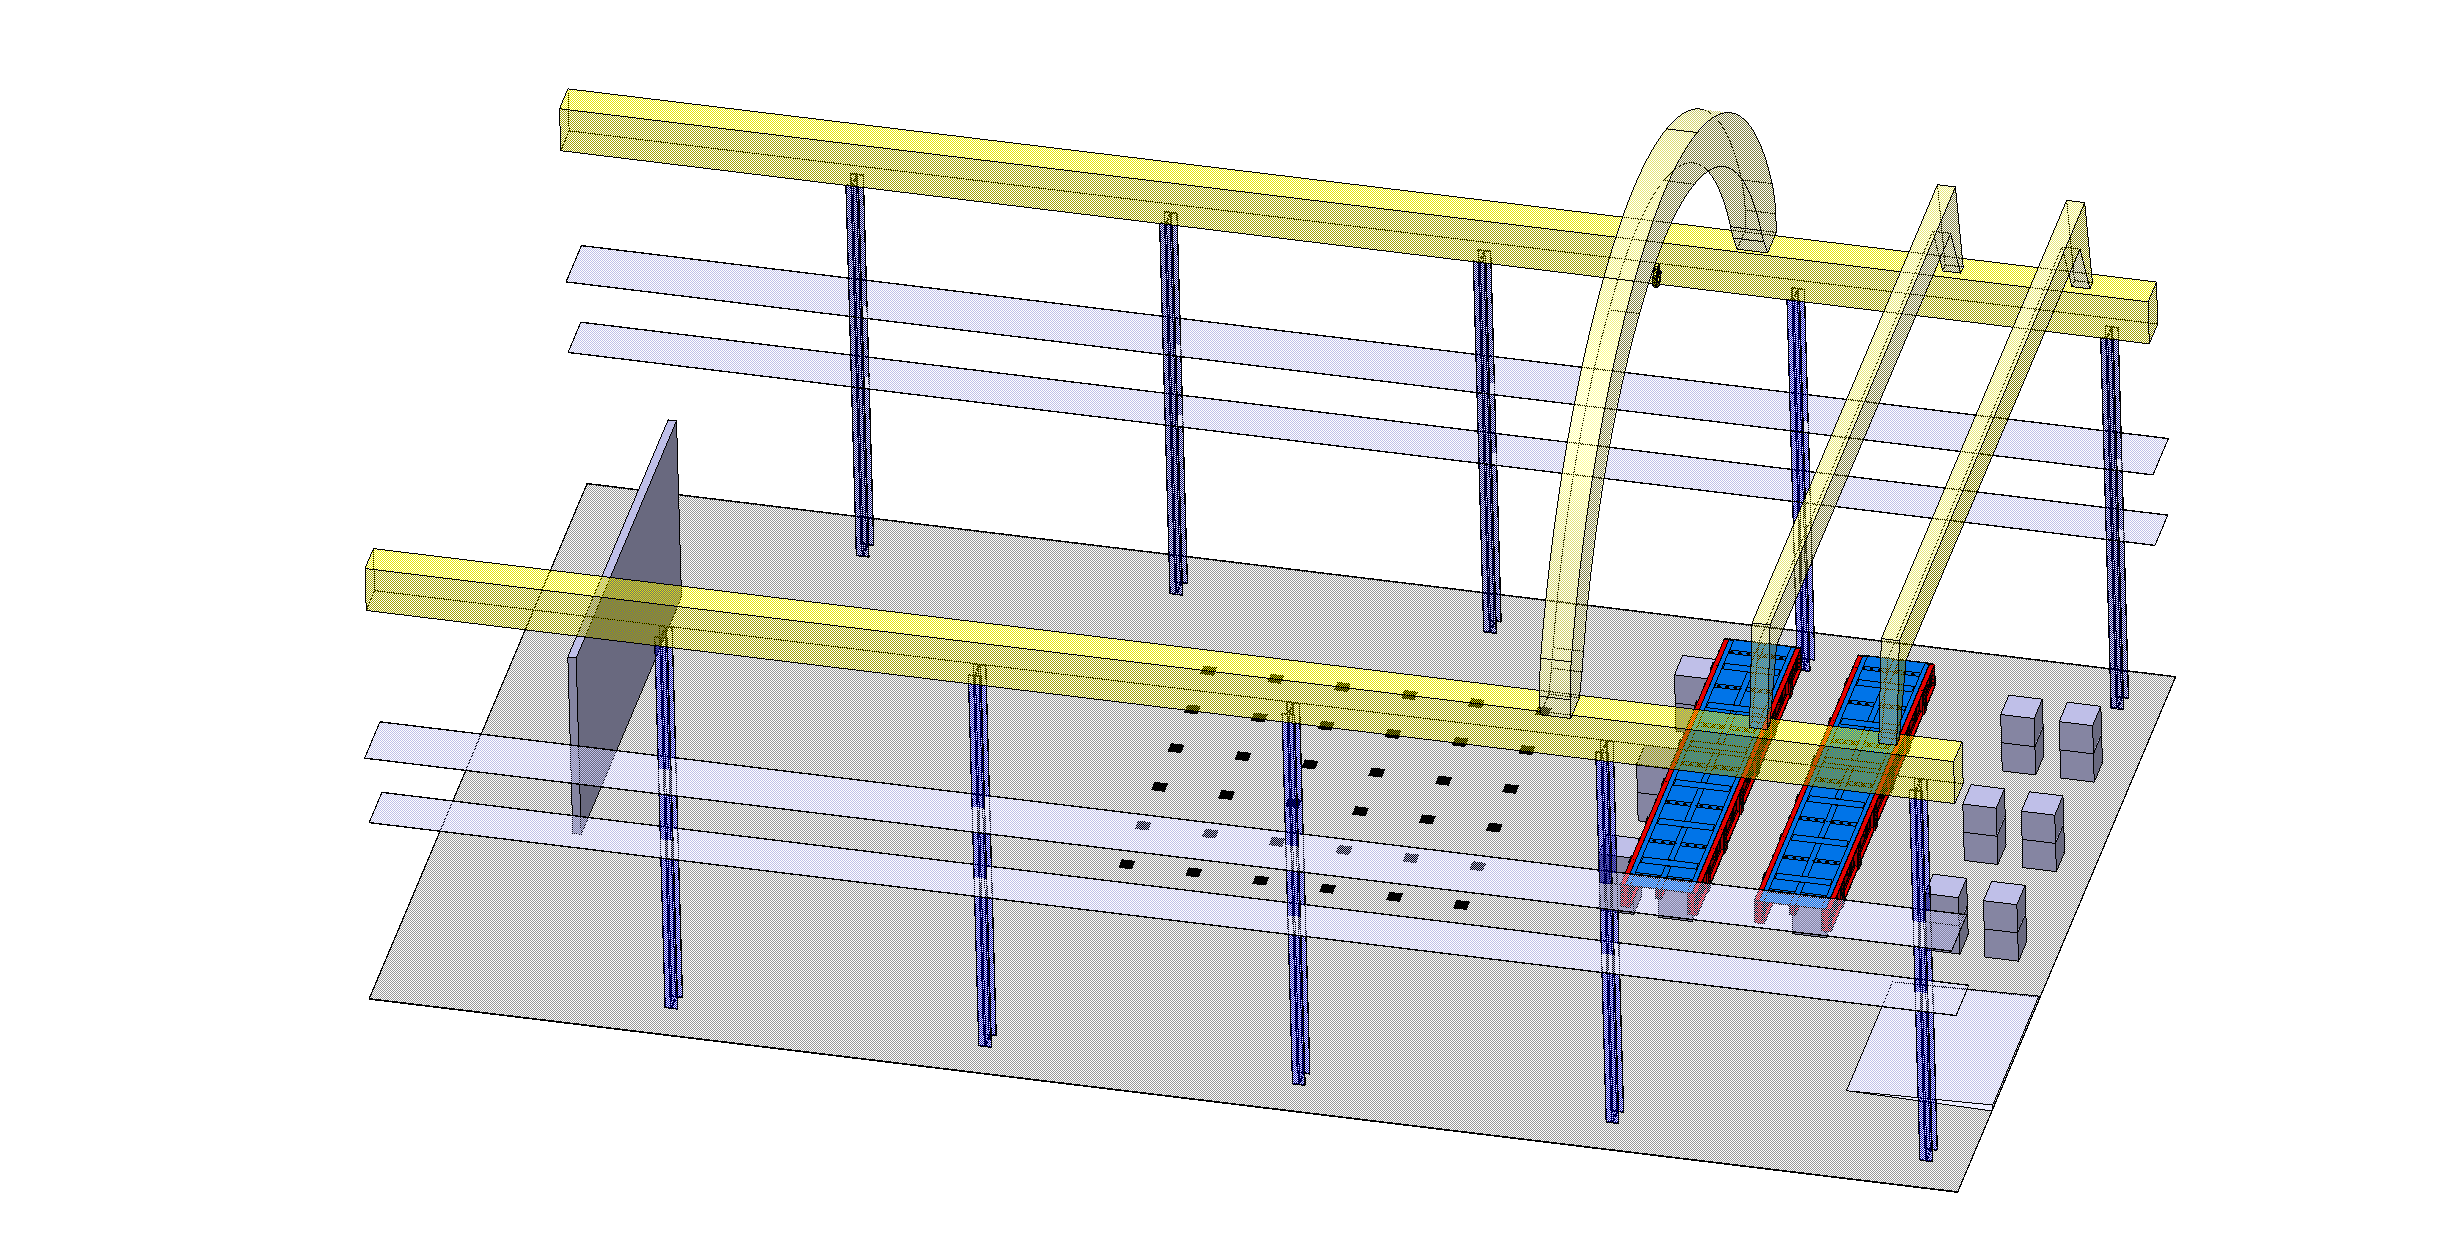
\includegraphics[width=0.32\textwidth]{./Figures/assembly_sequence_11_07/2.png}}
\subfigure[]{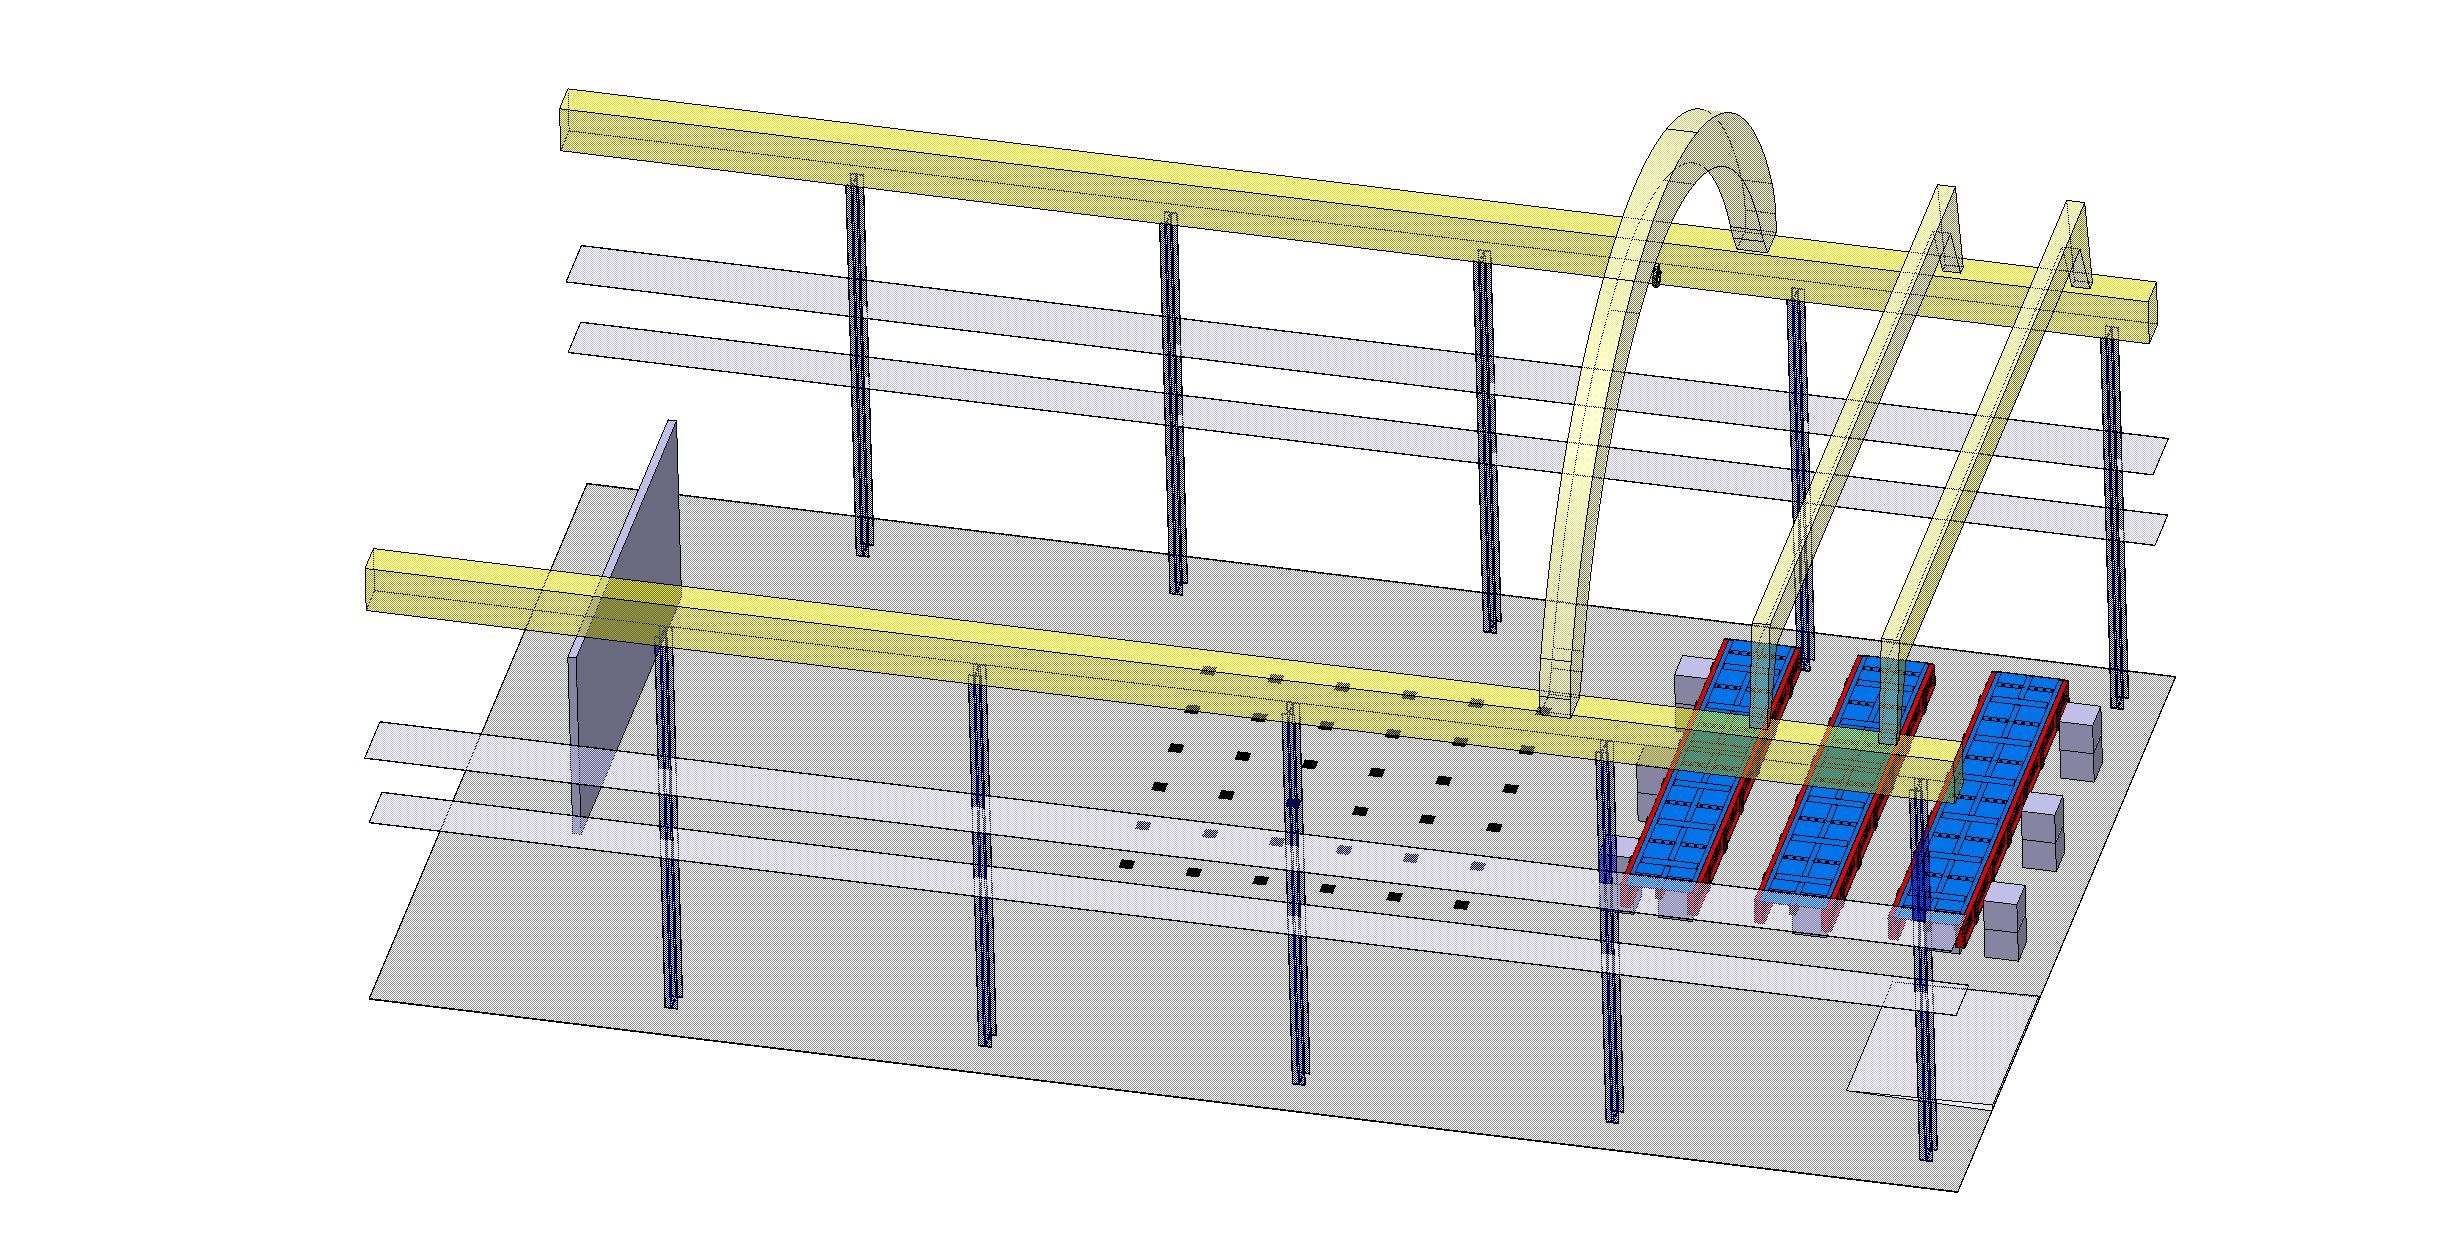
\includegraphics[width=0.32\textwidth]{./Figures/assembly_sequence_11_07/3.png}}
\subfigure[]{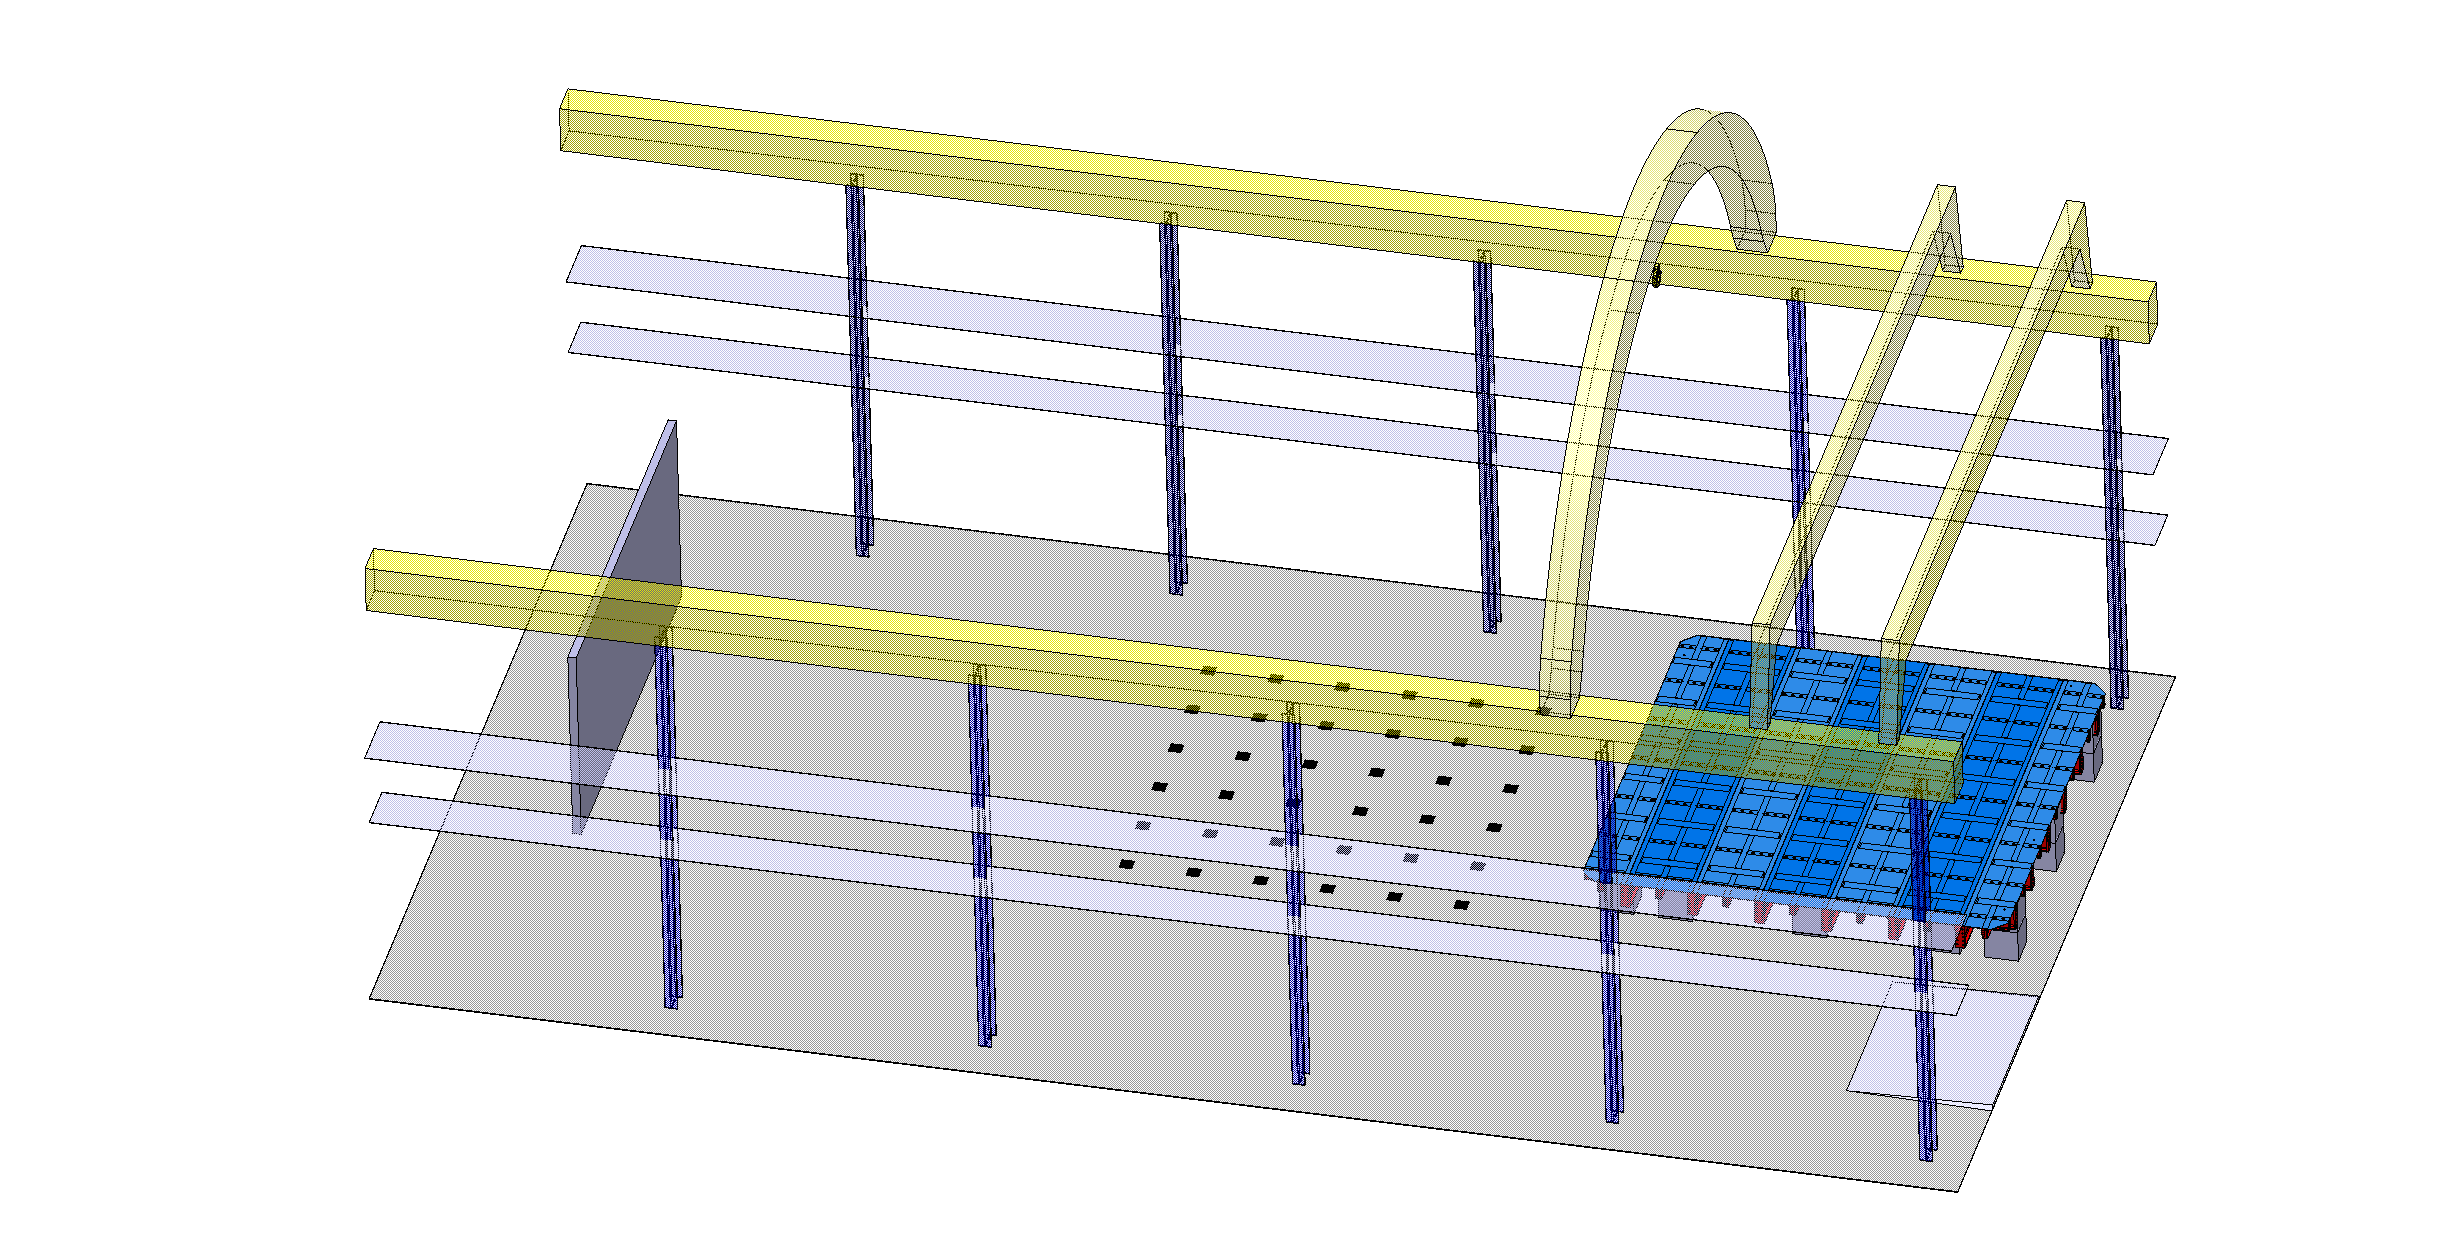
\includegraphics[width=0.32\textwidth]{./Figures/assembly_sequence_11_07/4.png}}
\subfigure[]{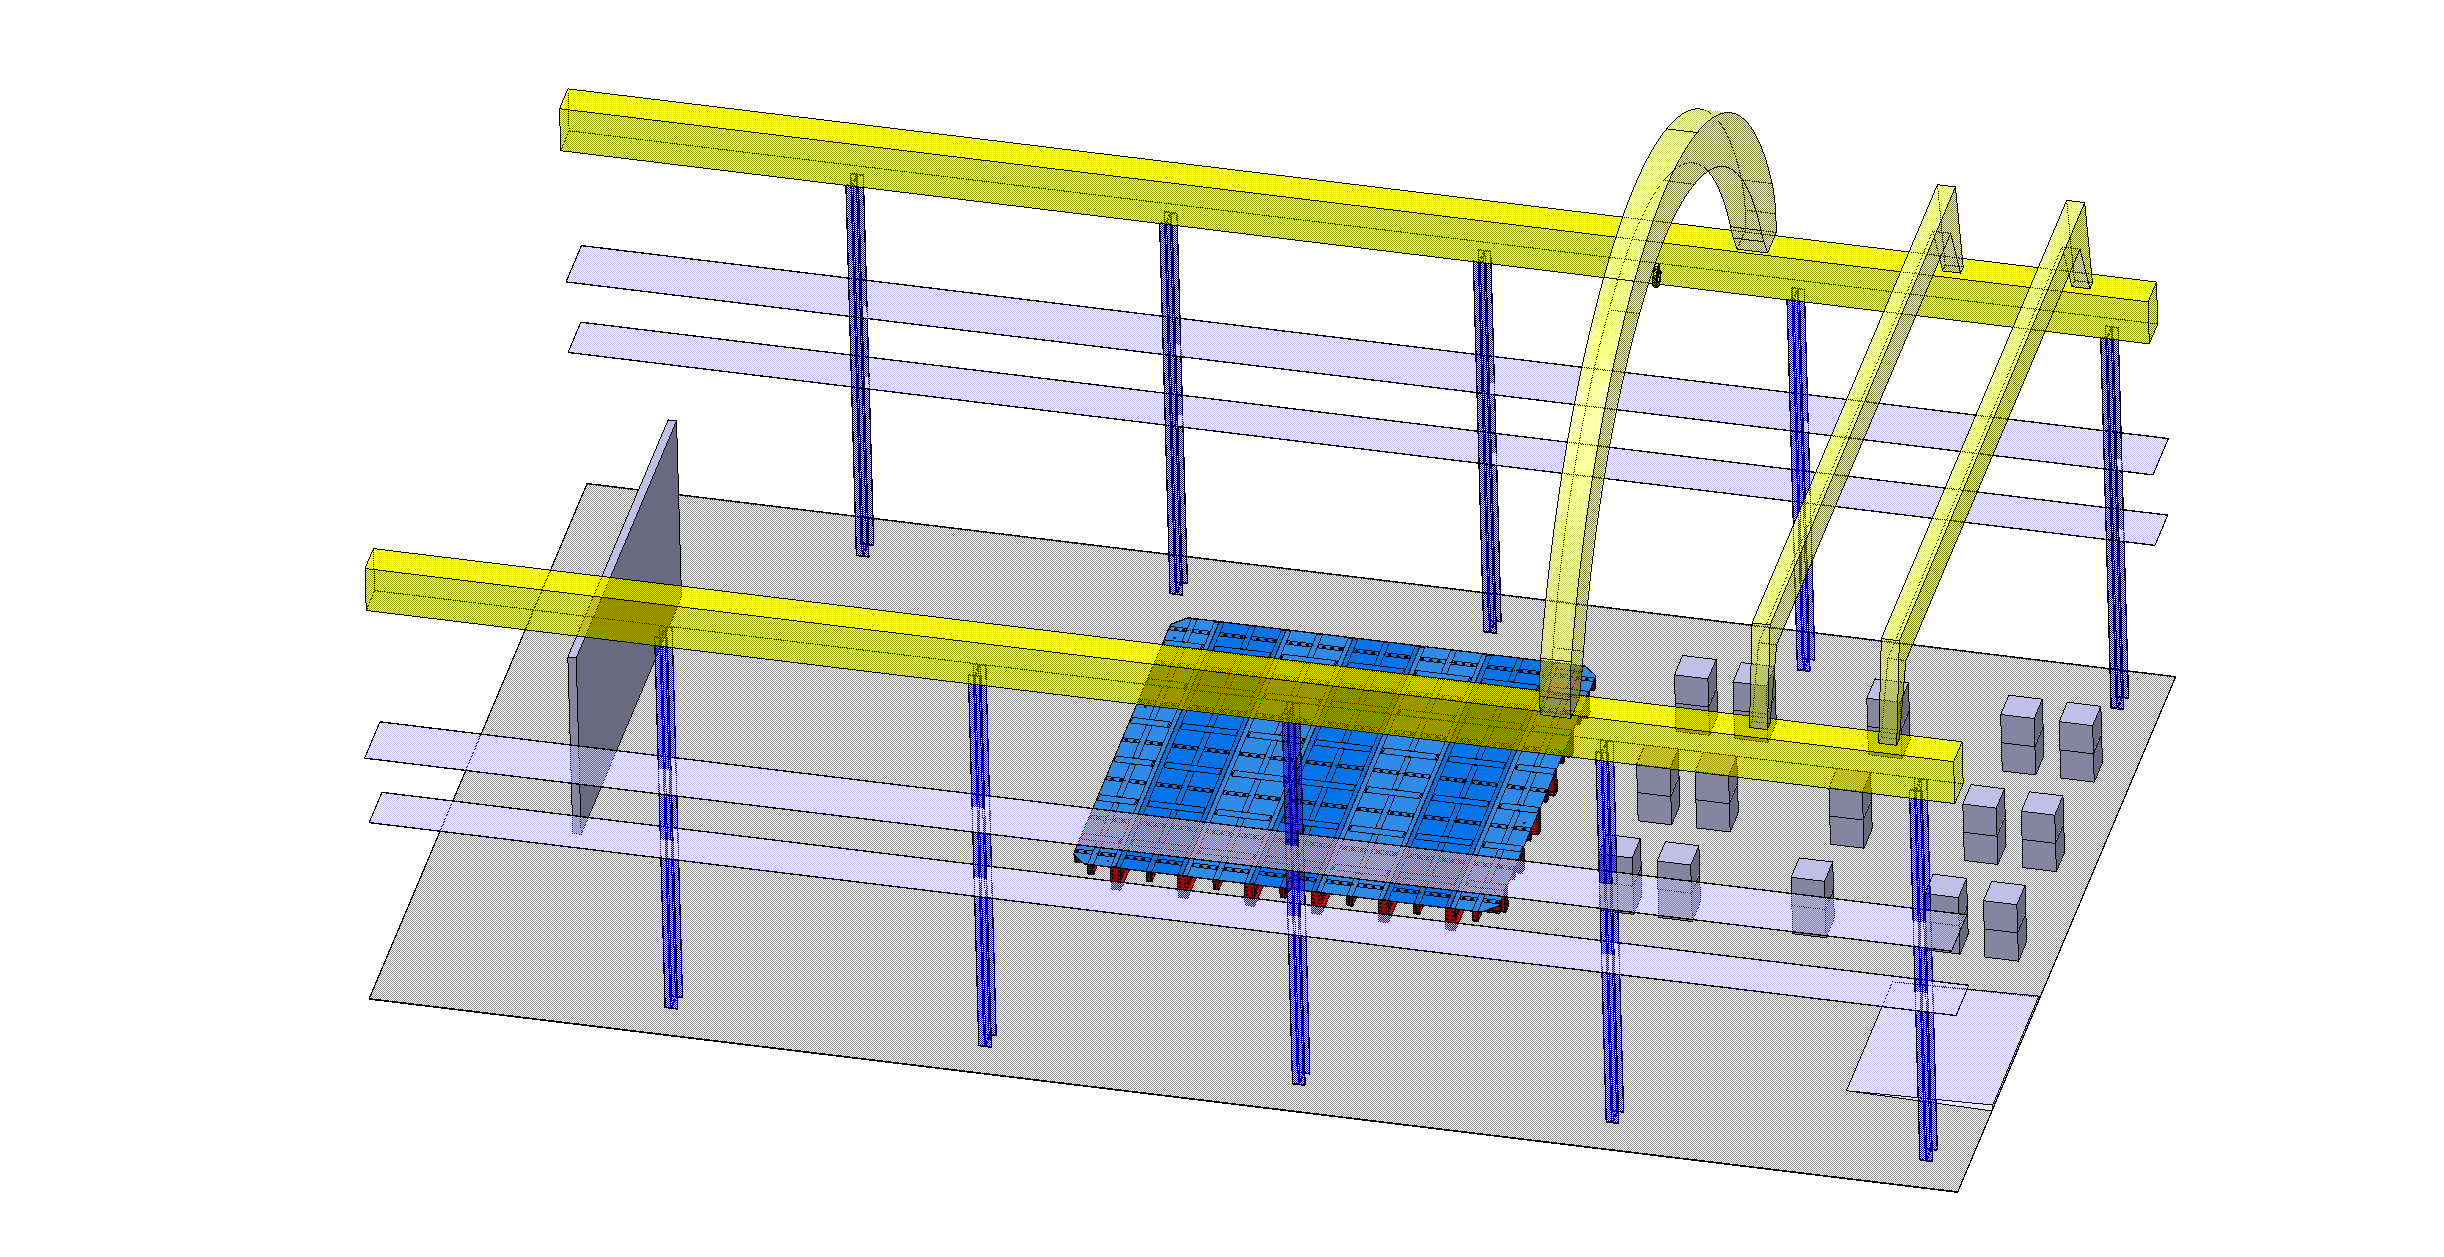
\includegraphics[width=0.32\textwidth]{./Figures/assembly_sequence_11_07/5.png}}
\subfigure[]{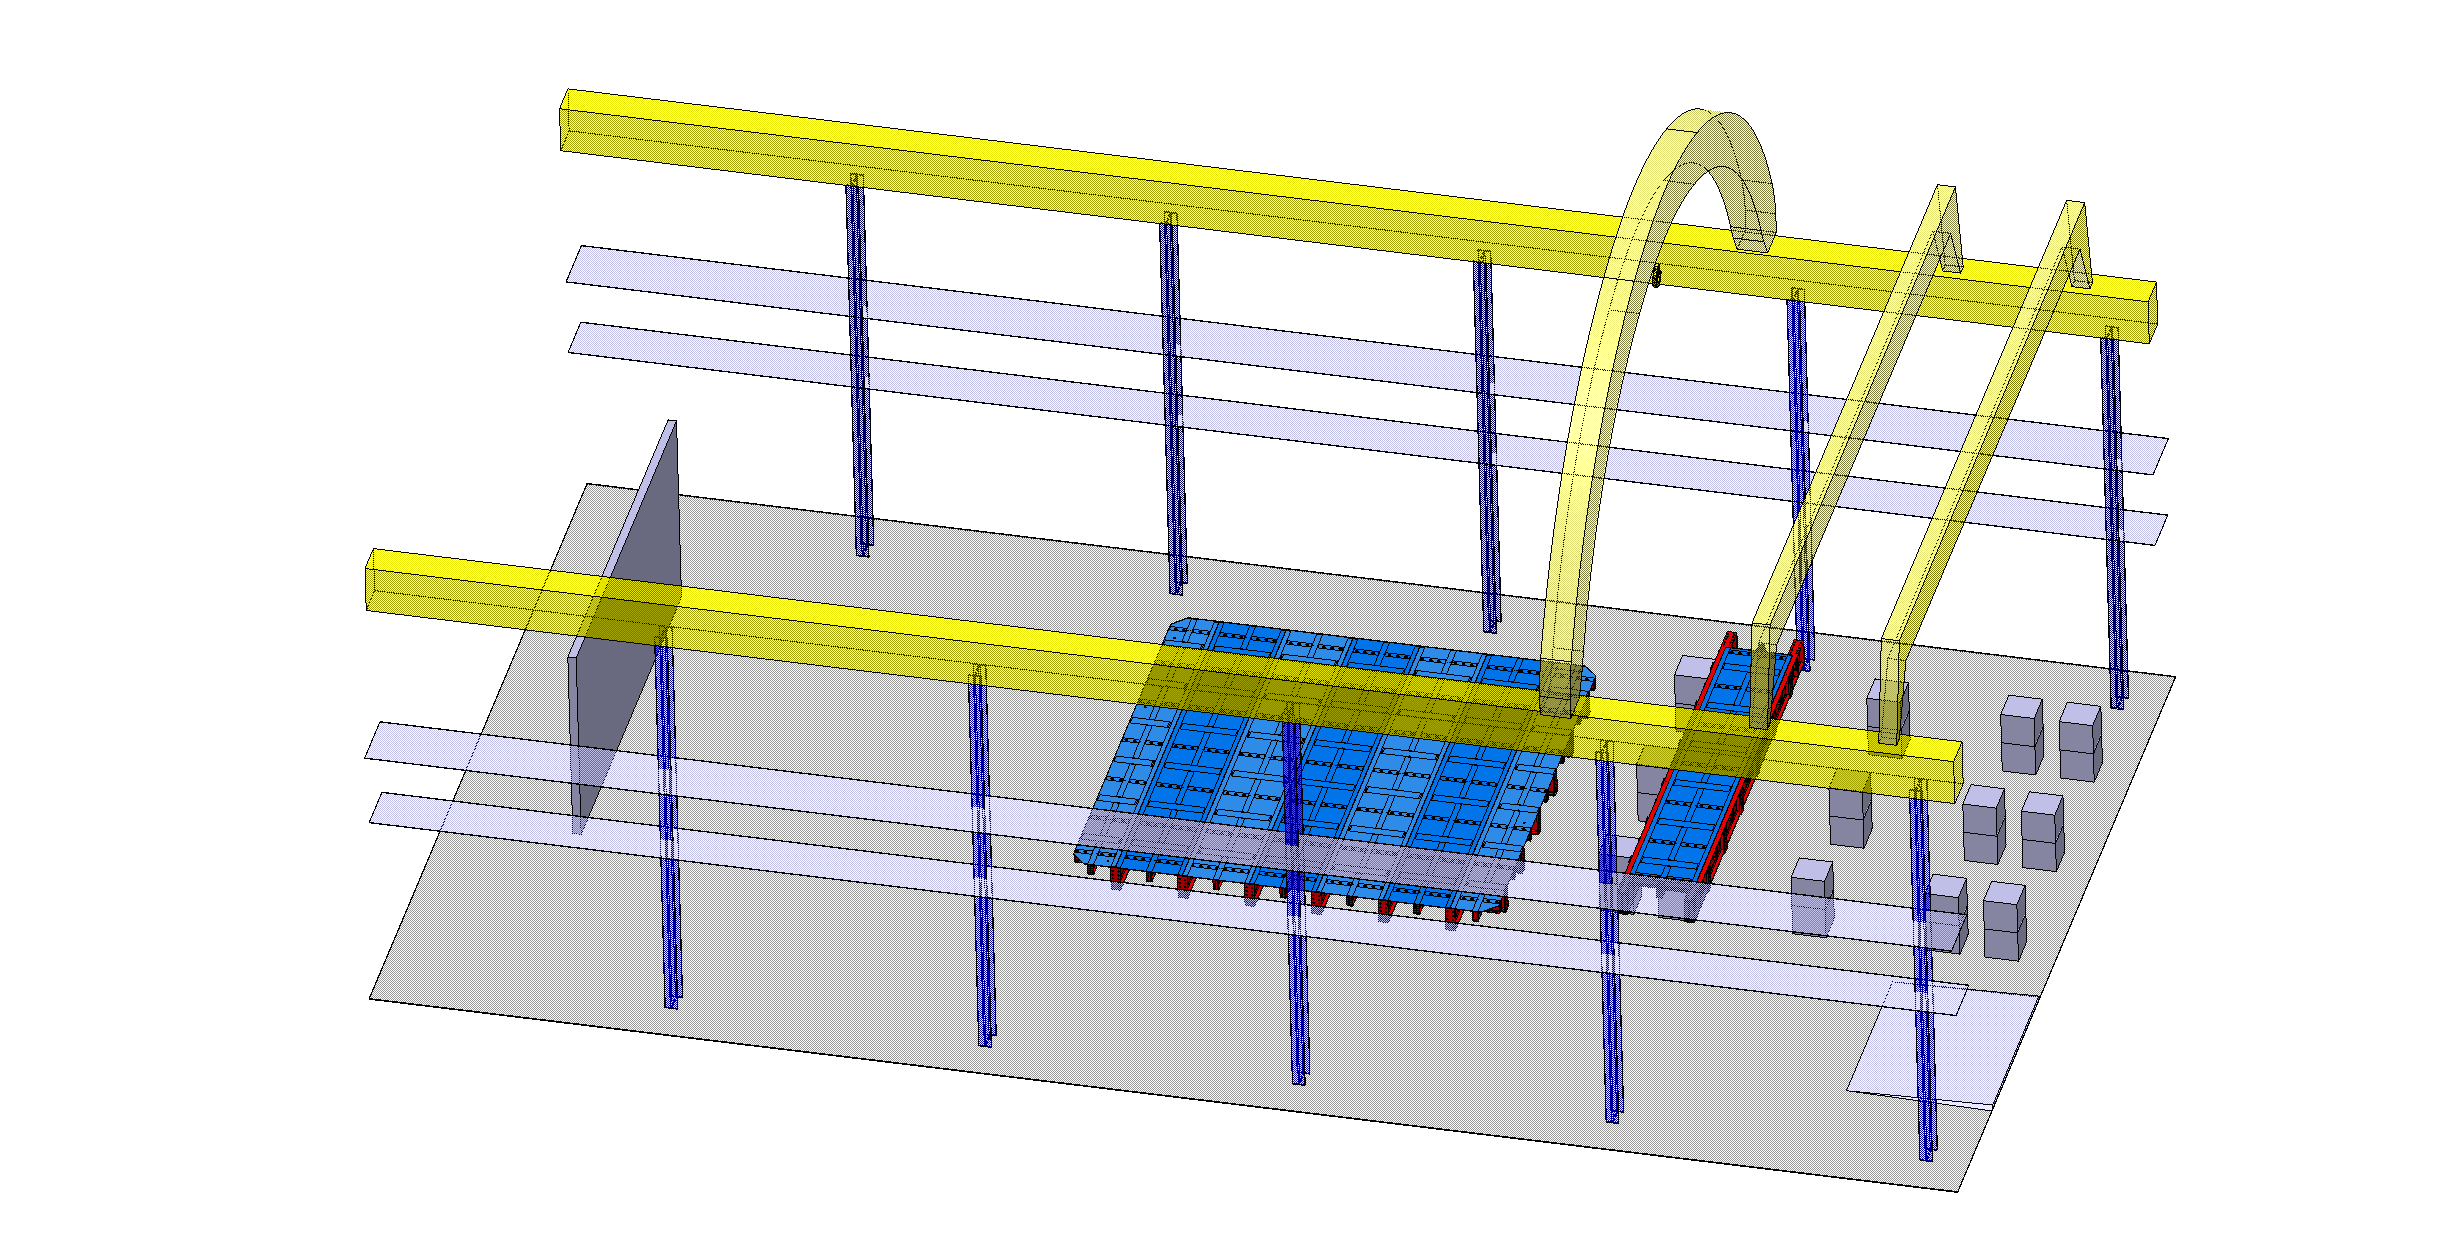
\includegraphics[width=0.32\textwidth]{./Figures/assembly_sequence_11_07/6.png}}
\subfigure[]{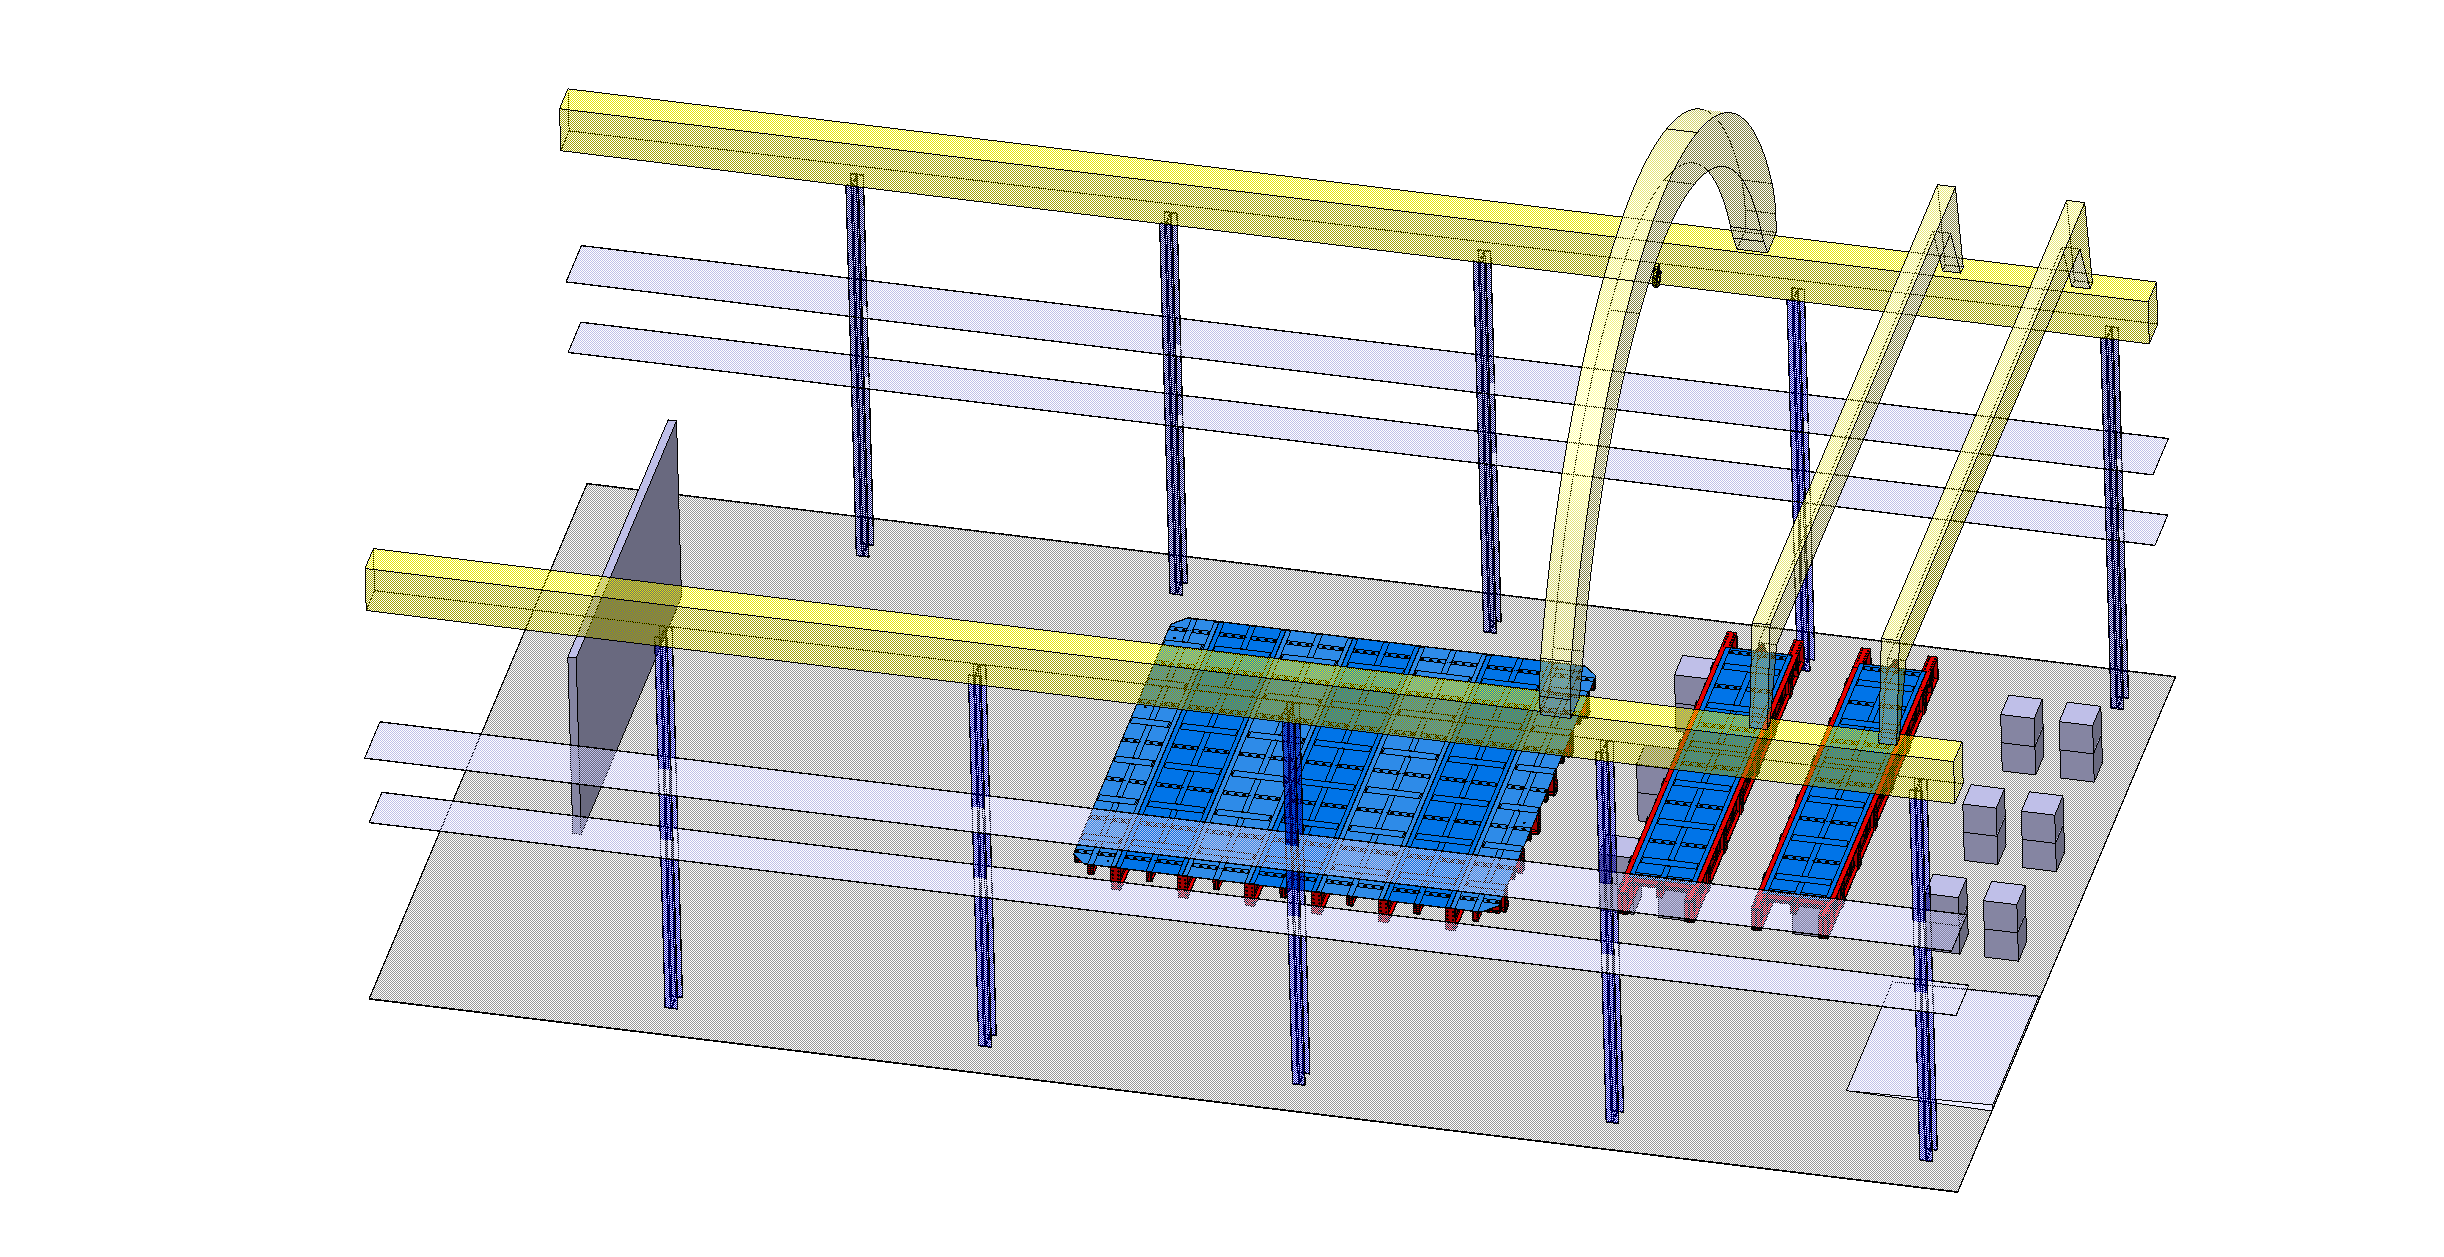
\includegraphics[width=0.32\textwidth]{./Figures/assembly_sequence_11_07/7.png}}
\subfigure[]{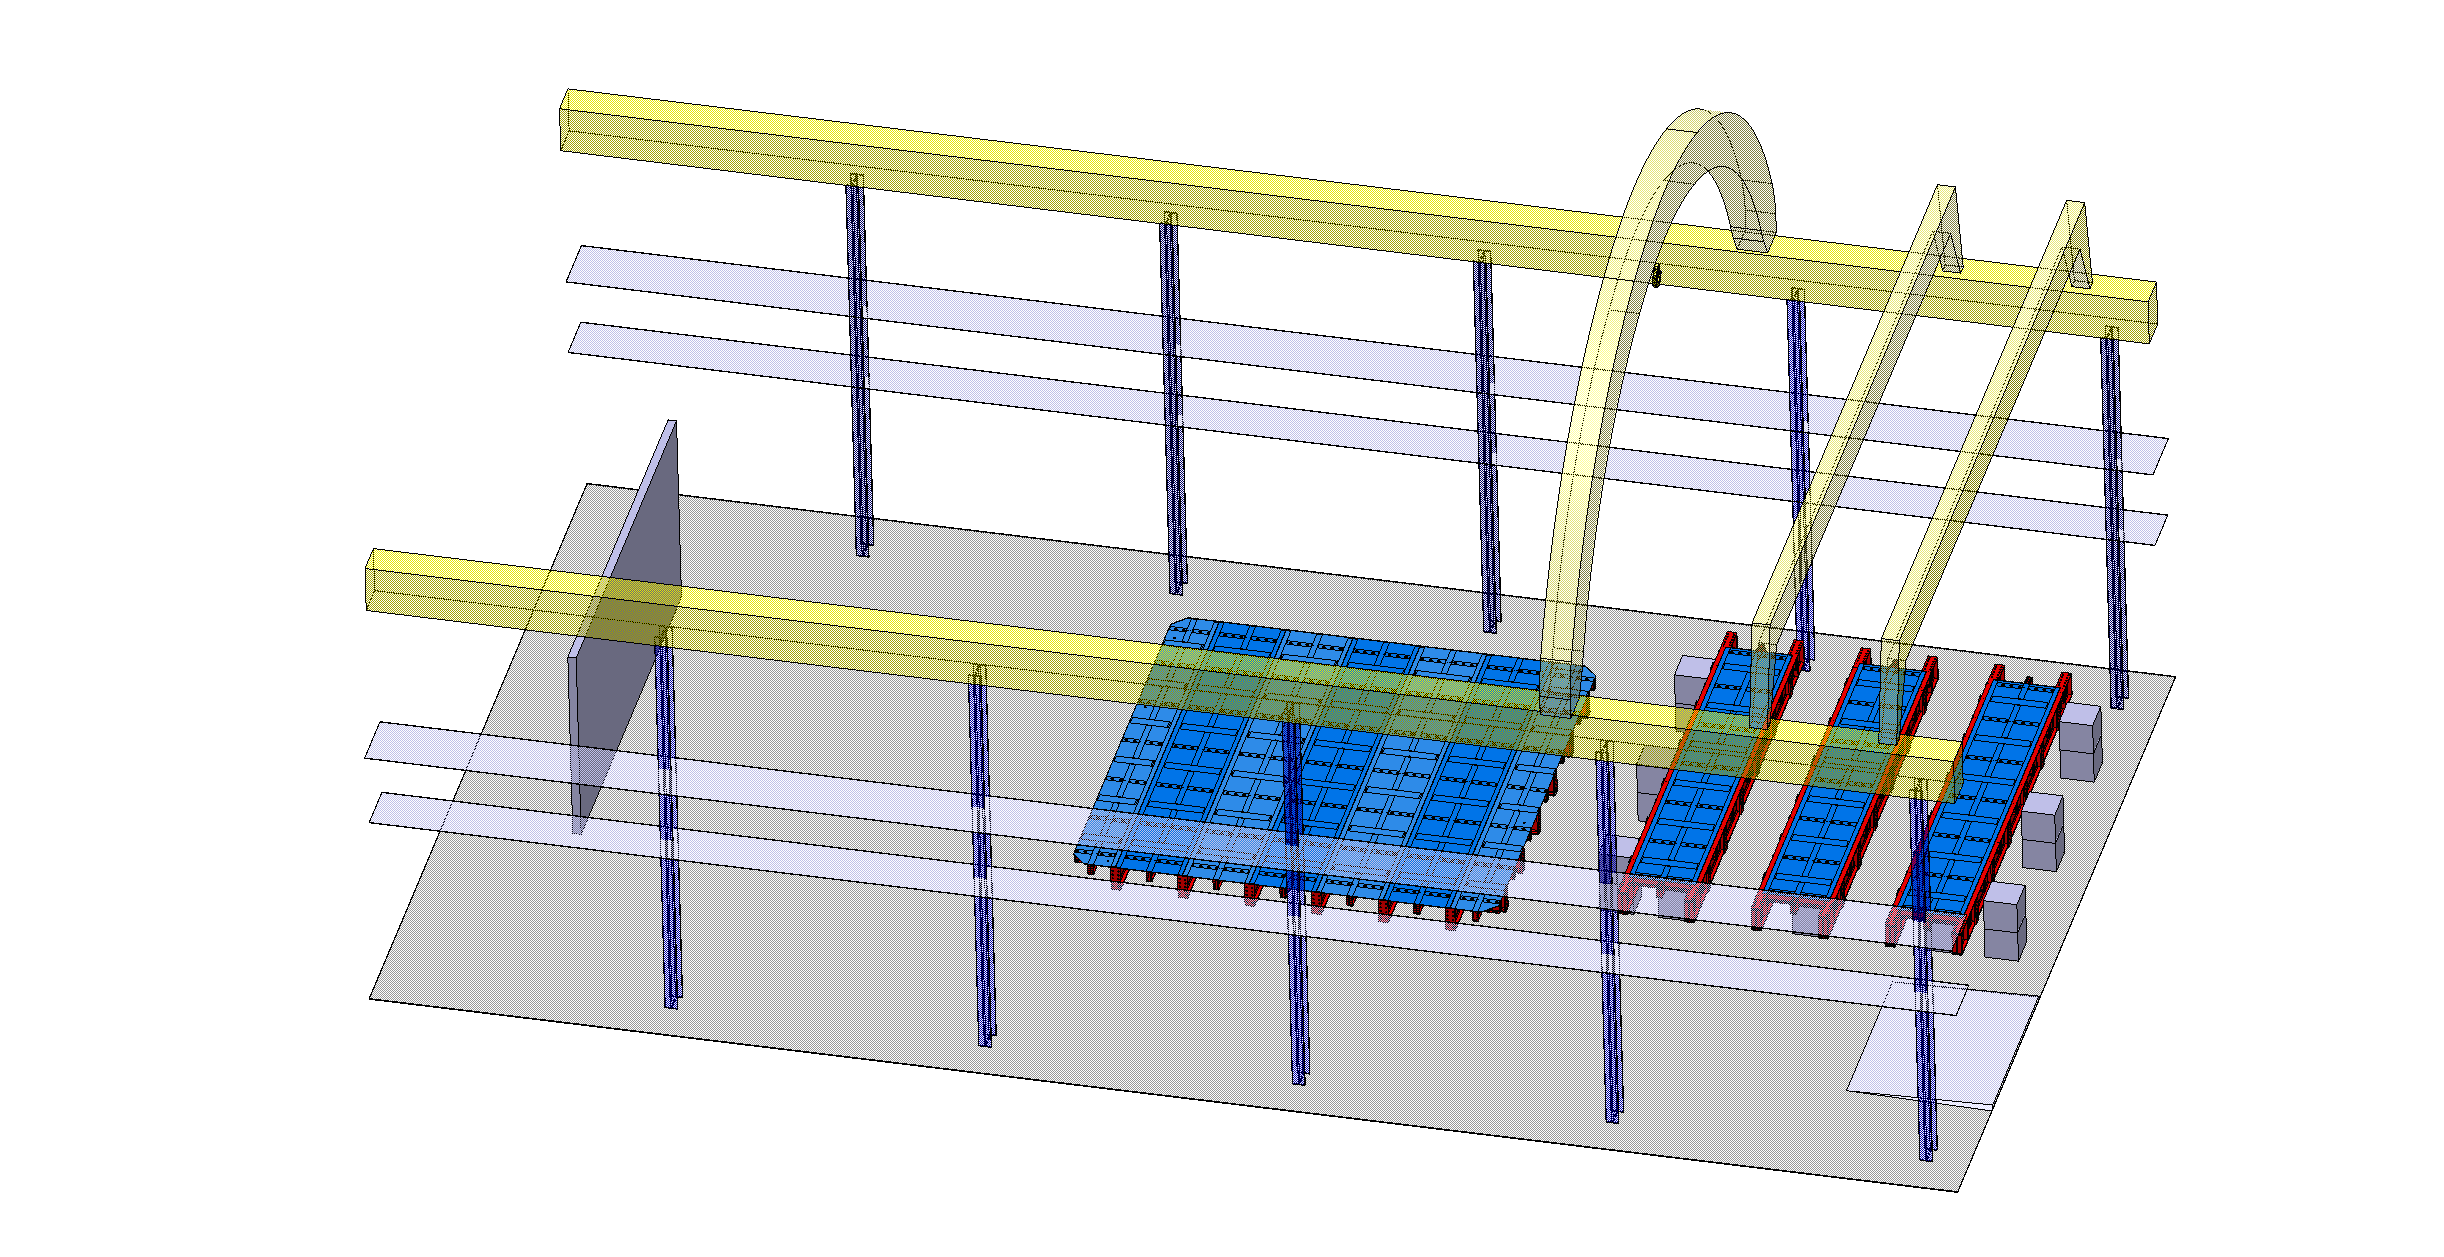
\includegraphics[width=0.32\textwidth]{./Figures/assembly_sequence_11_07/8.png}}
\subfigure[]{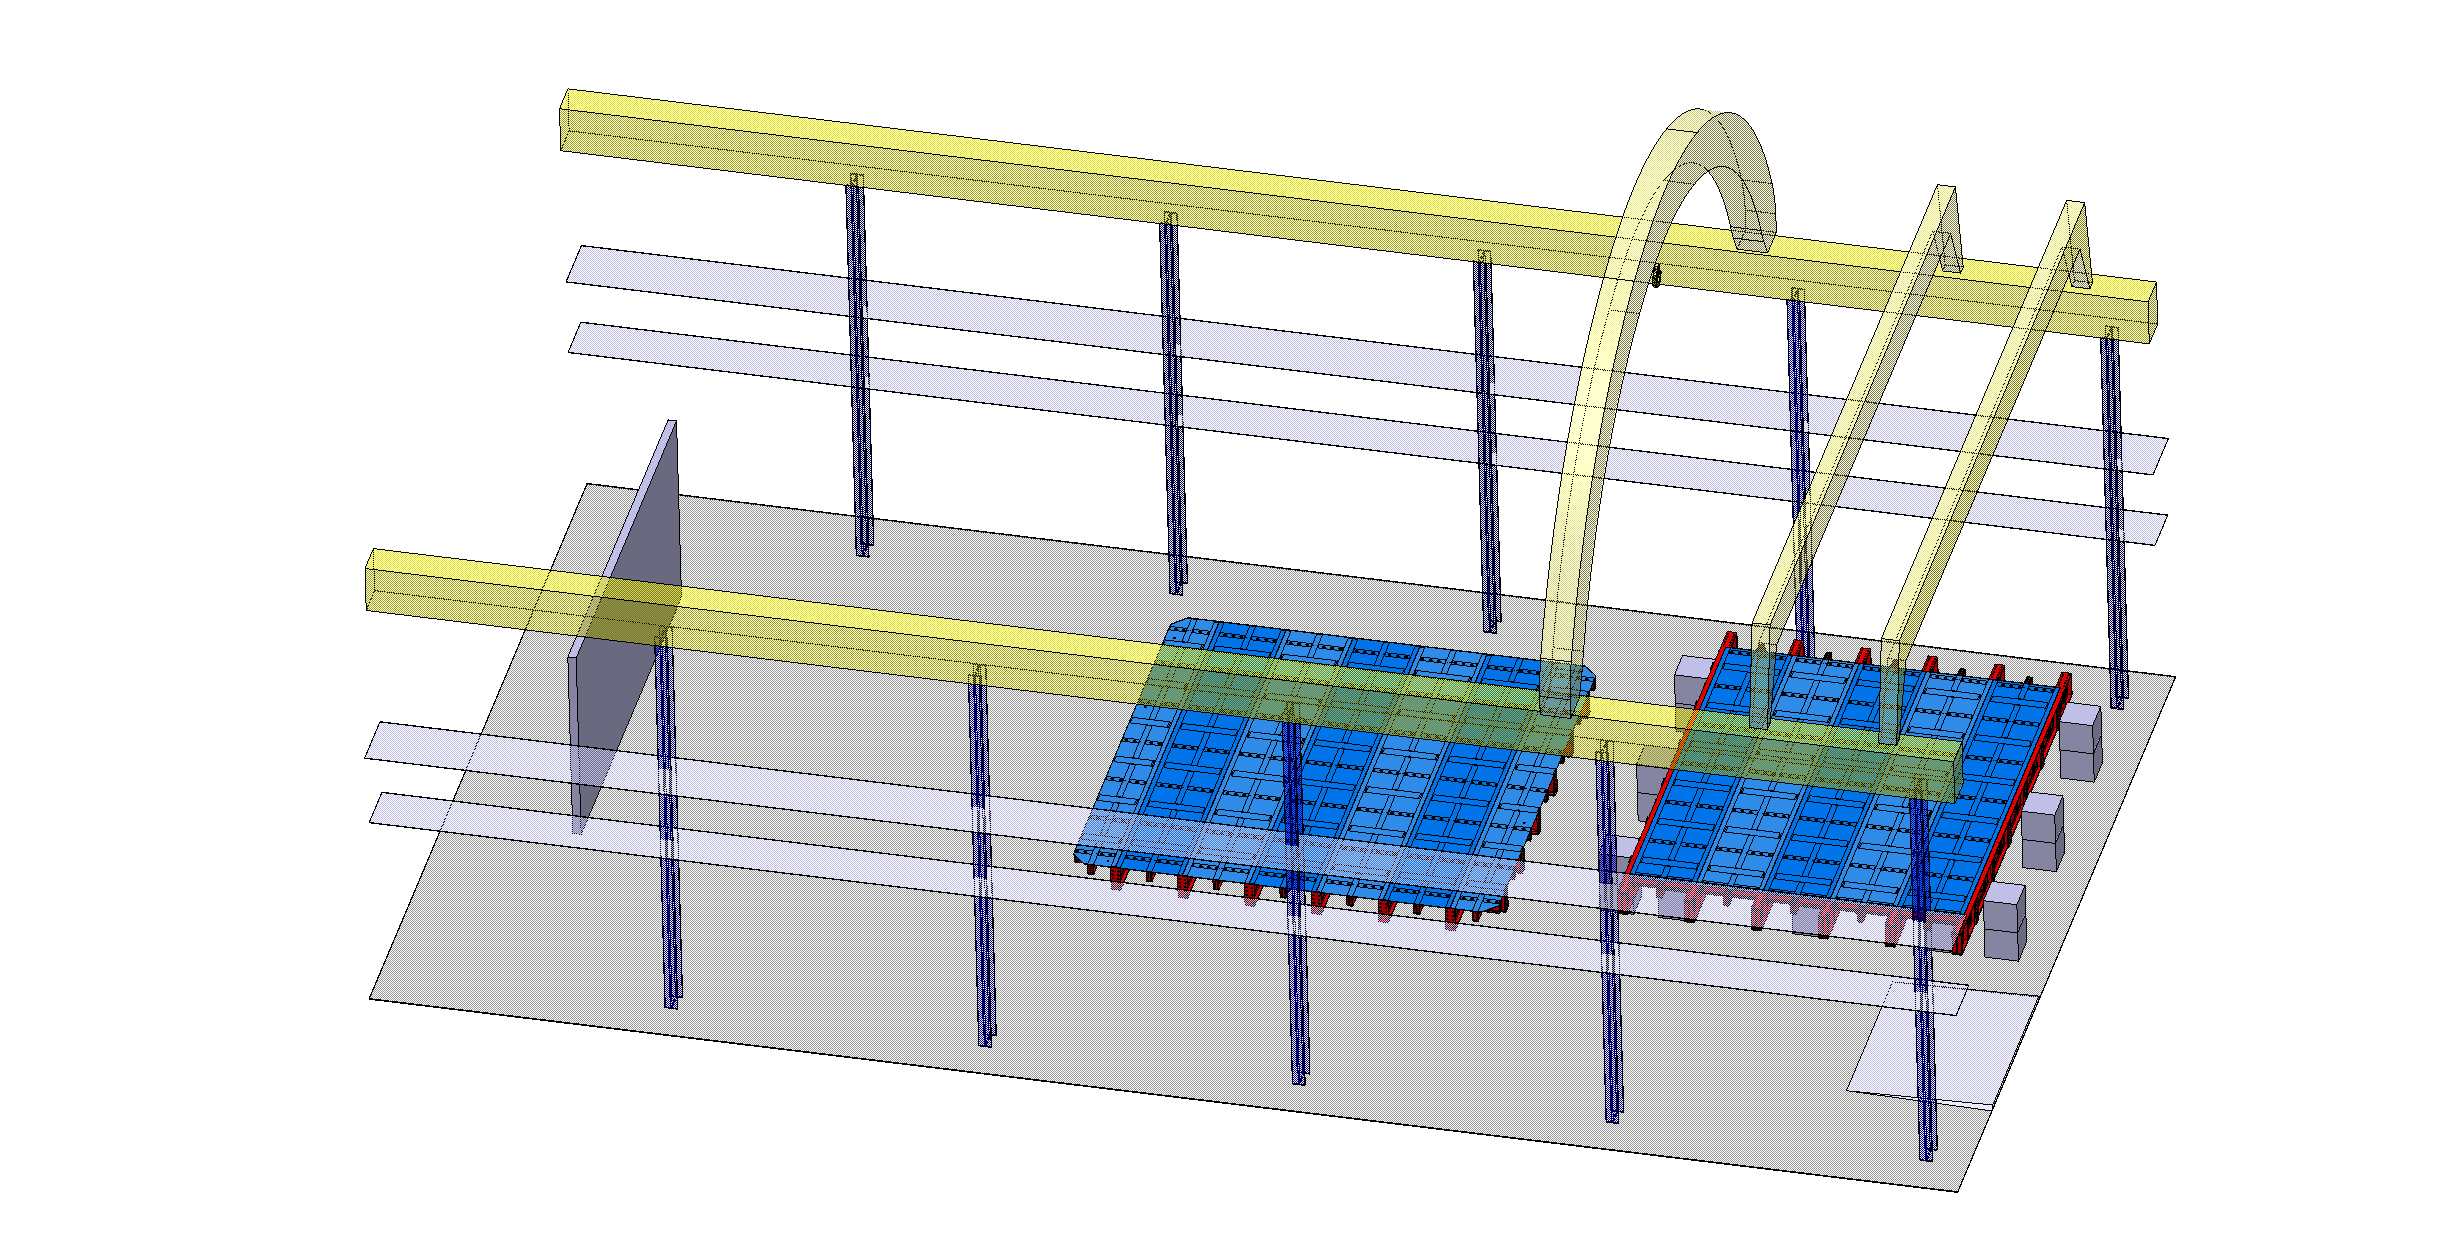
\includegraphics[width=0.32\textwidth]{./Figures/assembly_sequence_11_07/9.png}}
\subfigure[]{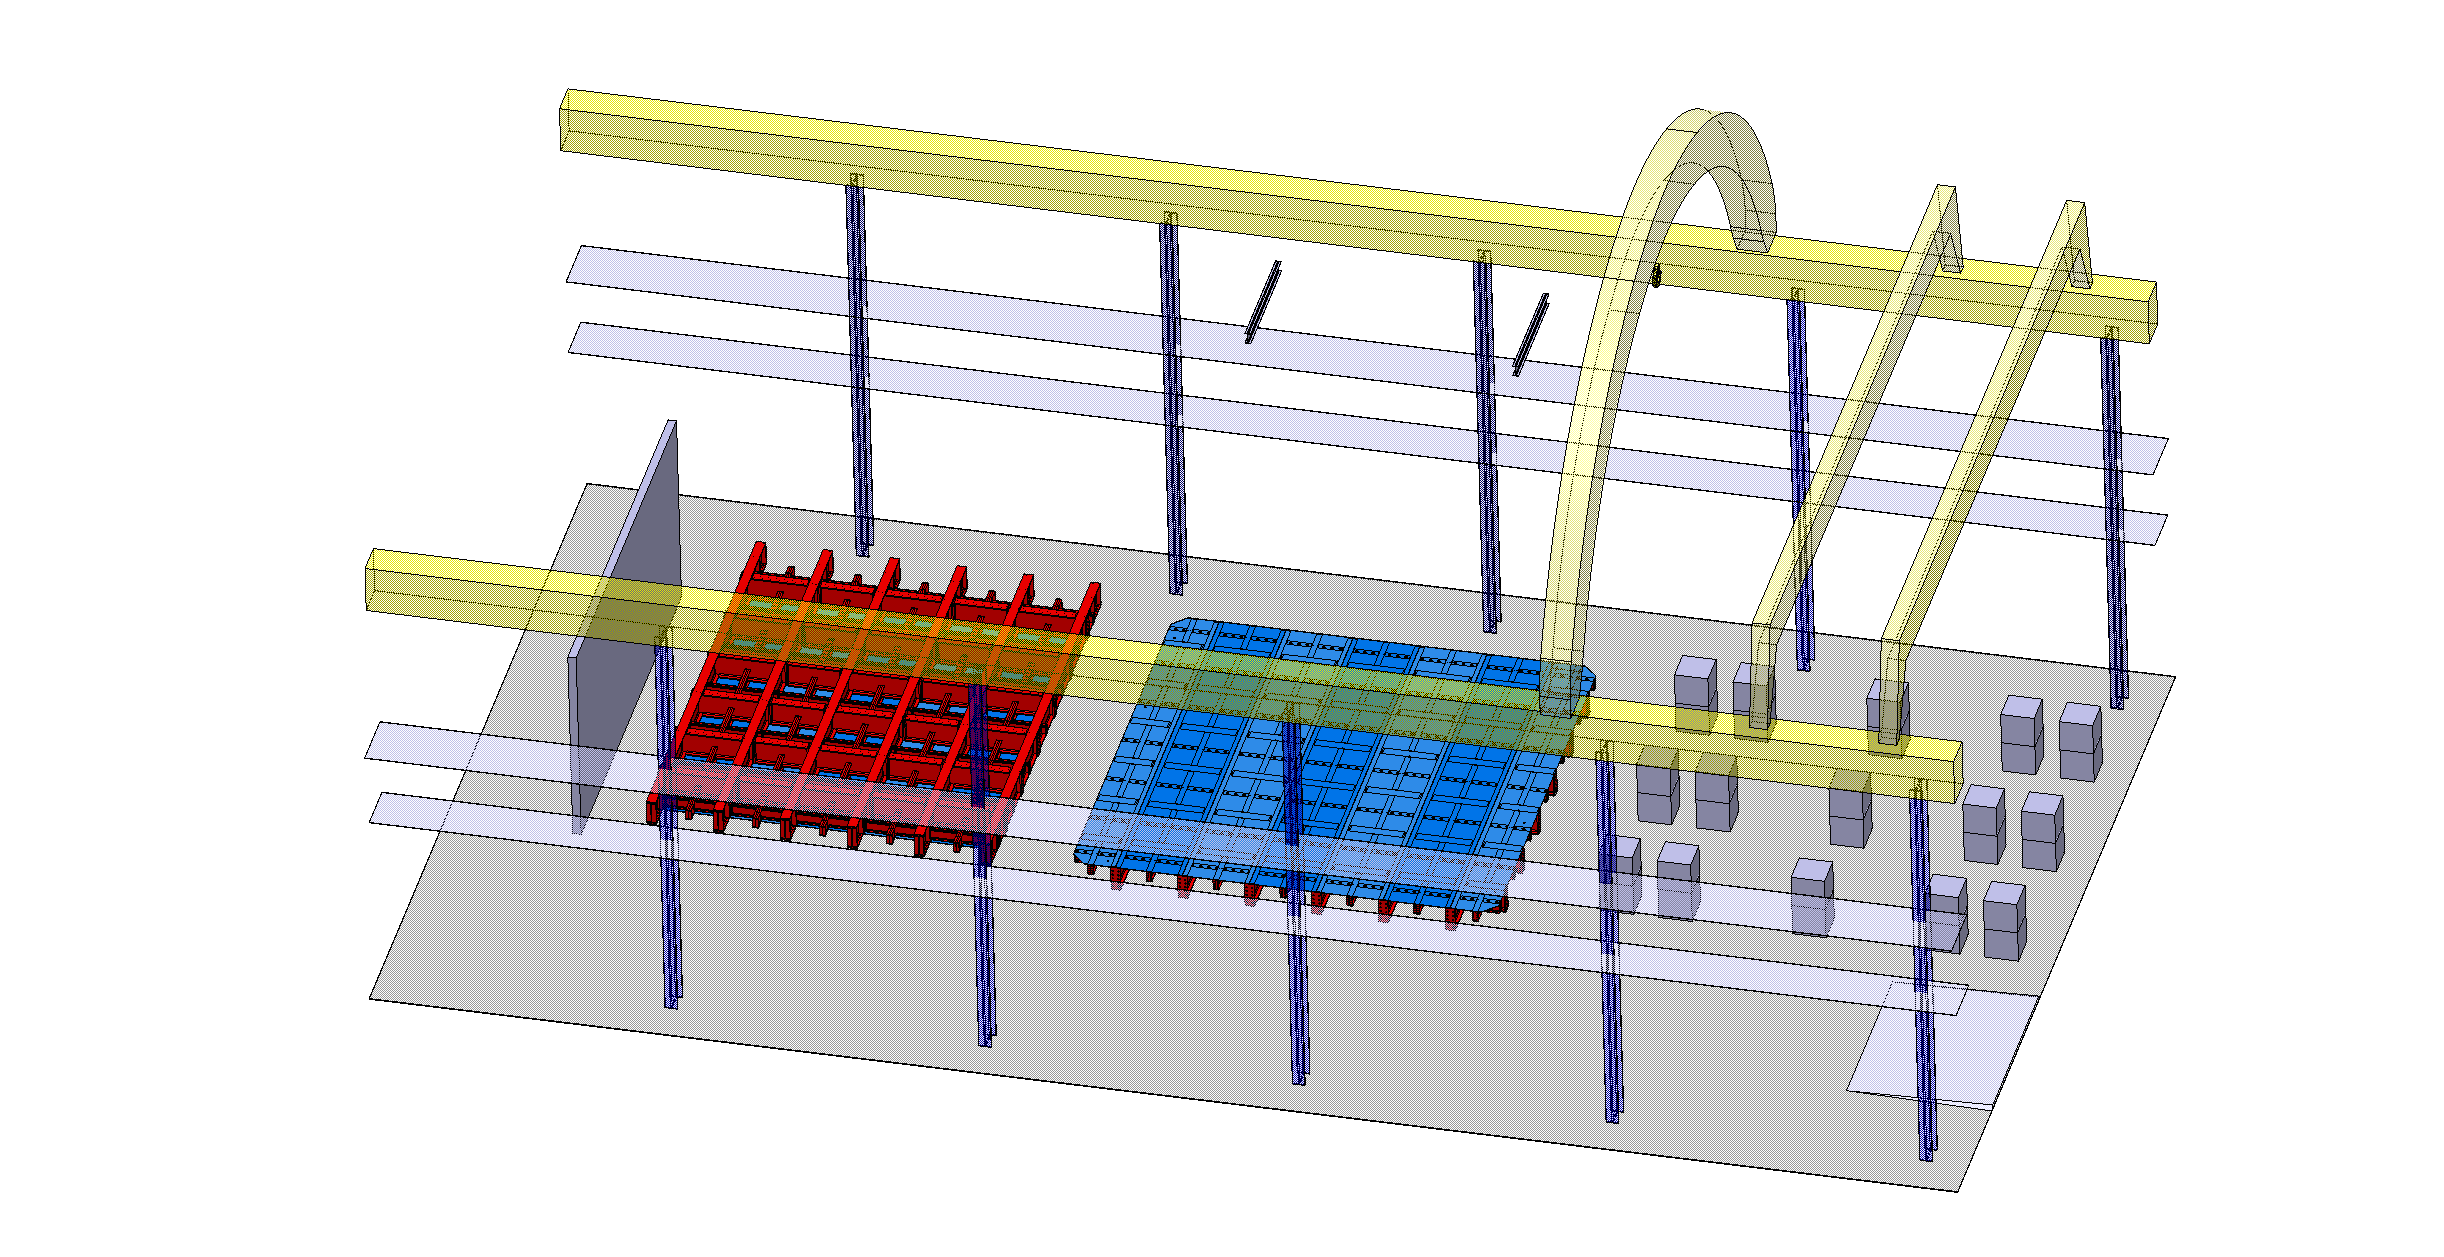
\includegraphics[width=0.32\textwidth]{./Figures/assembly_sequence_11_07/10.png}}
\subfigure[]{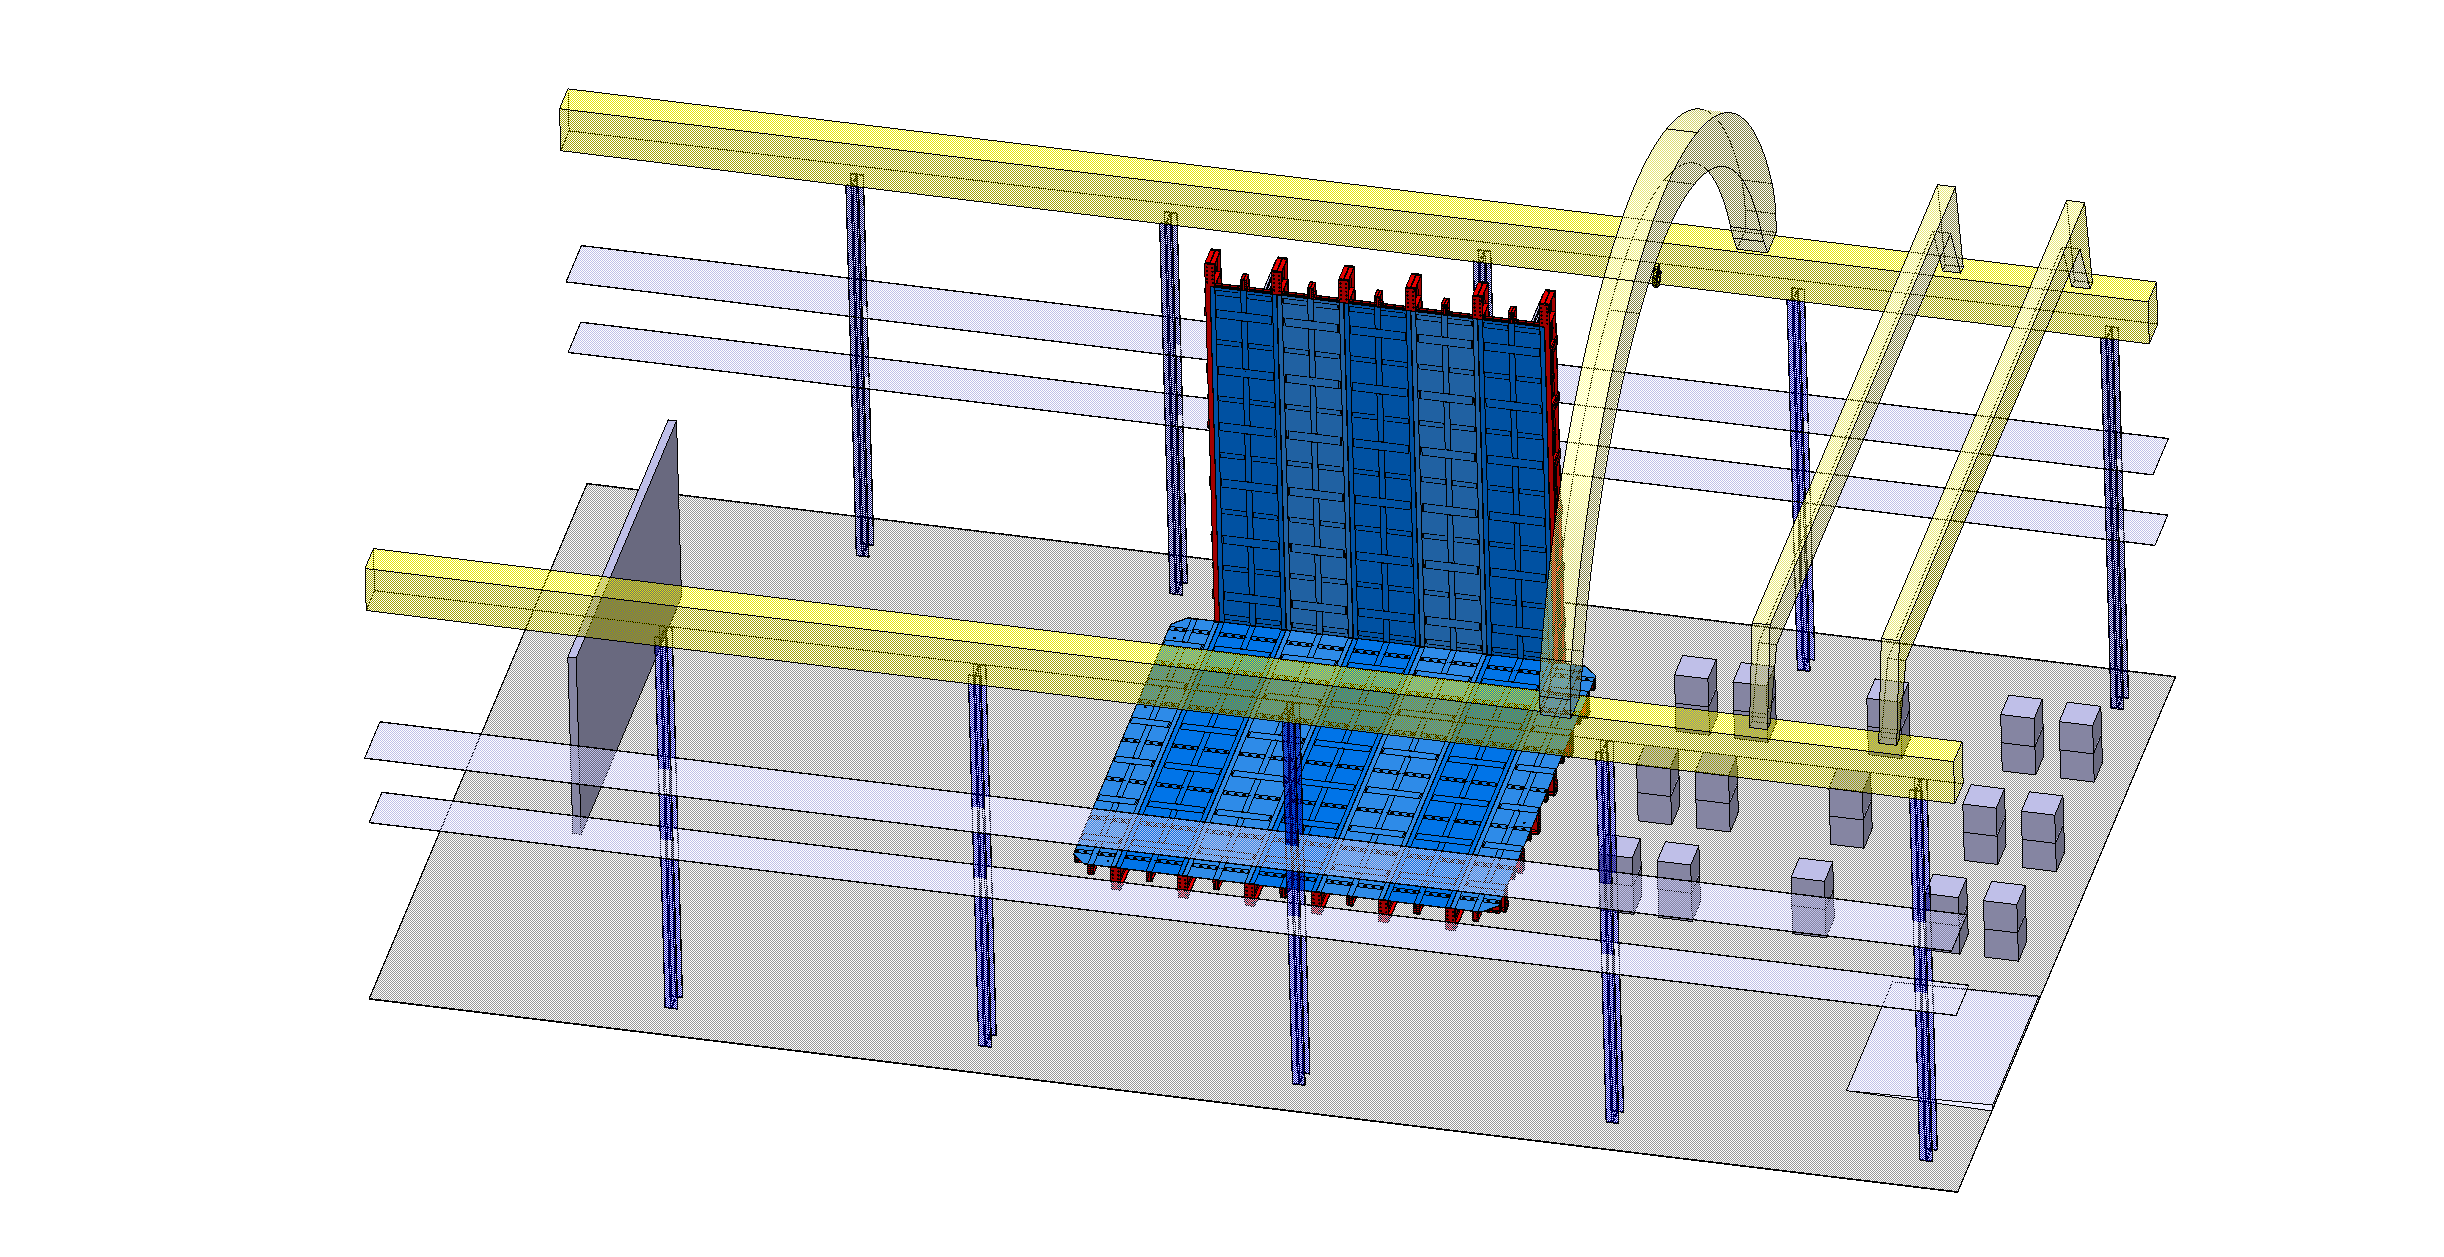
\includegraphics[width=0.32\textwidth]{./Figures/assembly_sequence_11_07/11.png}}
\subfigure[]{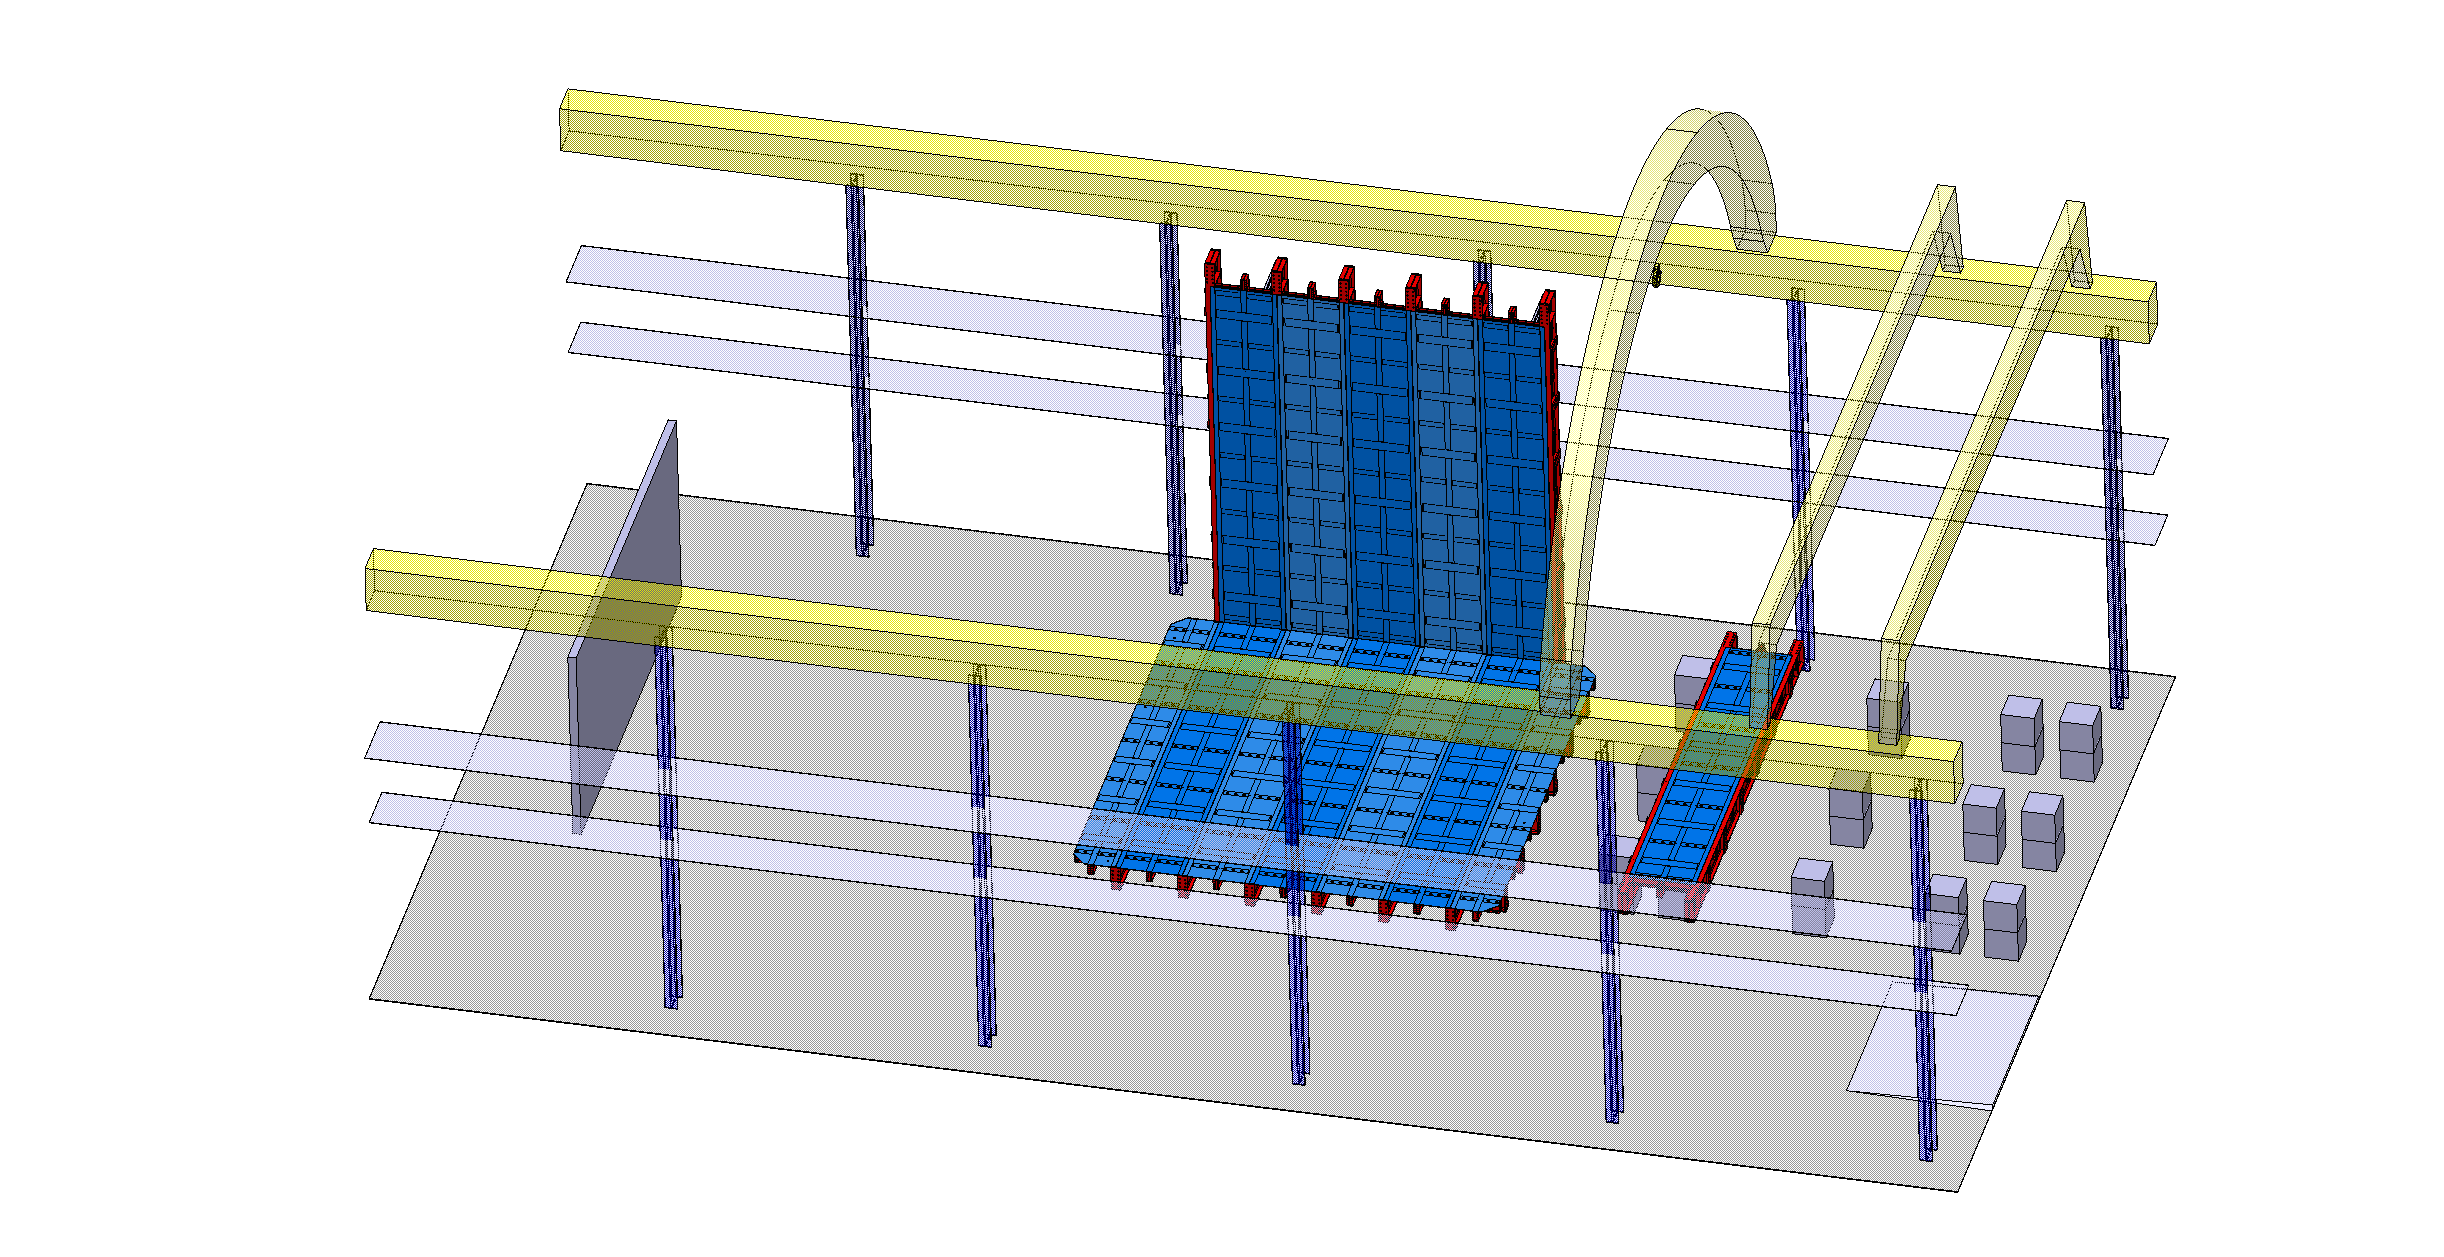
\includegraphics[width=0.32\textwidth]{./Figures/assembly_sequence_11_07/12.png}}
\subfigure[]{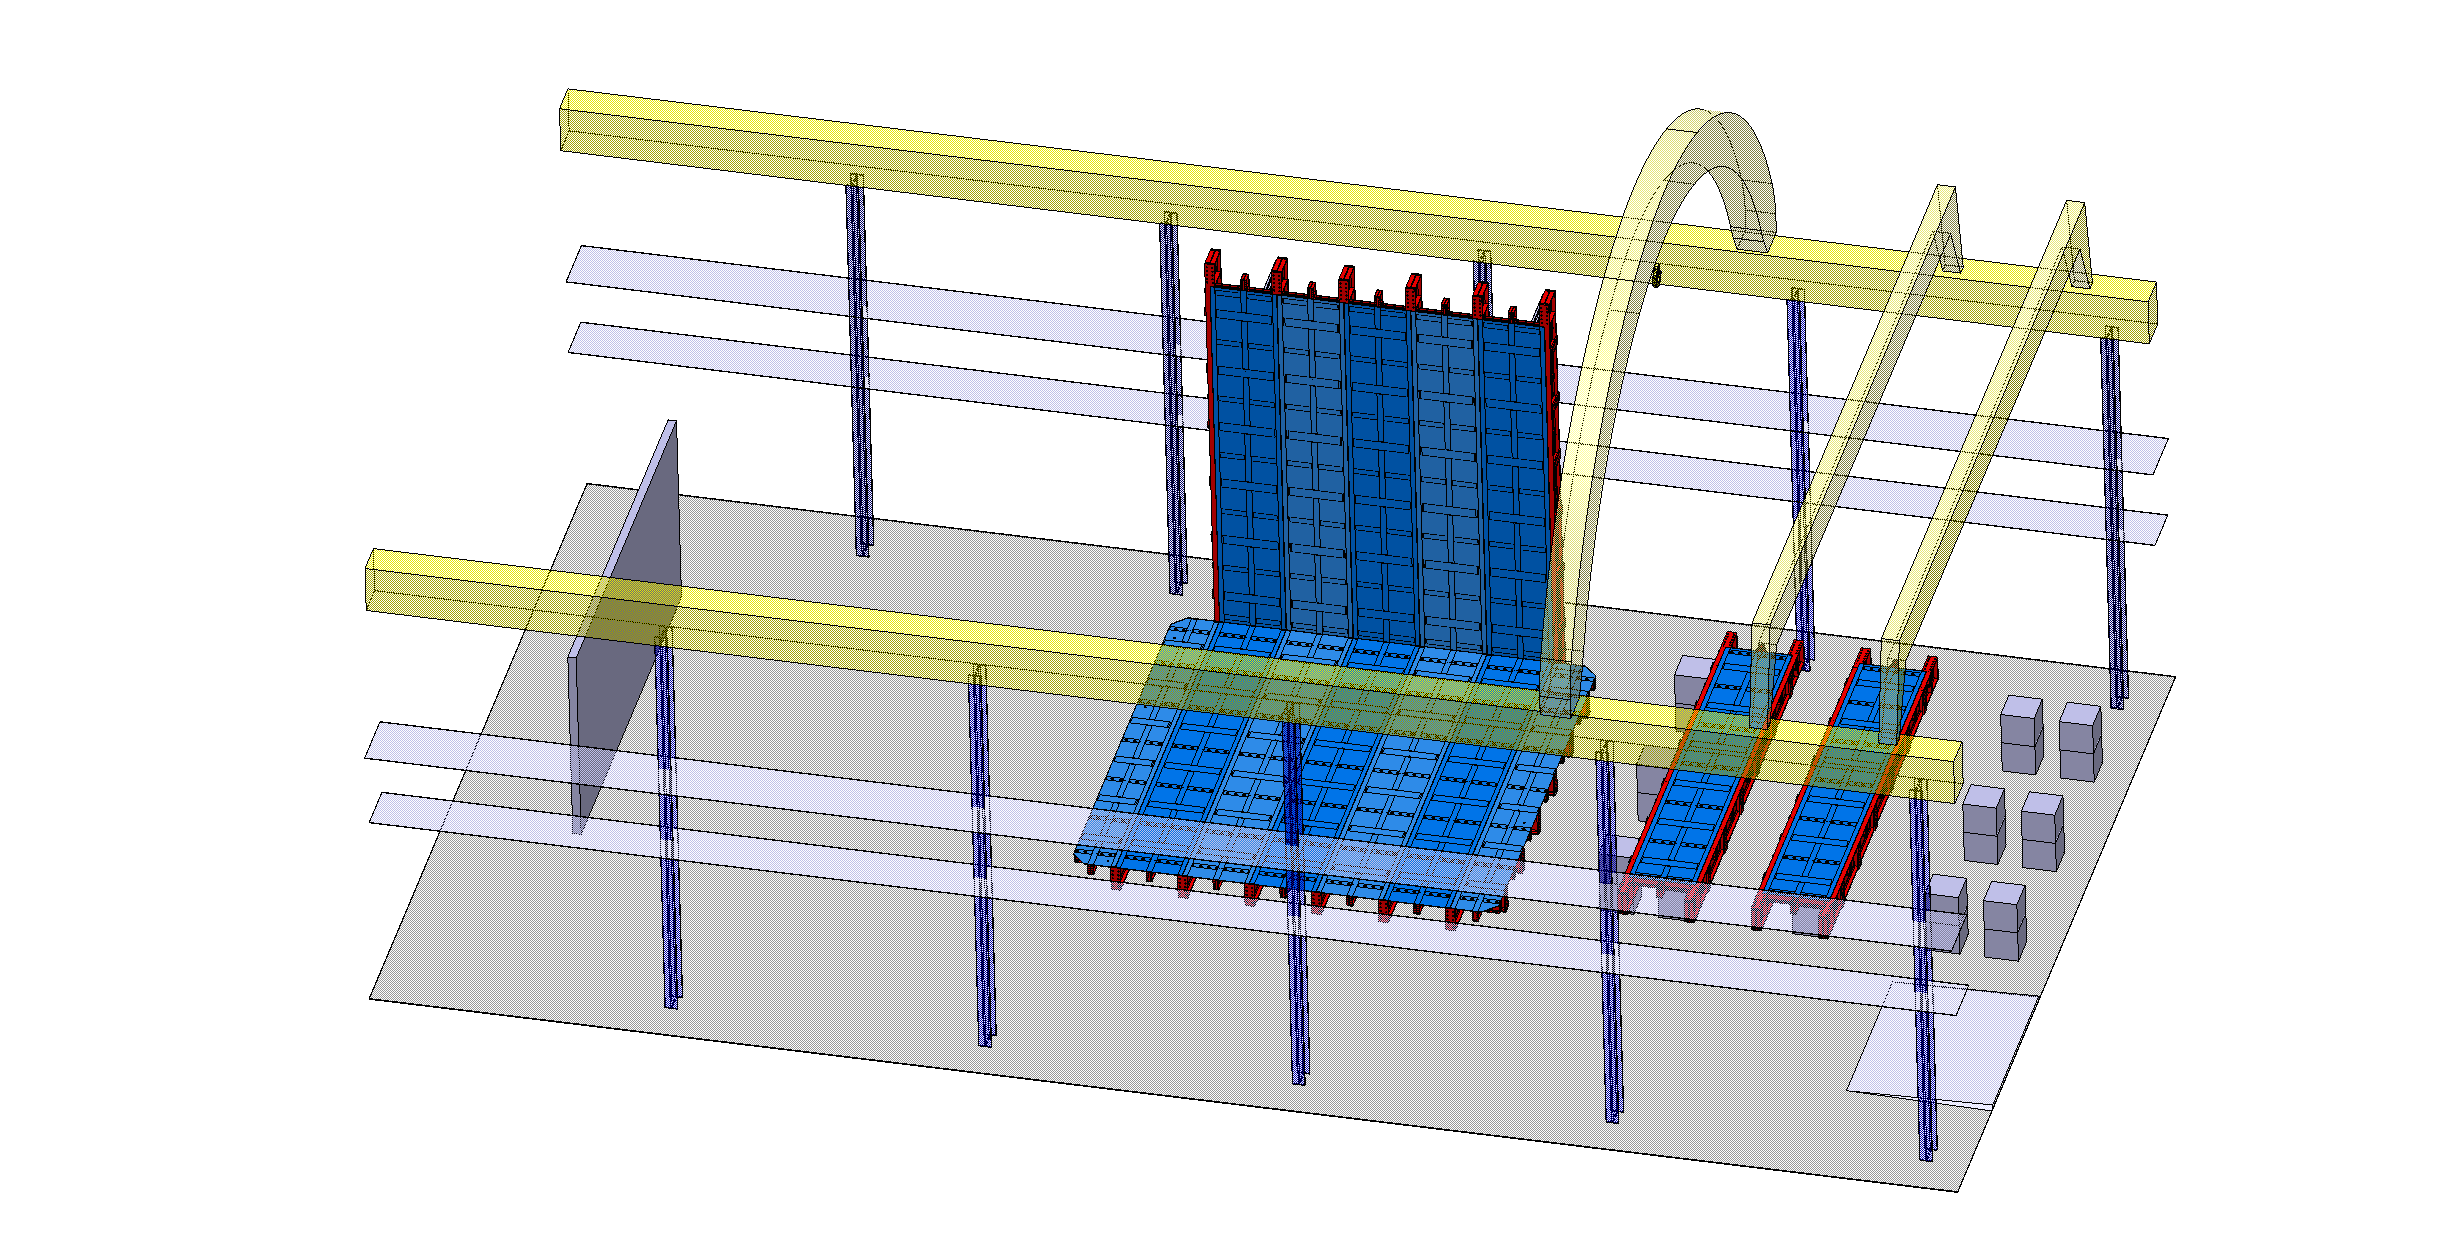
\includegraphics[width=0.32\textwidth]{./Figures/assembly_sequence_11_07/13.png}}
\subfigure[]{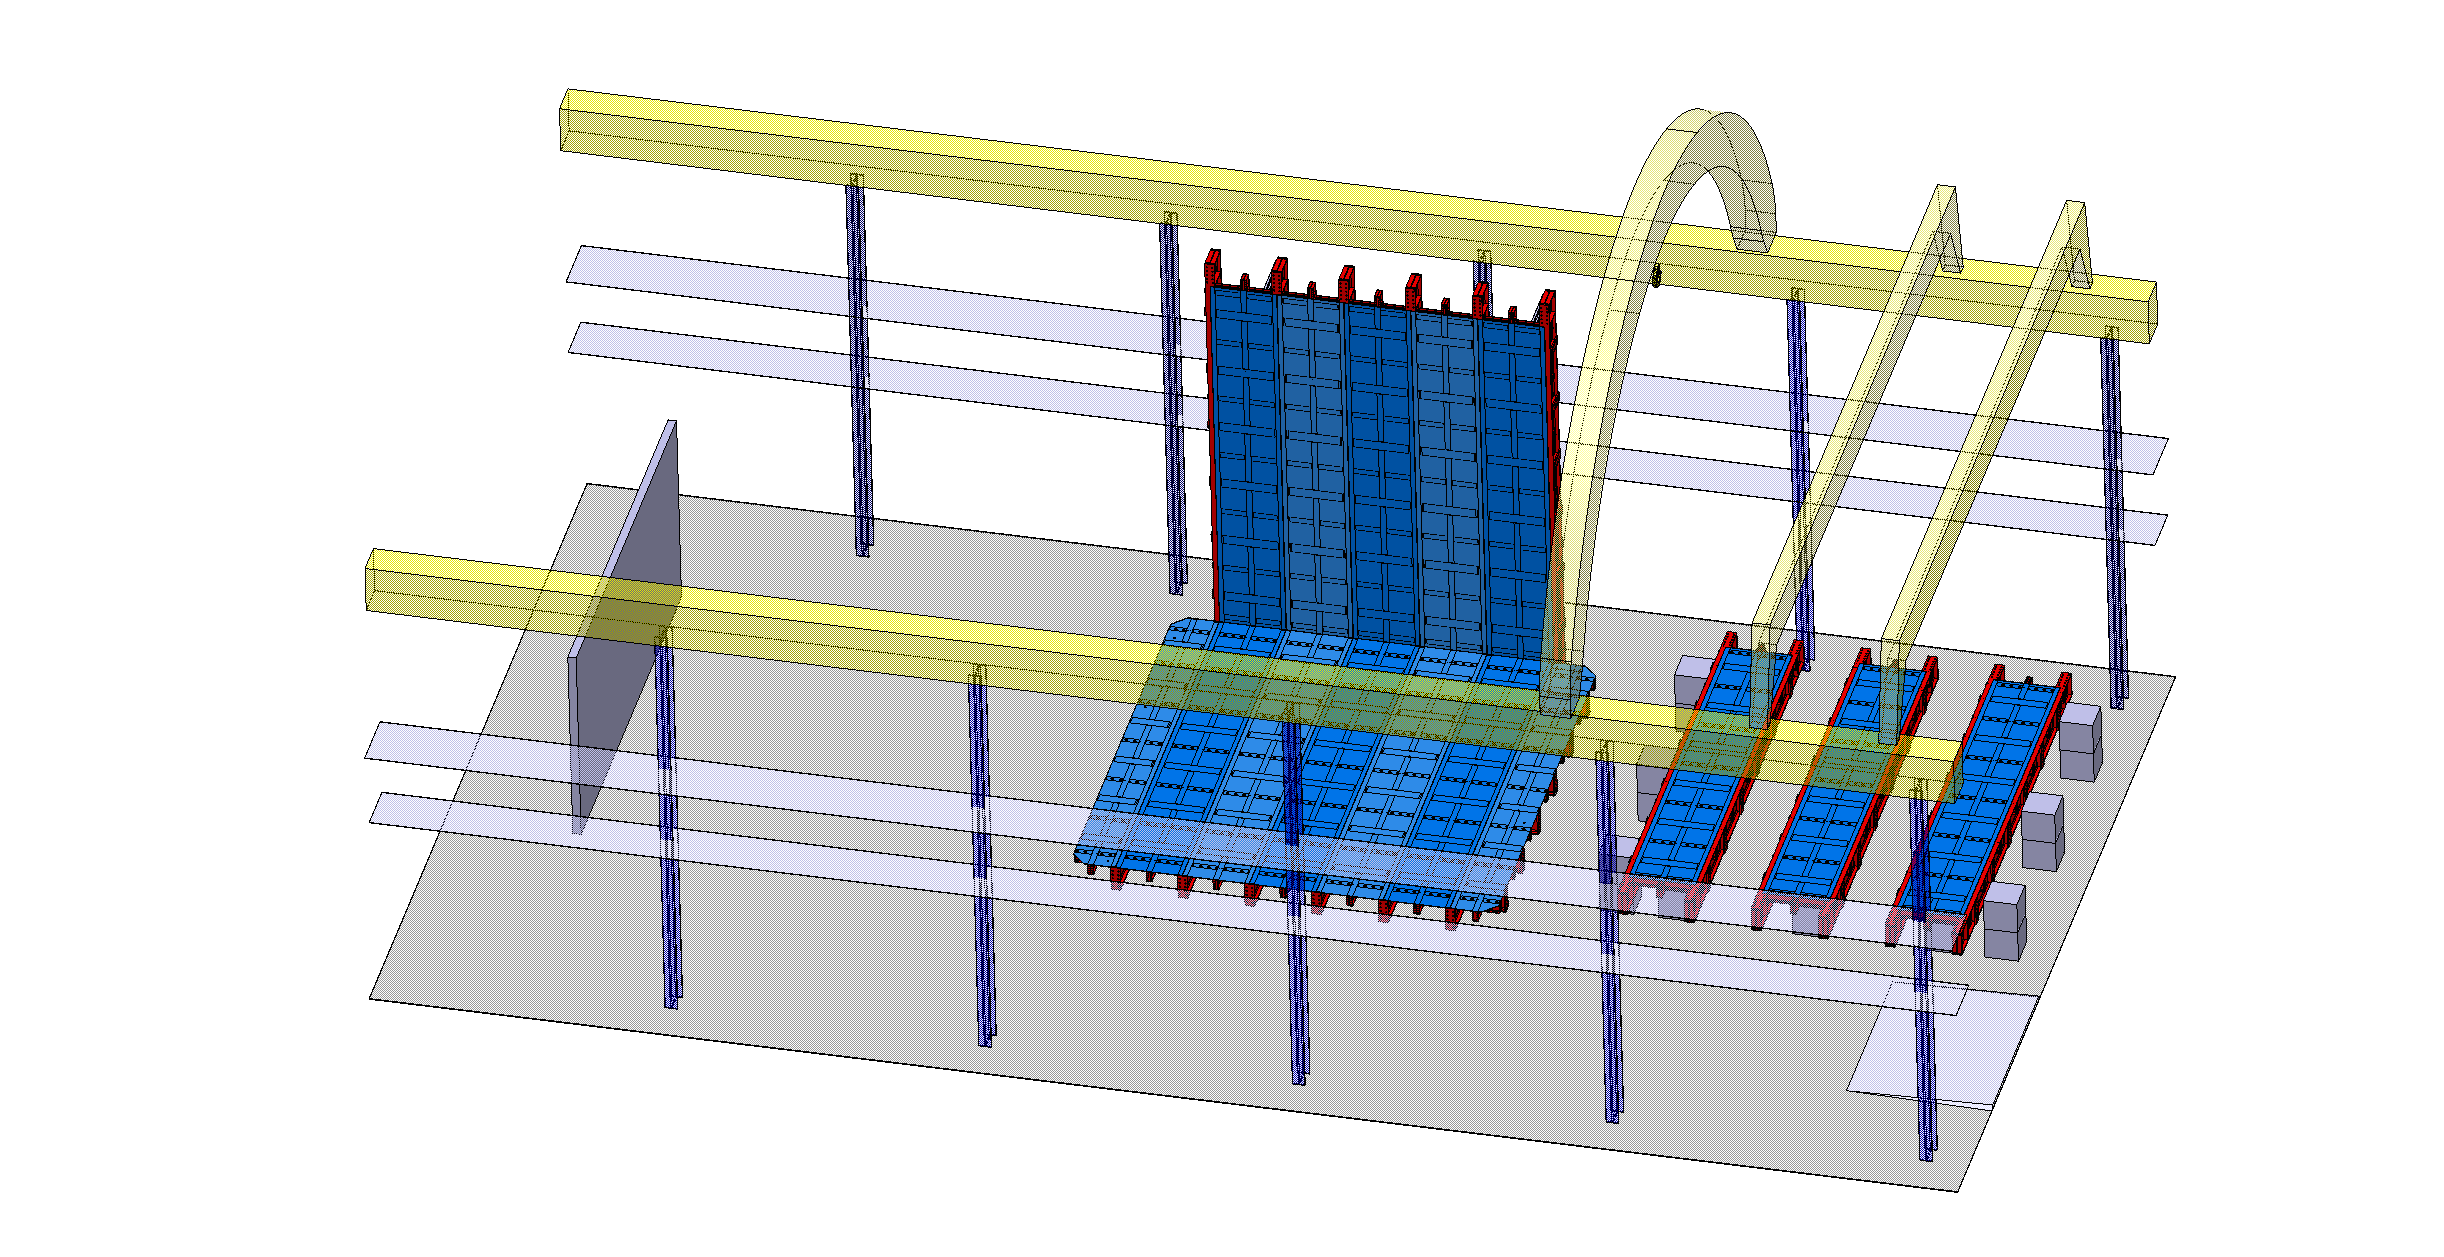
\includegraphics[width=0.32\textwidth]{./Figures/assembly_sequence_11_07/14.png}}
\subfigure[]{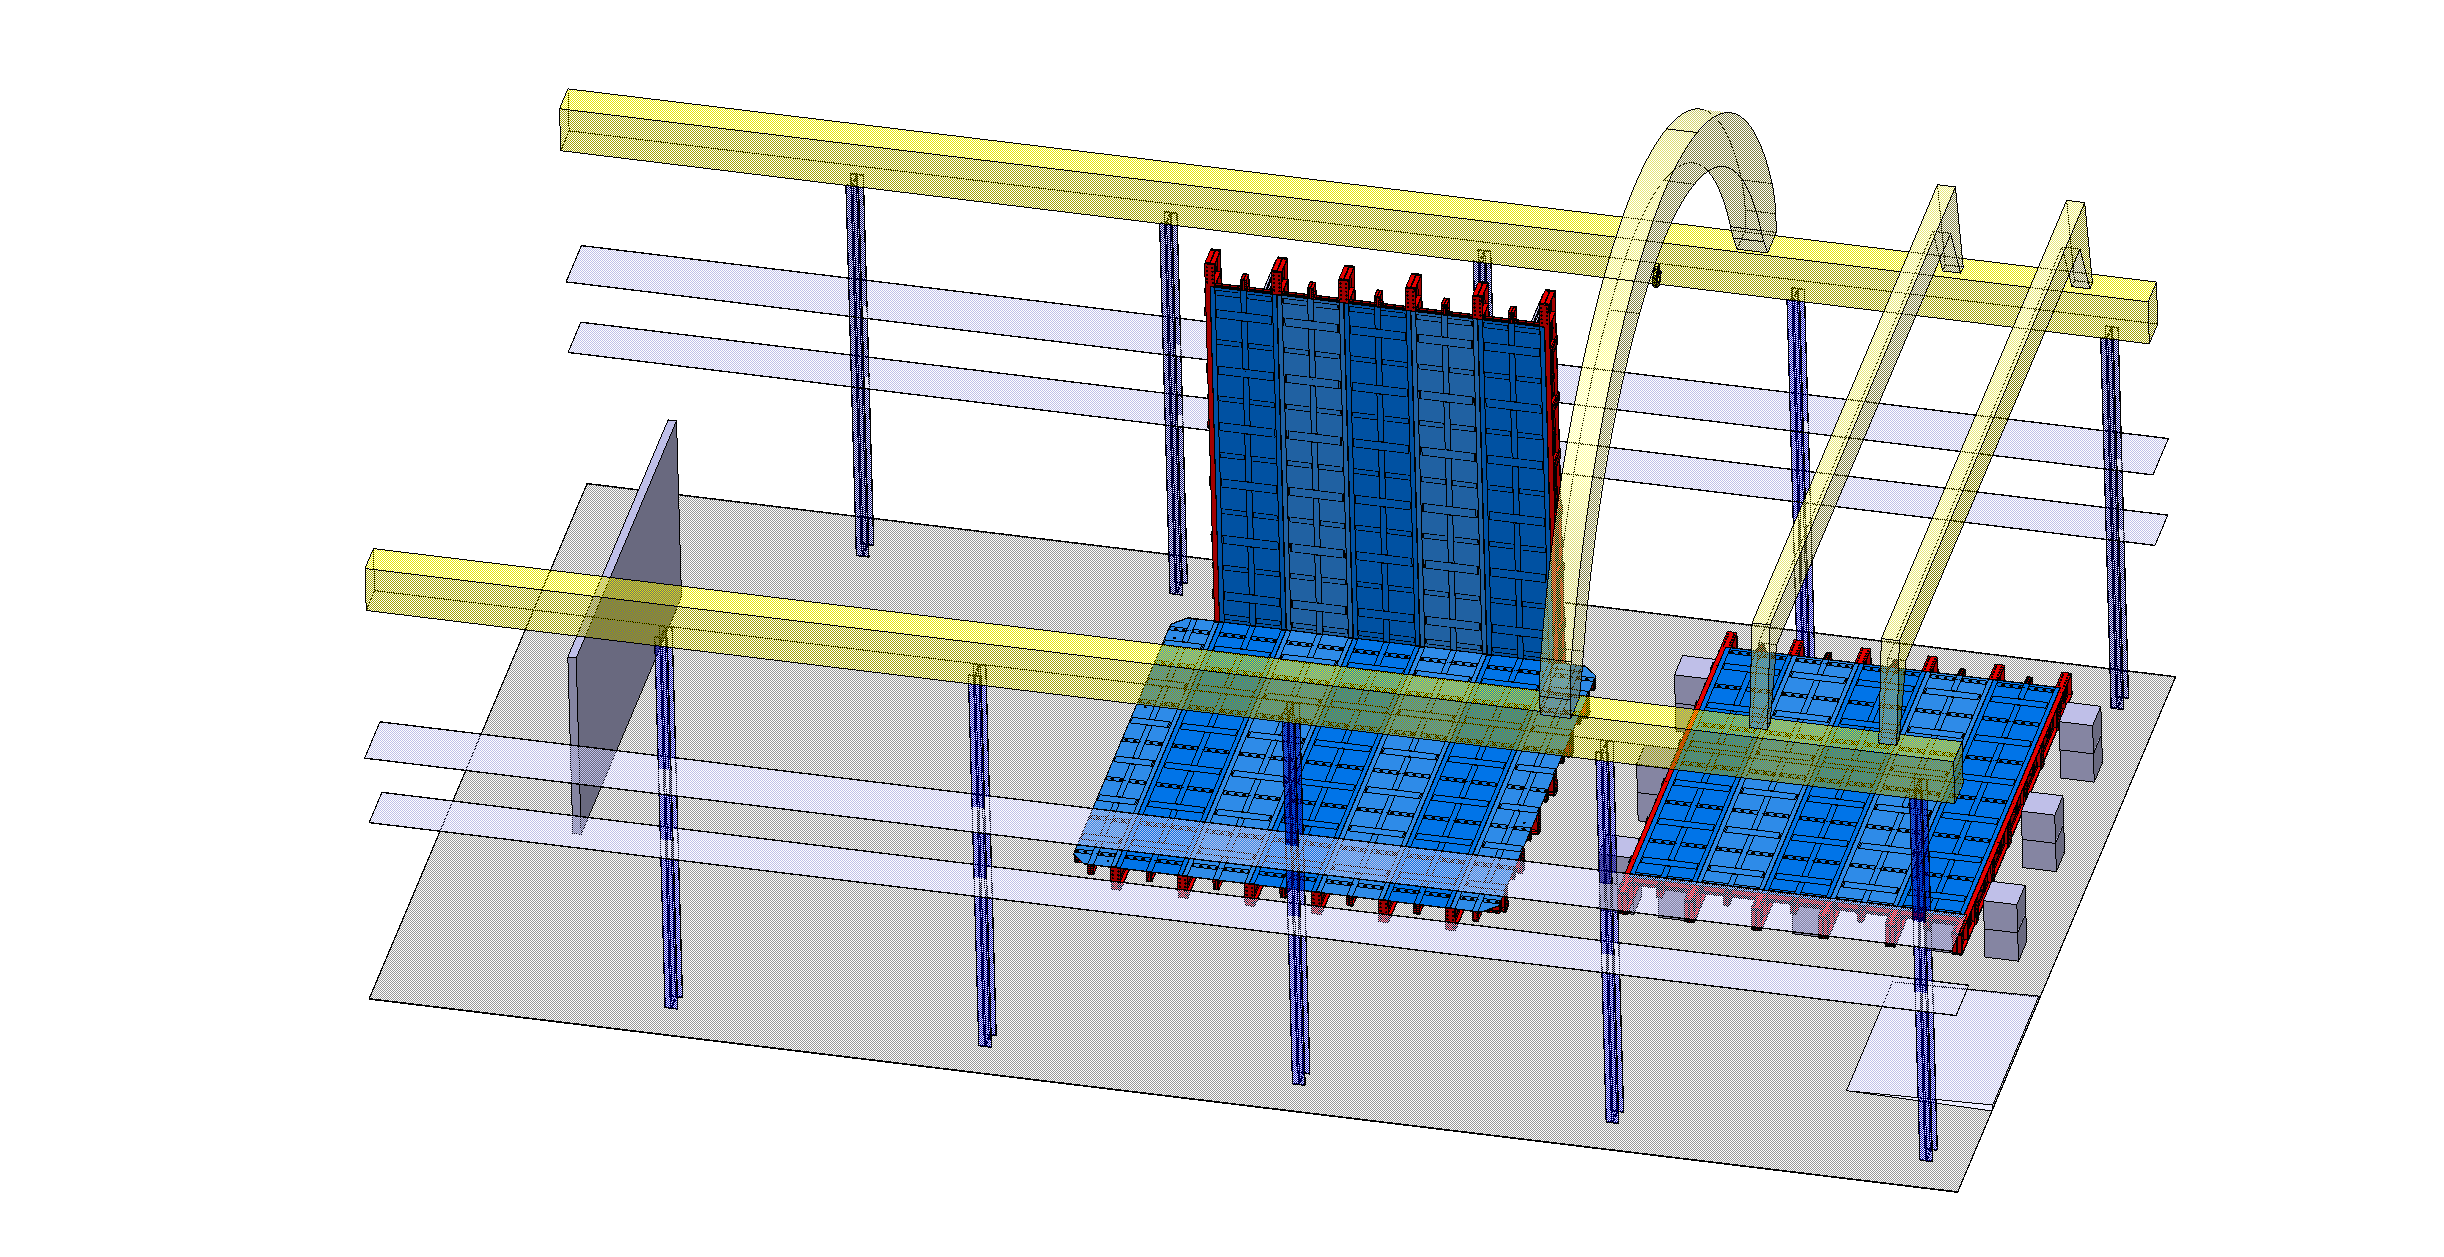
\includegraphics[width=0.32\textwidth]{./Figures/assembly_sequence_11_07/15.png}}
\subfigure[]{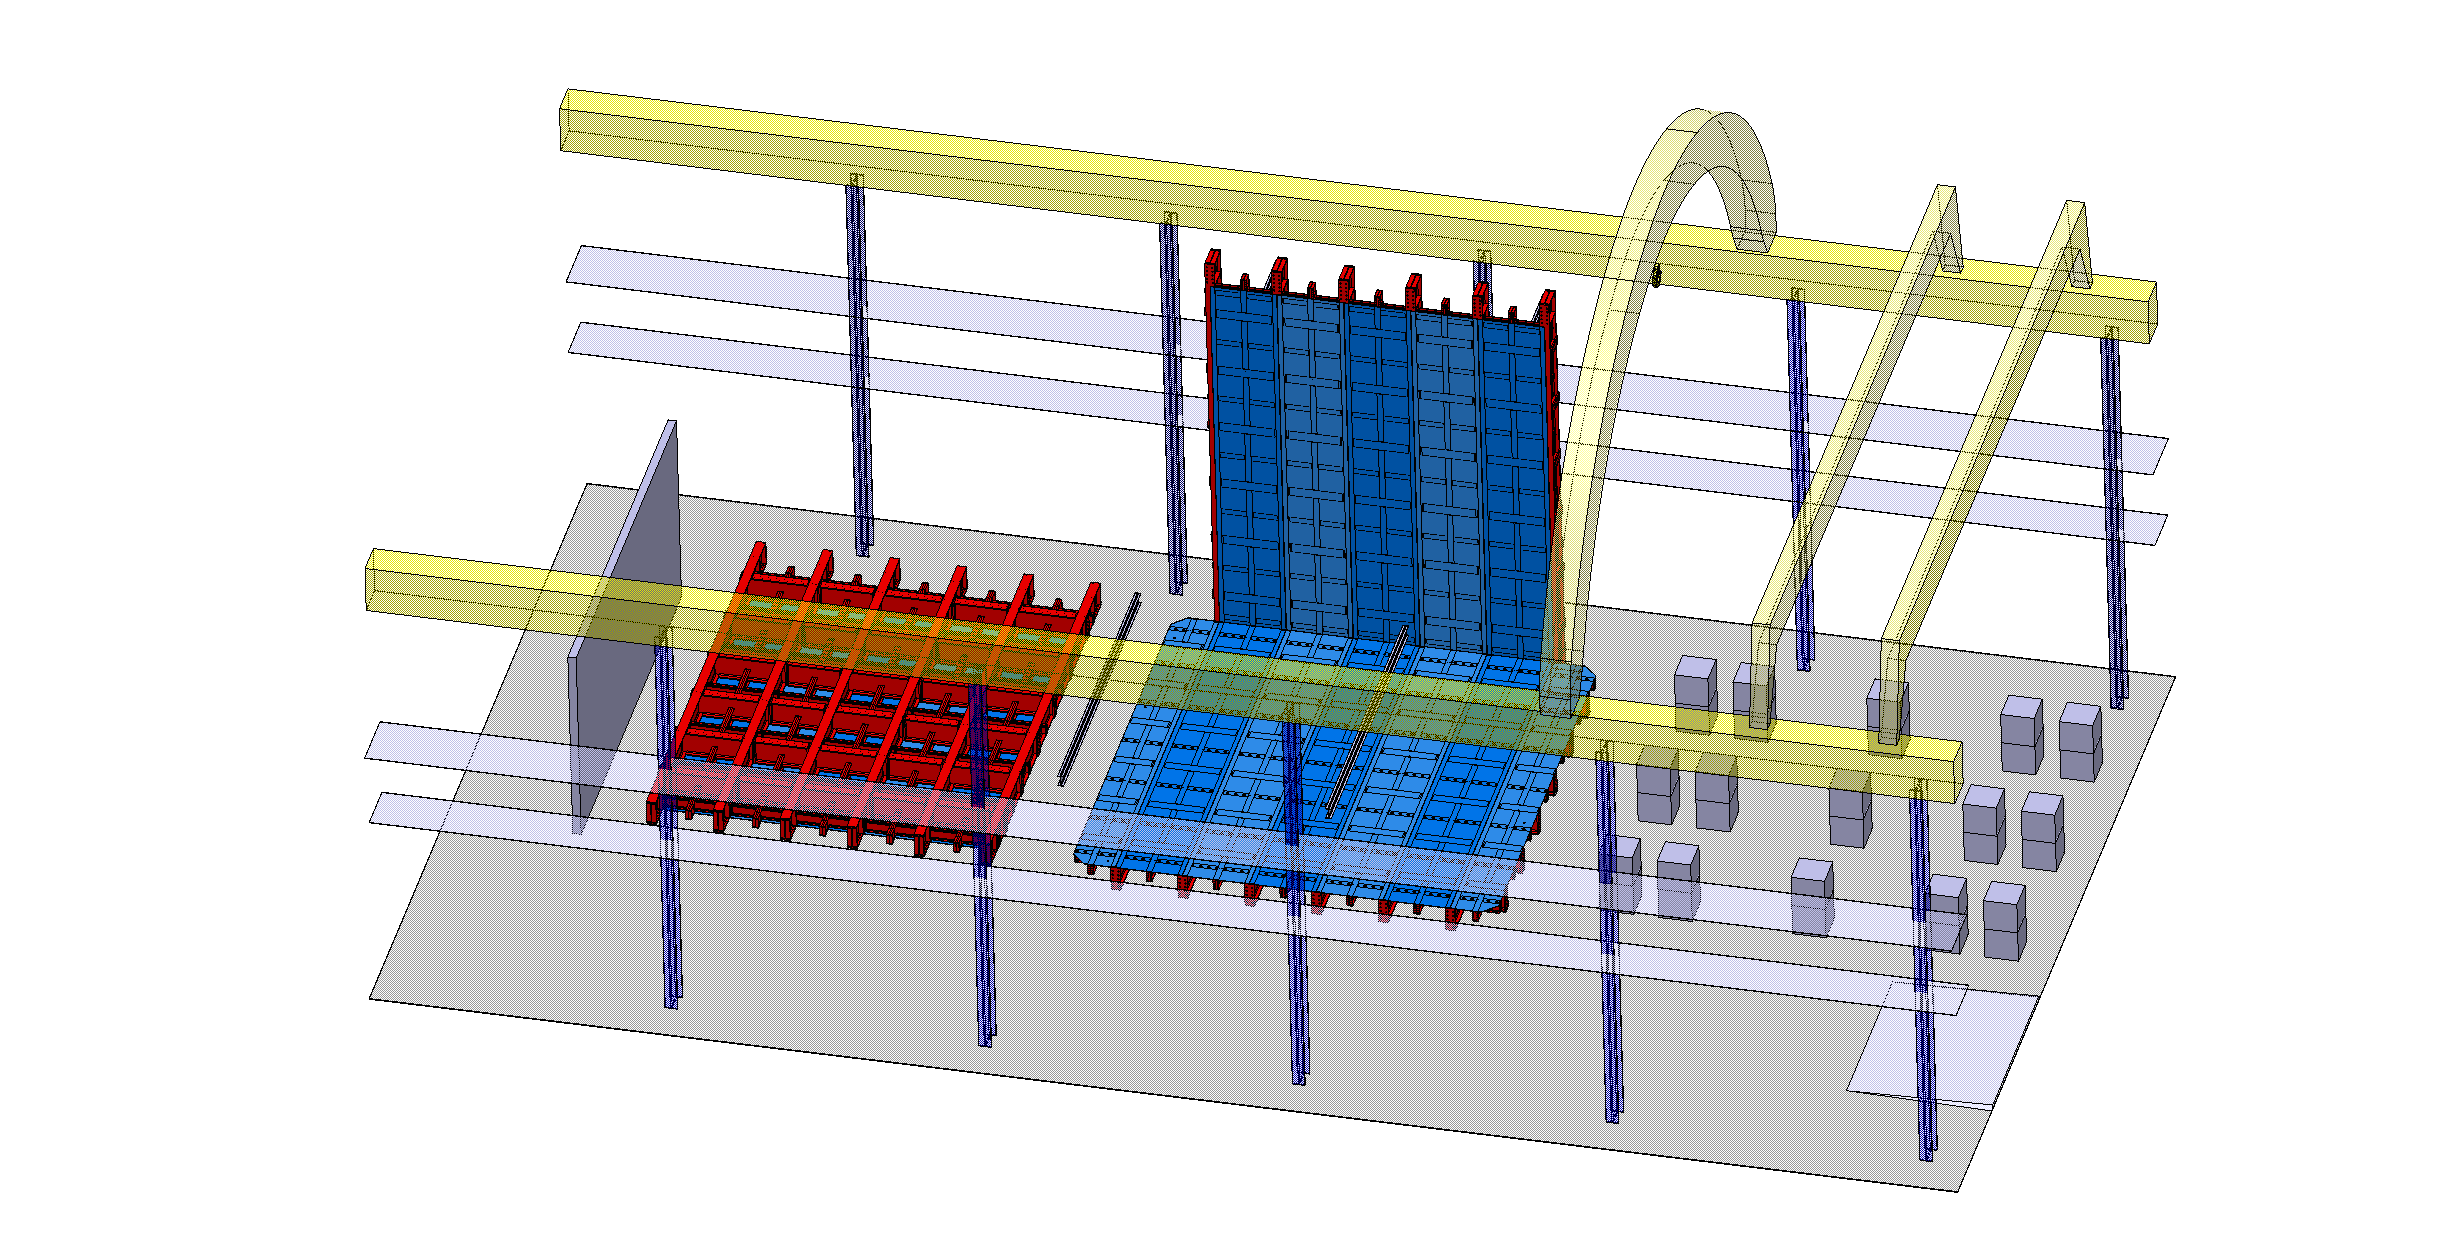
\includegraphics[width=0.32\textwidth]{./Figures/assembly_sequence_11_07/16.png}}
\subfigure[]{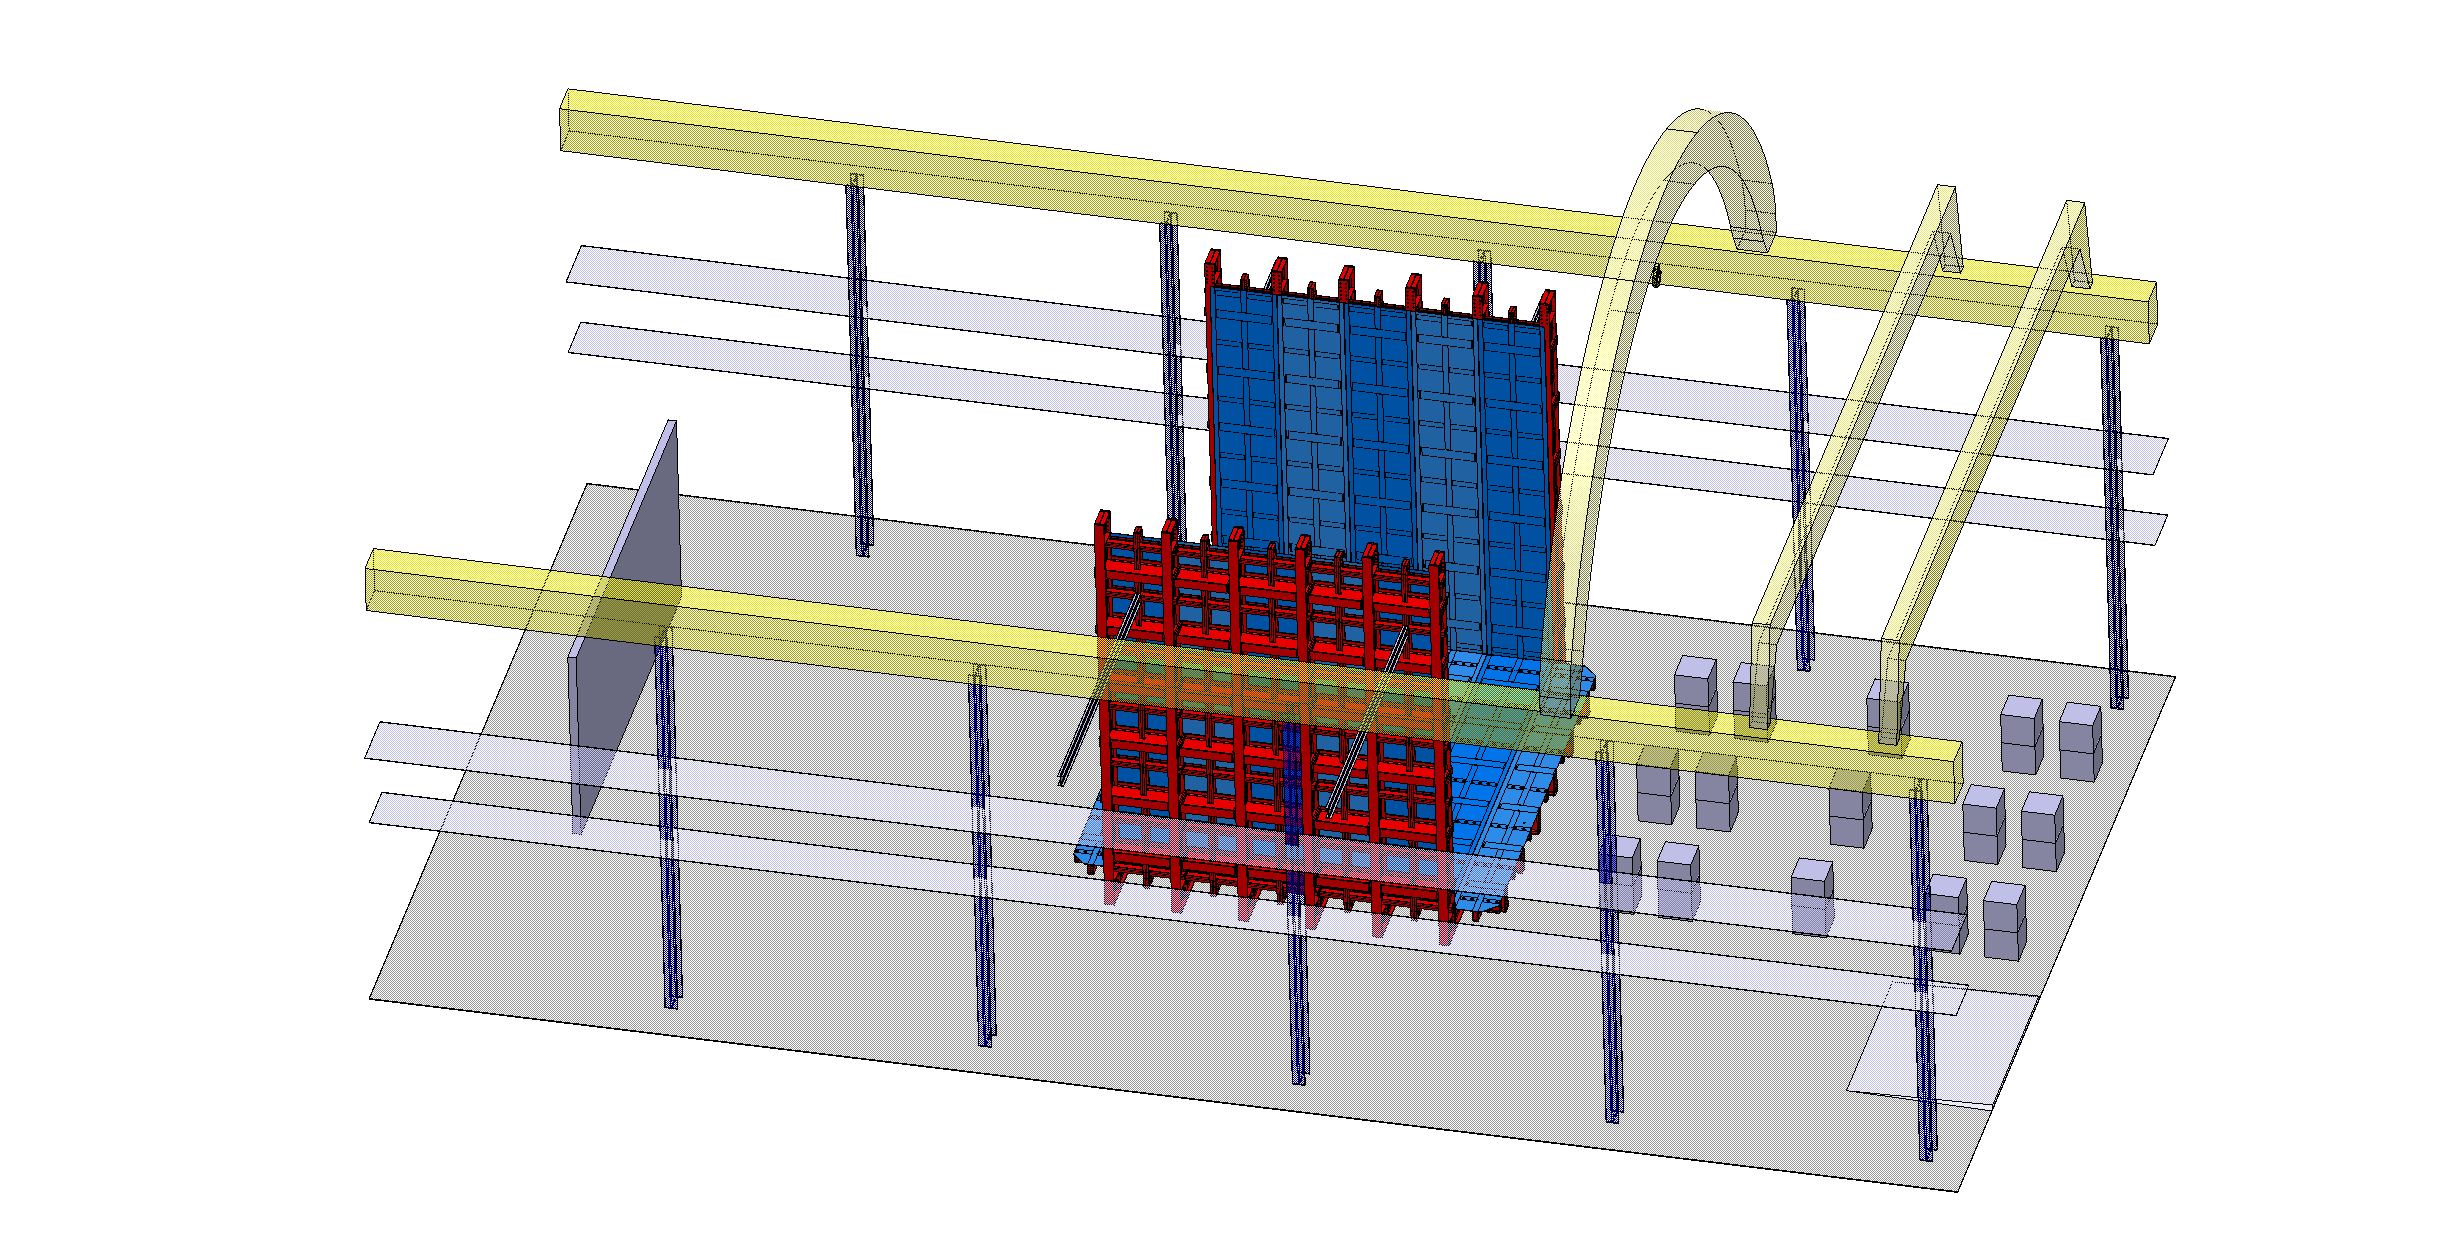
\includegraphics[width=0.32\textwidth]{./Figures/assembly_sequence_11_07/17.png}}
\caption{Details of the installation sequence (I)}
\label{fig:Ds20kInstallSequence1}
\end{figure*}

\begin{figure*}[!t]
\subfigure[]{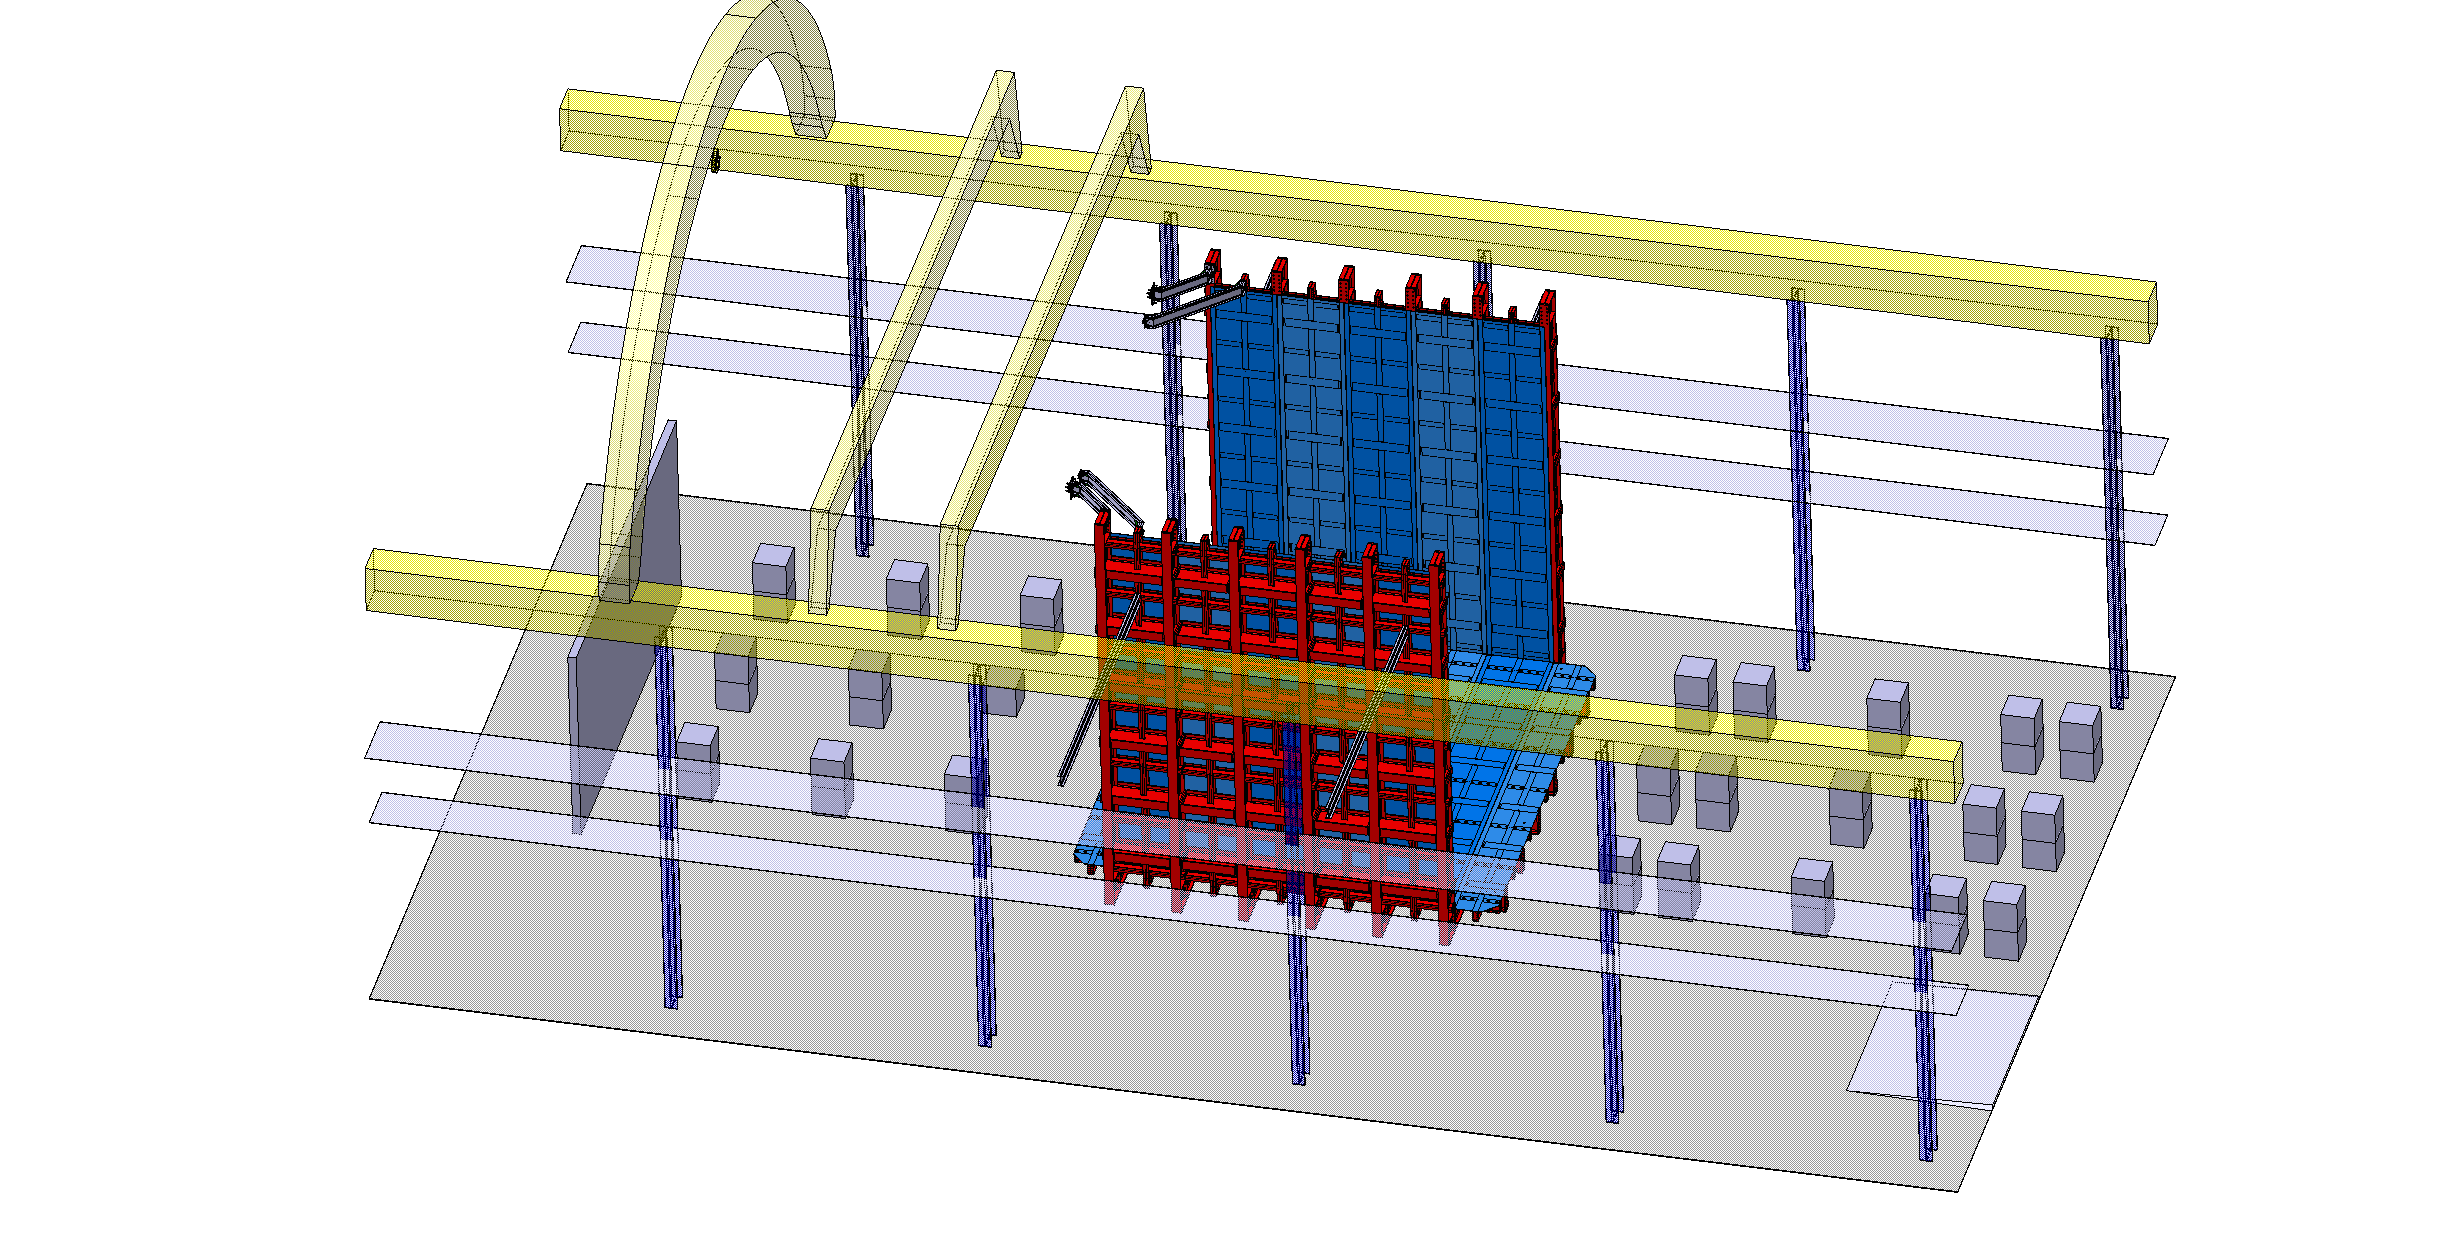
\includegraphics[width=0.32\textwidth]{./Figures/assembly_sequence_11_07/18.png}}
\subfigure[]{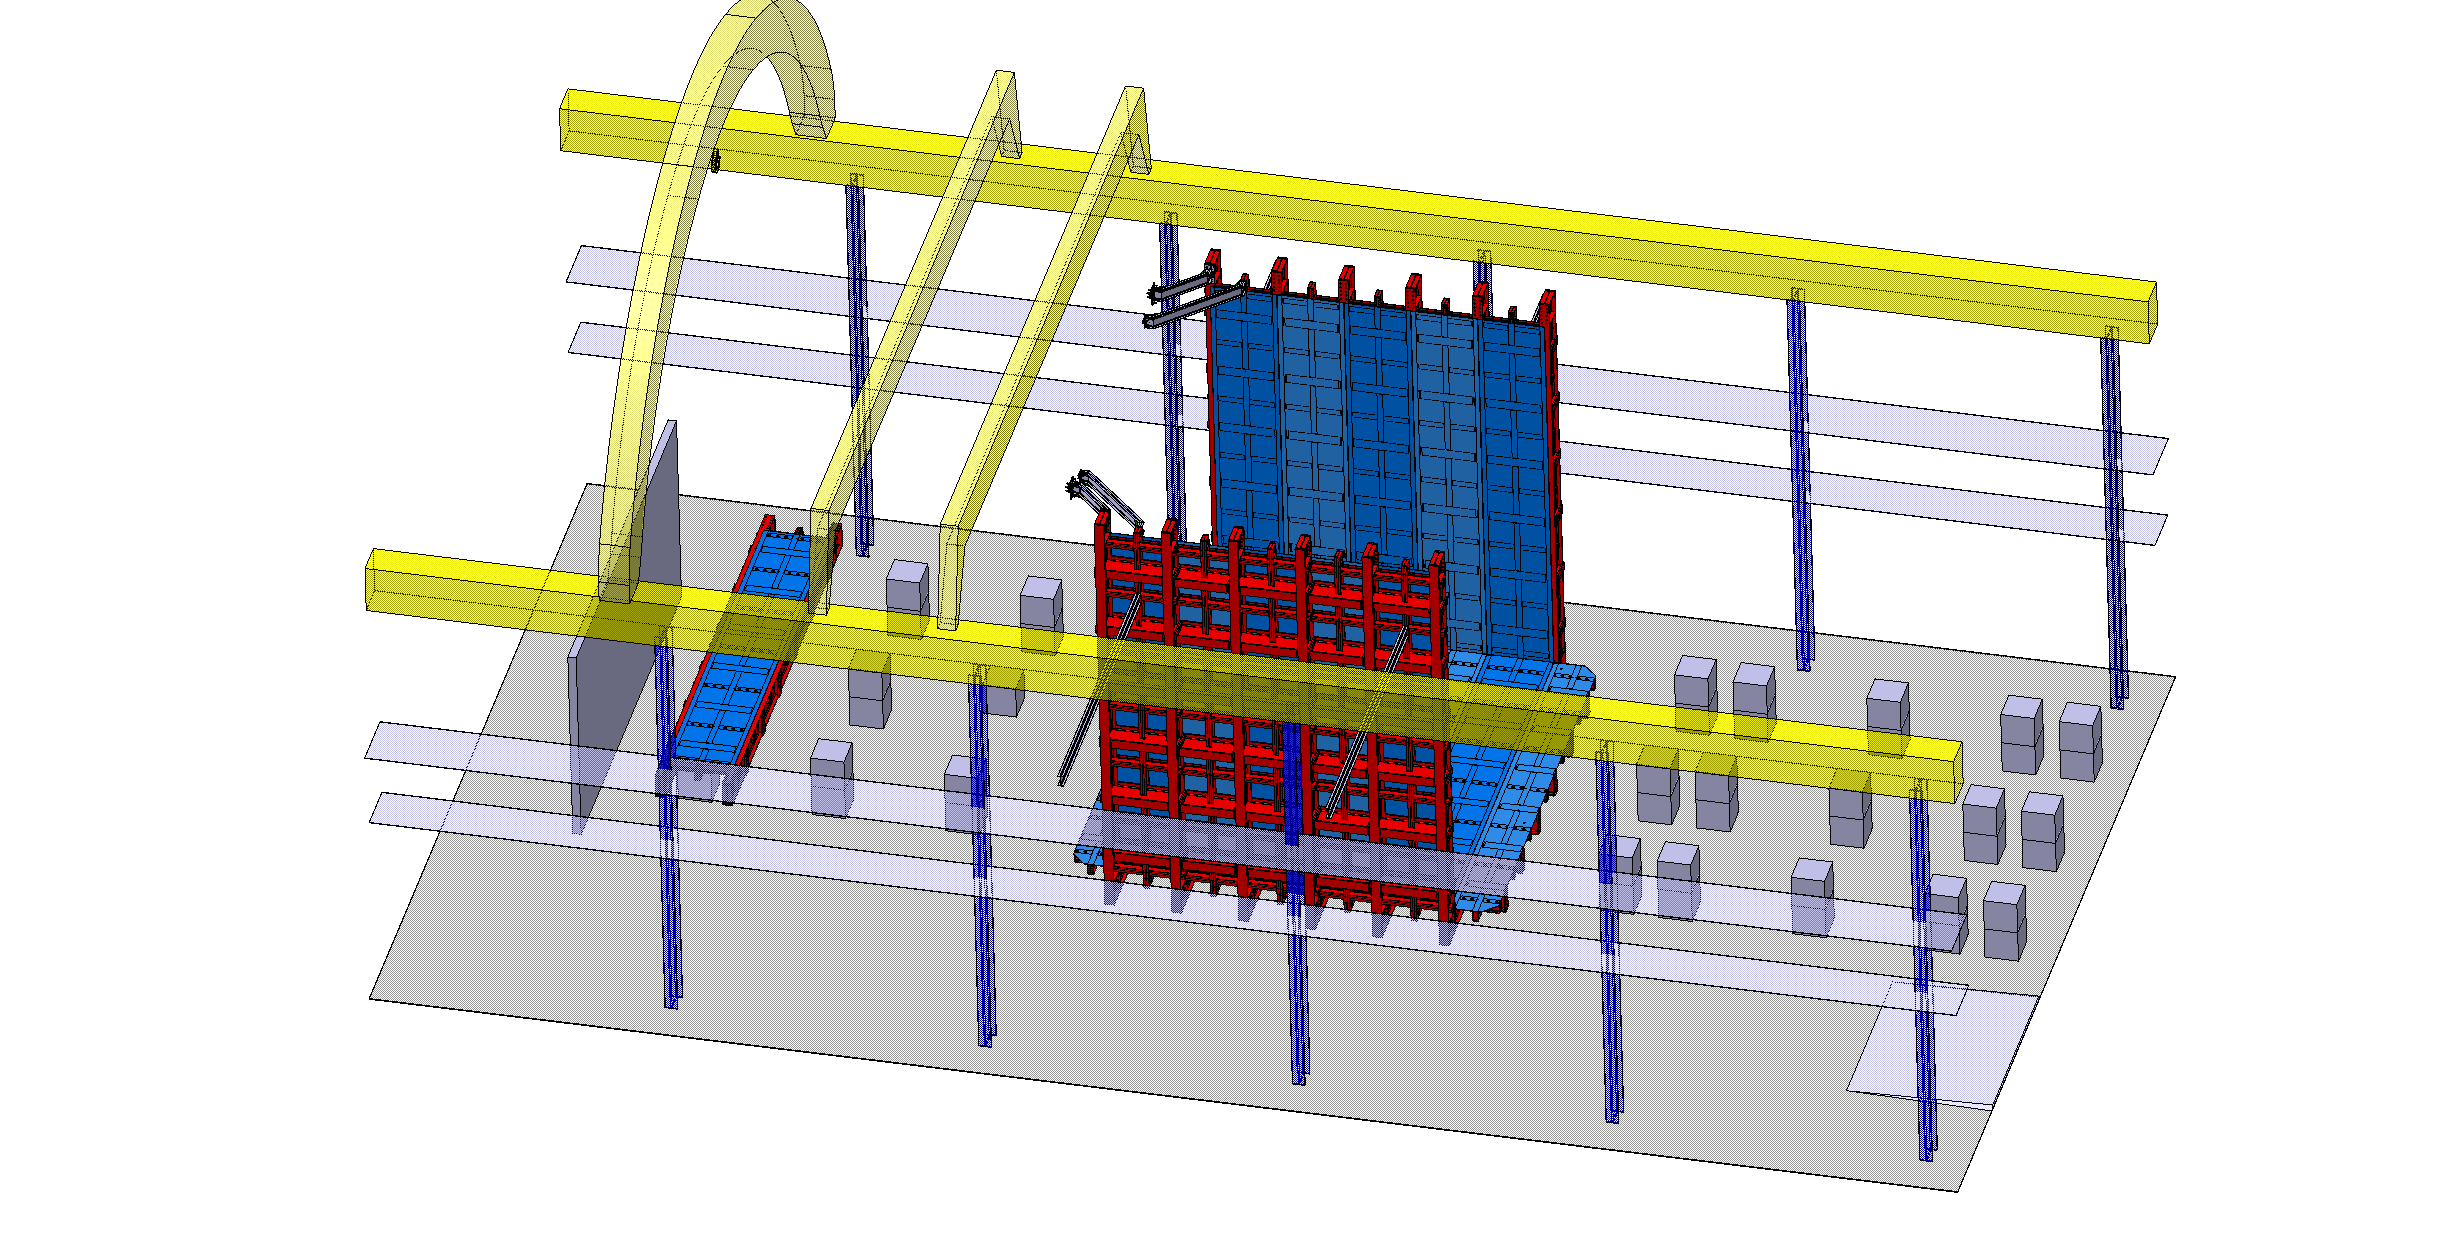
\includegraphics[width=0.32\textwidth]{./Figures/assembly_sequence_11_07/19.png}}
\subfigure[]{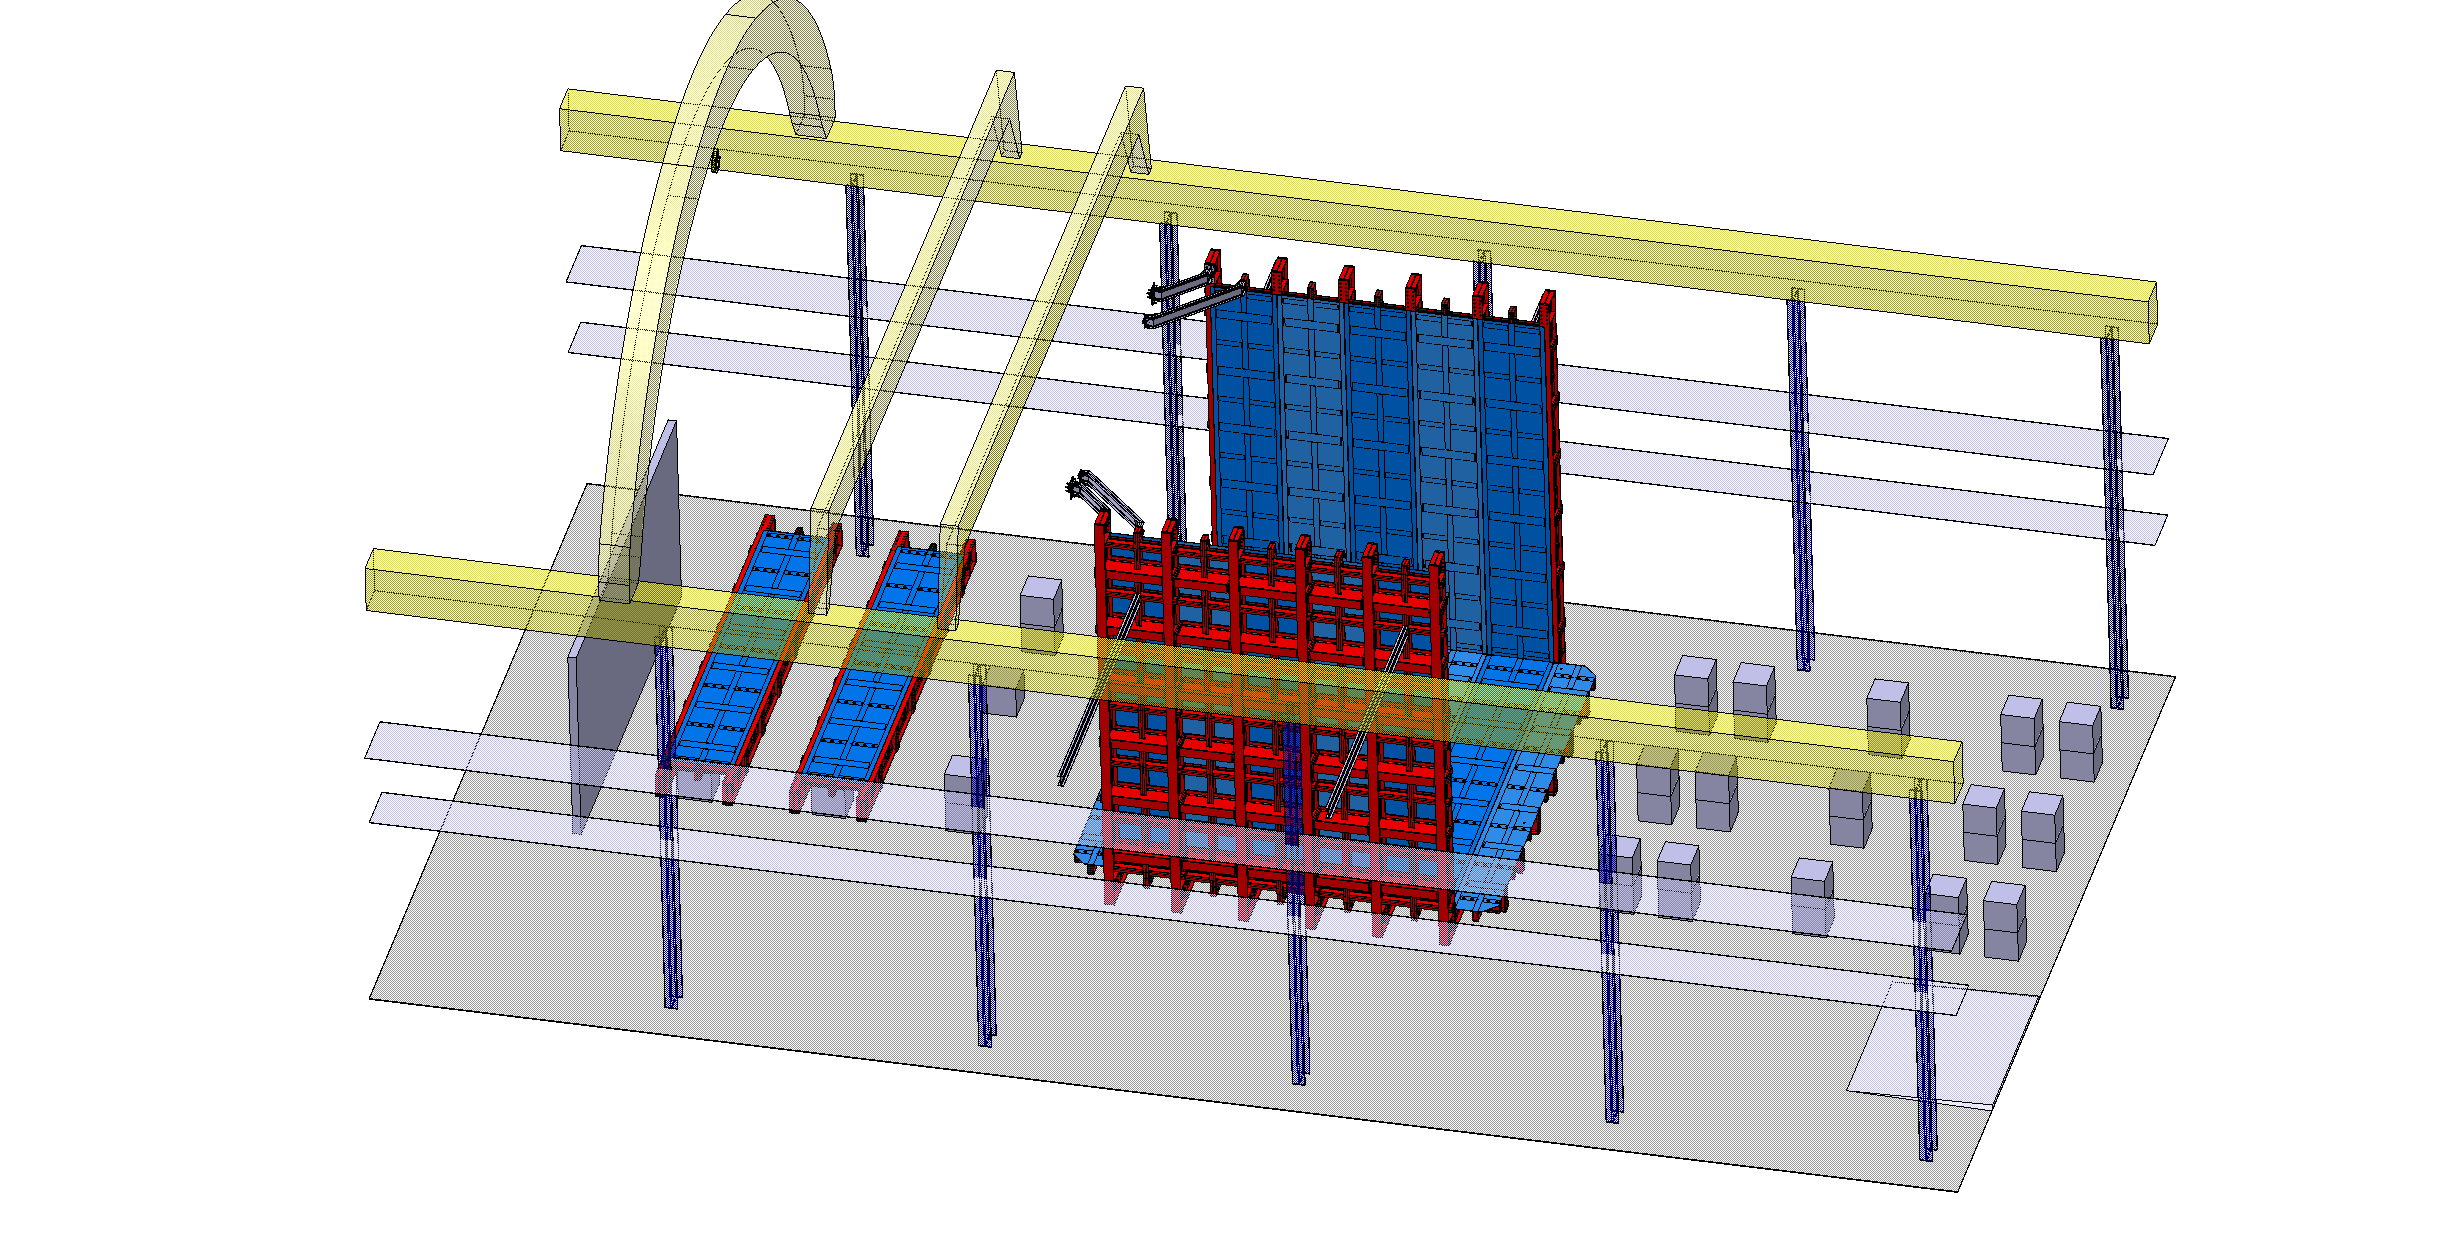
\includegraphics[width=0.32\textwidth]{./Figures/assembly_sequence_11_07/20.png}}
\subfigure[]{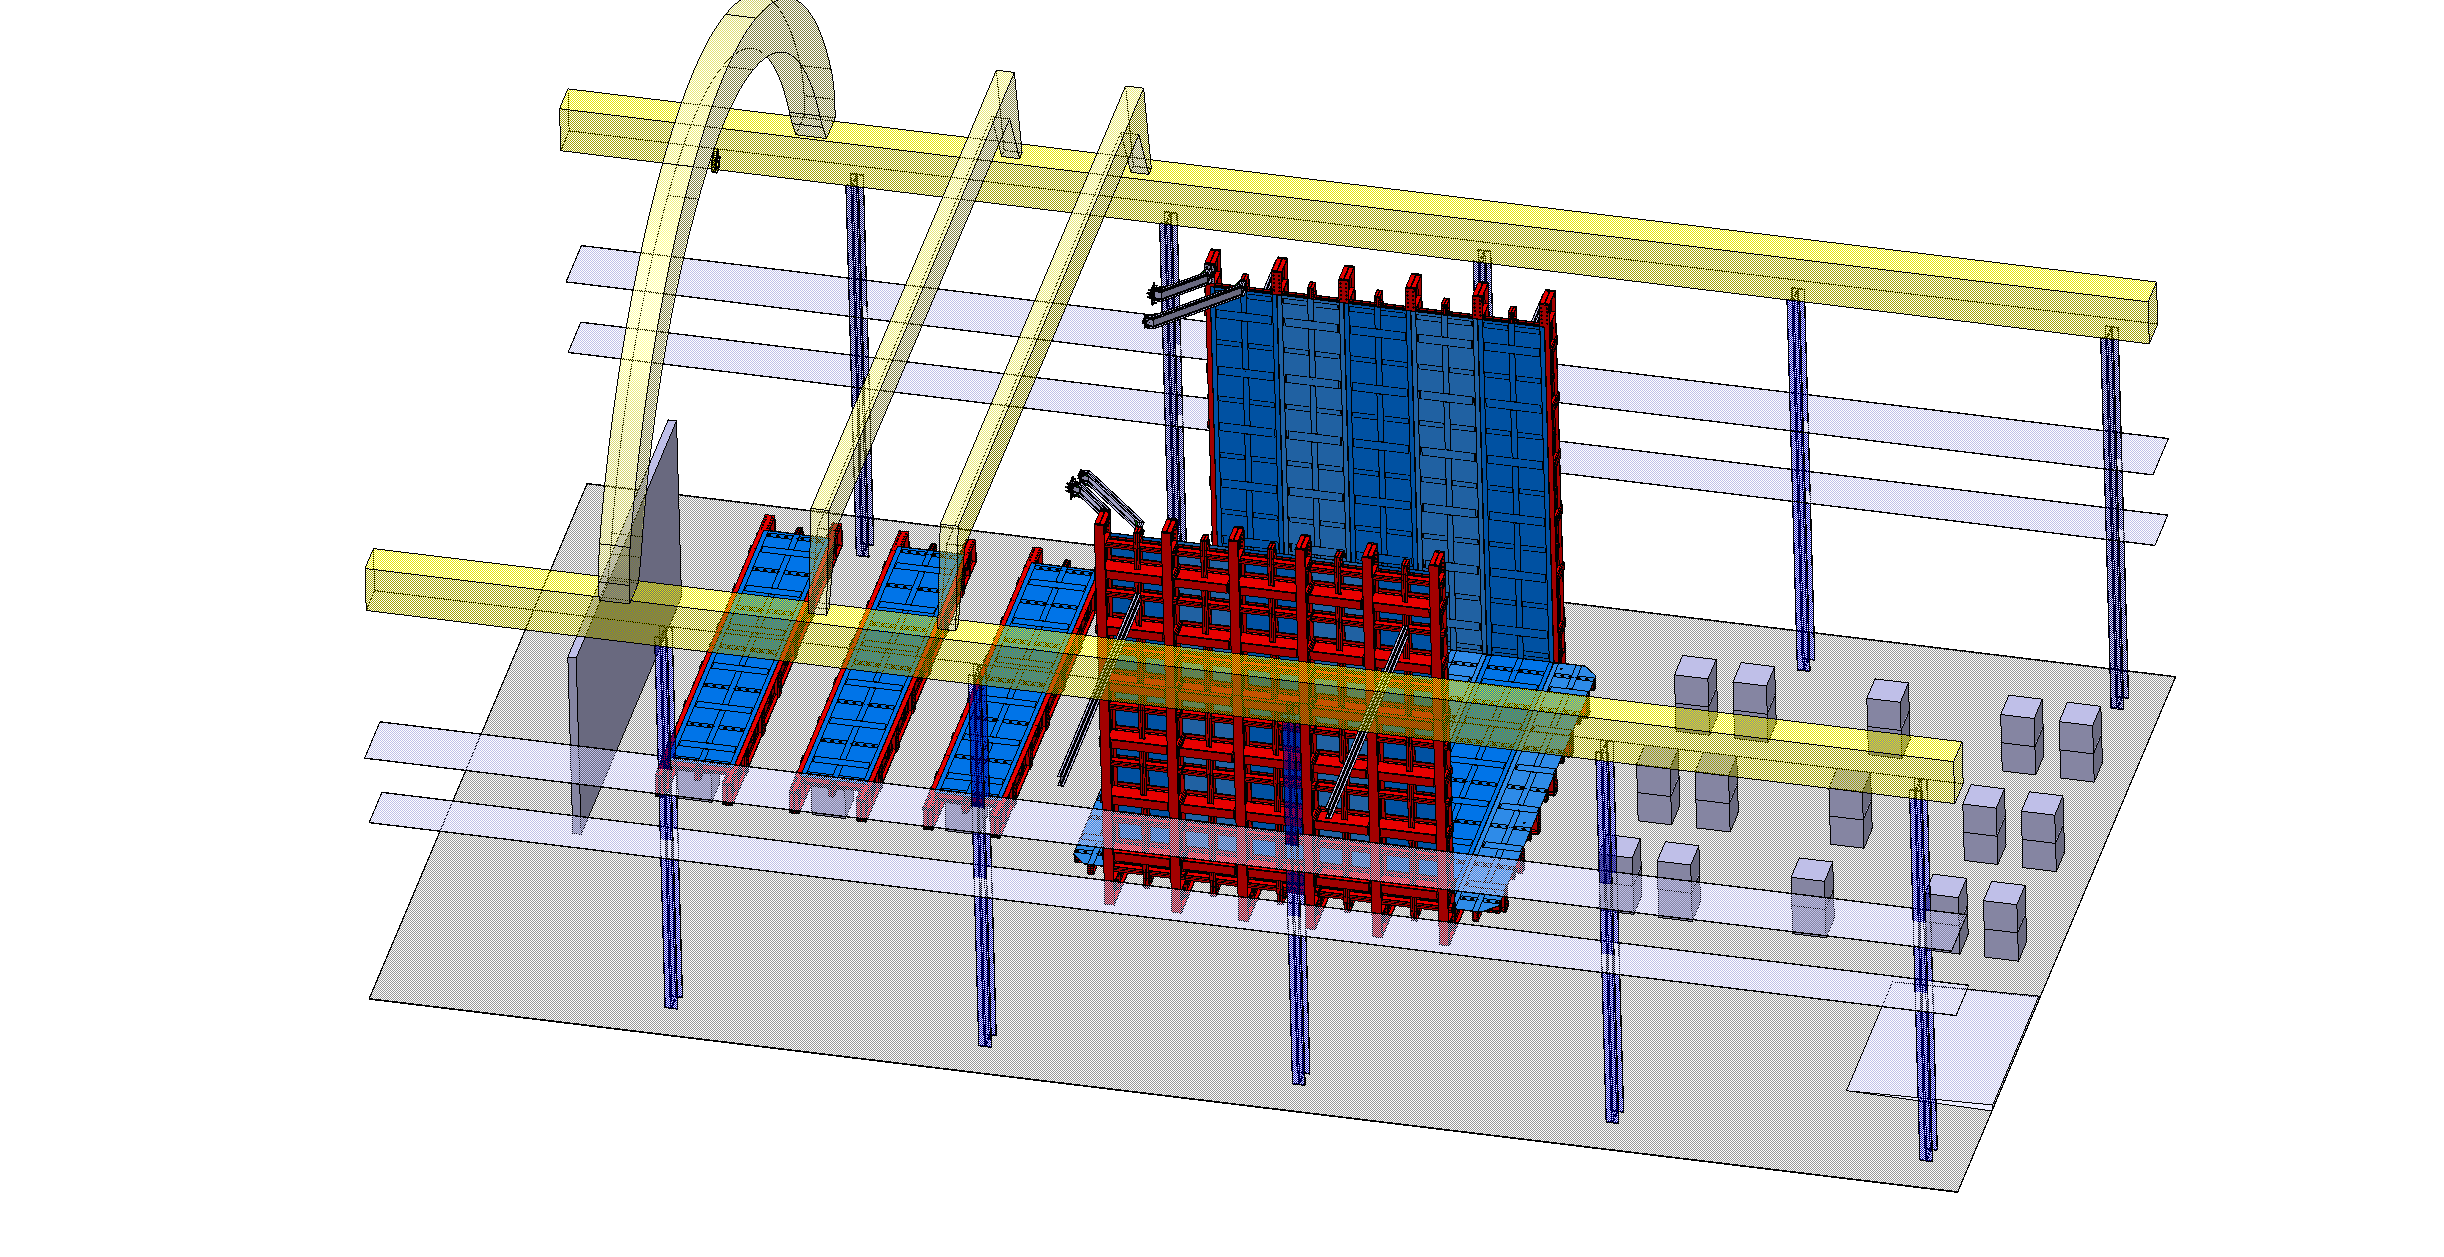
\includegraphics[width=0.32\textwidth]{./Figures/assembly_sequence_11_07/21.png}}
\subfigure[]{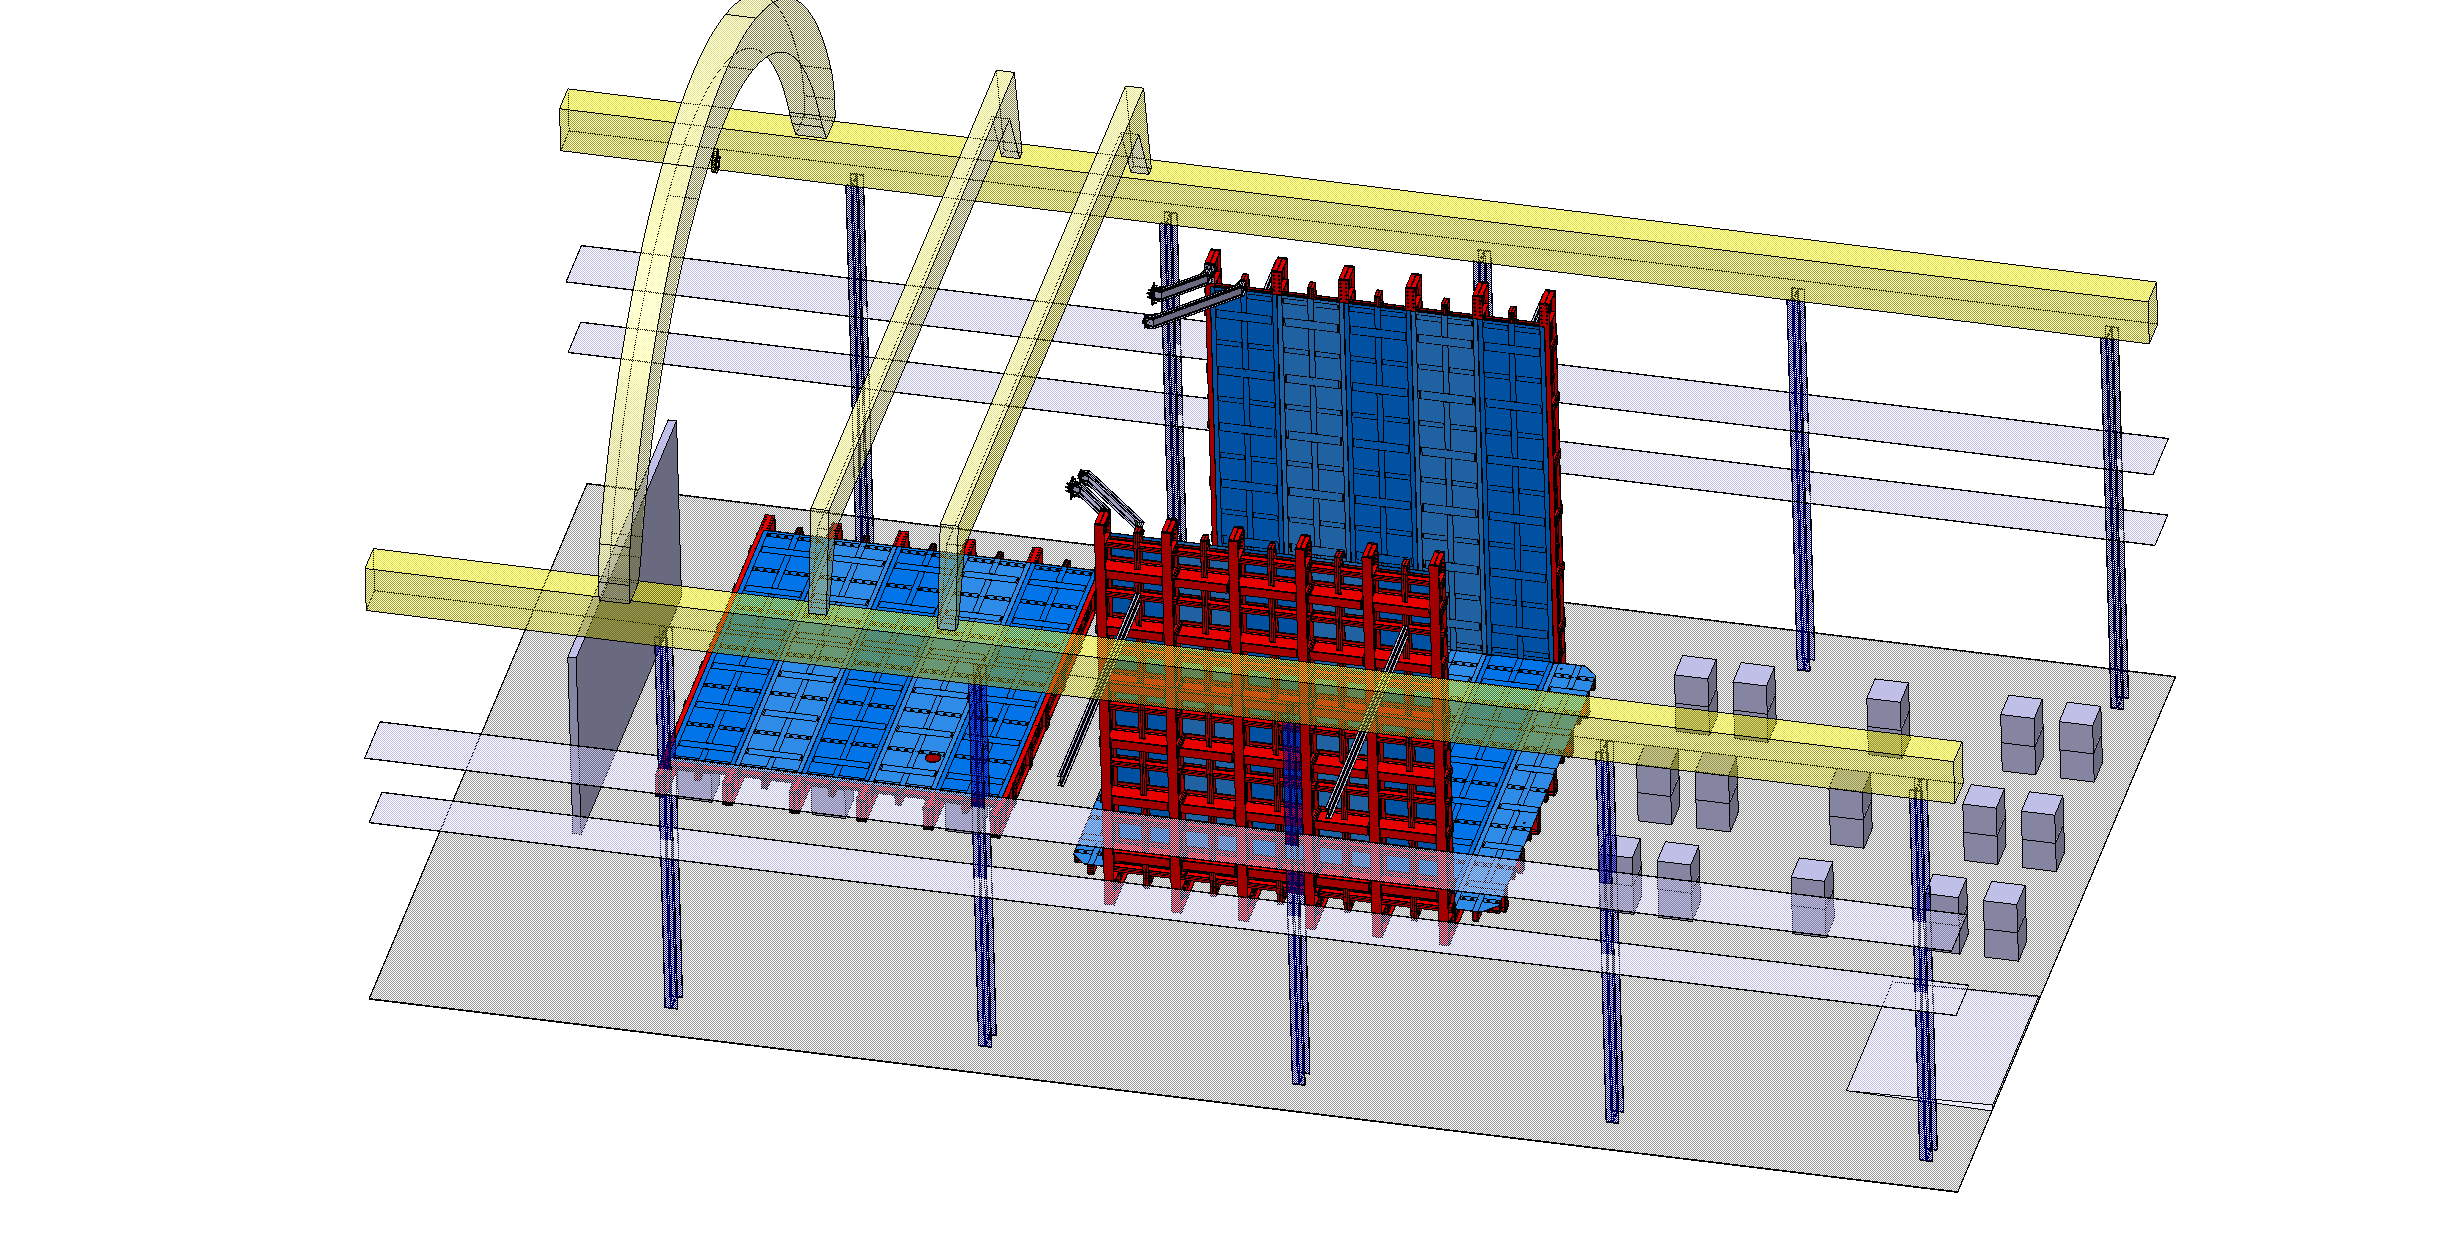
\includegraphics[width=0.32\textwidth]{./Figures/assembly_sequence_11_07/22.png}}
\subfigure[]{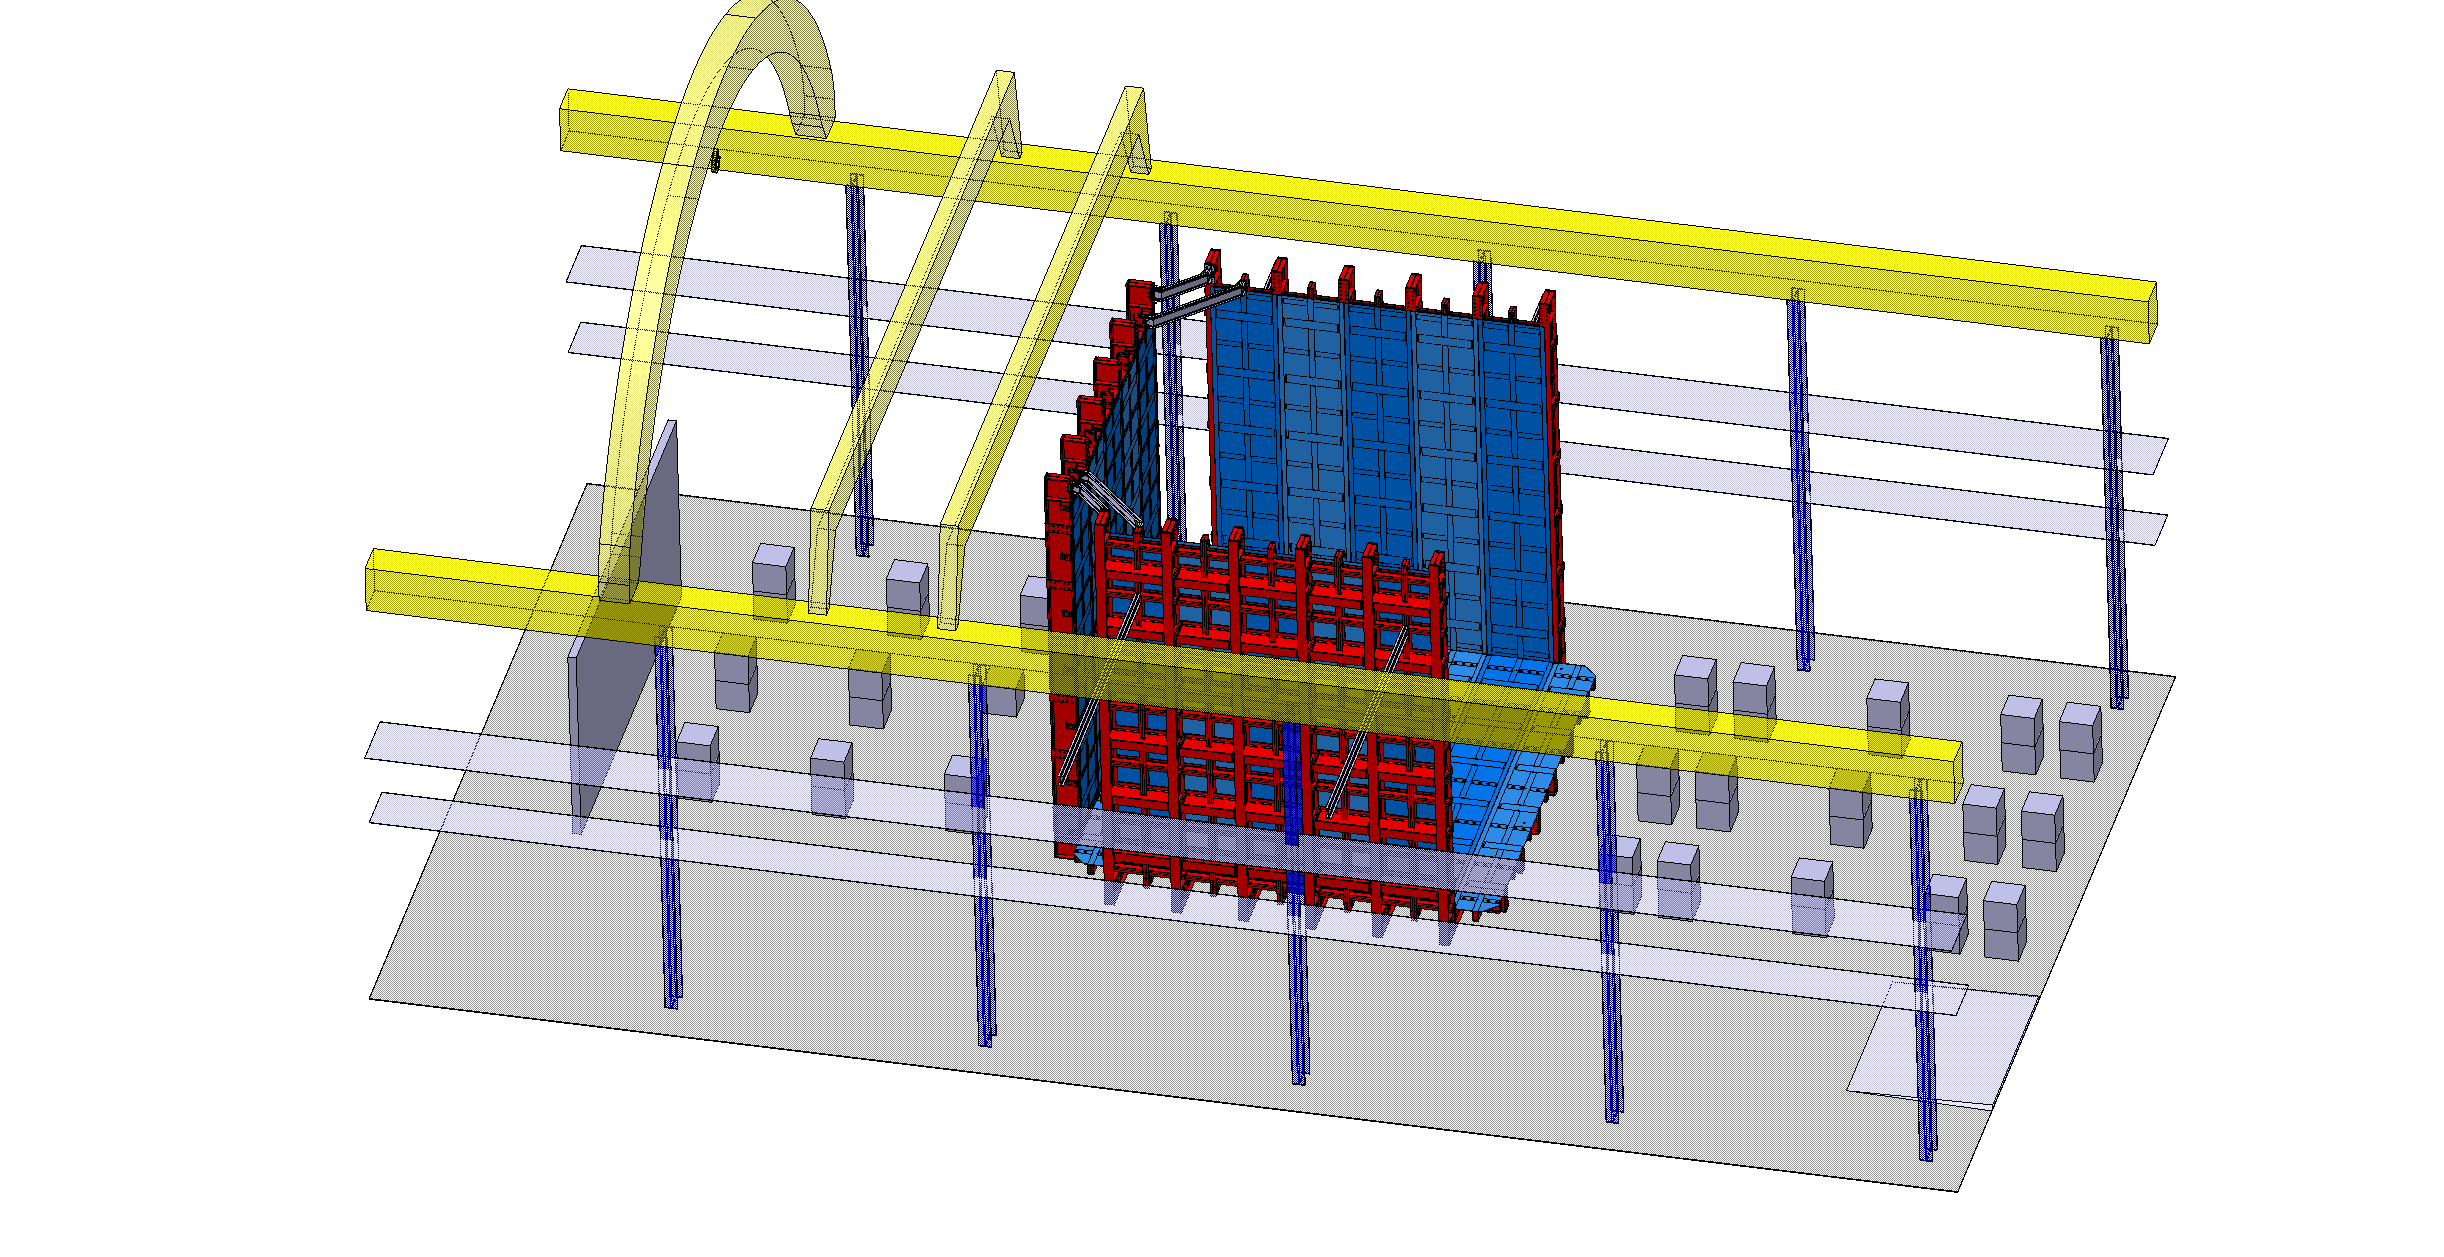
\includegraphics[width=0.32\textwidth]{./Figures/assembly_sequence_11_07/23.png}}
\subfigure[]{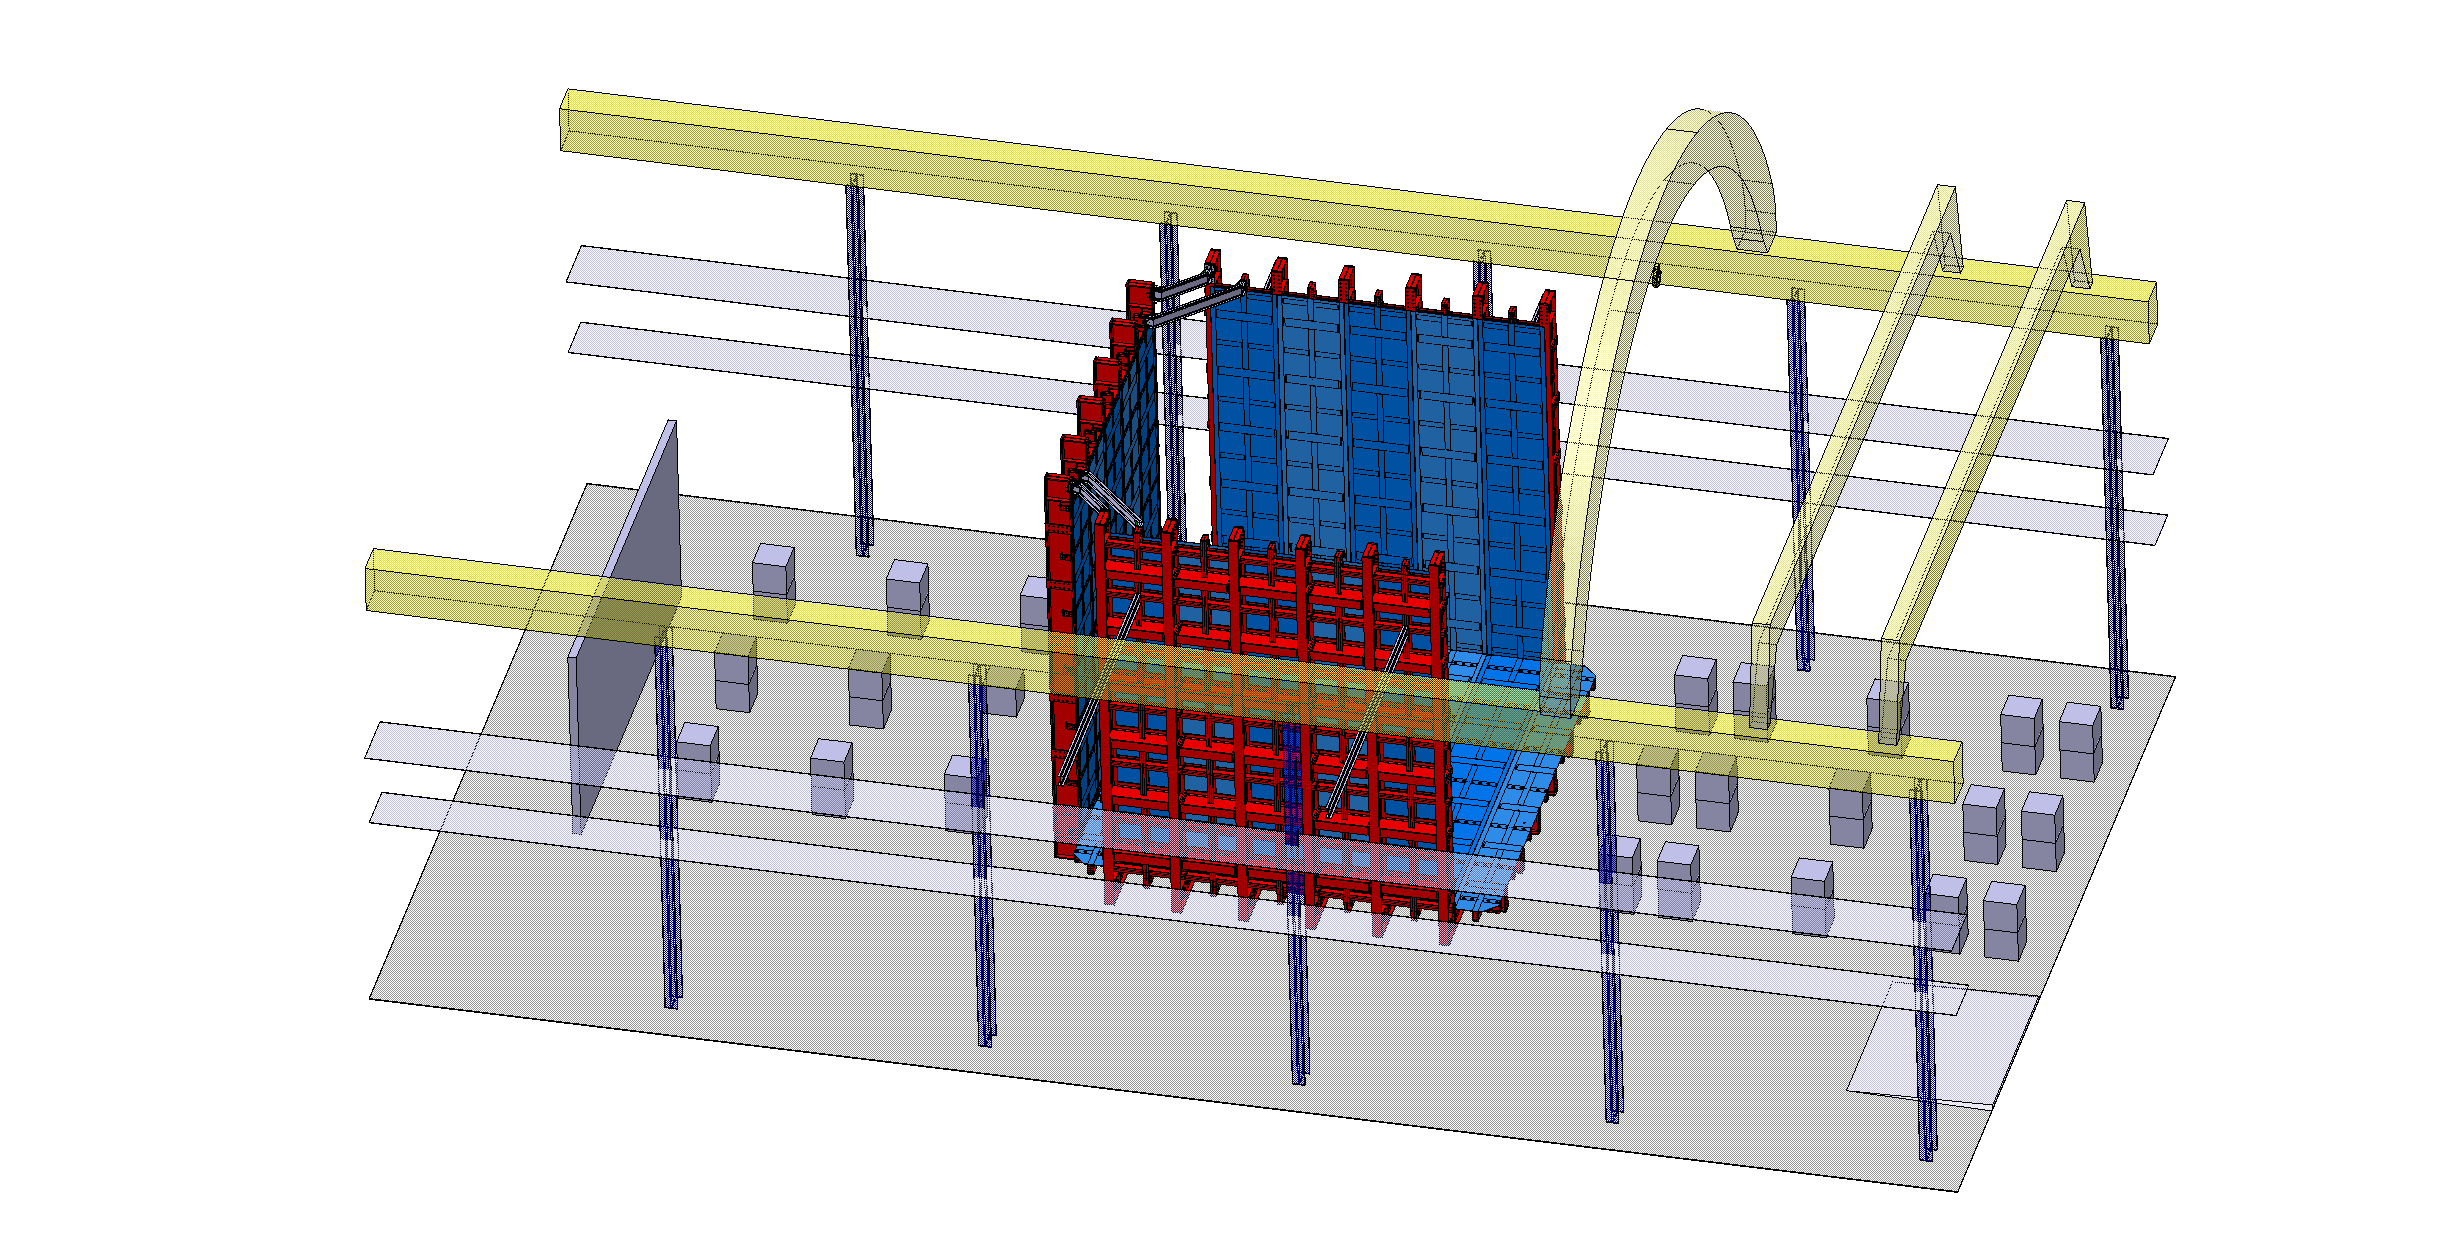
\includegraphics[width=0.32\textwidth]{./Figures/assembly_sequence_11_07/24.png}}
\subfigure[]{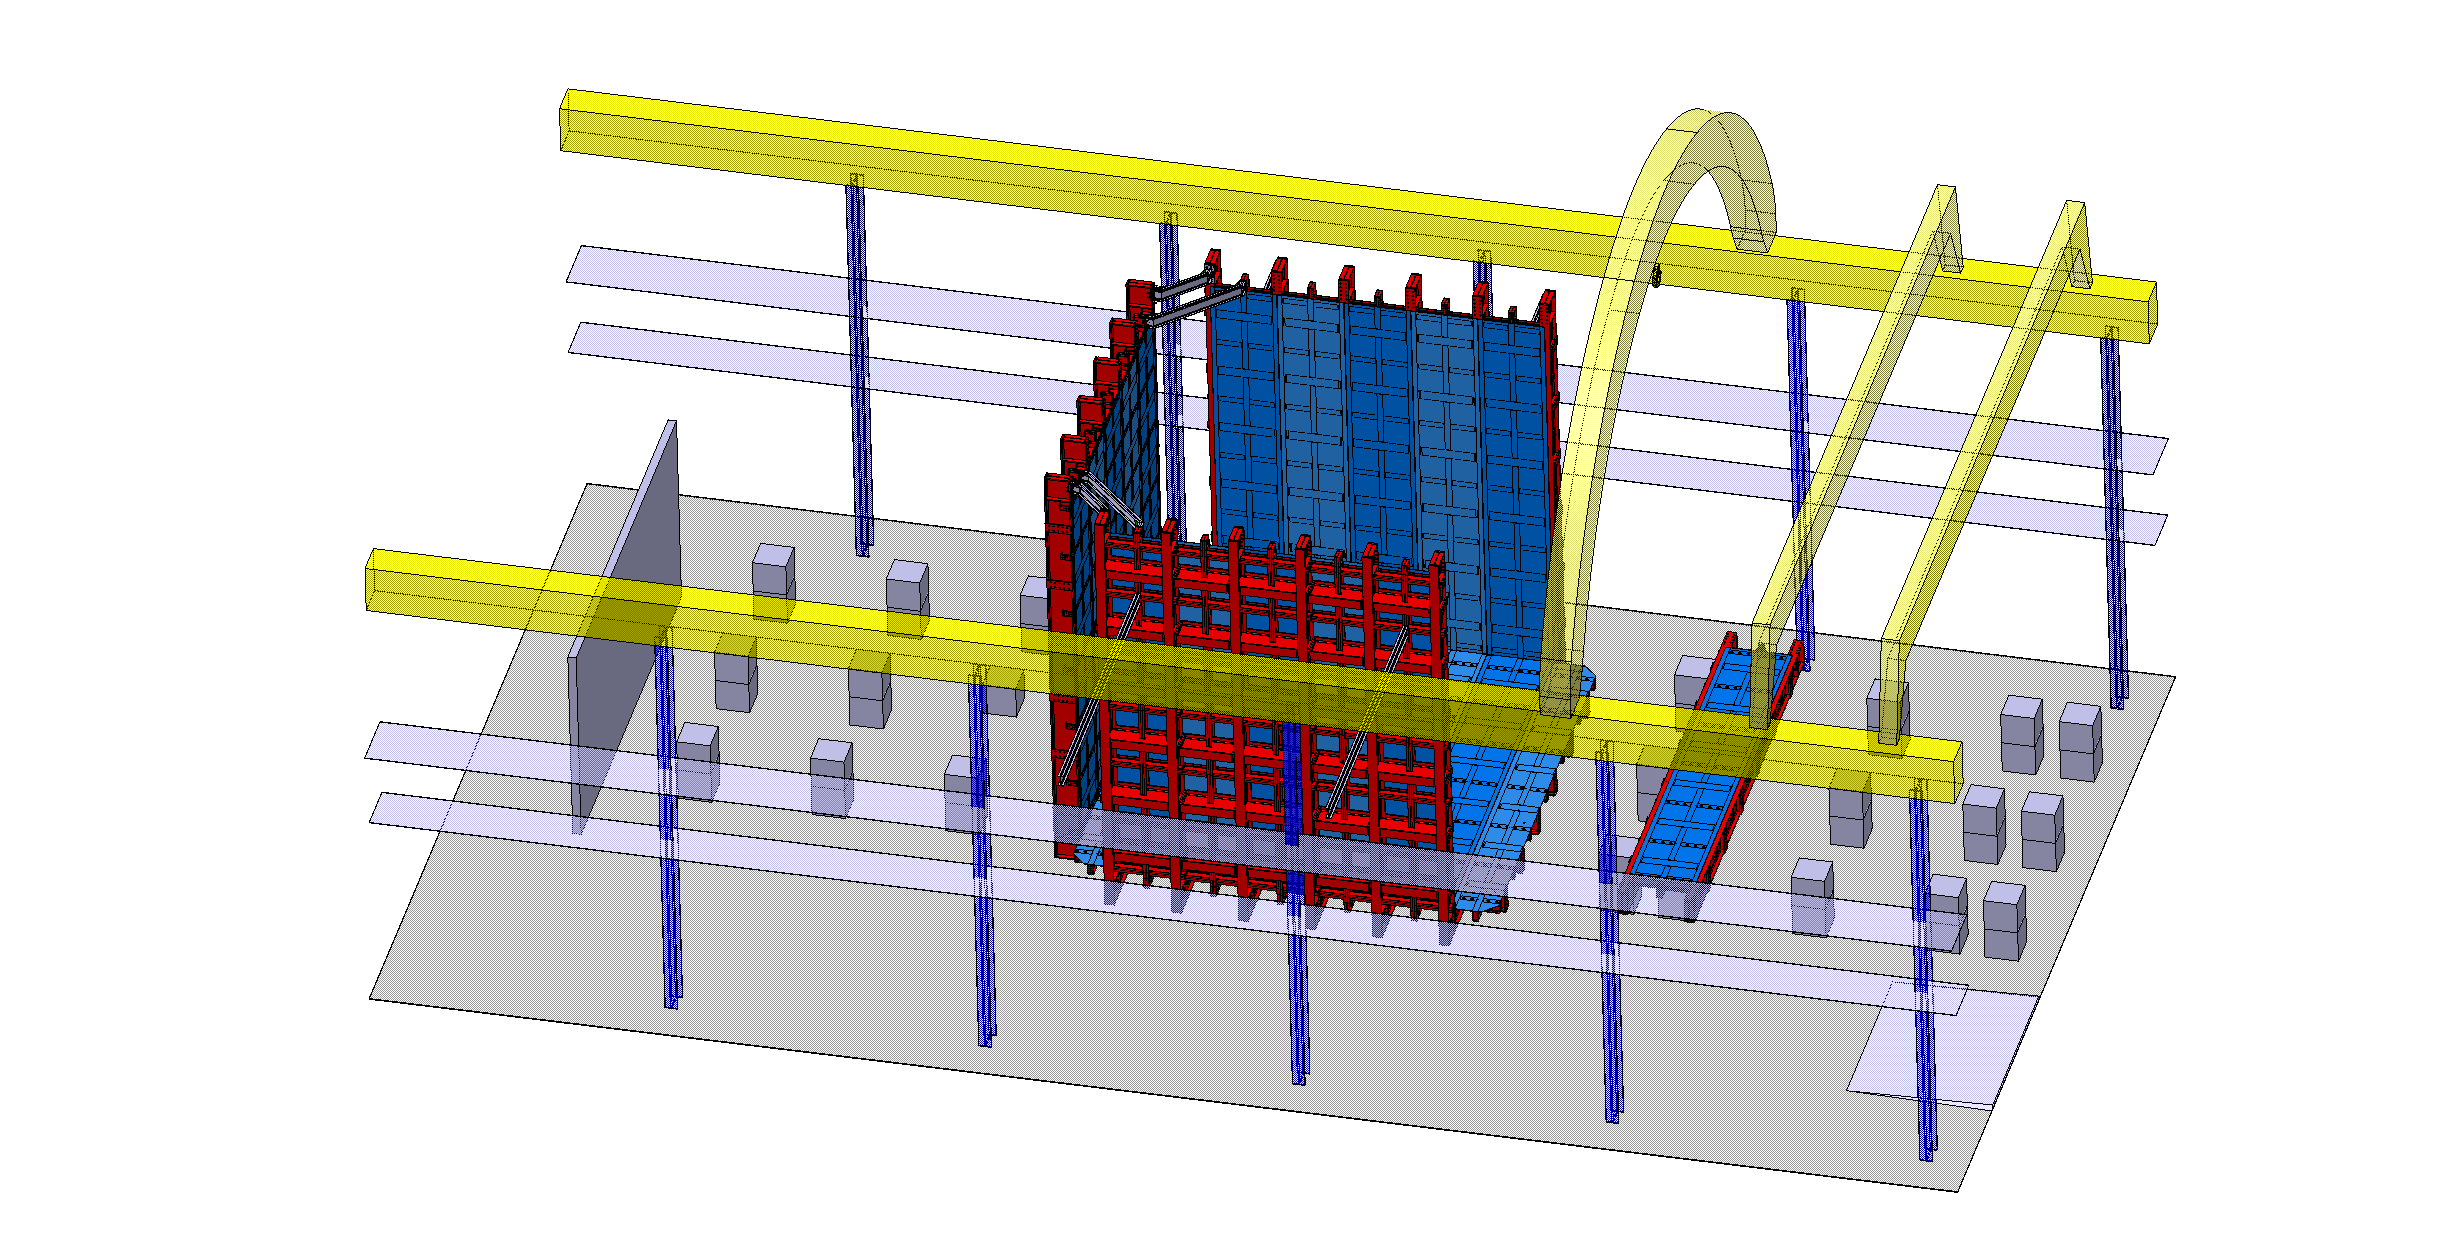
\includegraphics[width=0.32\textwidth]{./Figures/assembly_sequence_11_07/25.png}}
\subfigure[]{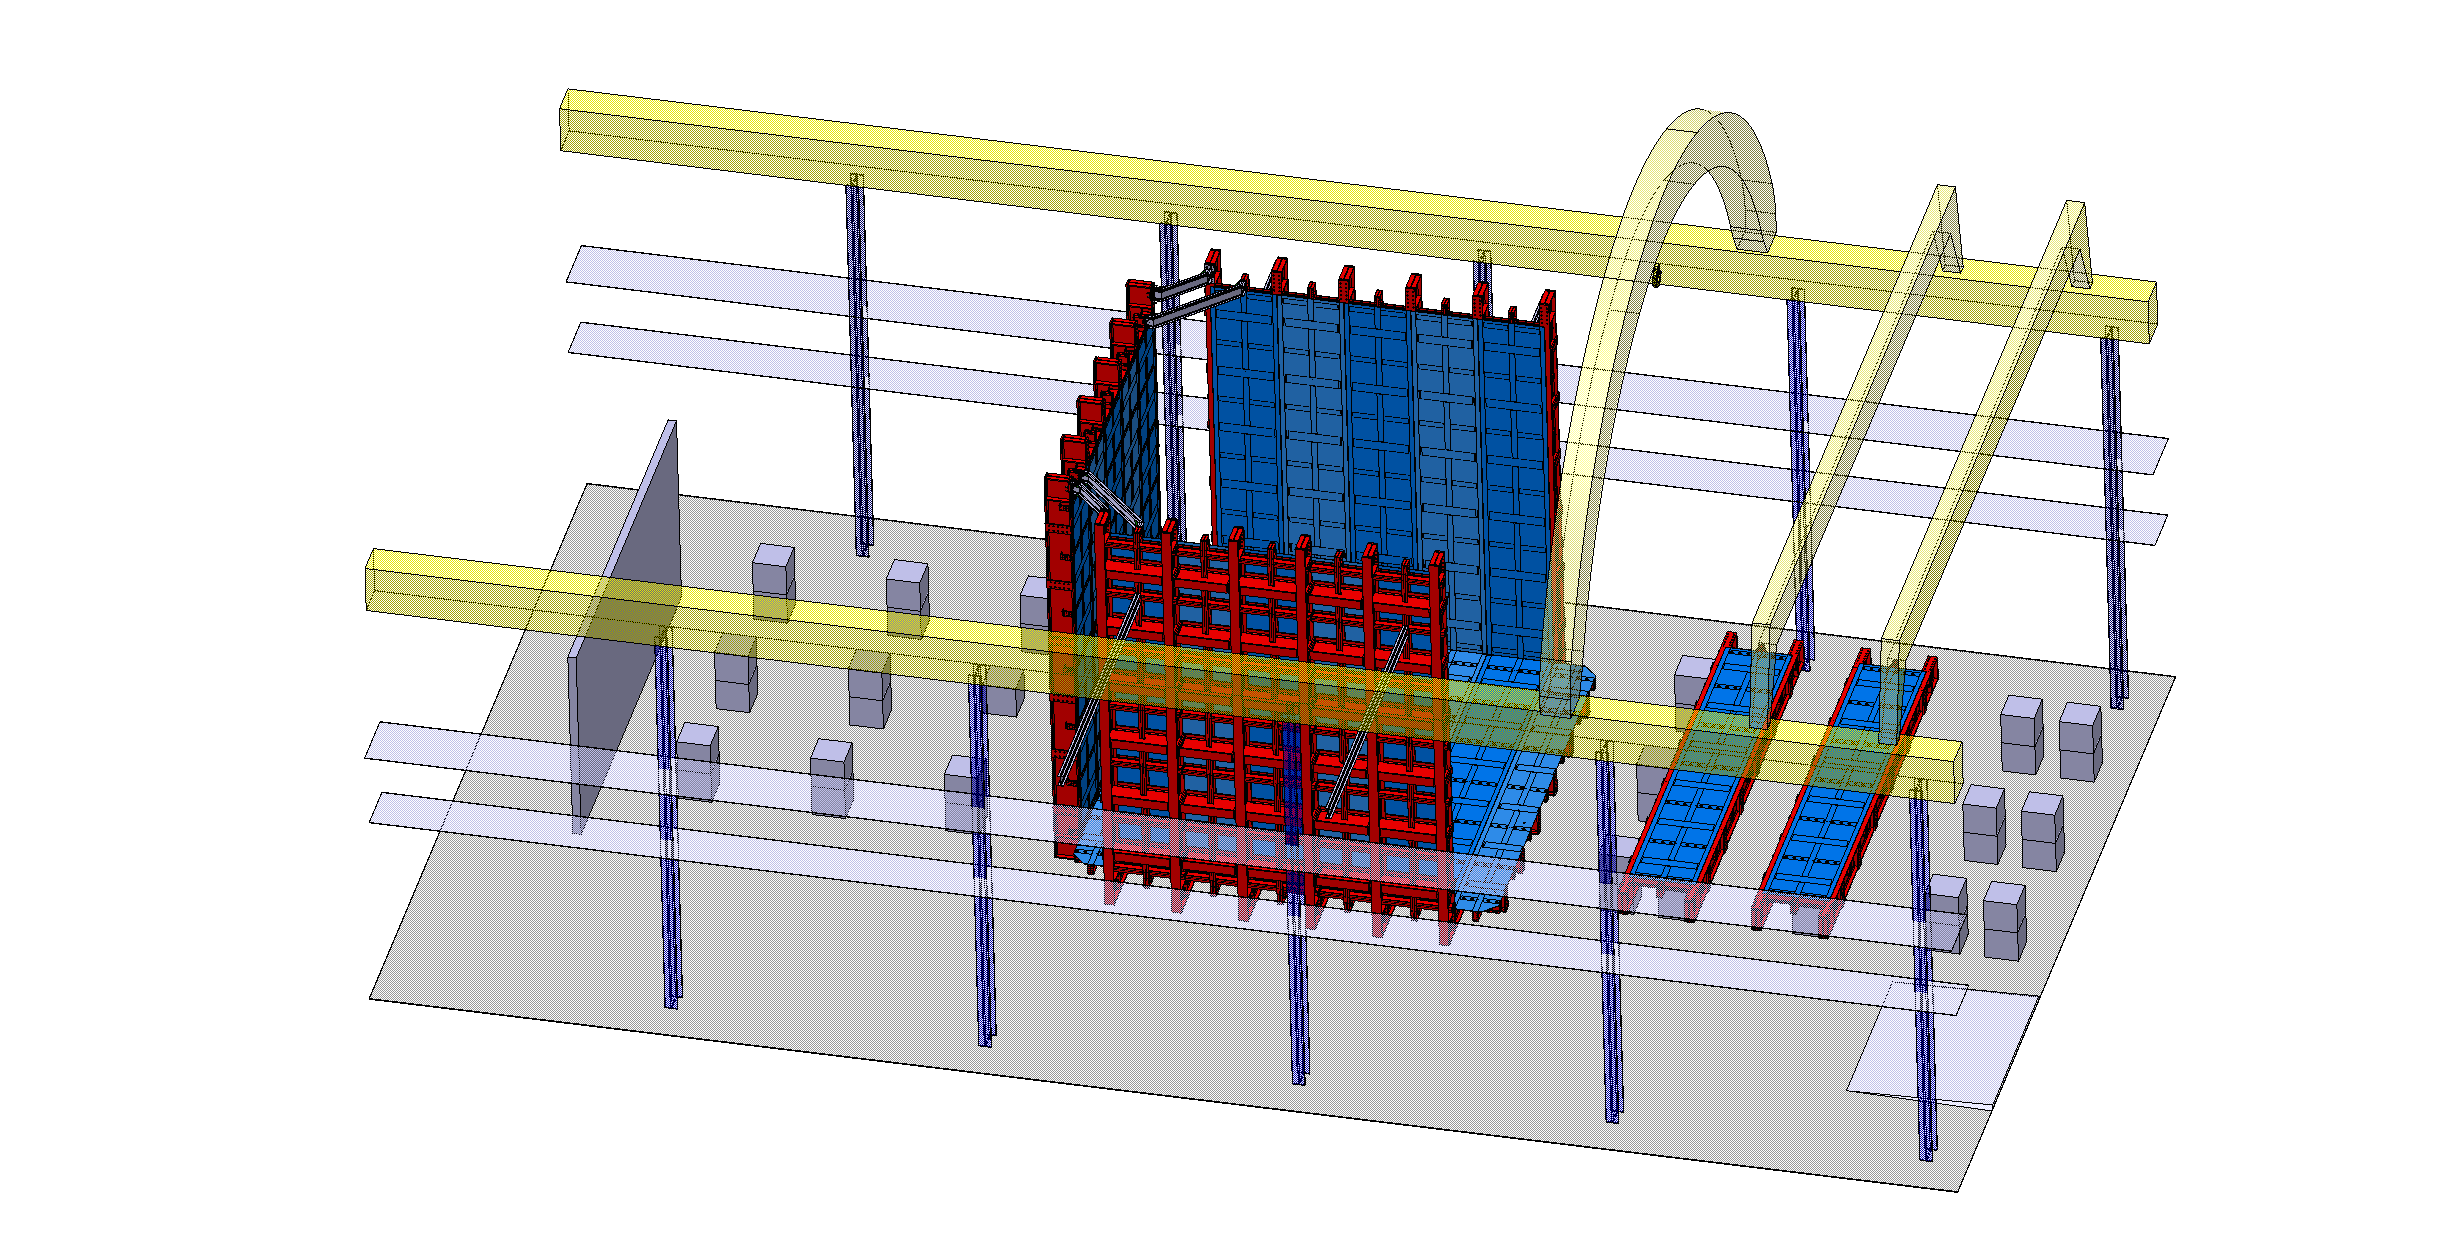
\includegraphics[width=0.32\textwidth]{./Figures/assembly_sequence_11_07/26.png}}
\subfigure[]{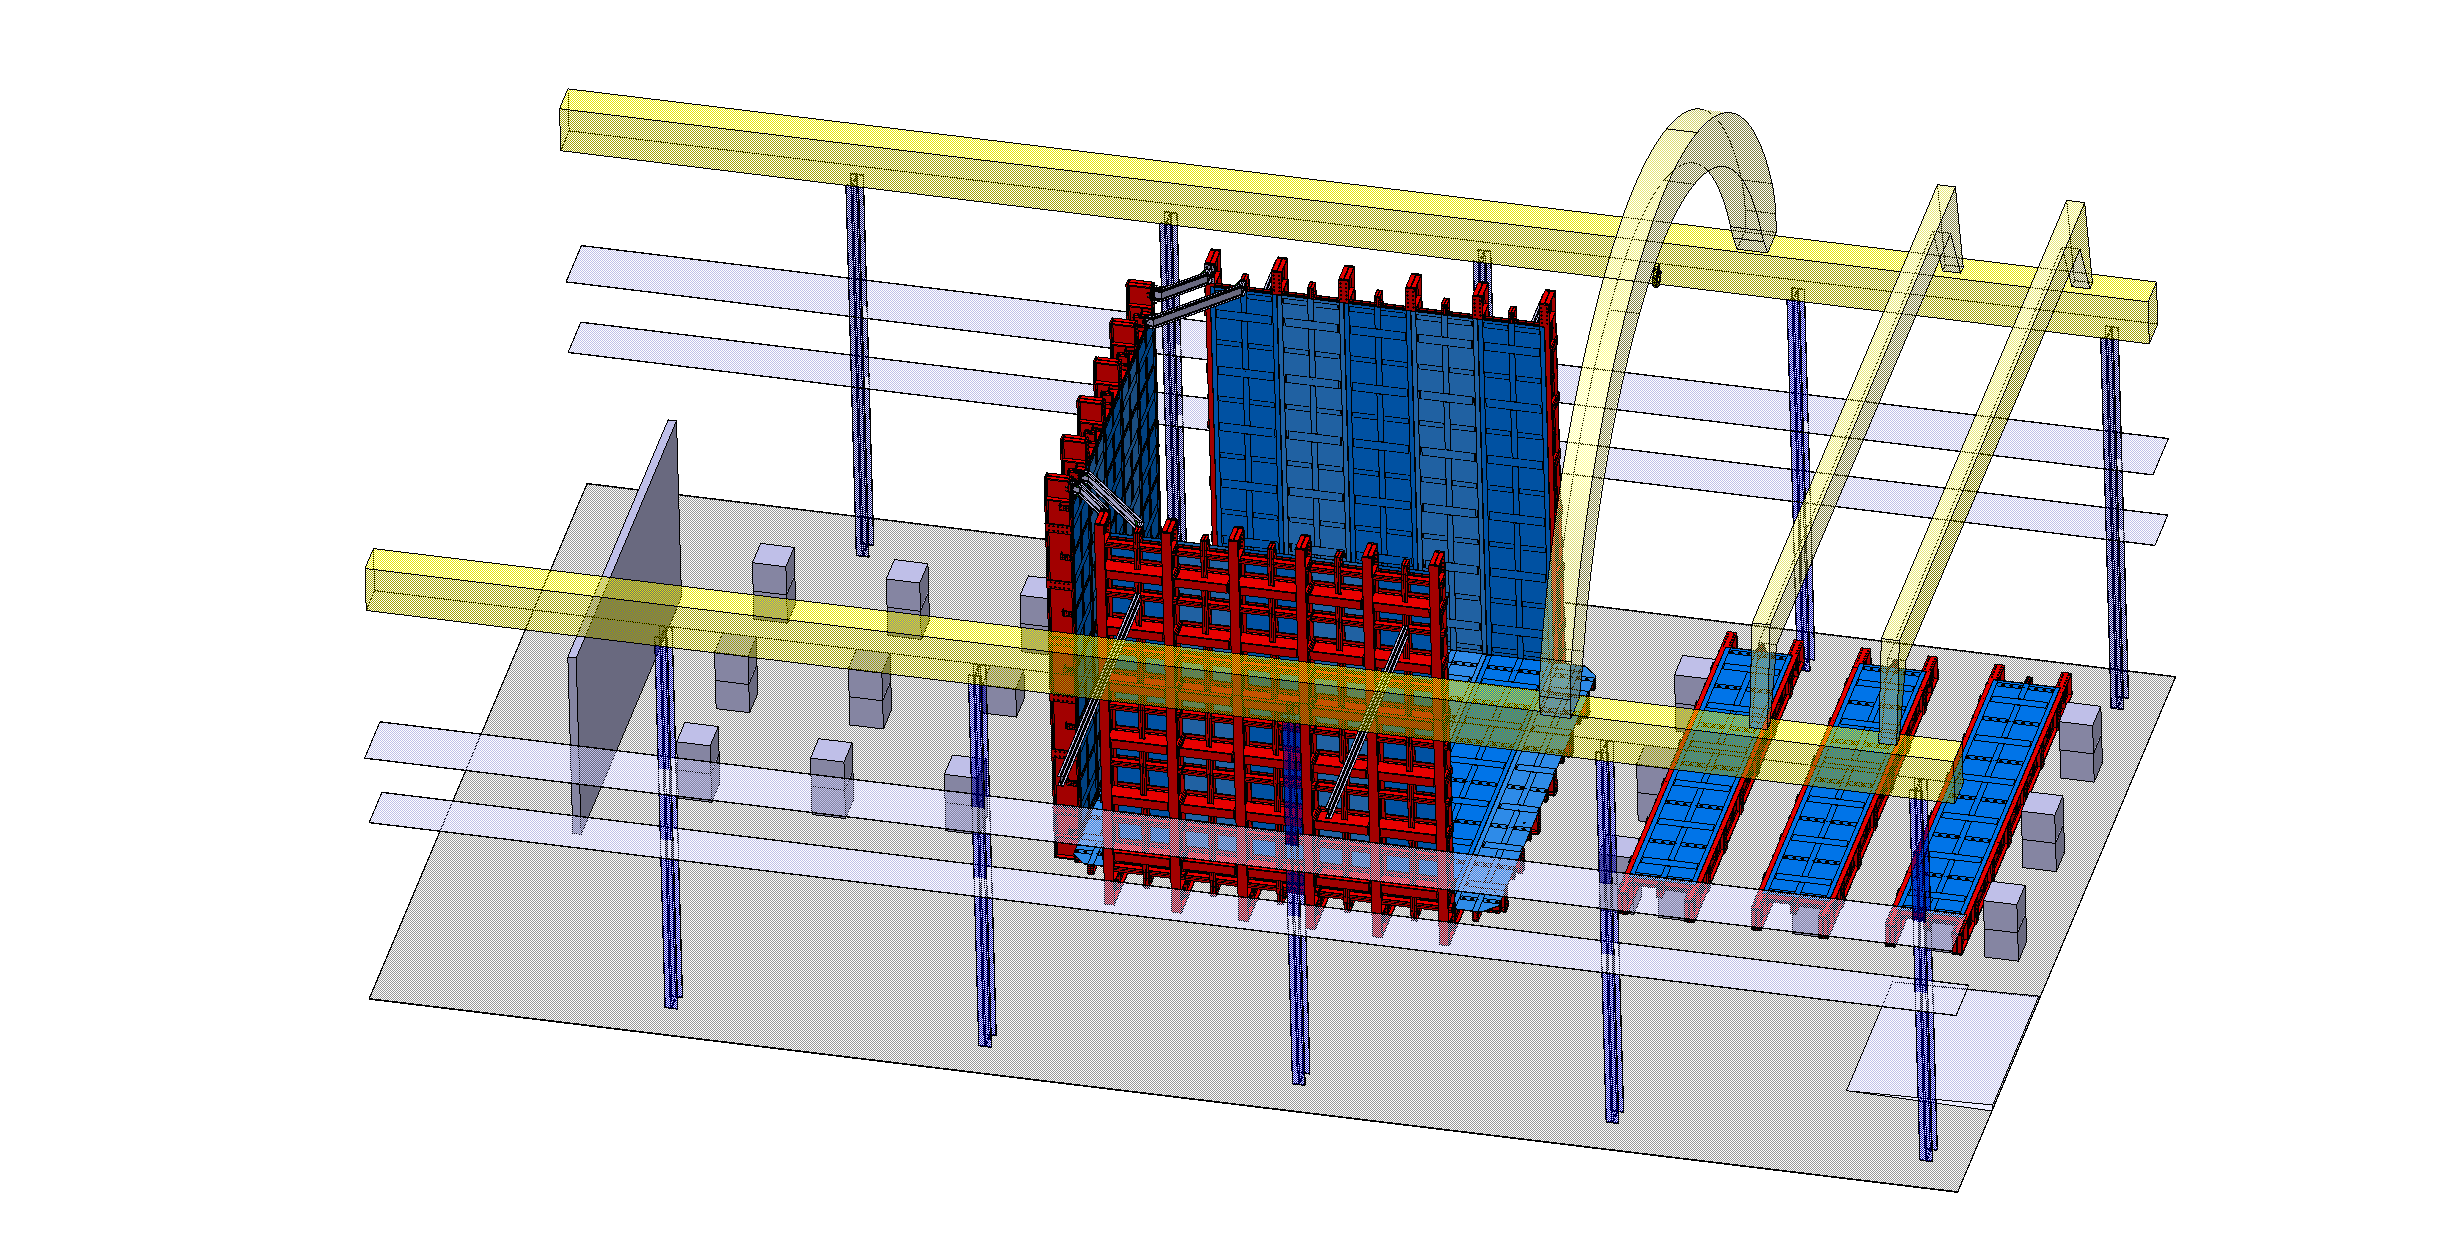
\includegraphics[width=0.32\textwidth]{./Figures/assembly_sequence_11_07/27.png}}
\subfigure[]{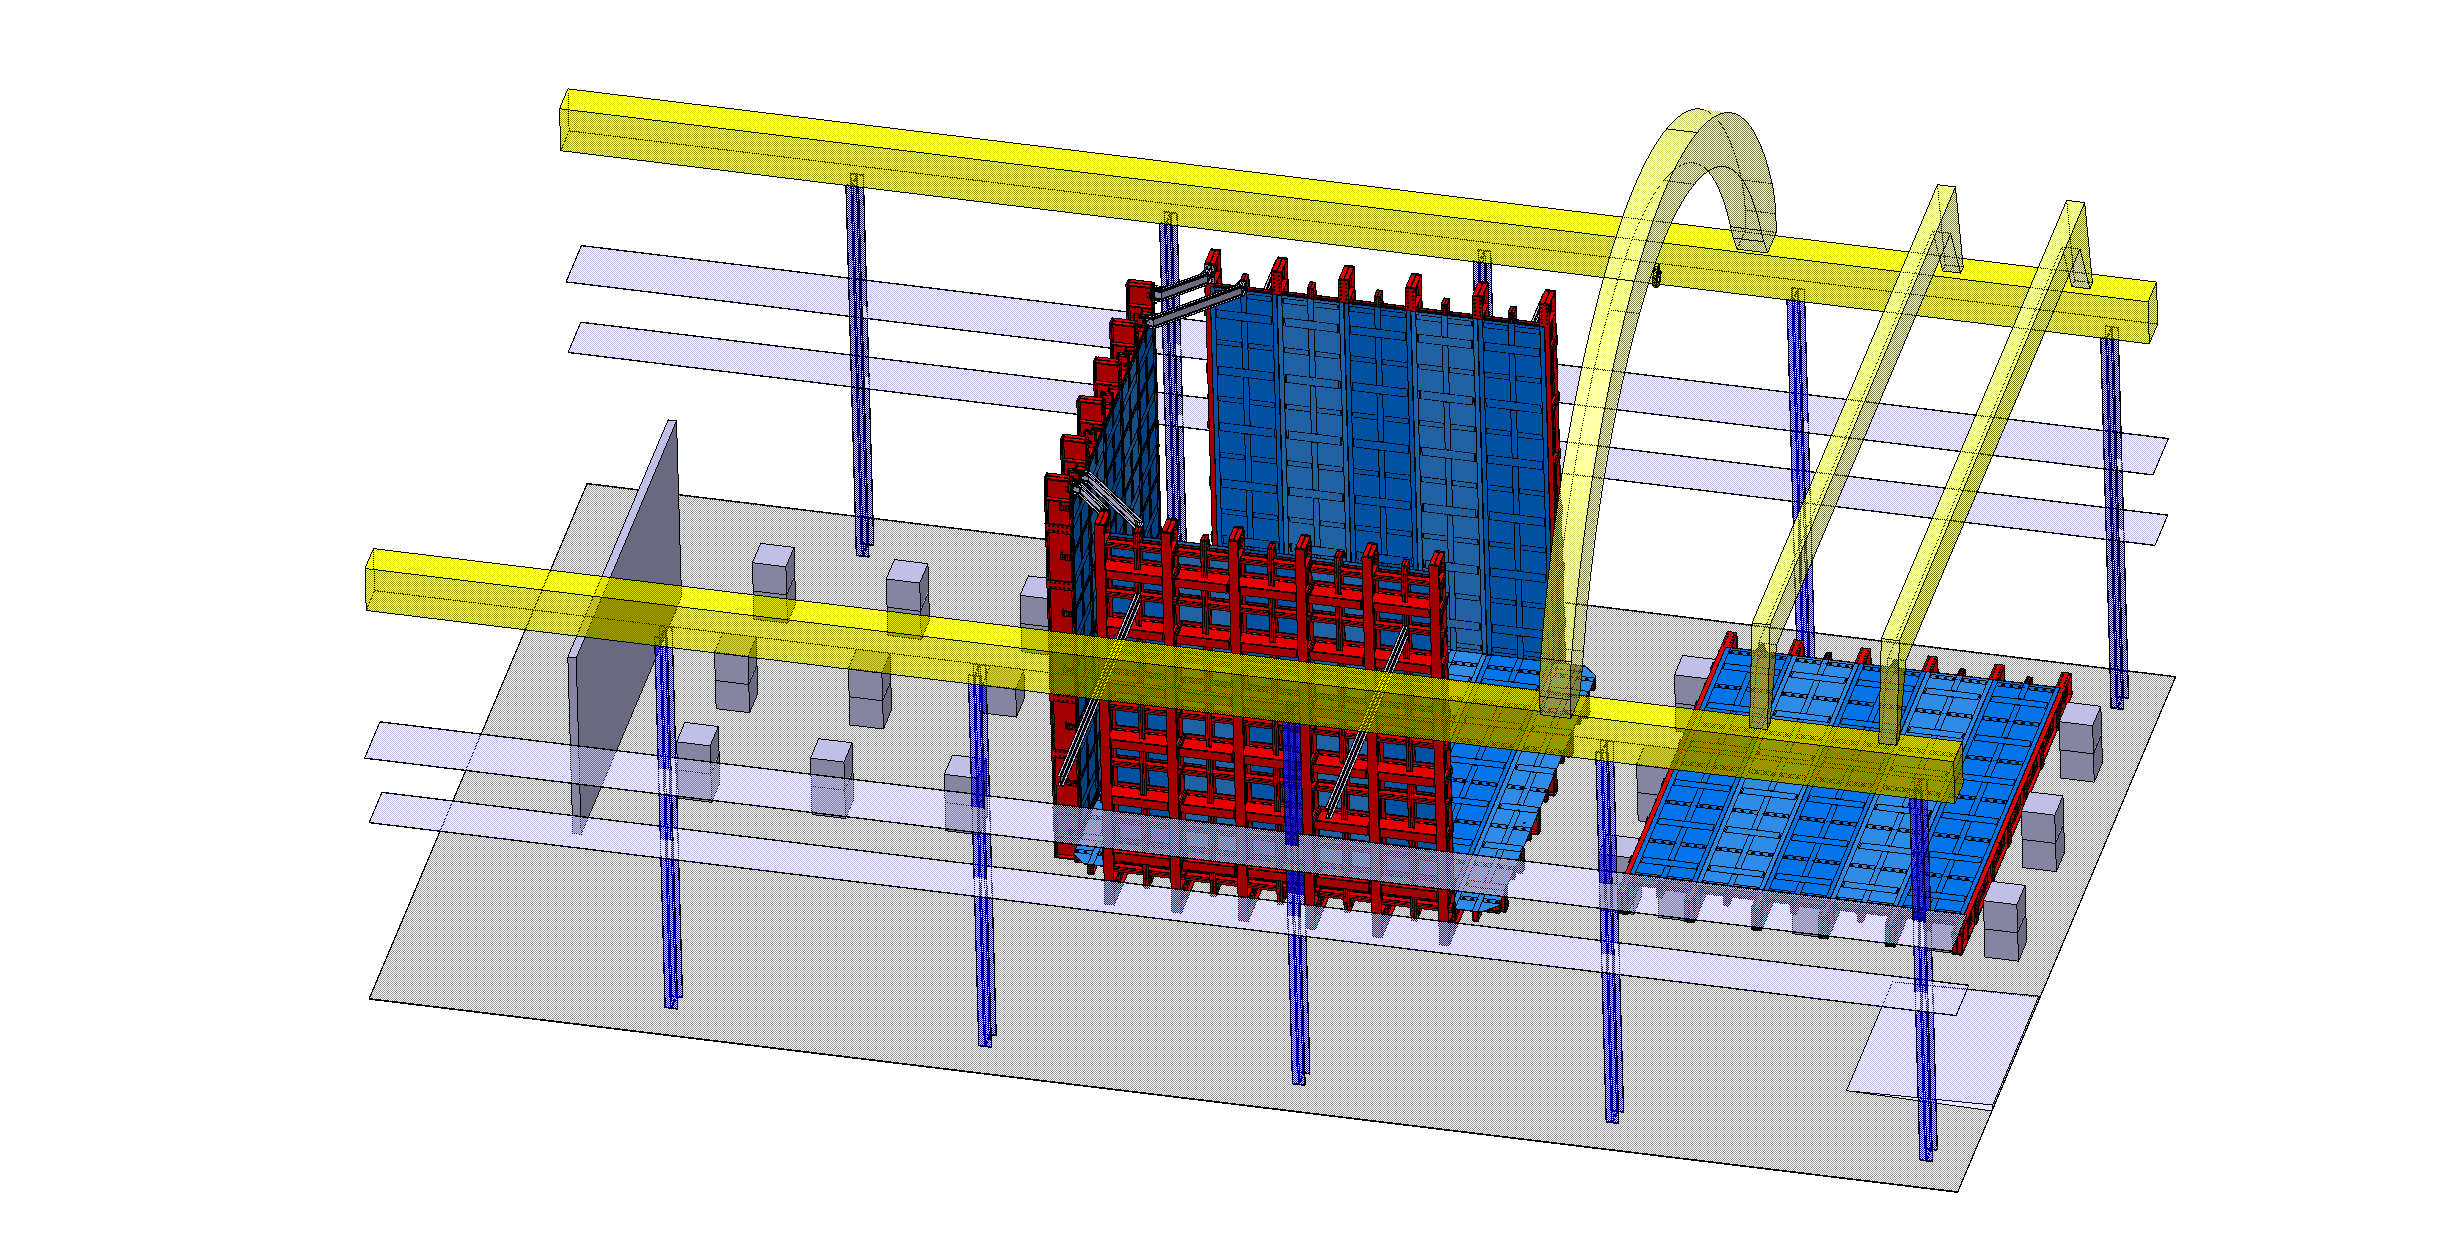
\includegraphics[width=0.32\textwidth]{./Figures/assembly_sequence_11_07/28.png}}
\subfigure[]{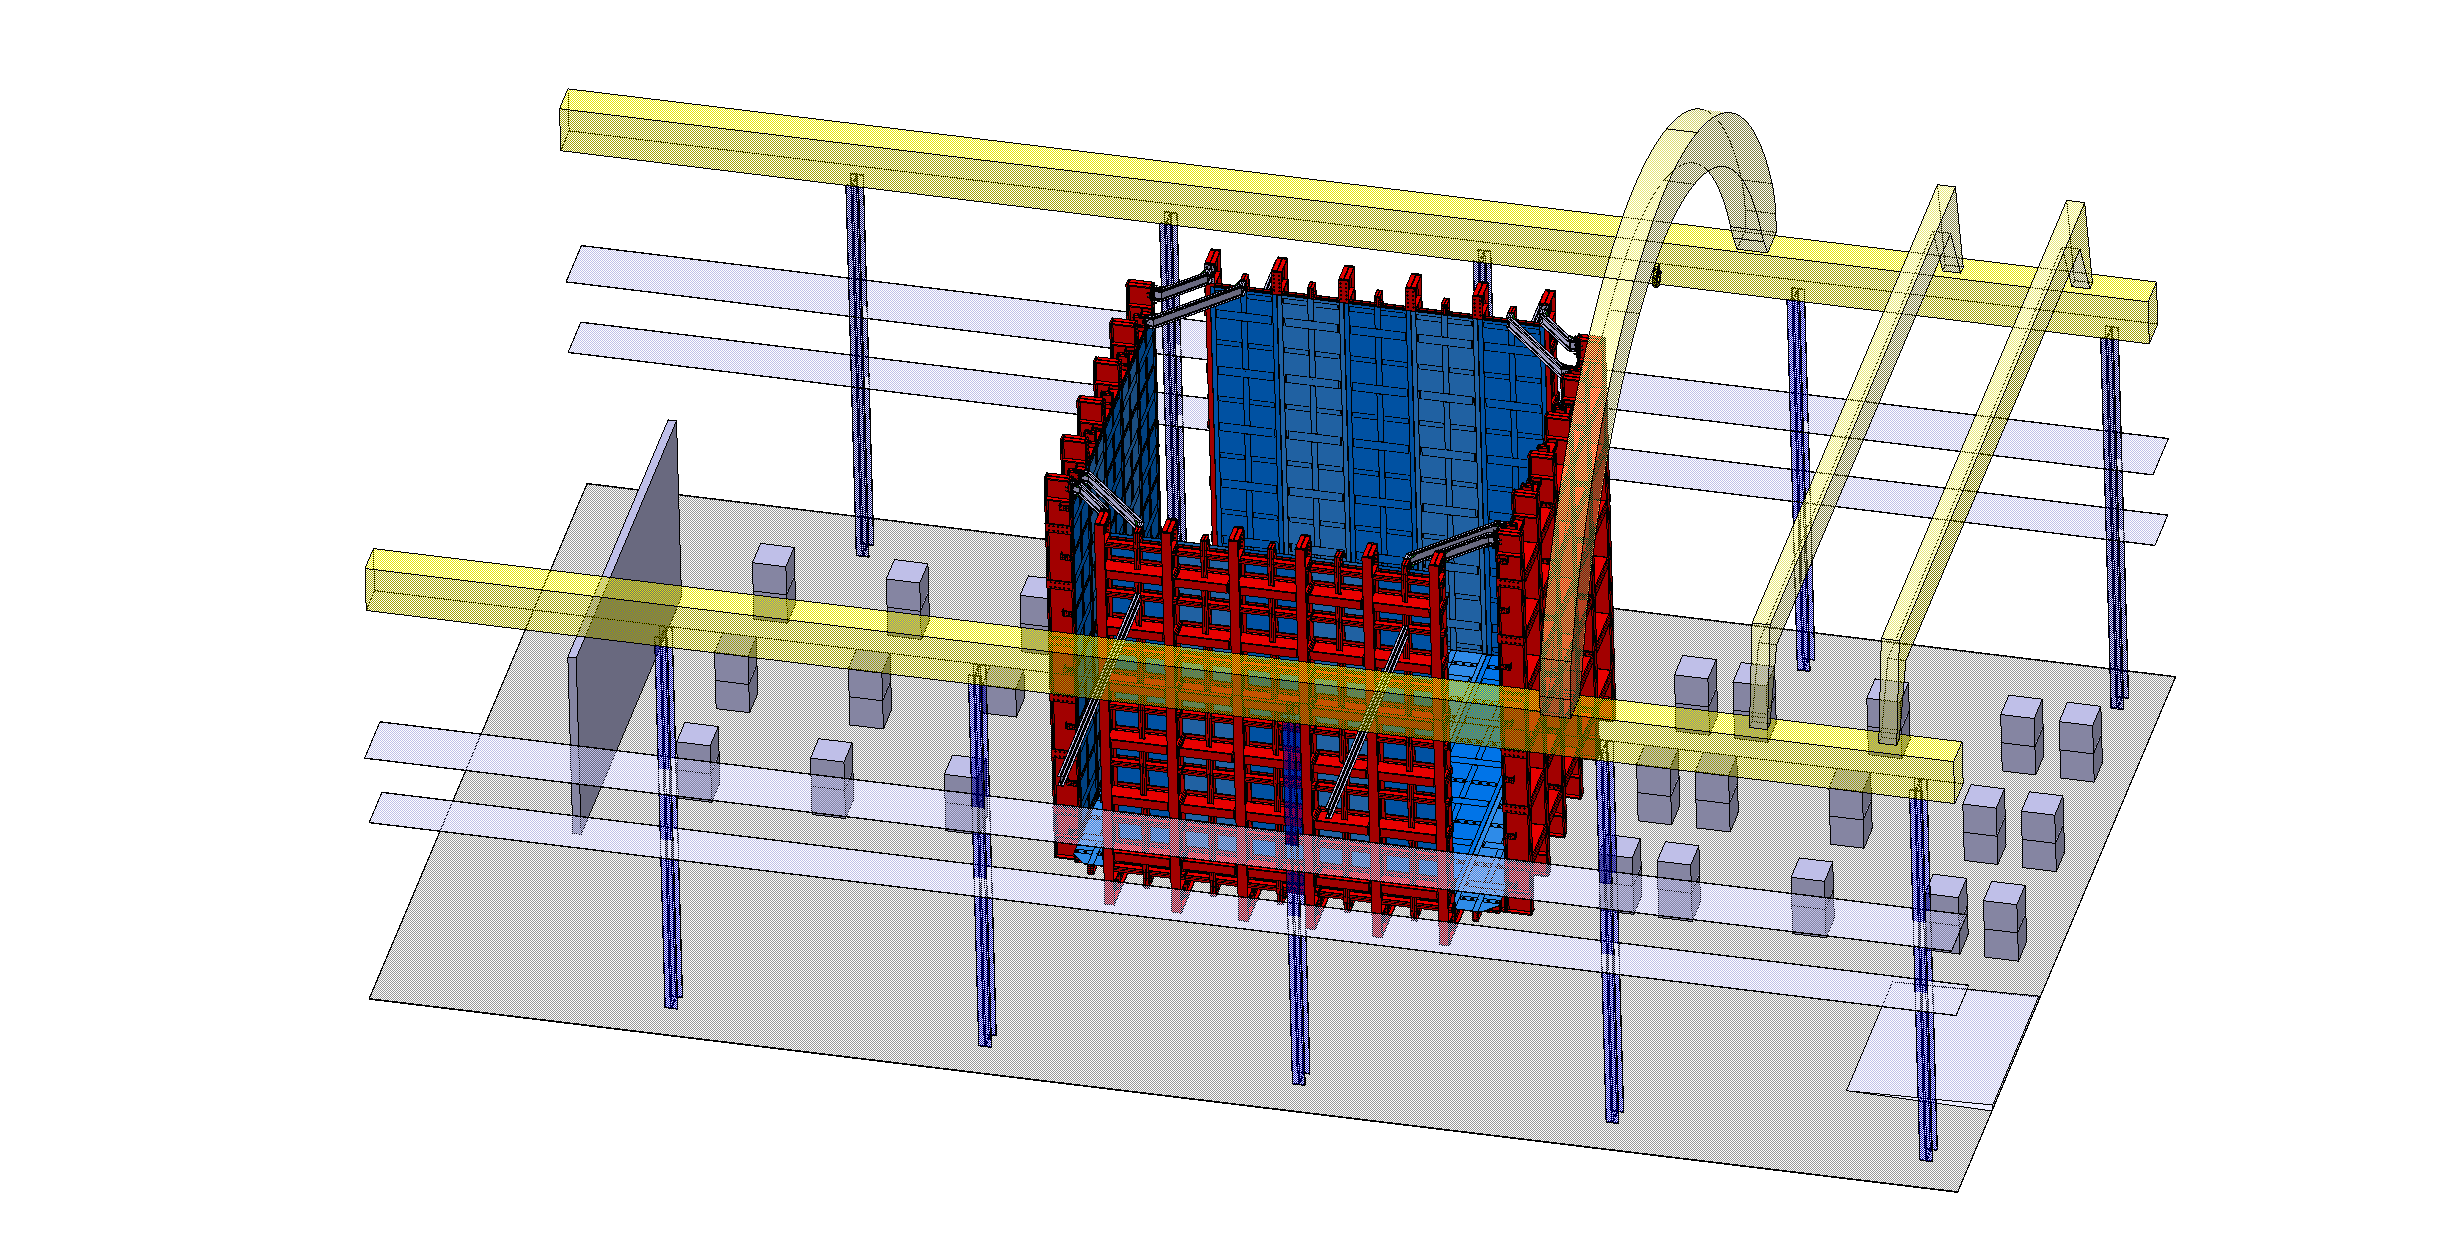
\includegraphics[width=0.32\textwidth]{./Figures/assembly_sequence_11_07/29.png}}
\subfigure[]{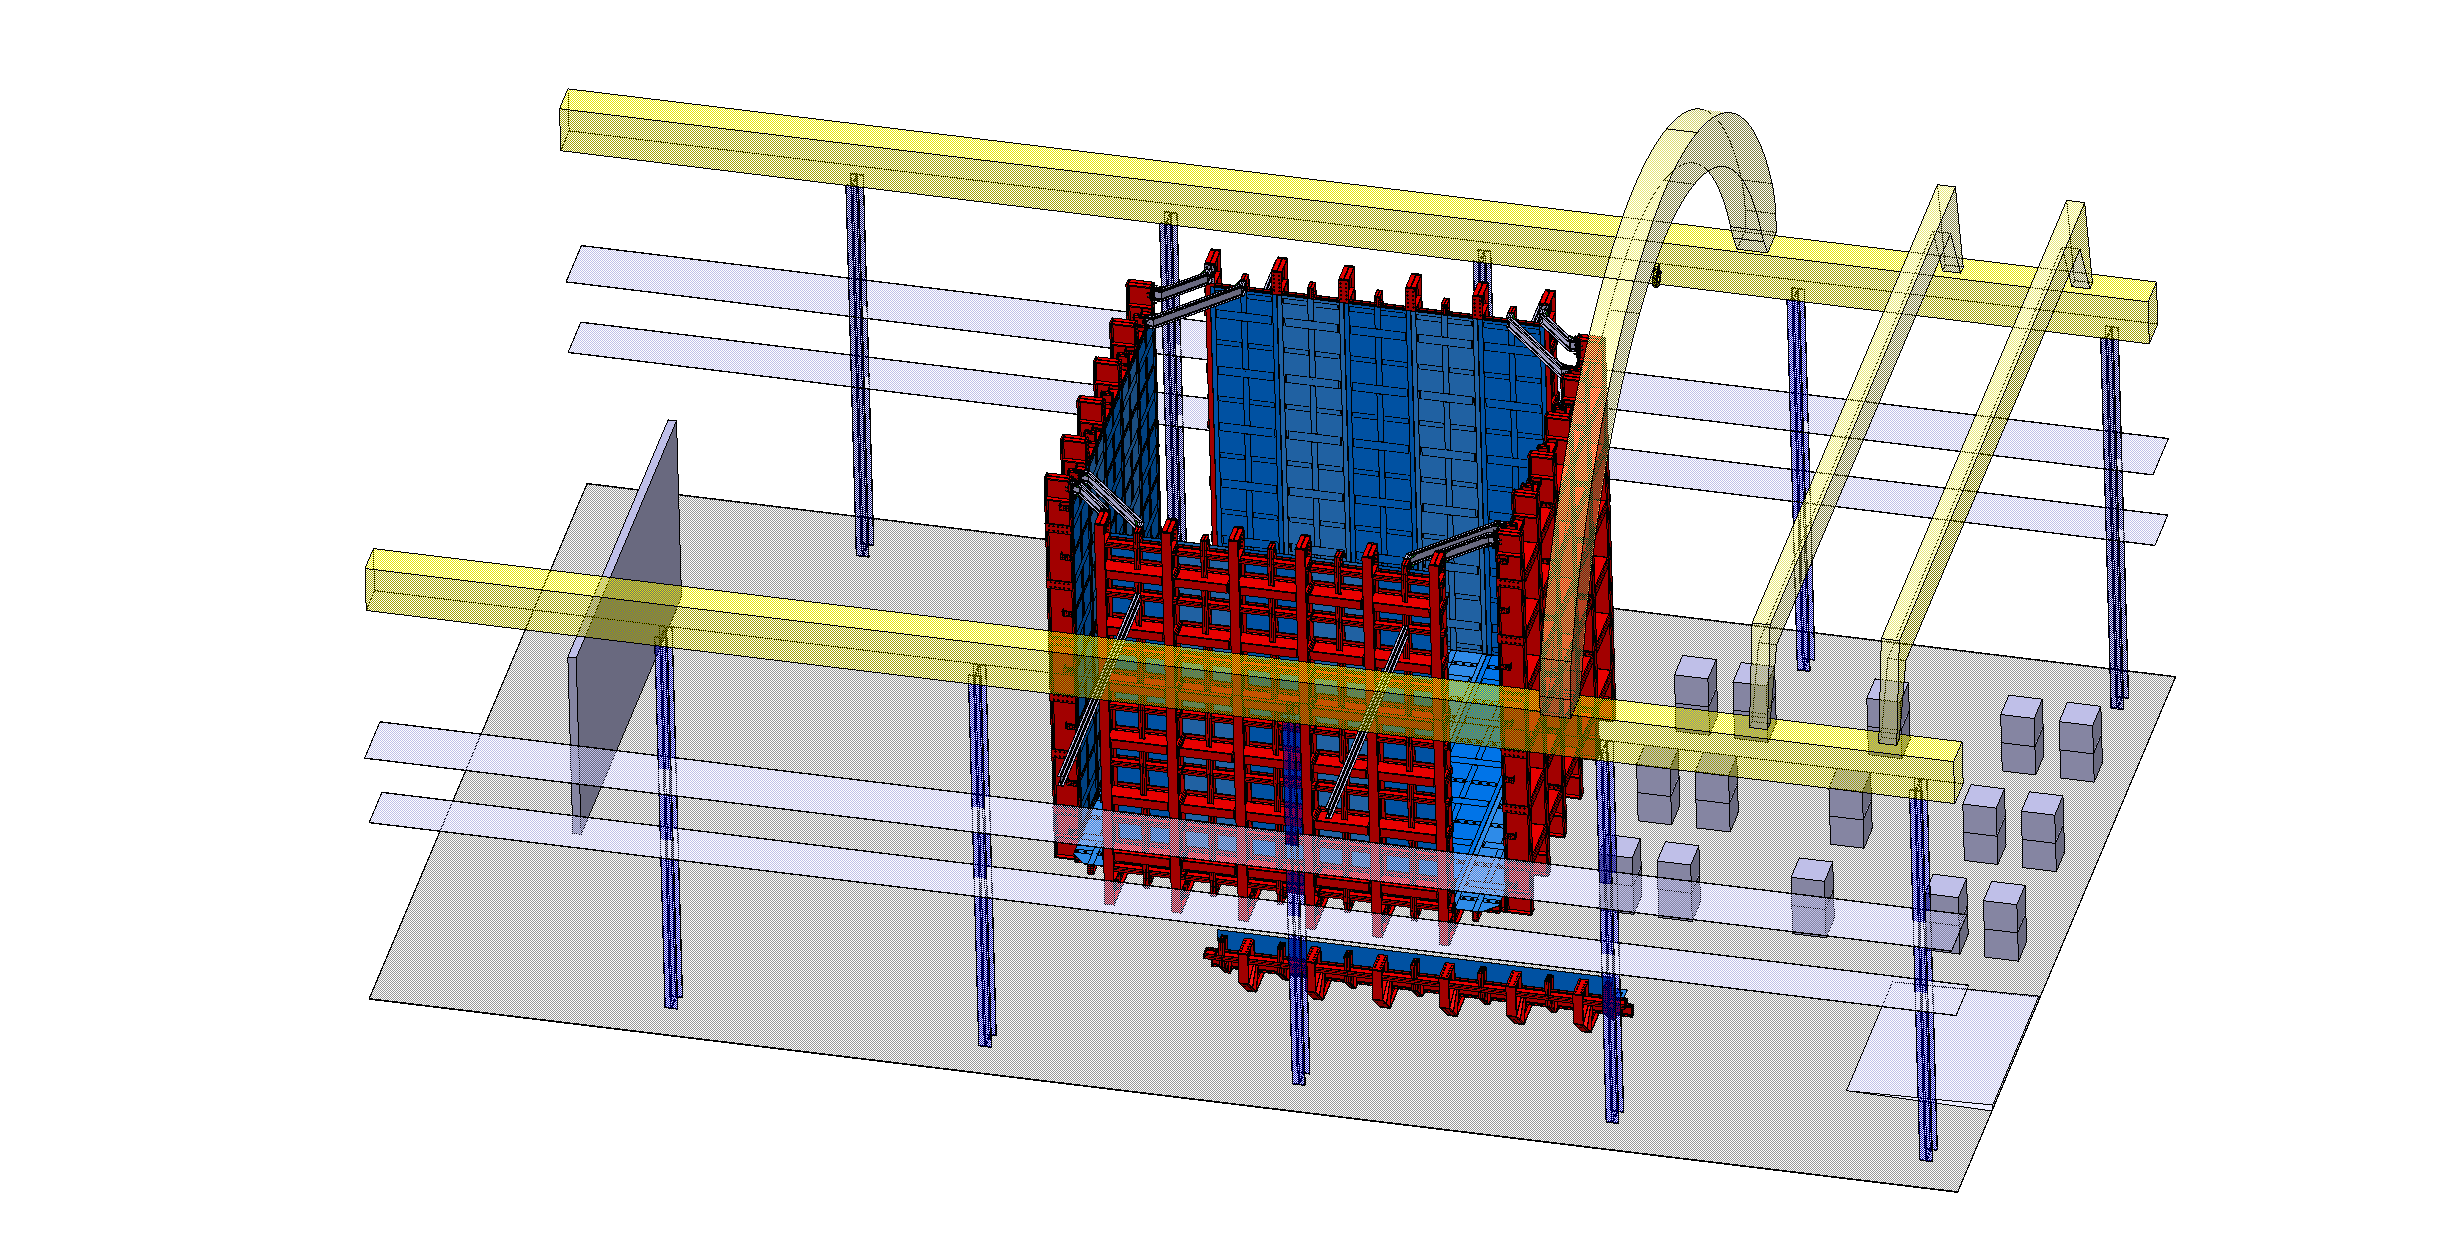
\includegraphics[width=0.32\textwidth]{./Figures/assembly_sequence_11_07/30.png}}
\subfigure[]{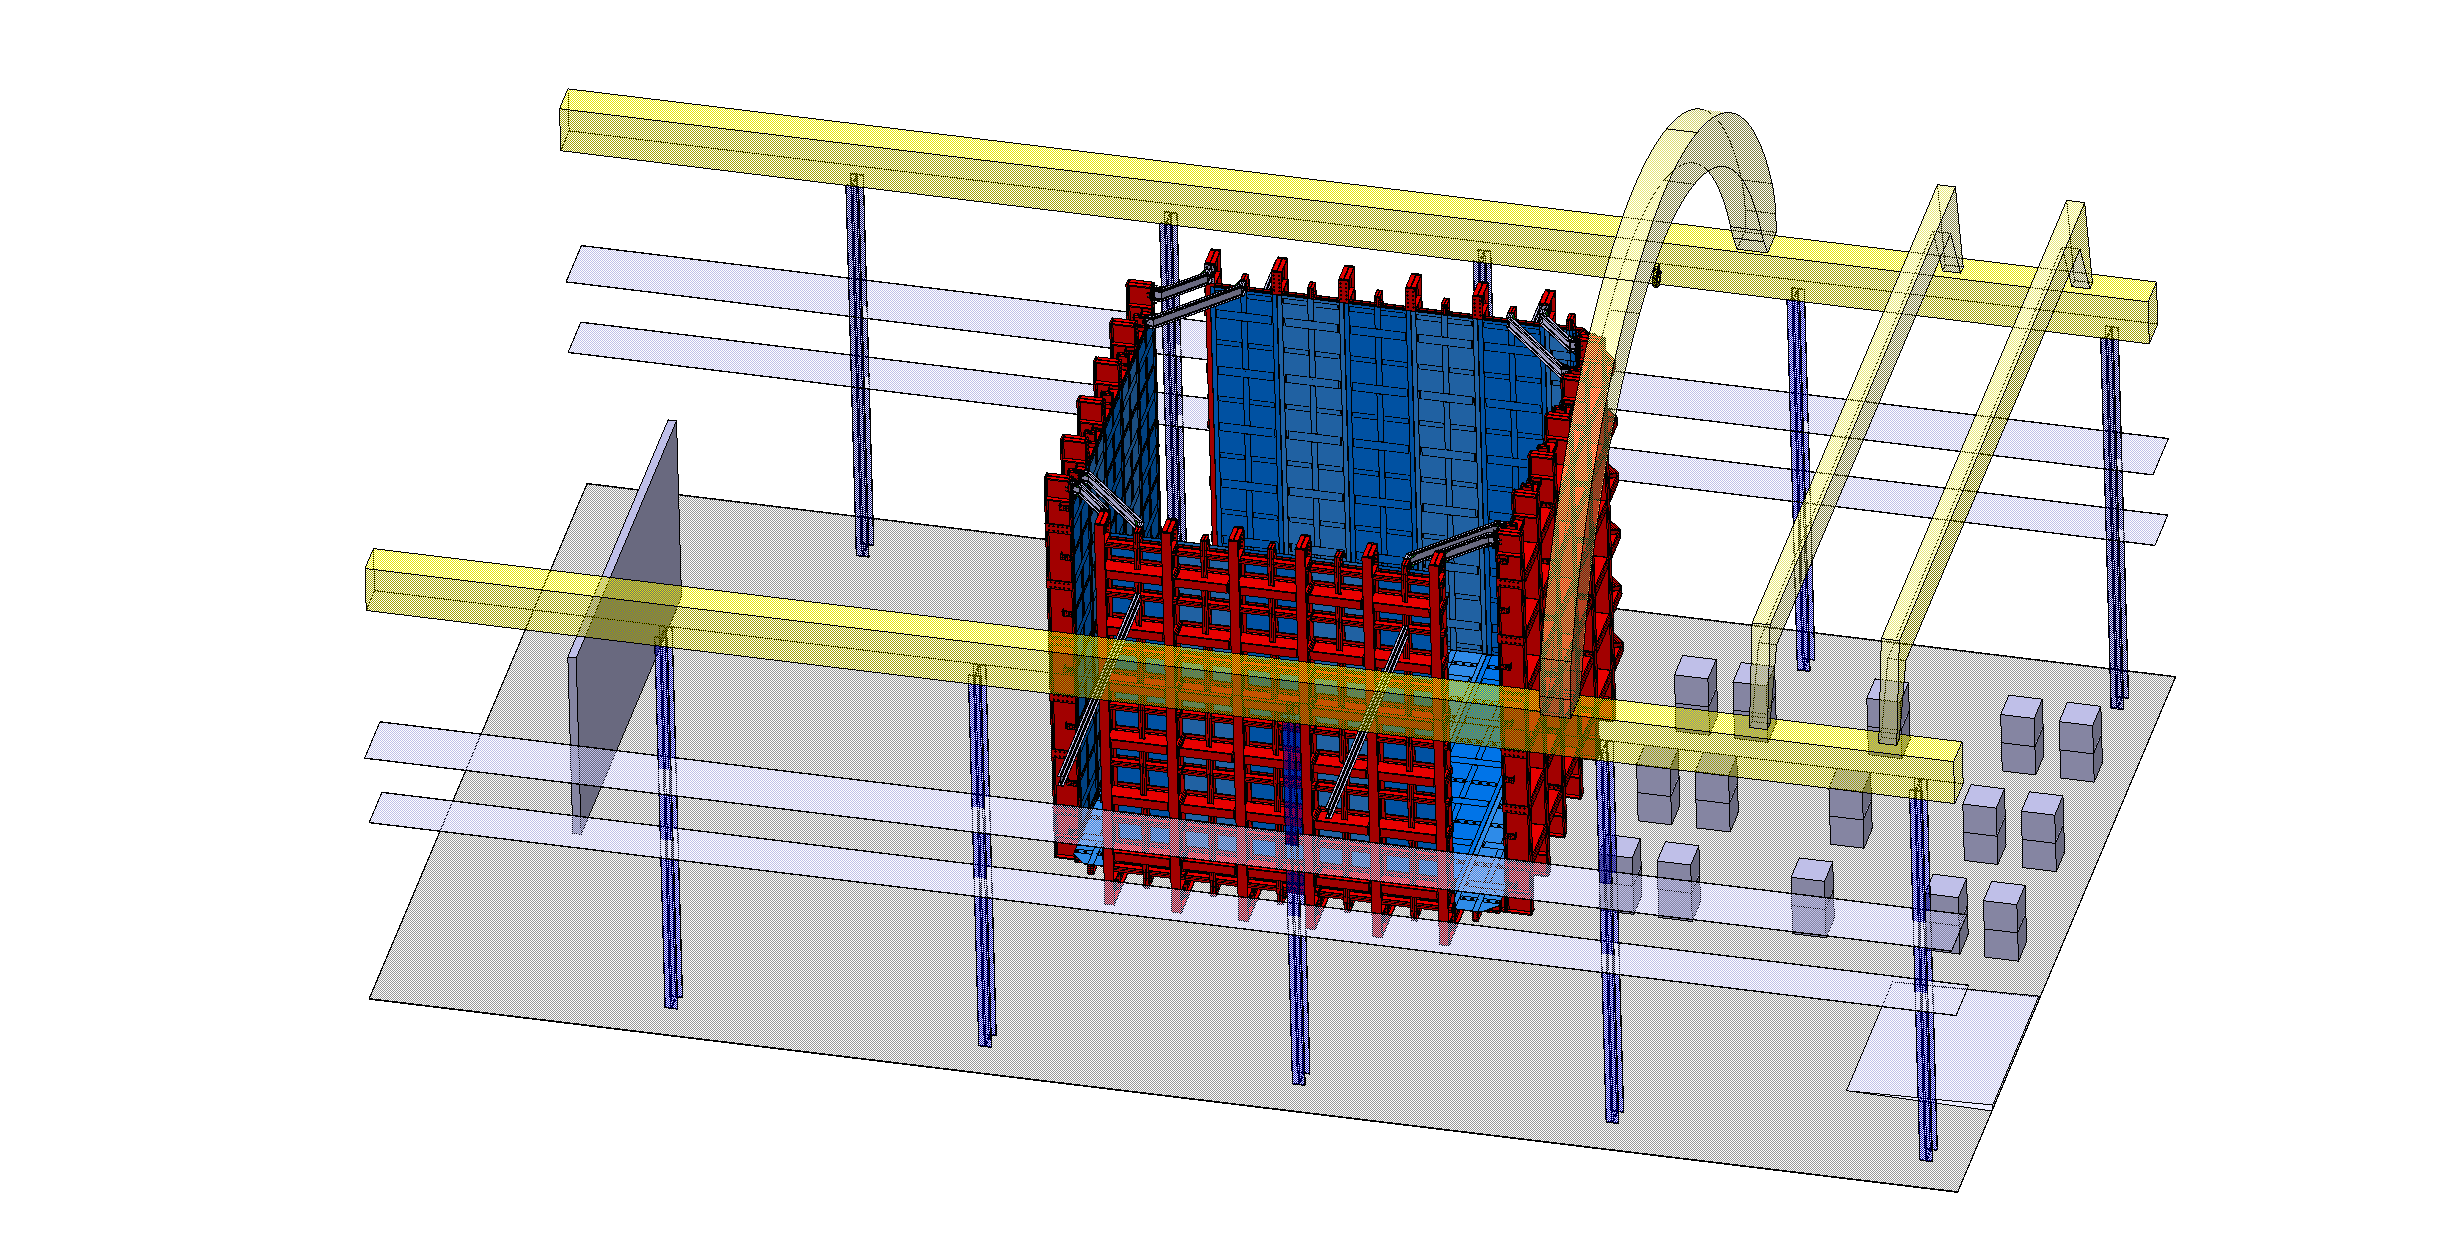
\includegraphics[width=0.32\textwidth]{./Figures/assembly_sequence_11_07/31.png}}
\subfigure[]{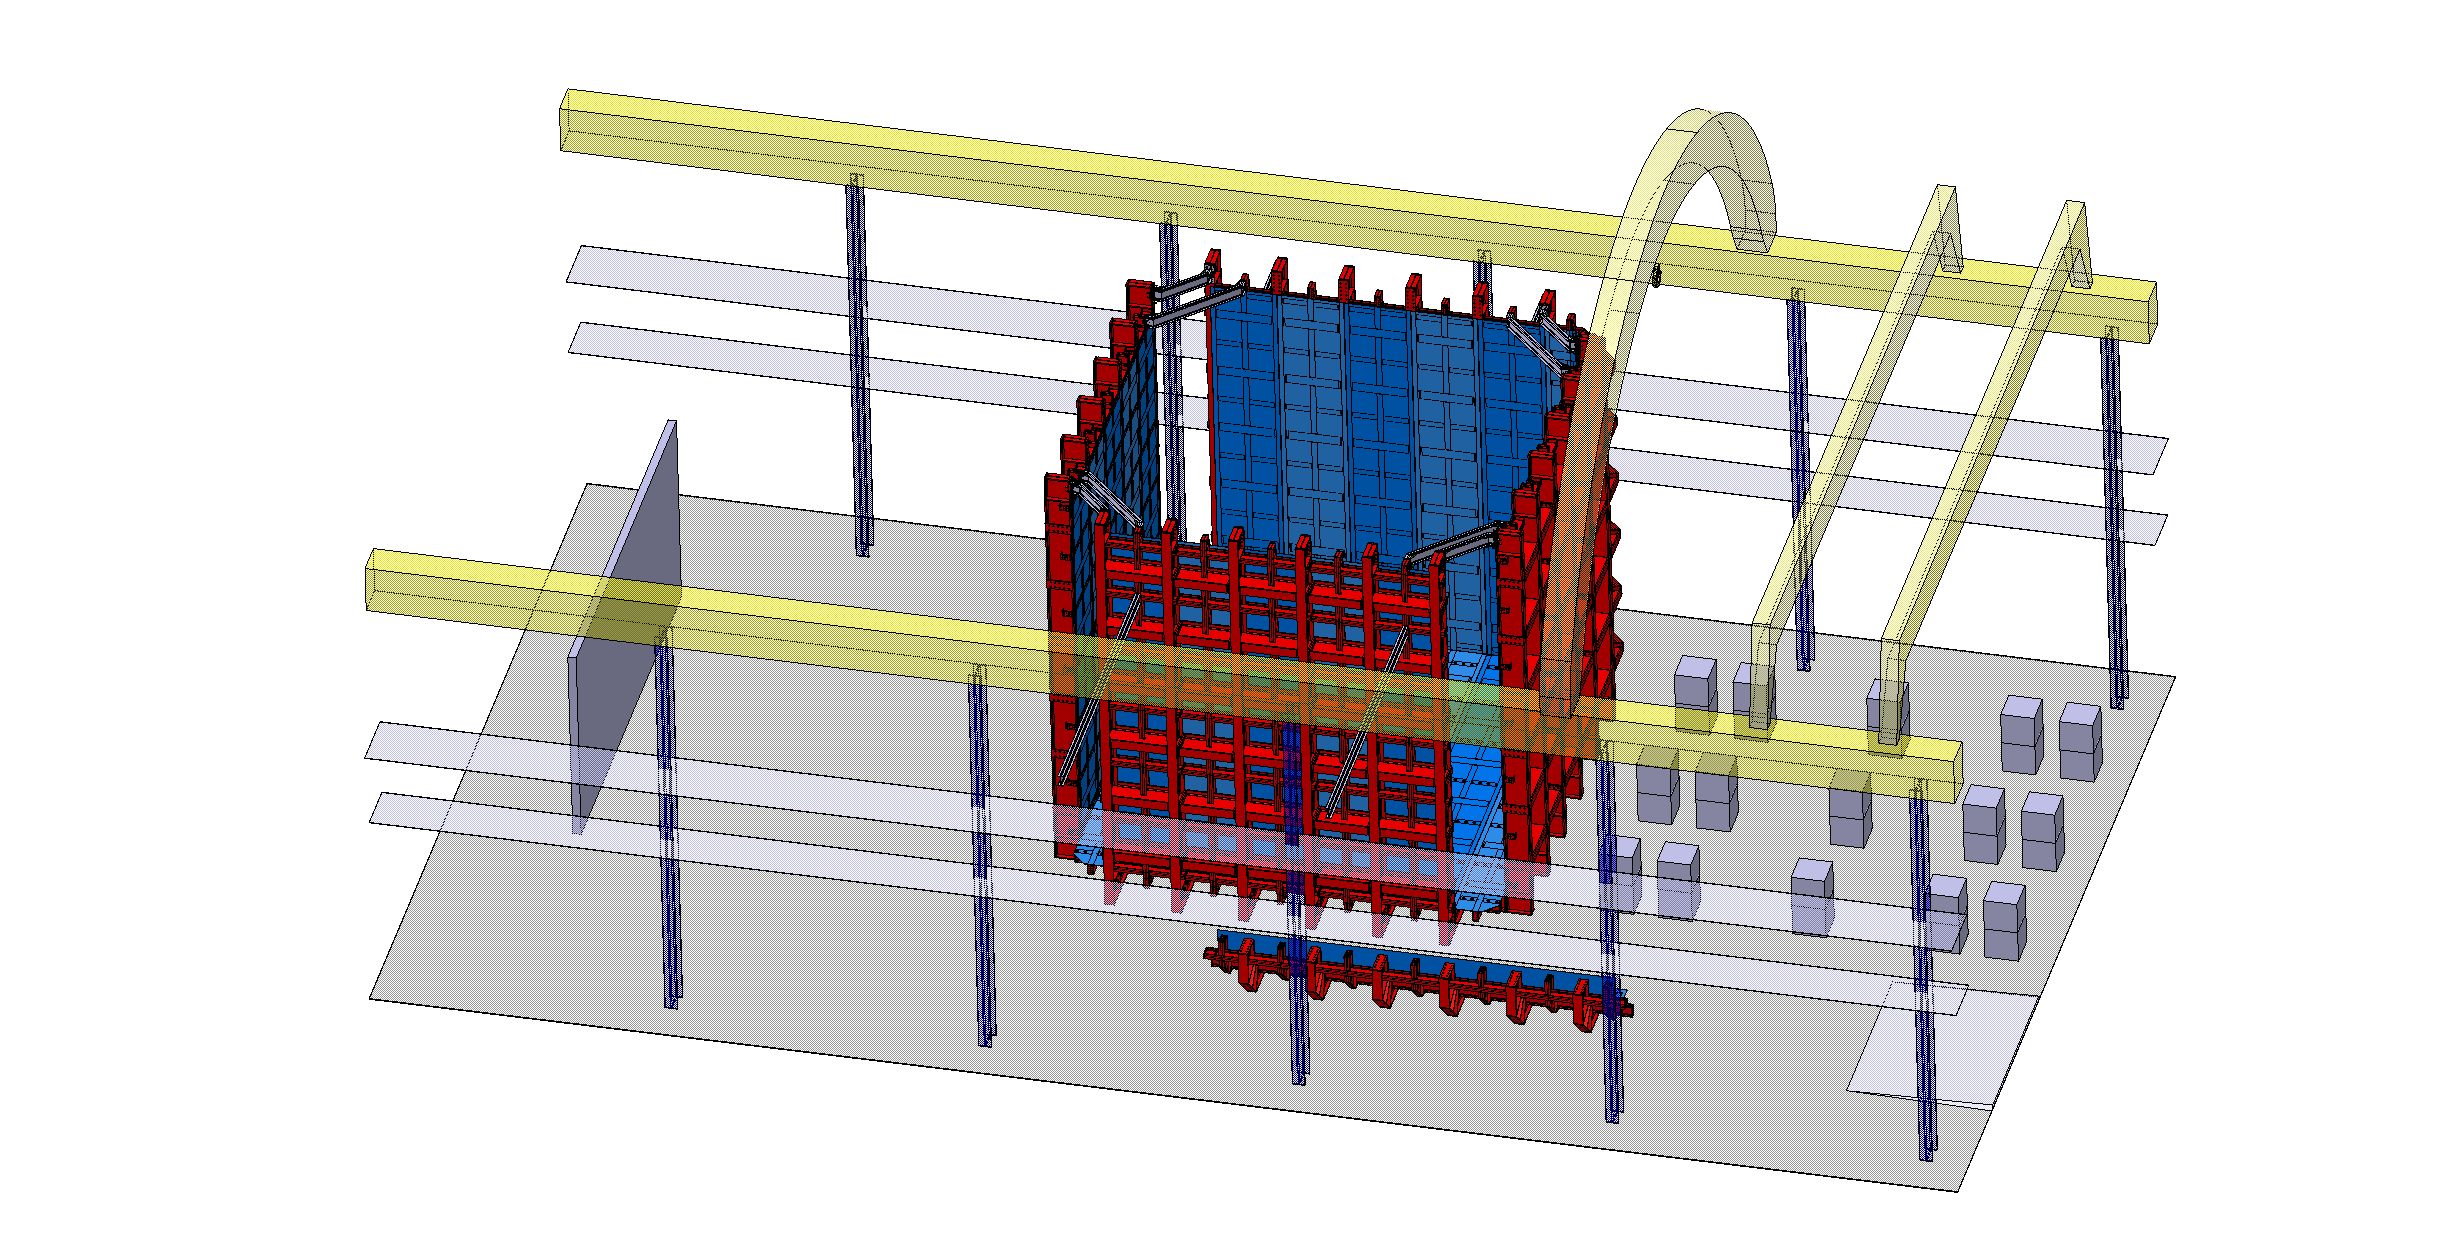
\includegraphics[width=0.32\textwidth]{./Figures/assembly_sequence_11_07/32.png}}
\subfigure[]{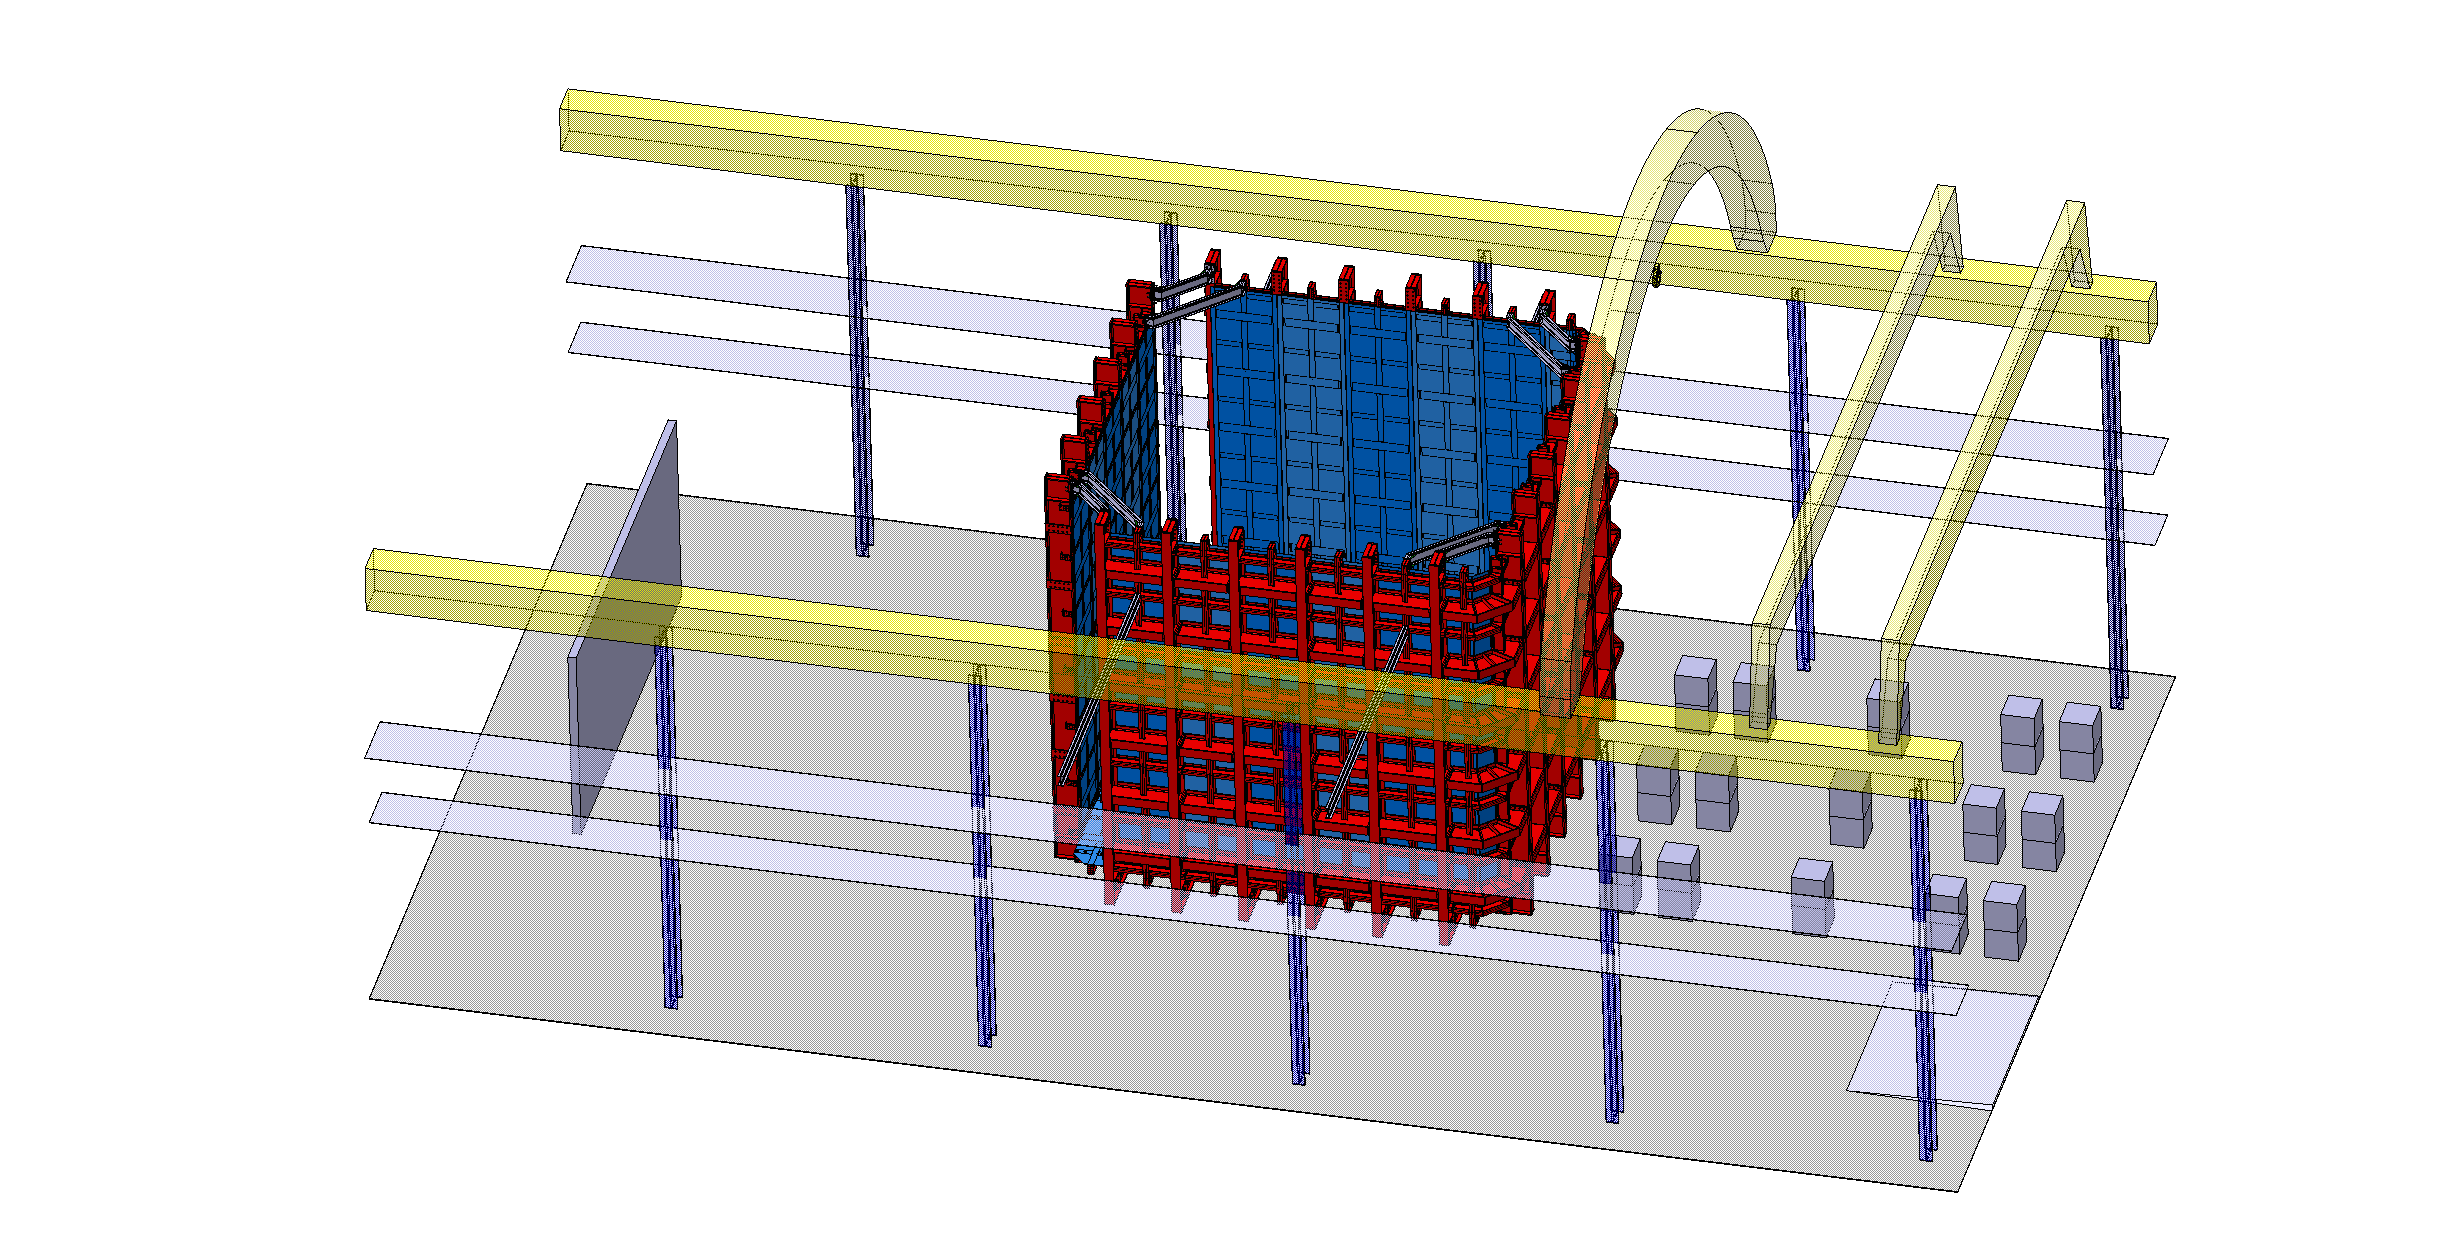
\includegraphics[width=0.32\textwidth]{./Figures/assembly_sequence_11_07/33.png}}
\subfigure[]{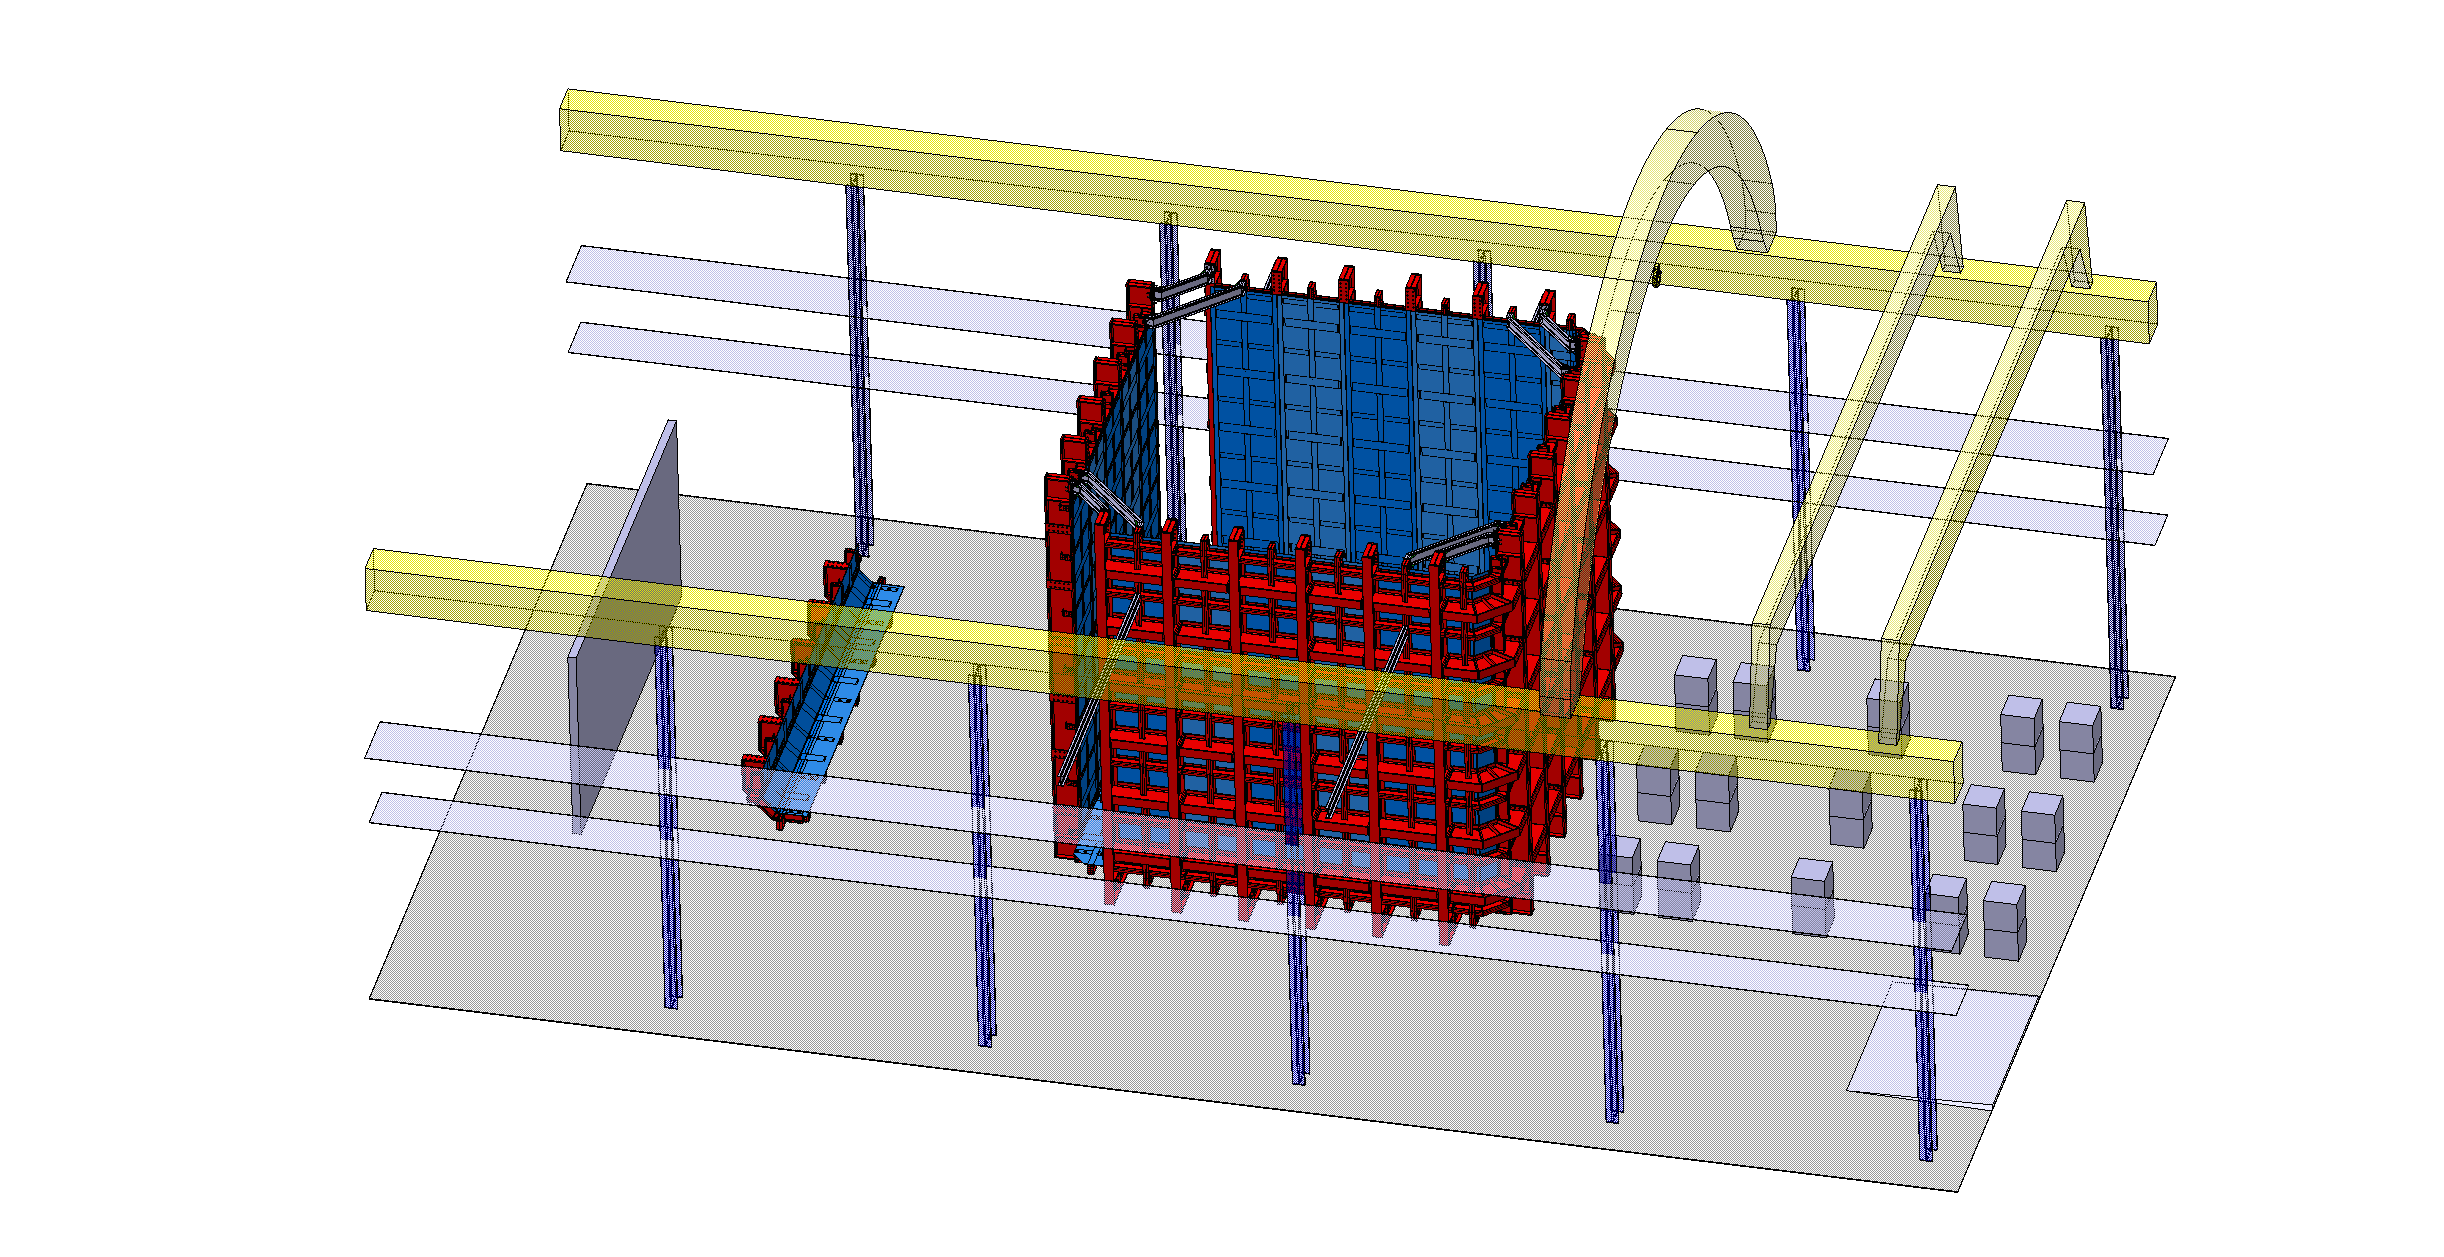
\includegraphics[width=0.32\textwidth]{./Figures/assembly_sequence_11_07/34.png}}
\subfigure[]{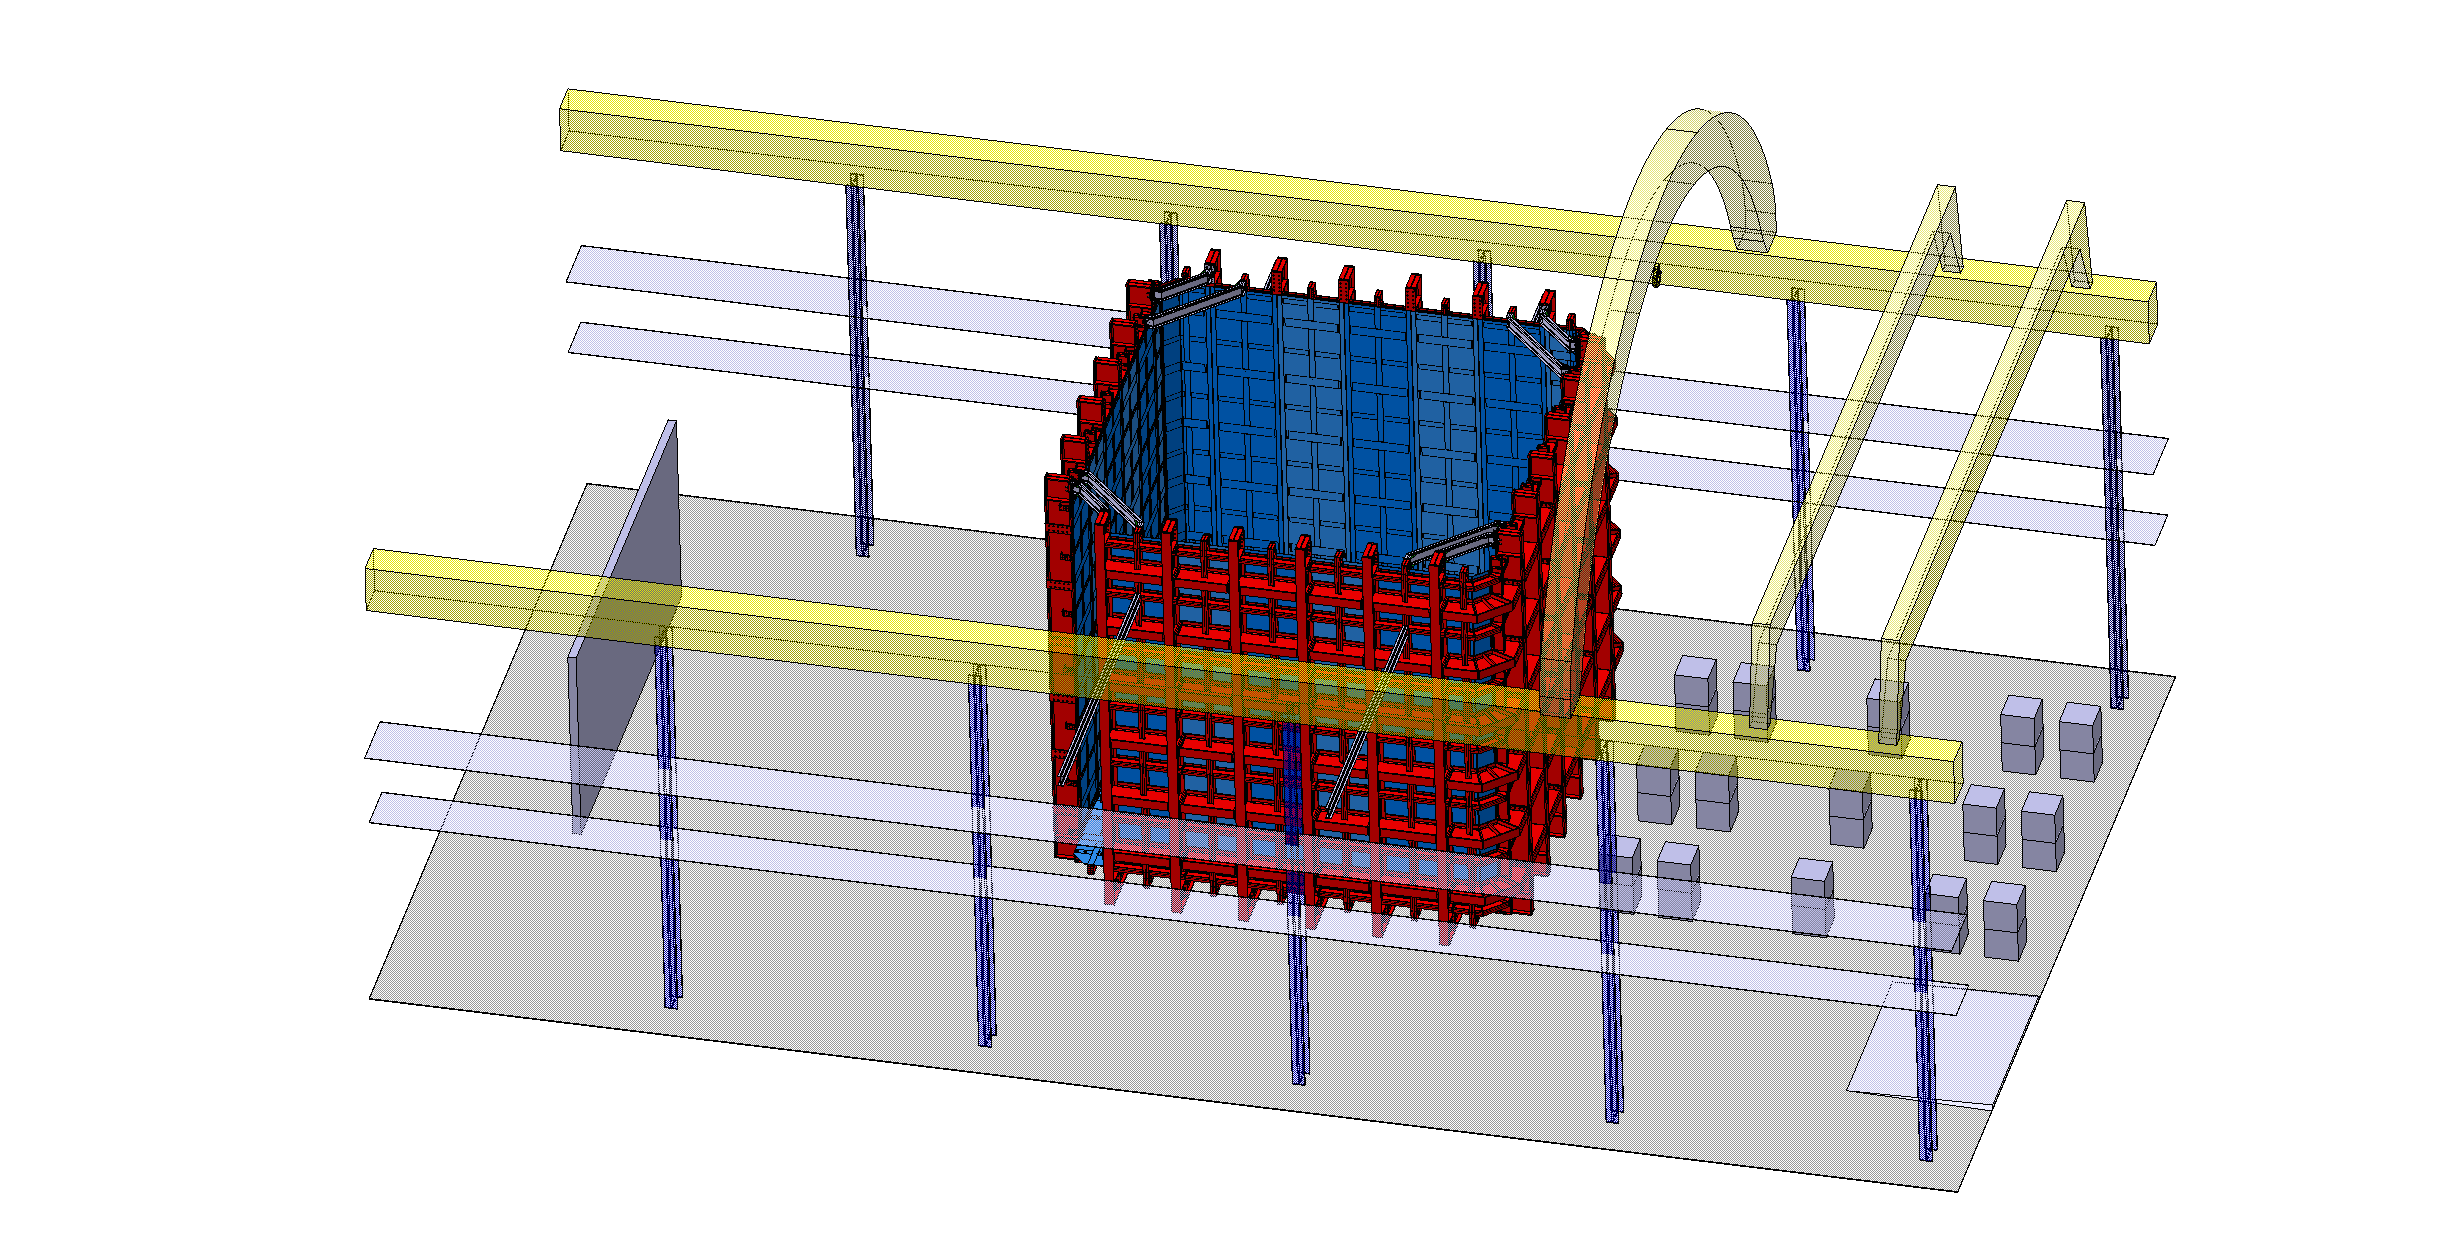
\includegraphics[width=0.32\textwidth]{./Figures/assembly_sequence_11_07/35.png}}
\caption{Details of the installation sequence (II) }
\label{fig:Ds20kInstallSequence2}
\end{figure*}

\begin{figure*}[!t]
\subfigure[]{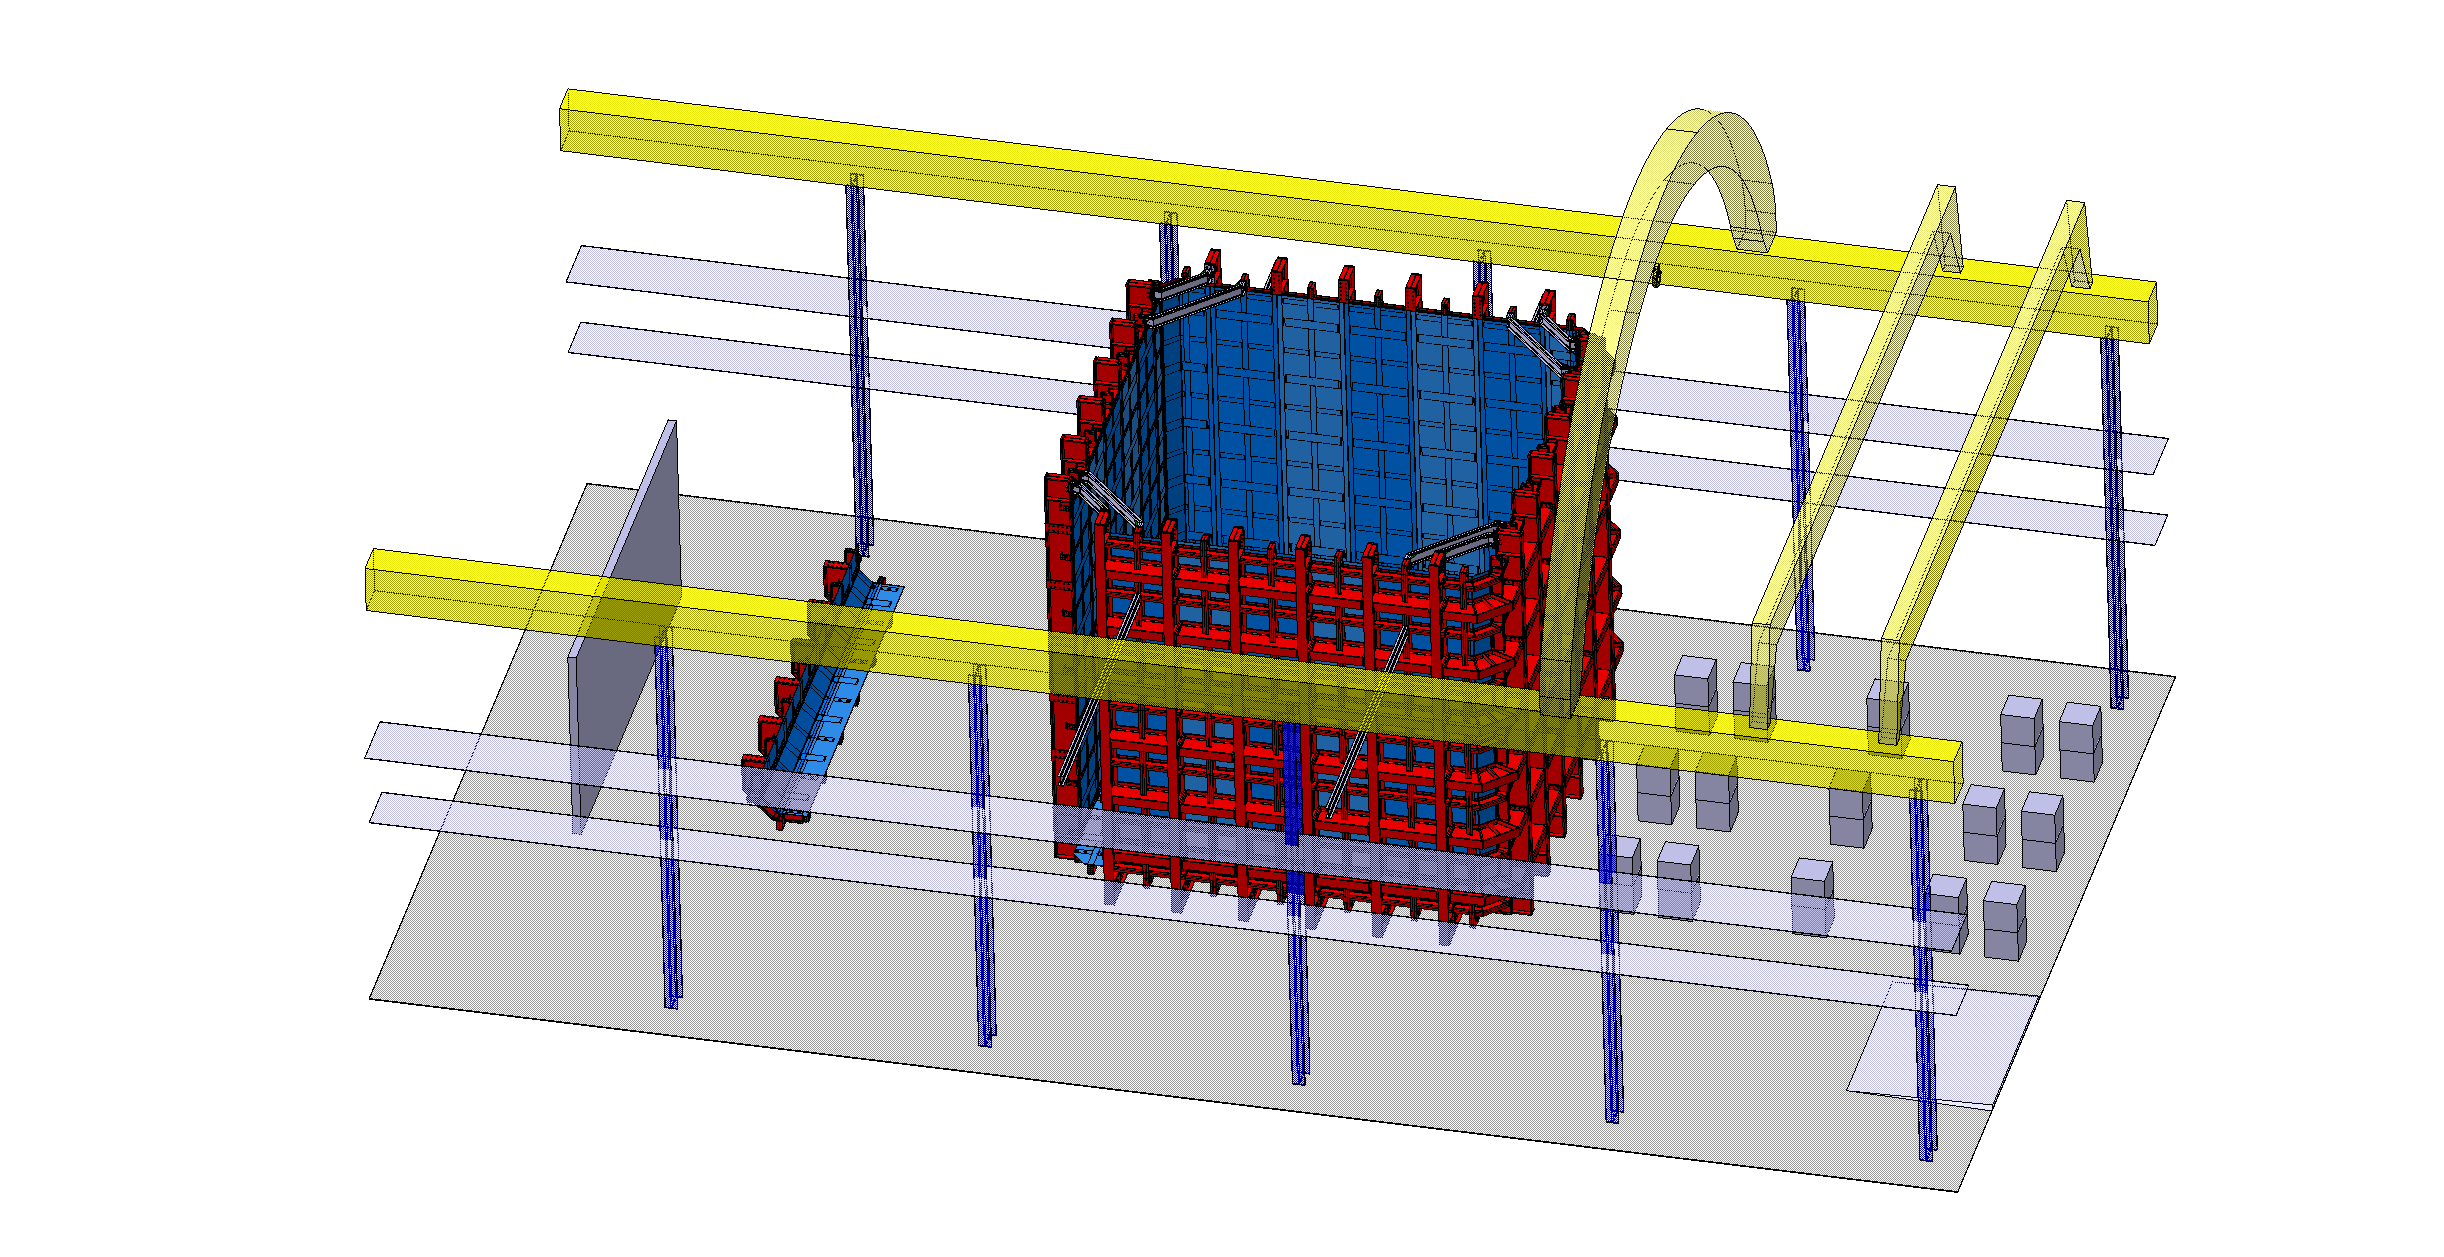
\includegraphics[width=0.32\textwidth]{./Figures/assembly_sequence_11_07/36.png}}
\subfigure[]{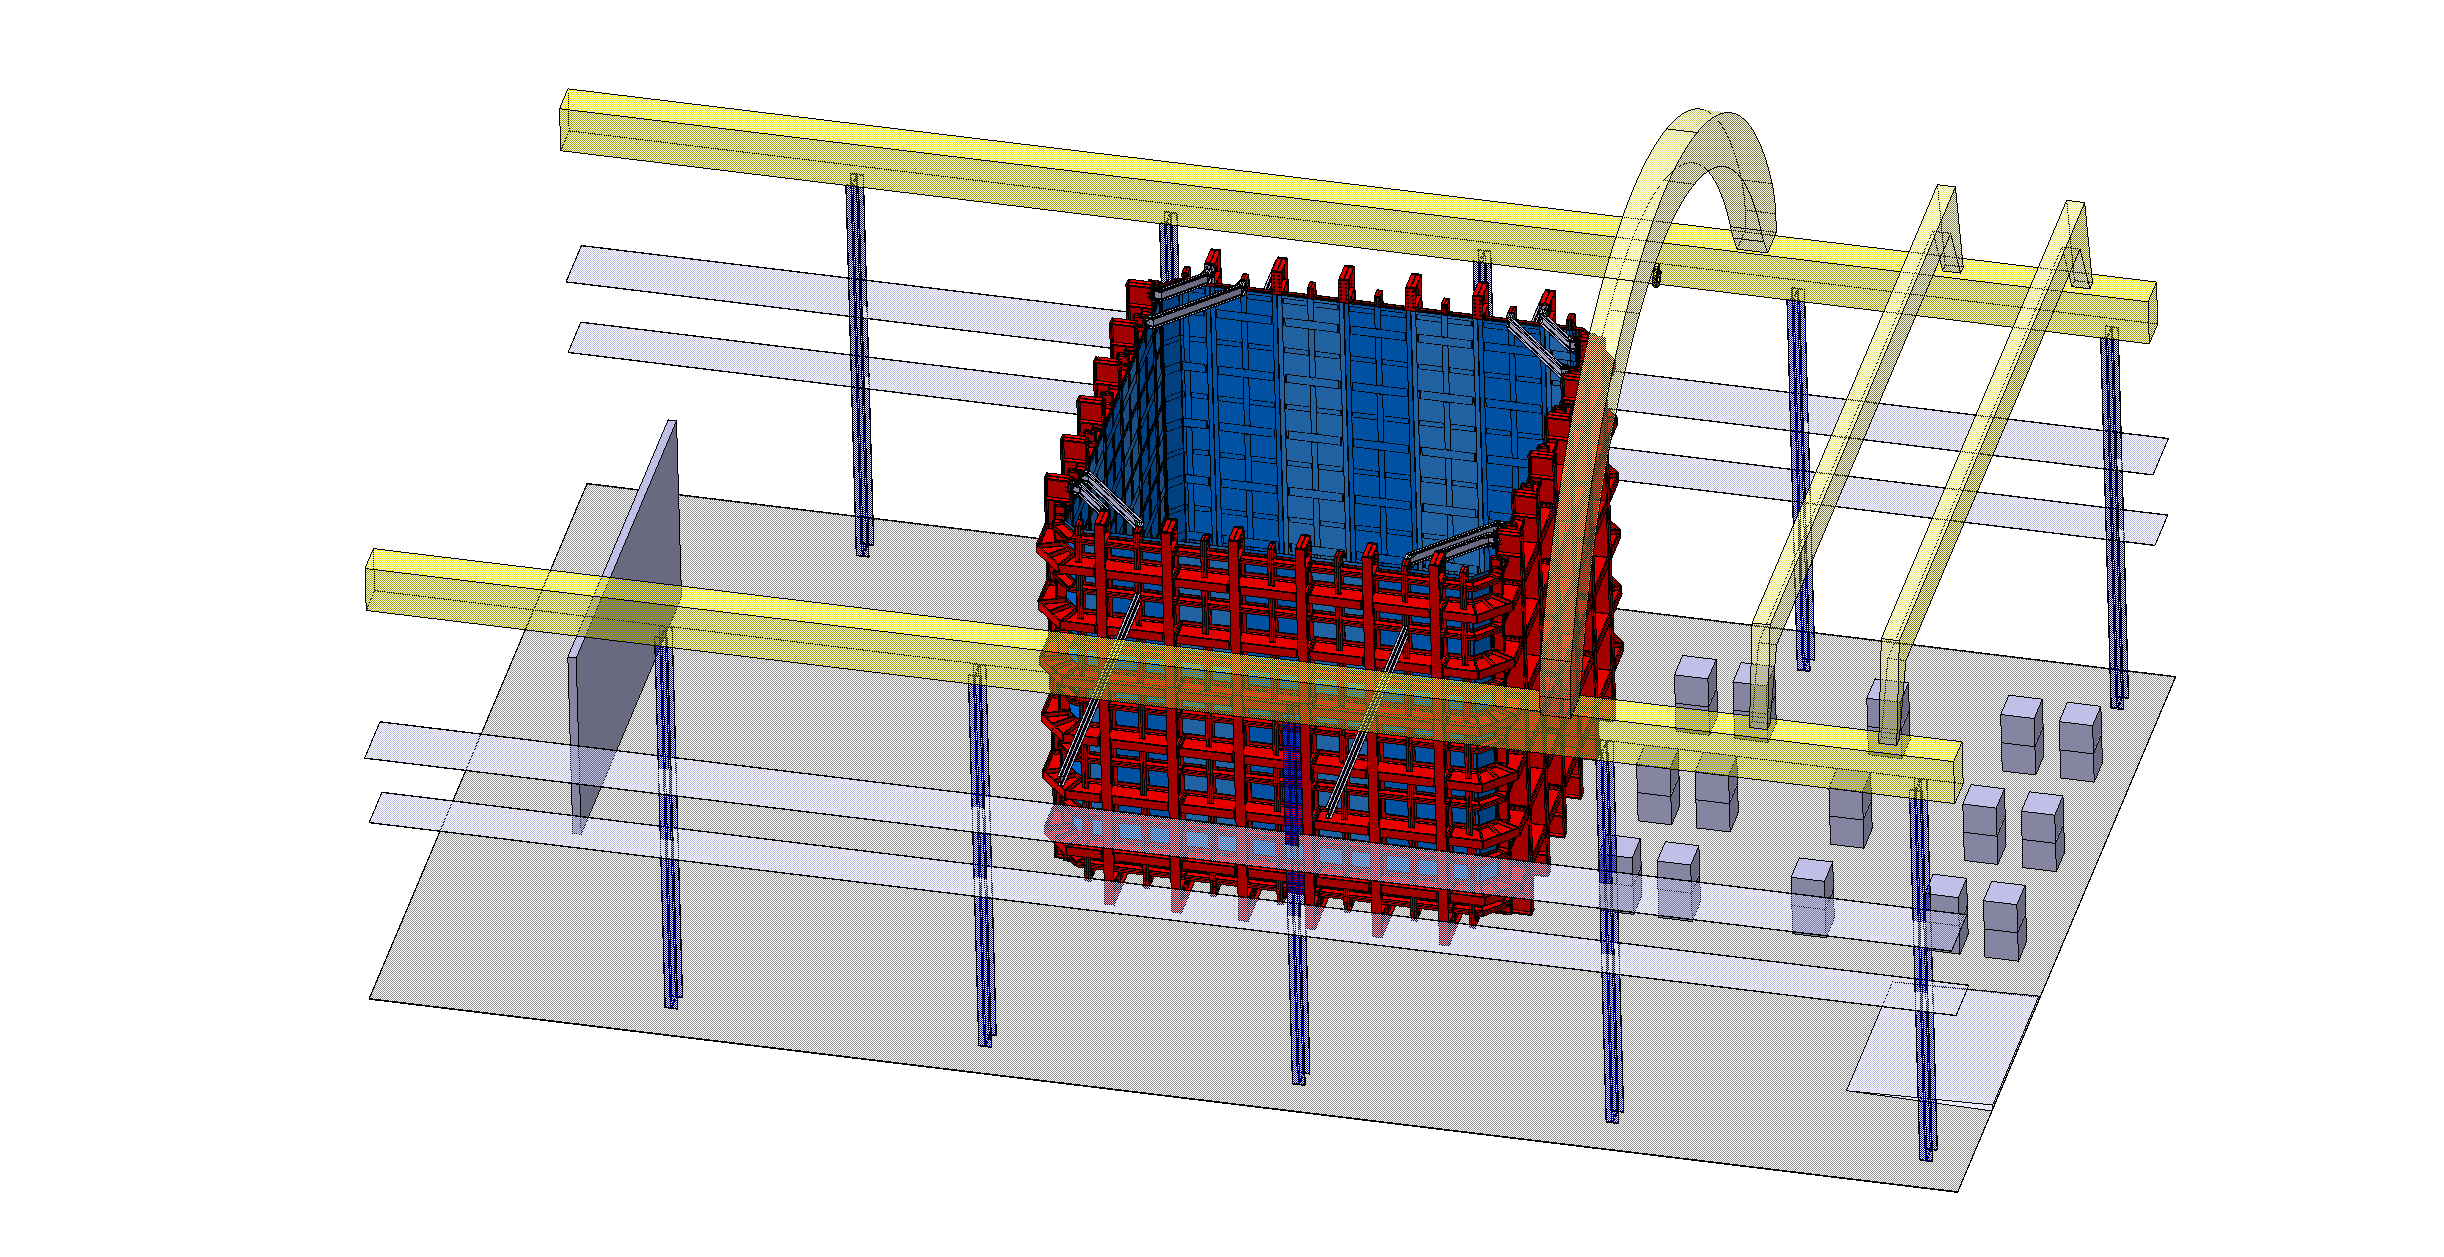
\includegraphics[width=0.32\textwidth]{./Figures/assembly_sequence_11_07/37.png}}
\subfigure[]{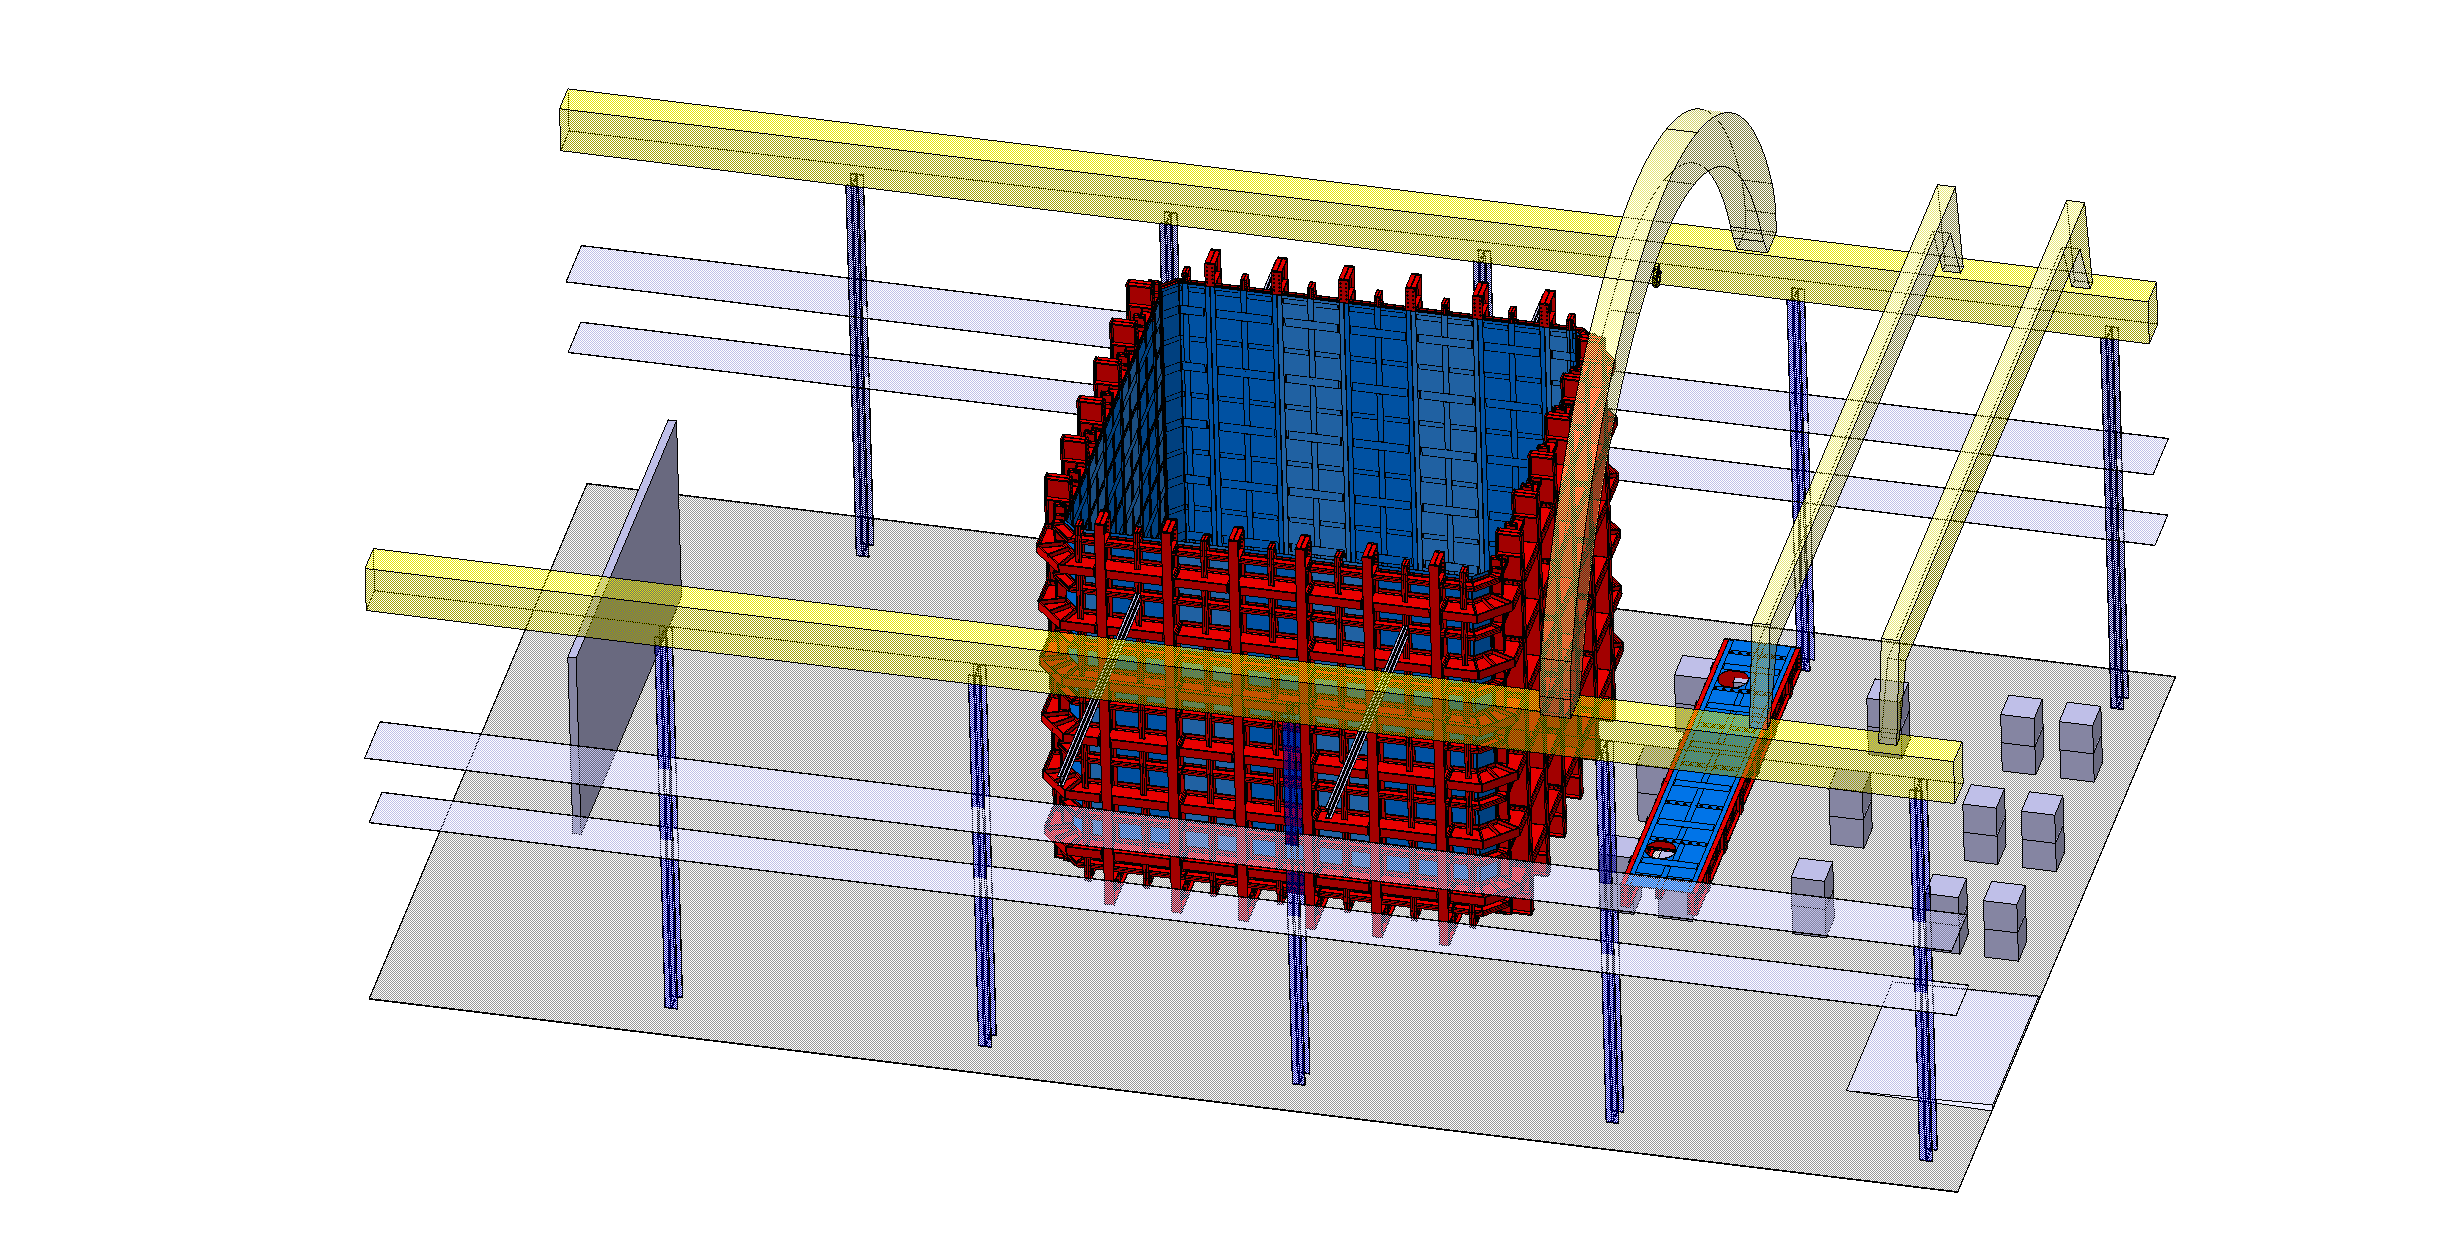
\includegraphics[width=0.32\textwidth]{./Figures/assembly_sequence_11_07/38.png}}
\subfigure[]{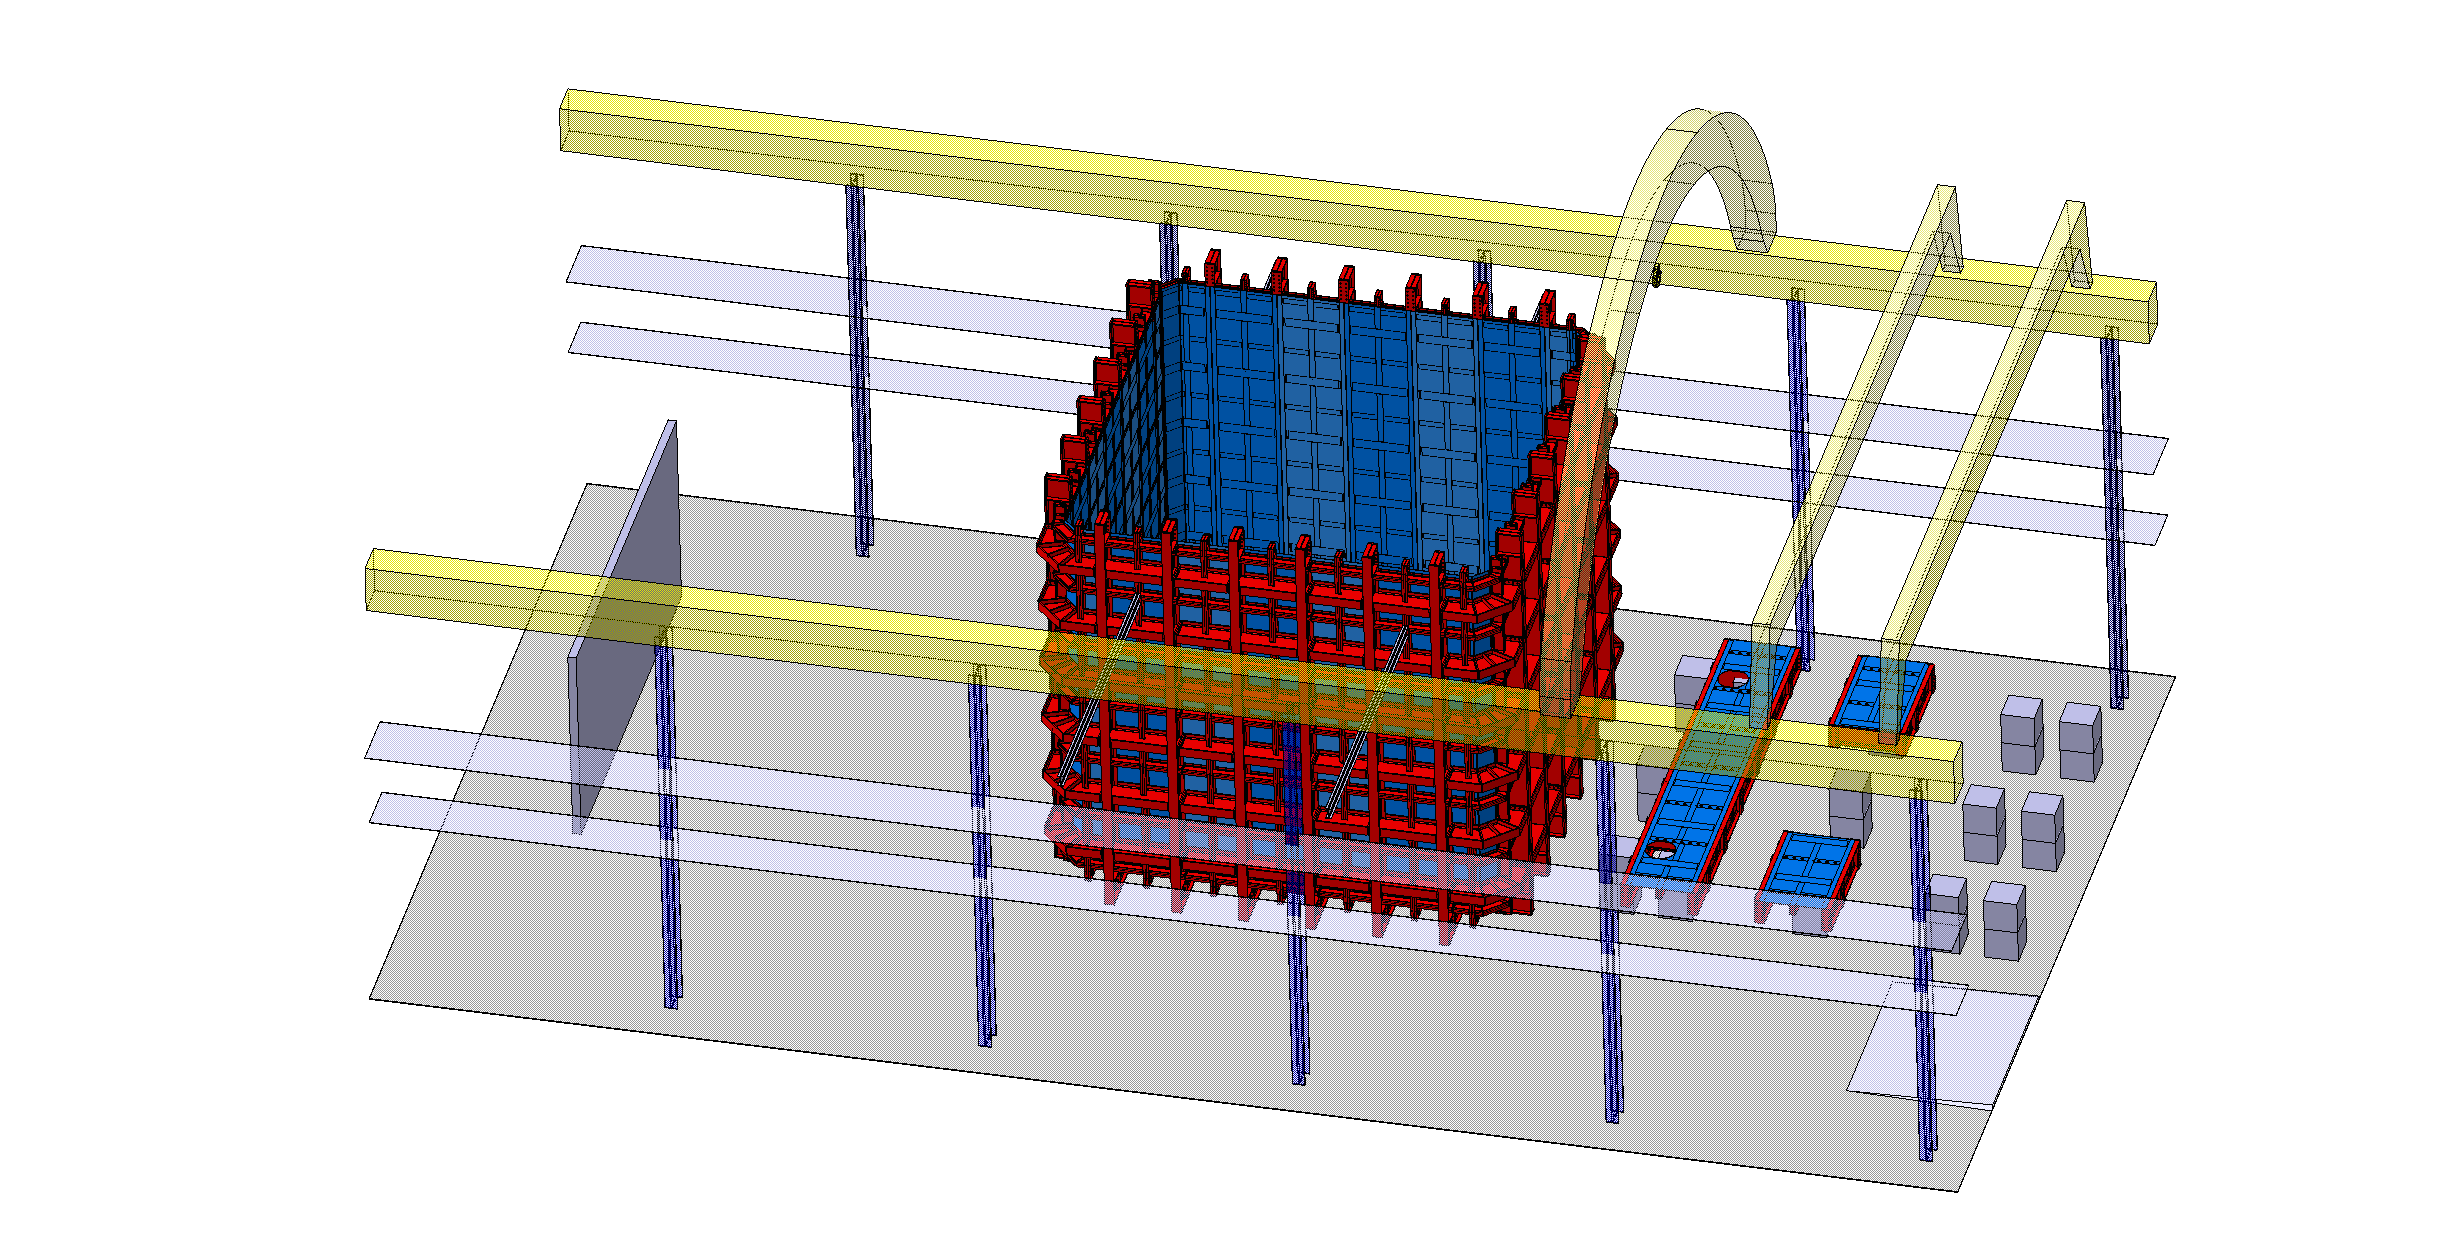
\includegraphics[width=0.32\textwidth]{./Figures/assembly_sequence_11_07/39.png}}
\subfigure[]{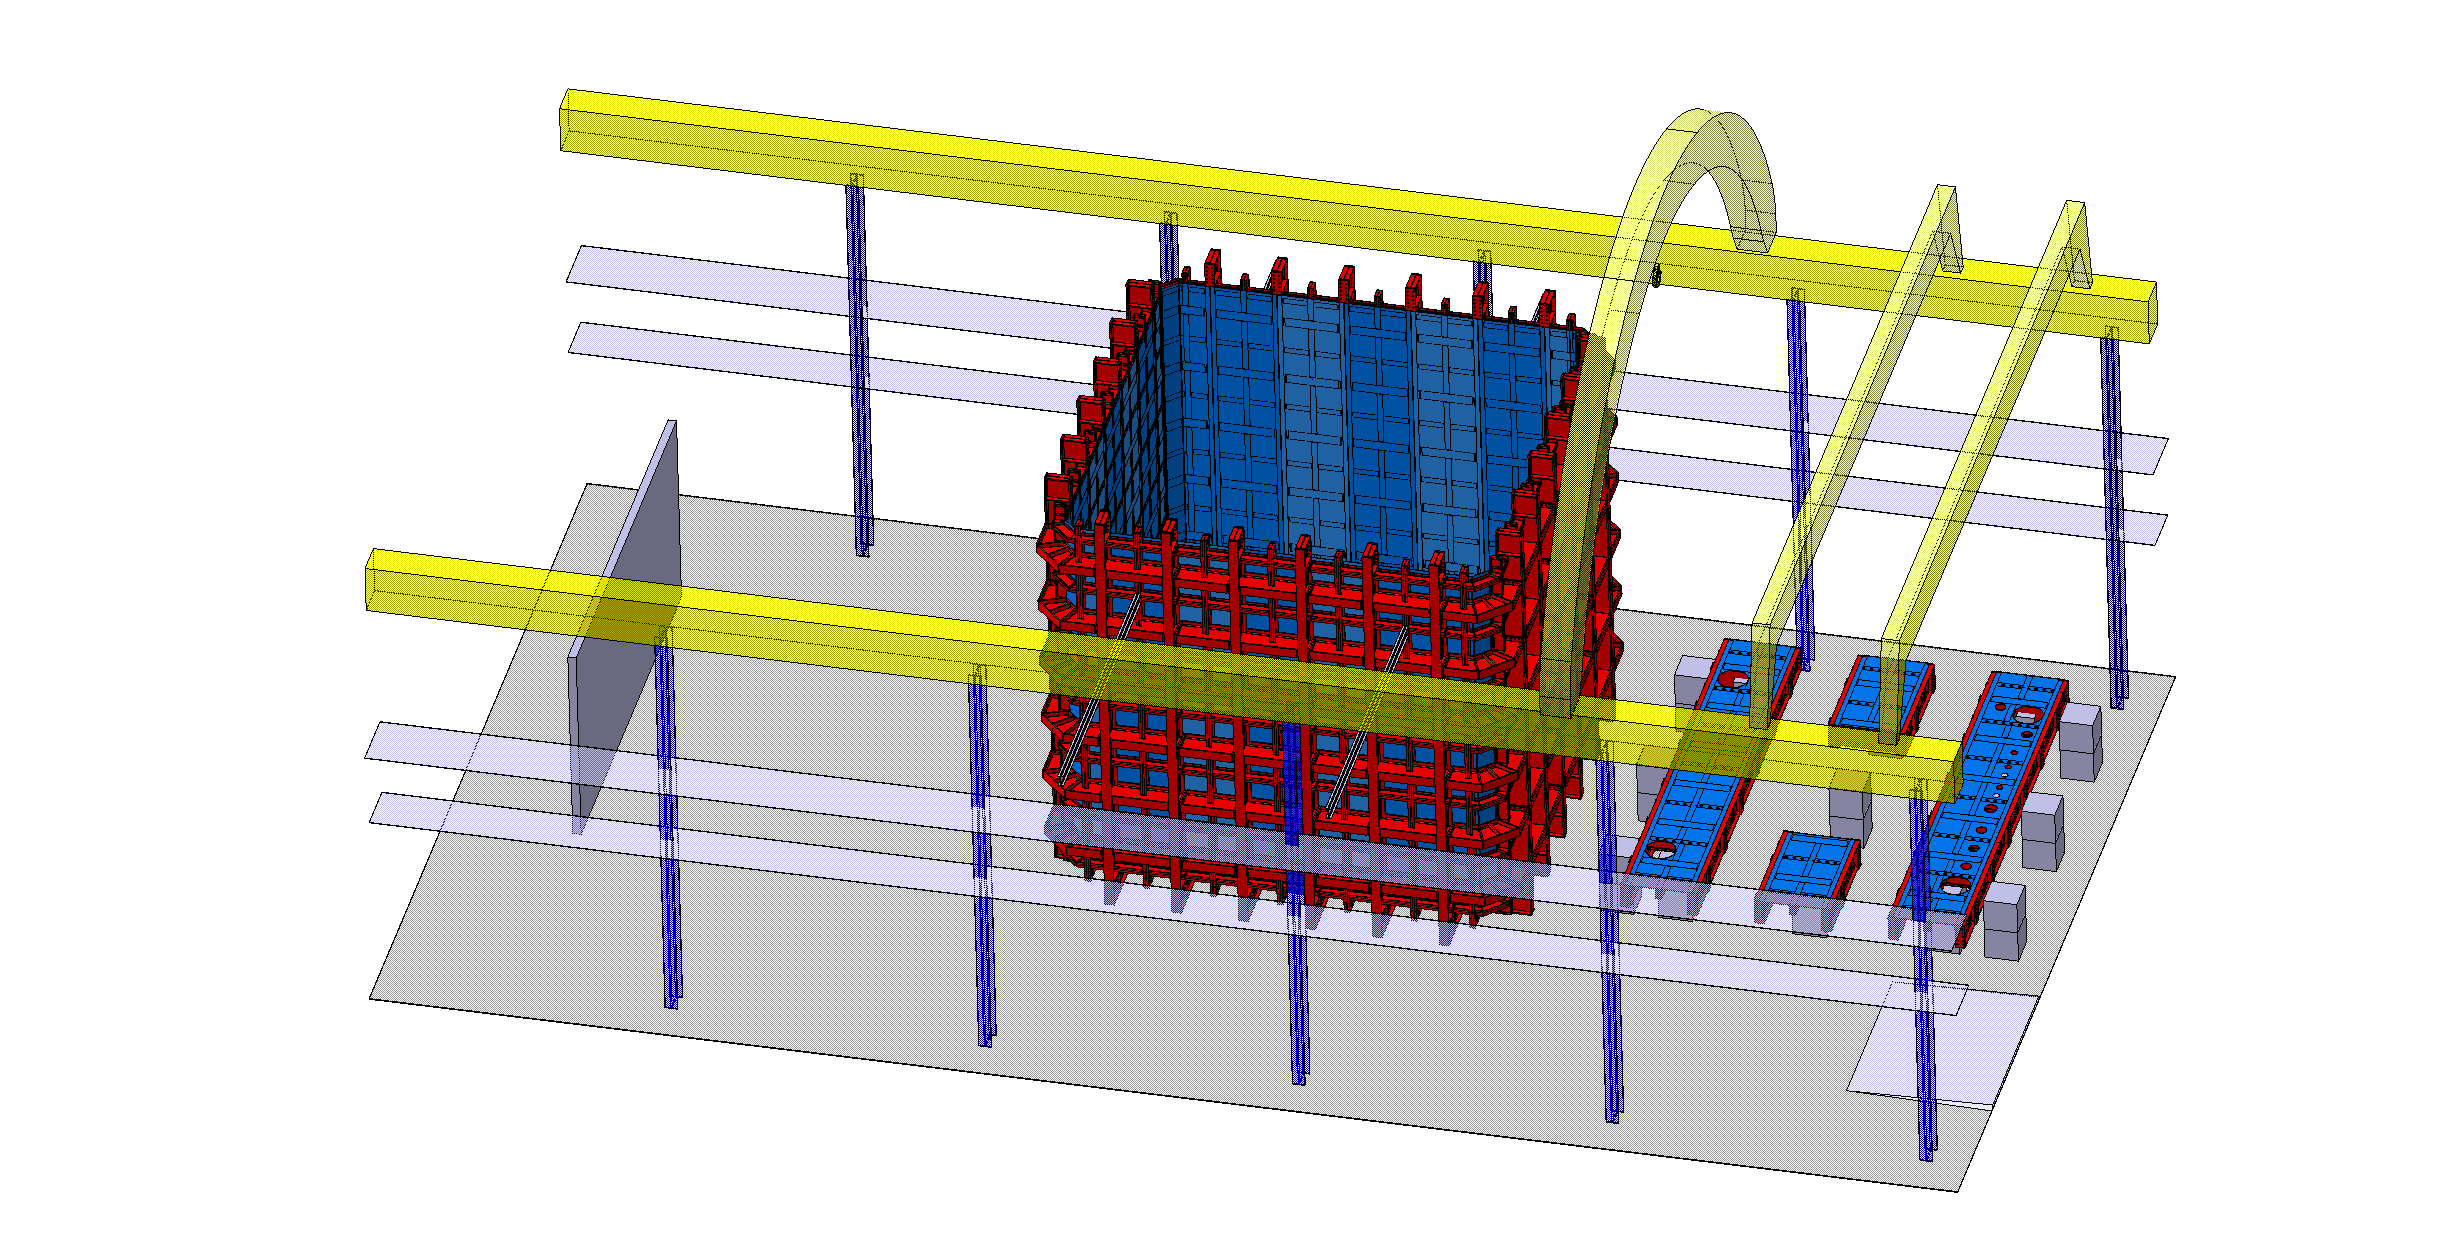
\includegraphics[width=0.32\textwidth]{./Figures/assembly_sequence_11_07/40.png}}
\subfigure[]{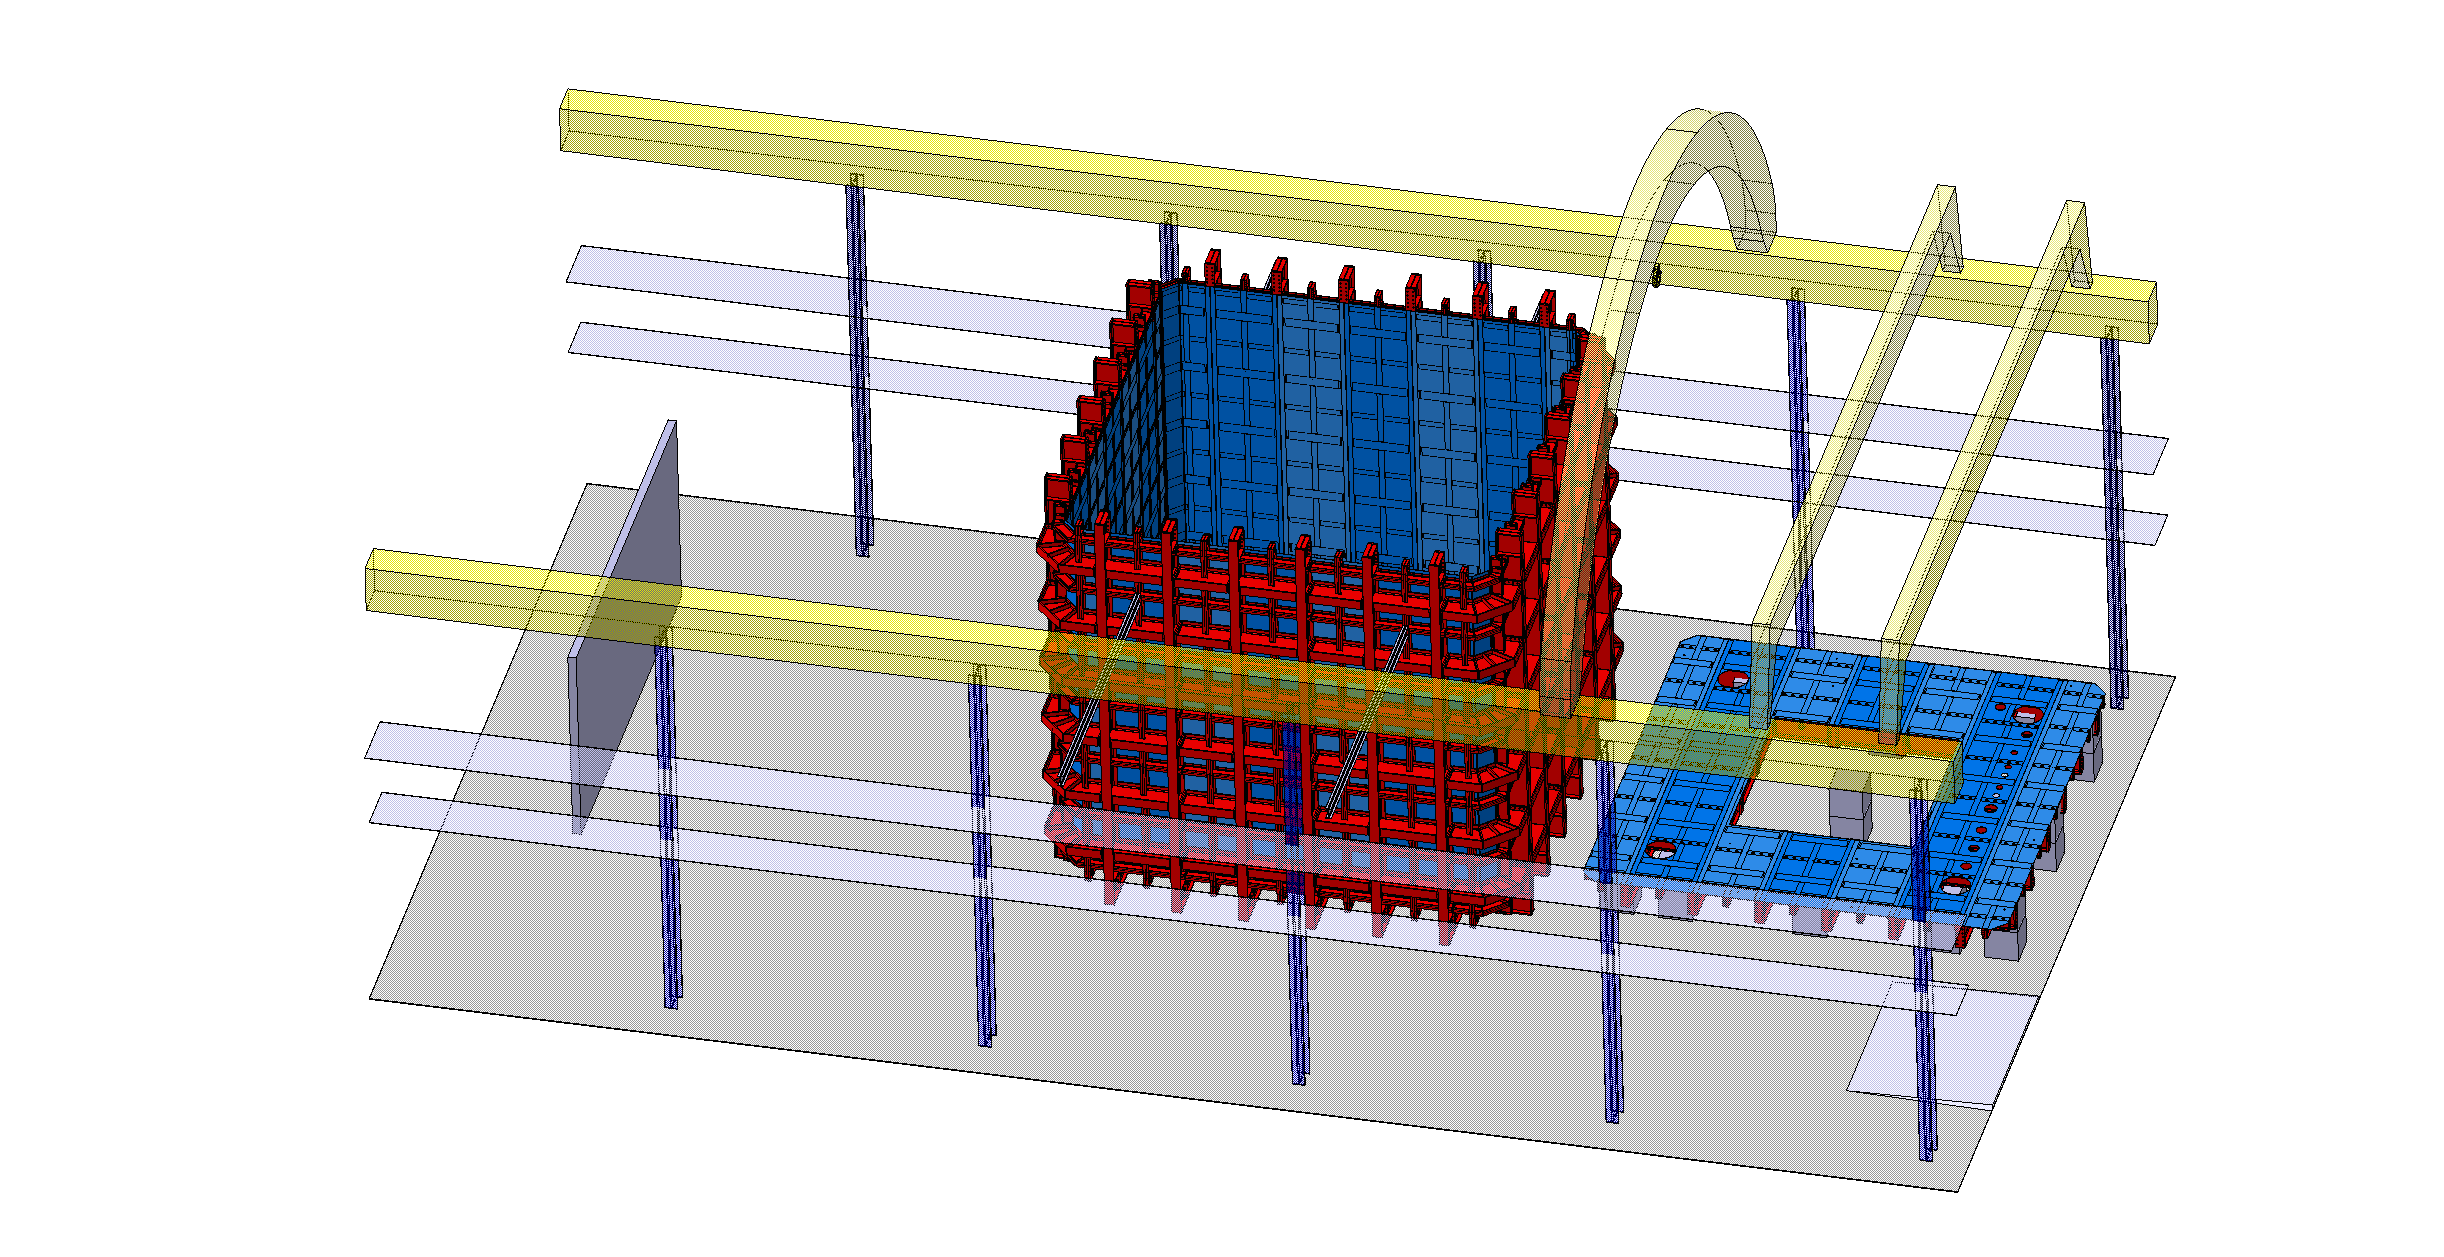
\includegraphics[width=0.32\textwidth]{./Figures/assembly_sequence_11_07/41.png}}
\subfigure[]{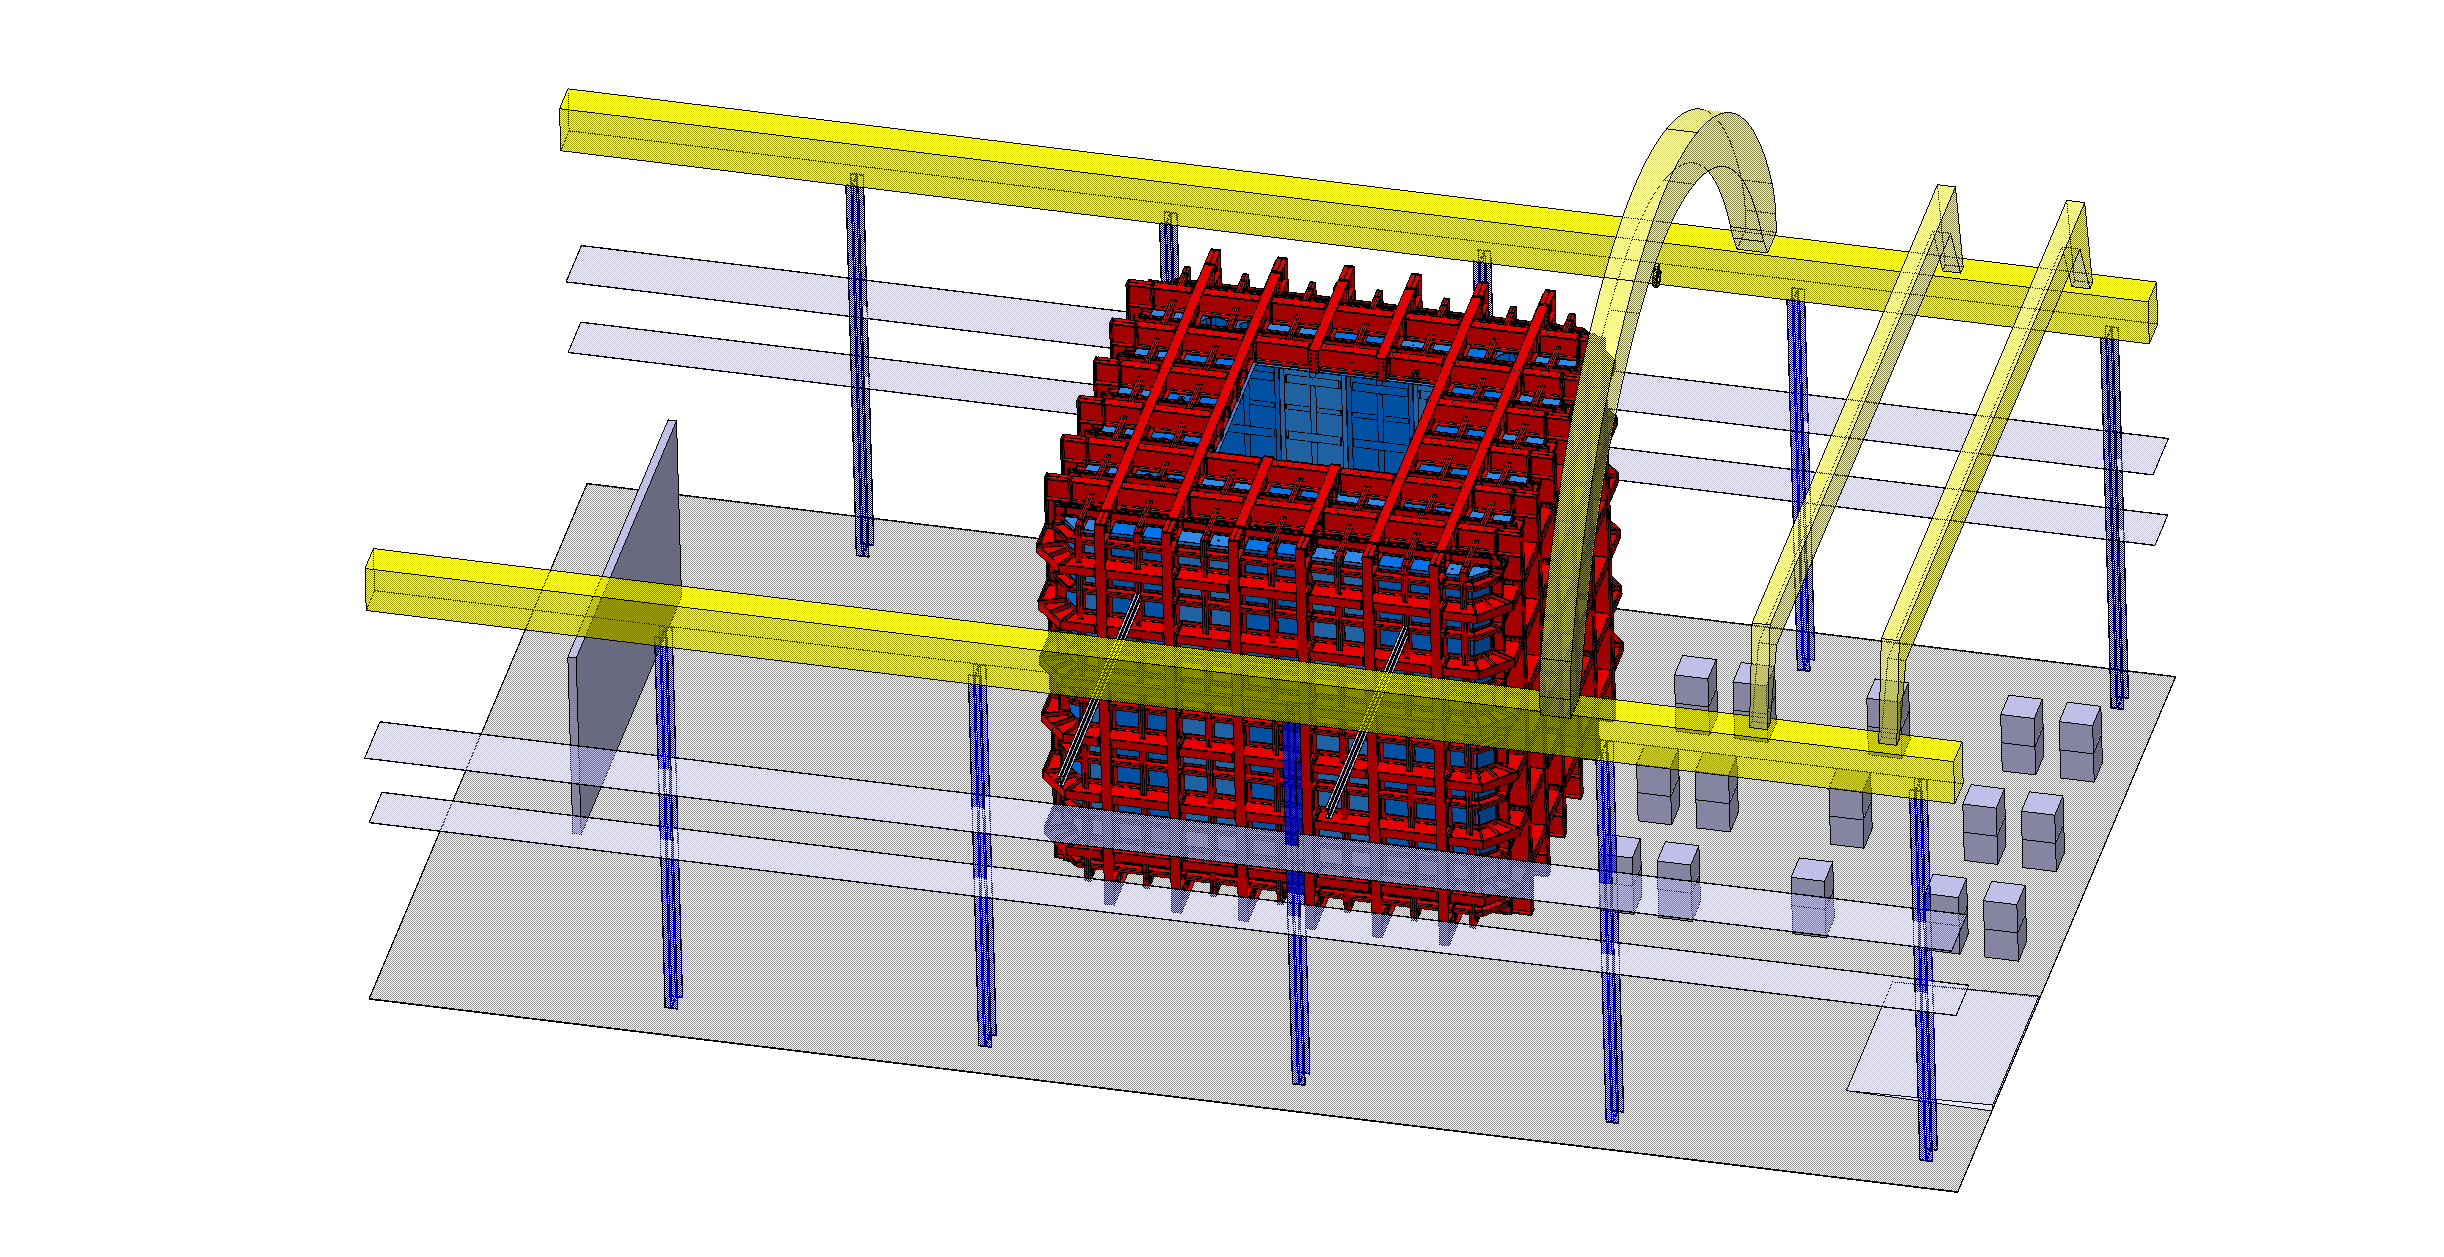
\includegraphics[width=0.32\textwidth]{./Figures/assembly_sequence_11_07/42.png}}
\subfigure[]{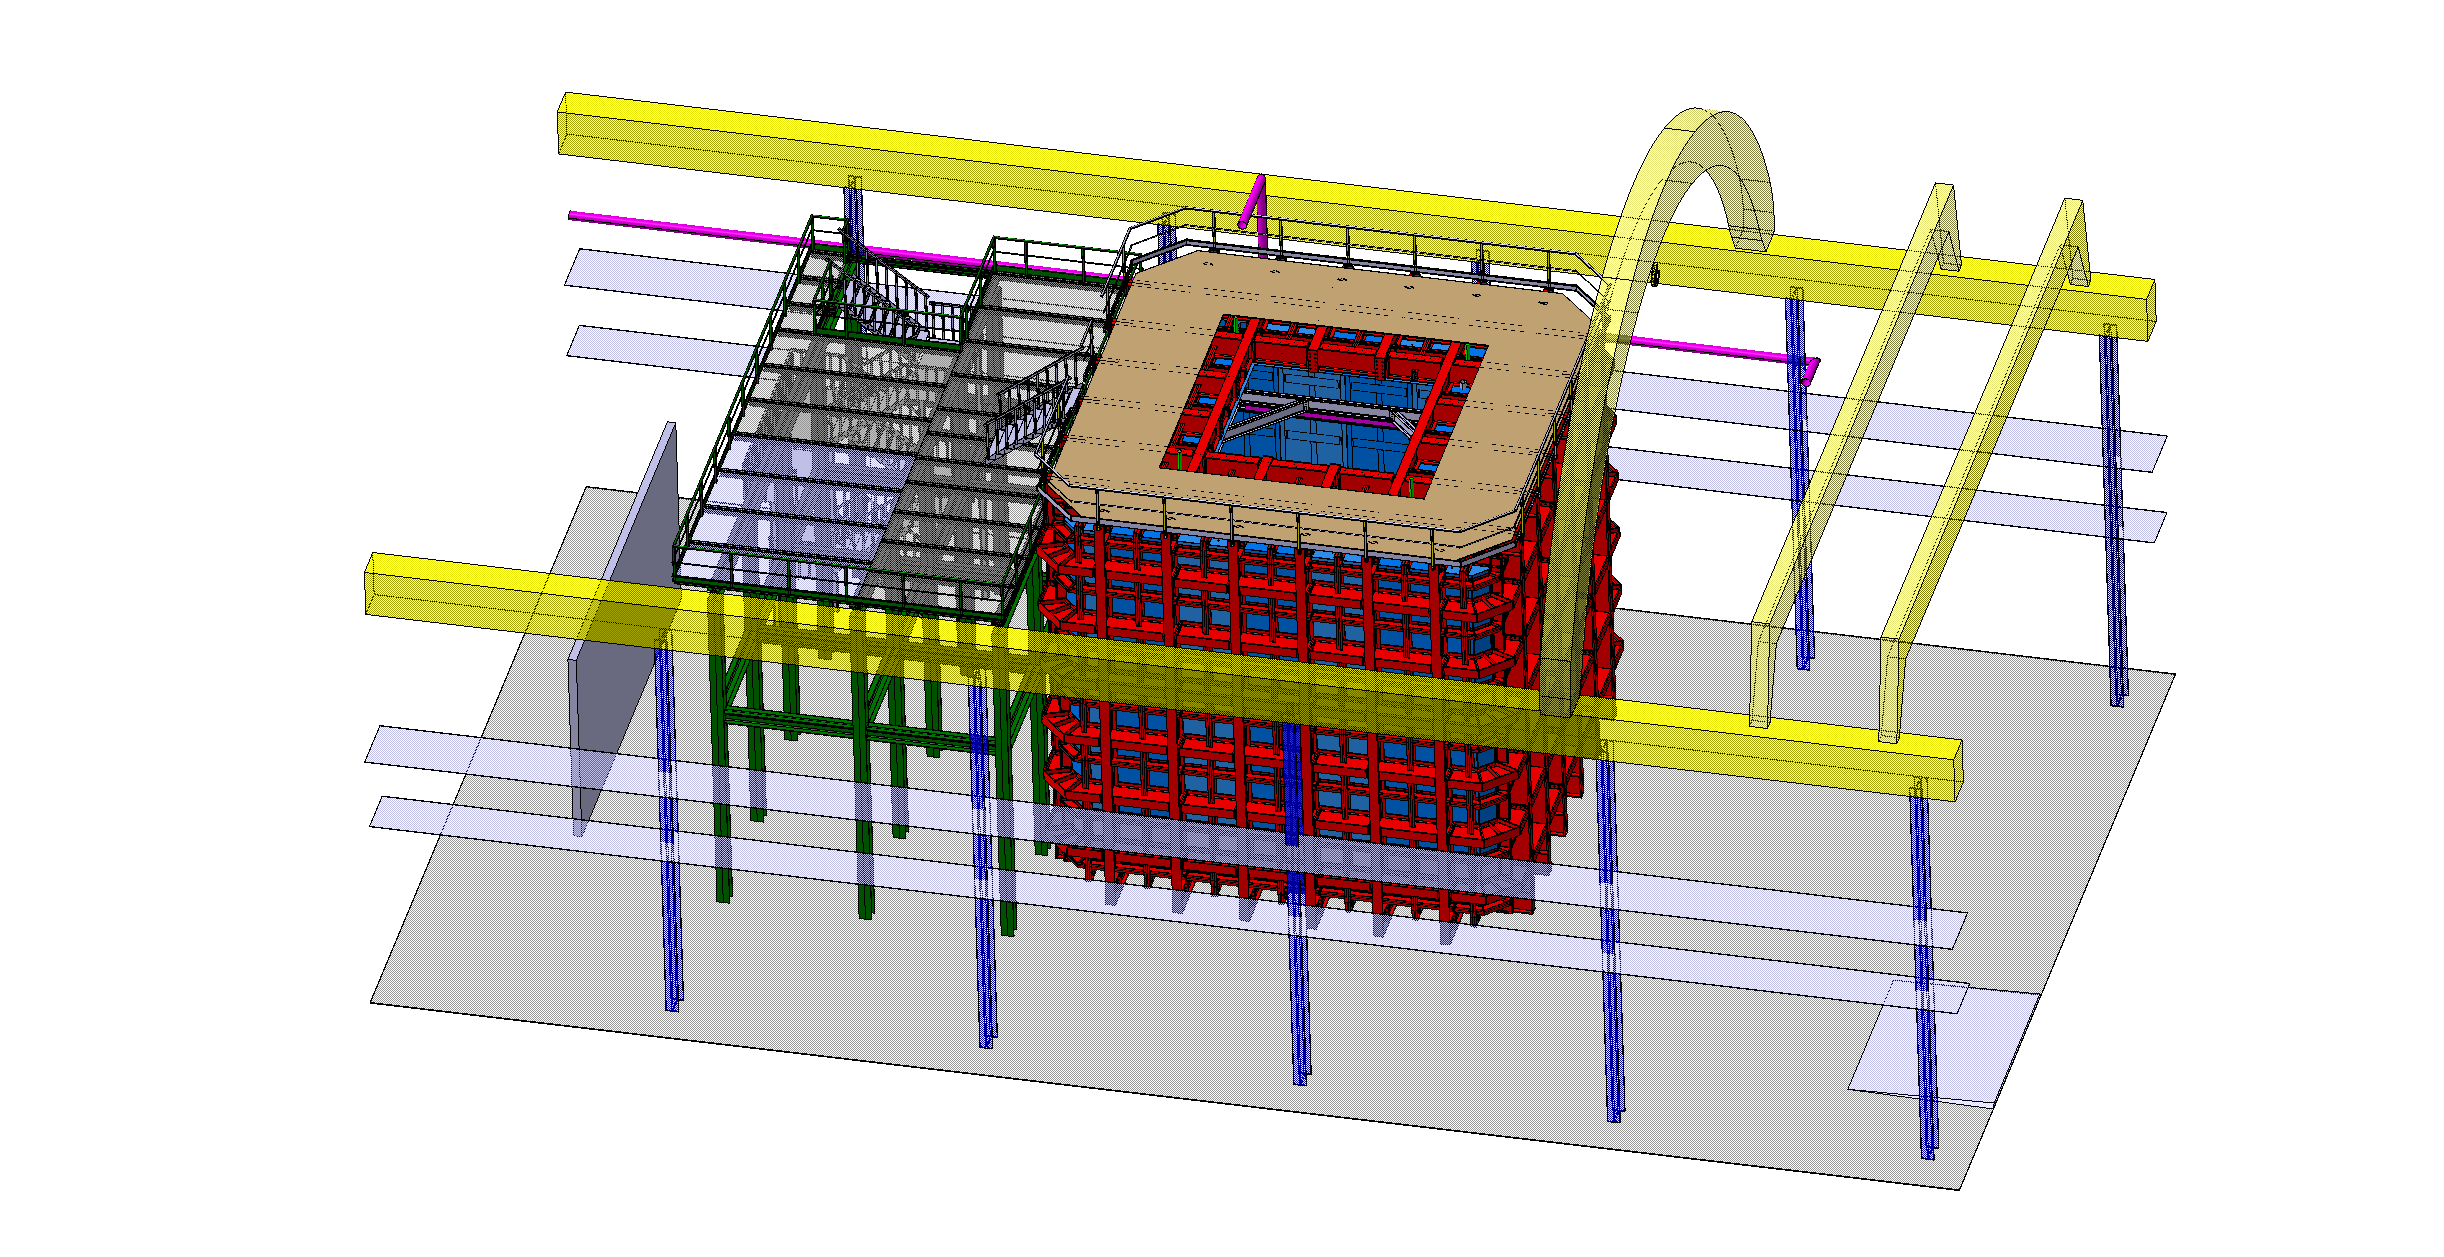
\includegraphics[width=0.32\textwidth]{./Figures/assembly_sequence_11_07/43.png}}
\subfigure[]{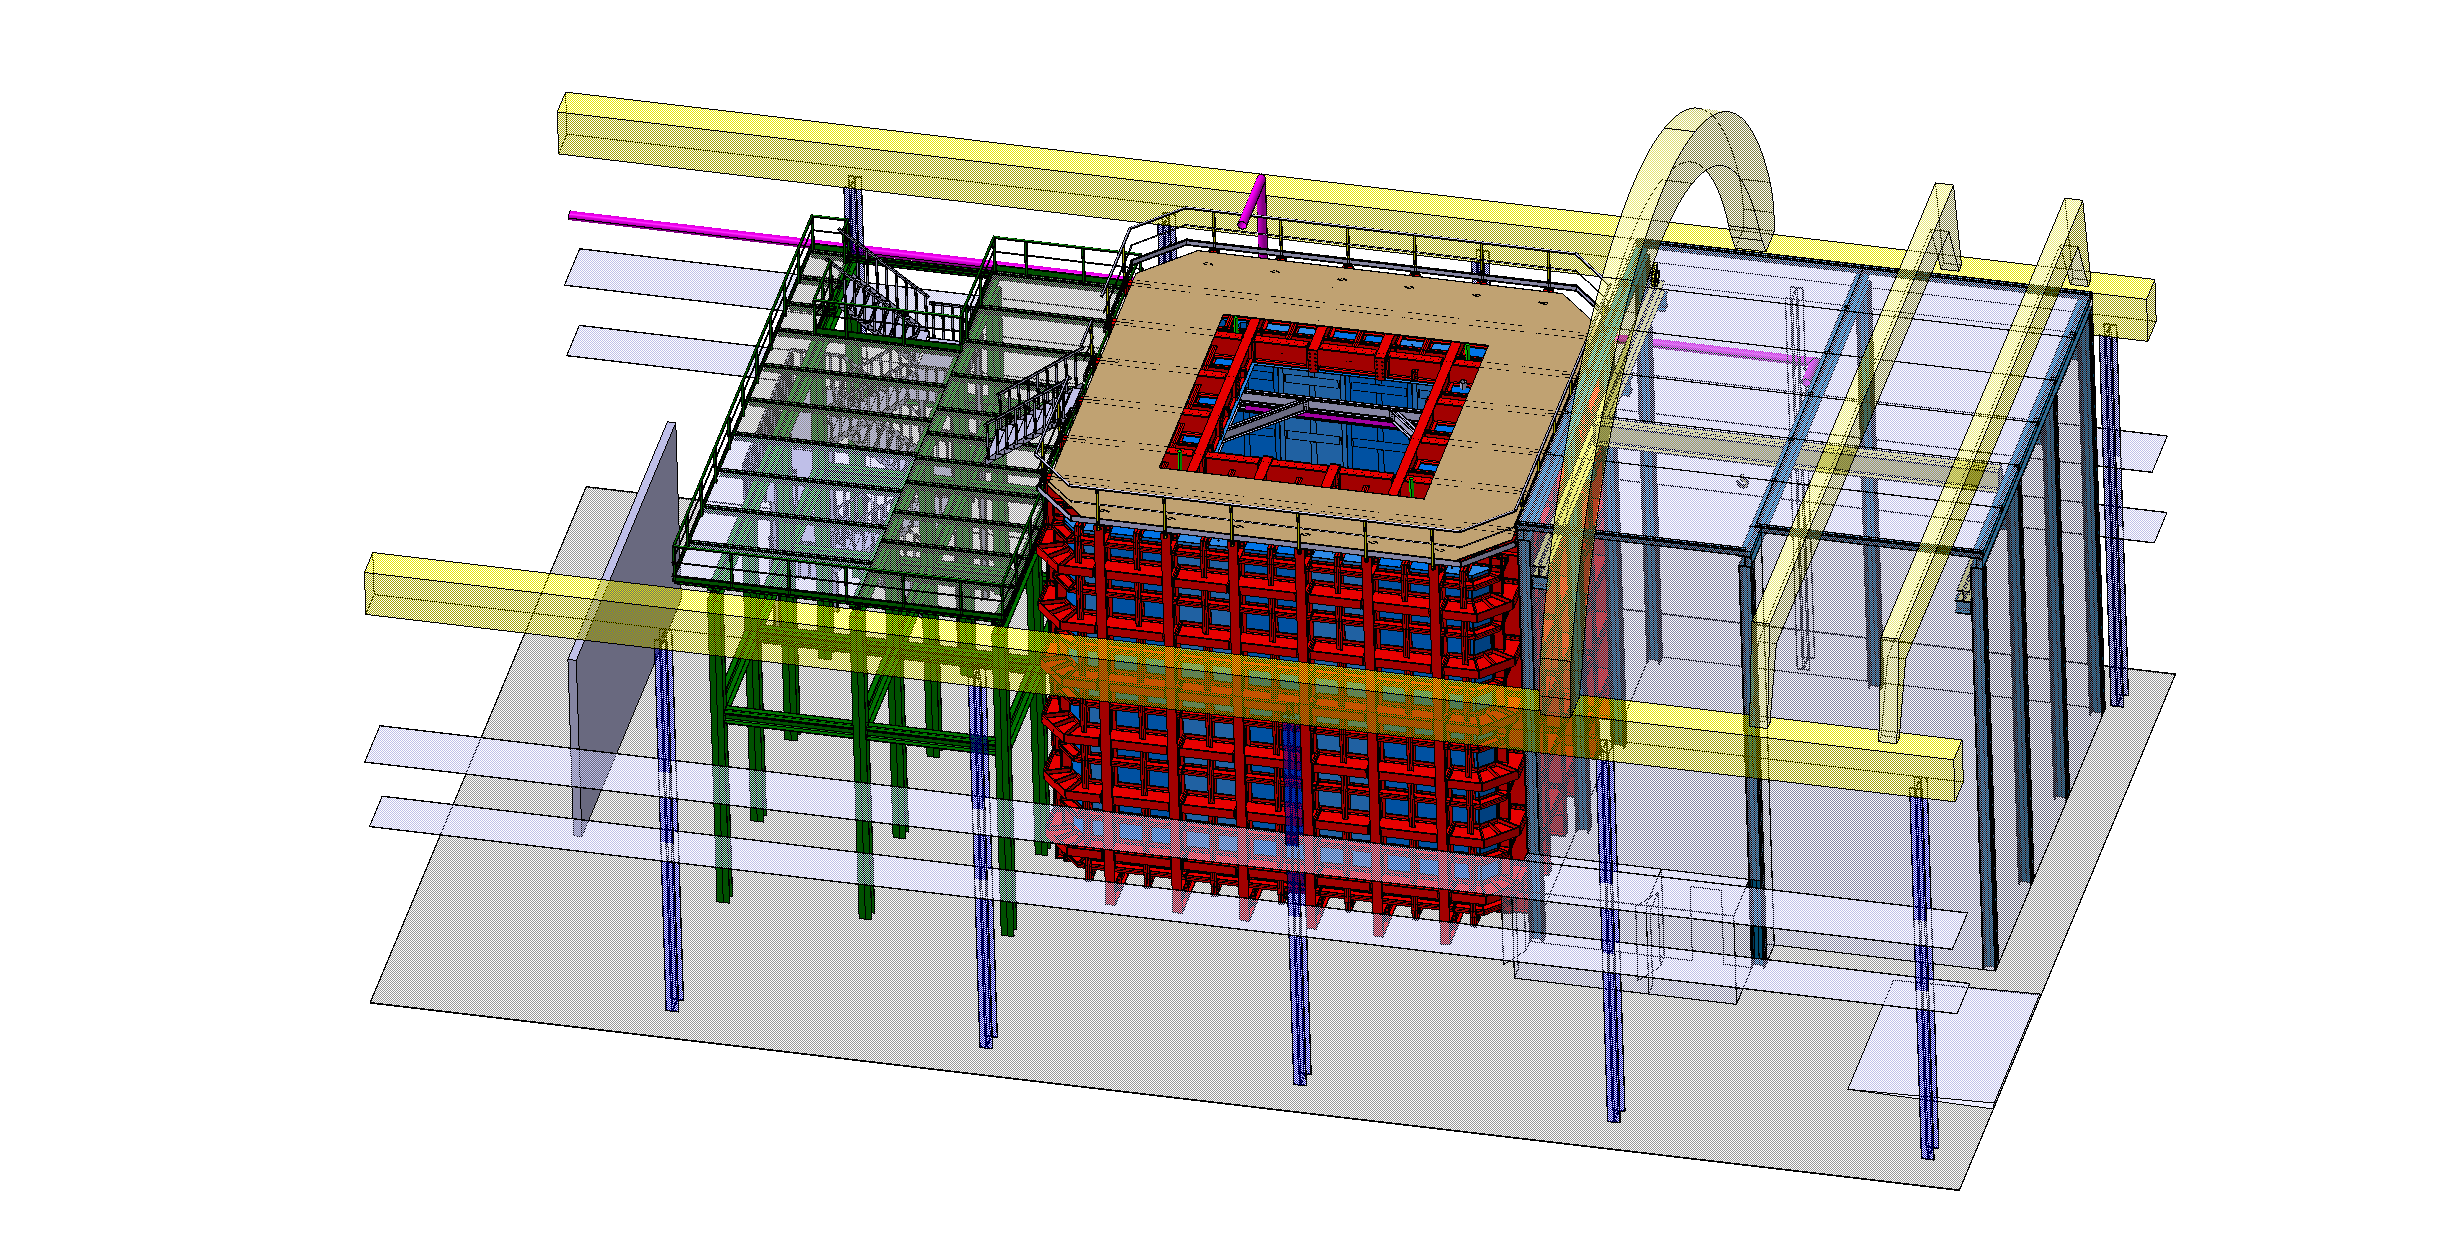
\includegraphics[width=0.32\textwidth]{./Figures/assembly_sequence_11_07/44.png}}
\subfigure[]{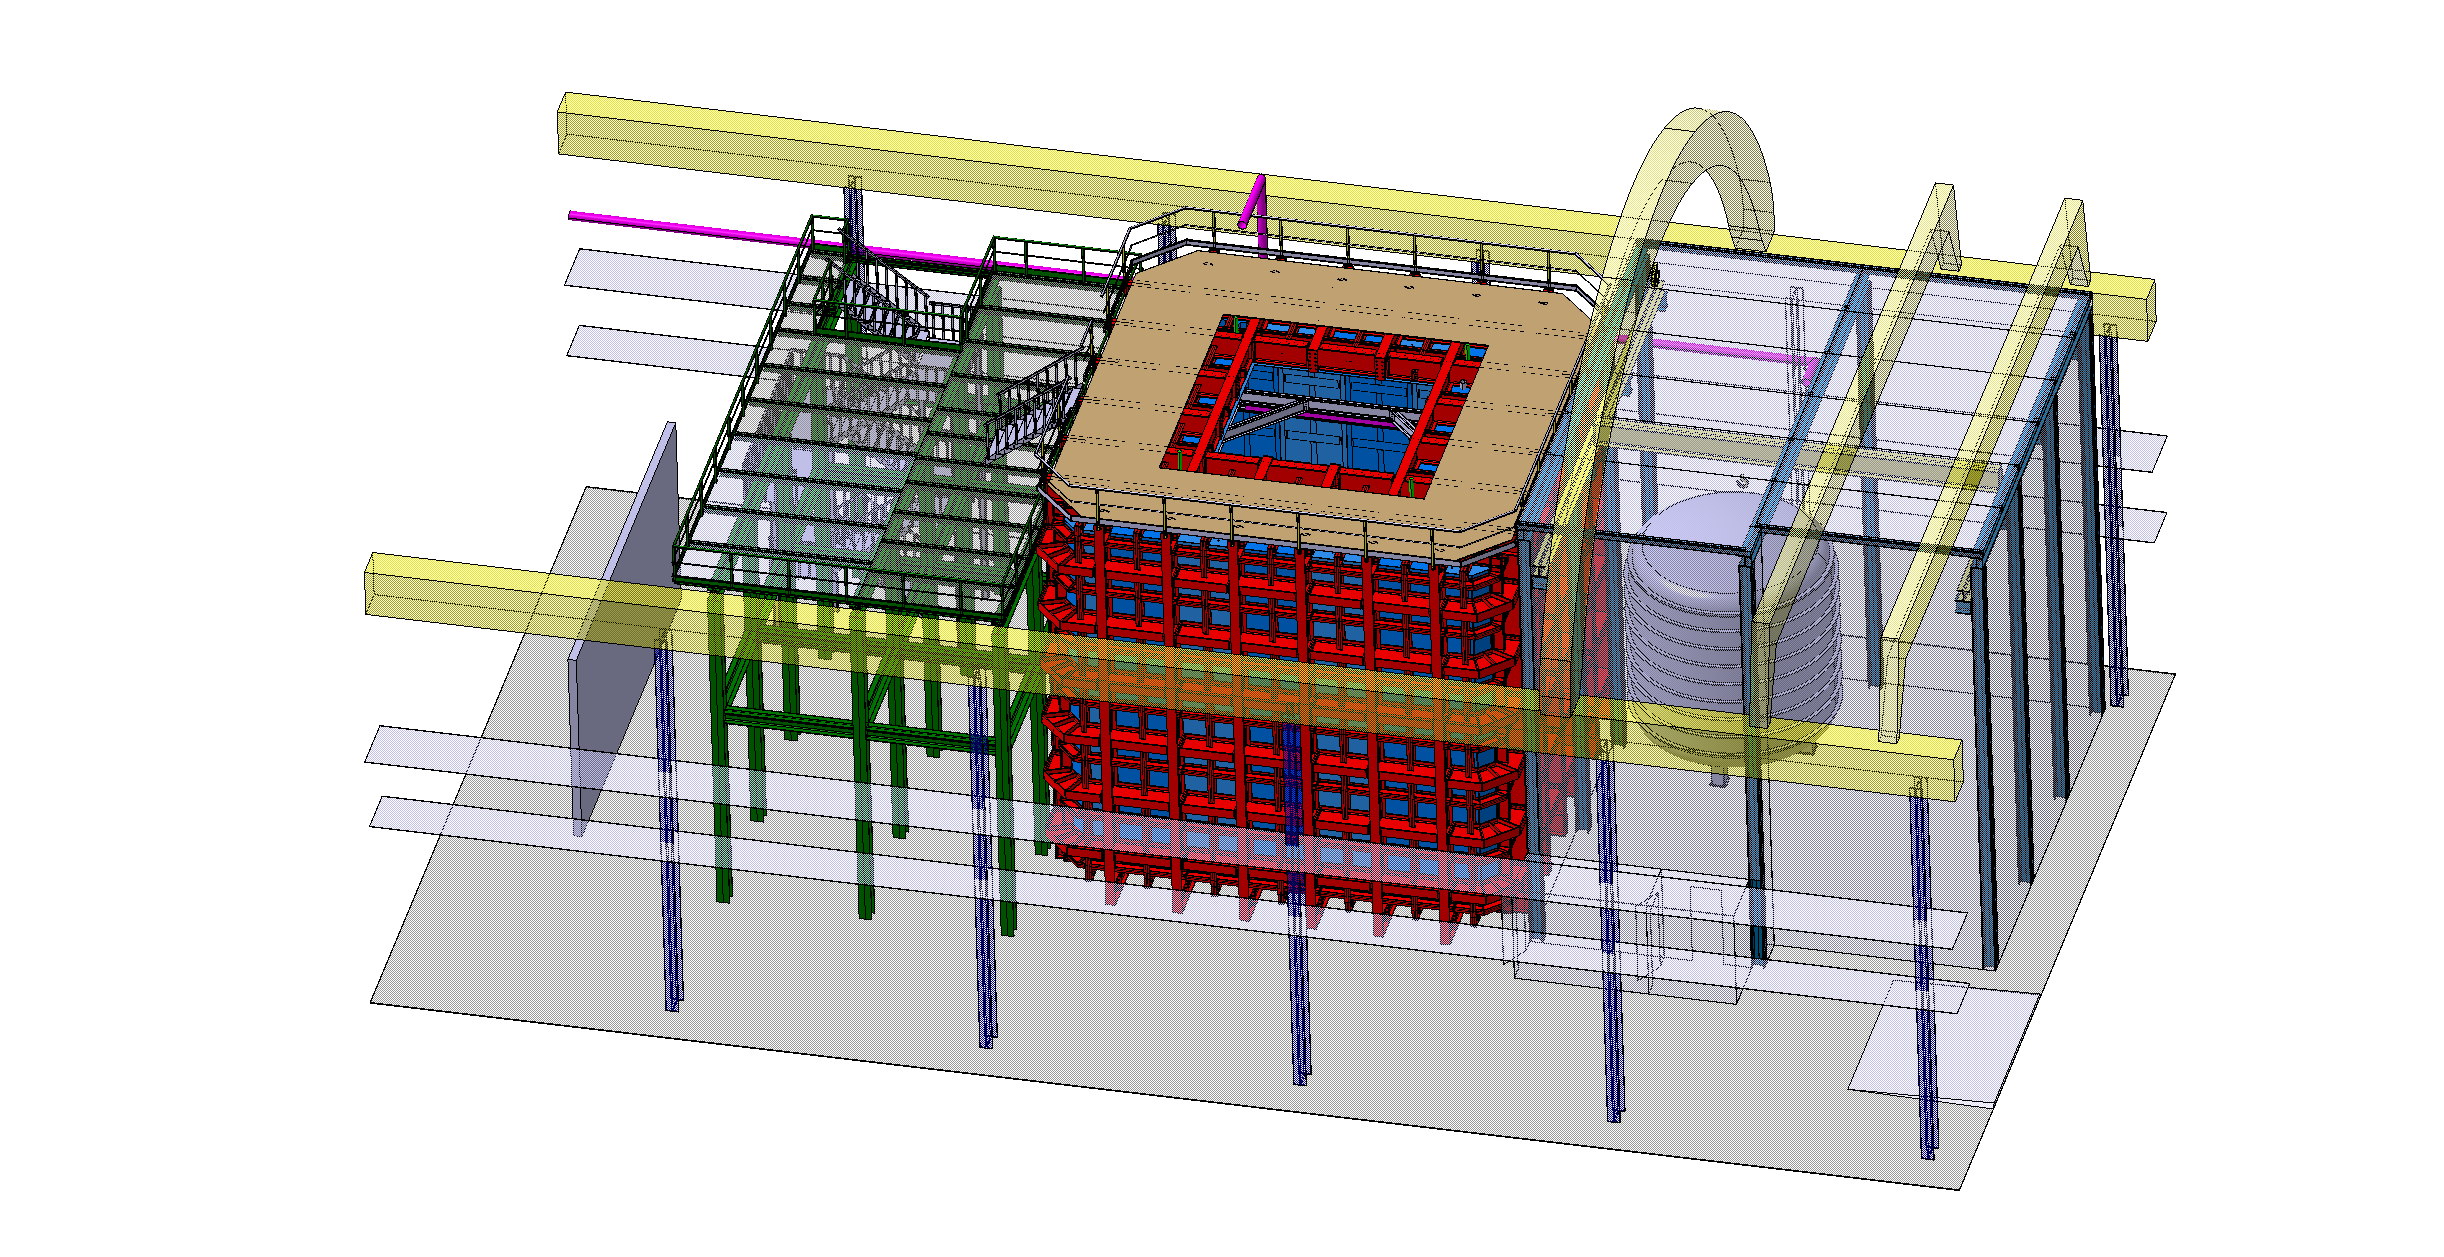
\includegraphics[width=0.32\textwidth]{./Figures/assembly_sequence_11_07/45.png}}
\subfigure[]{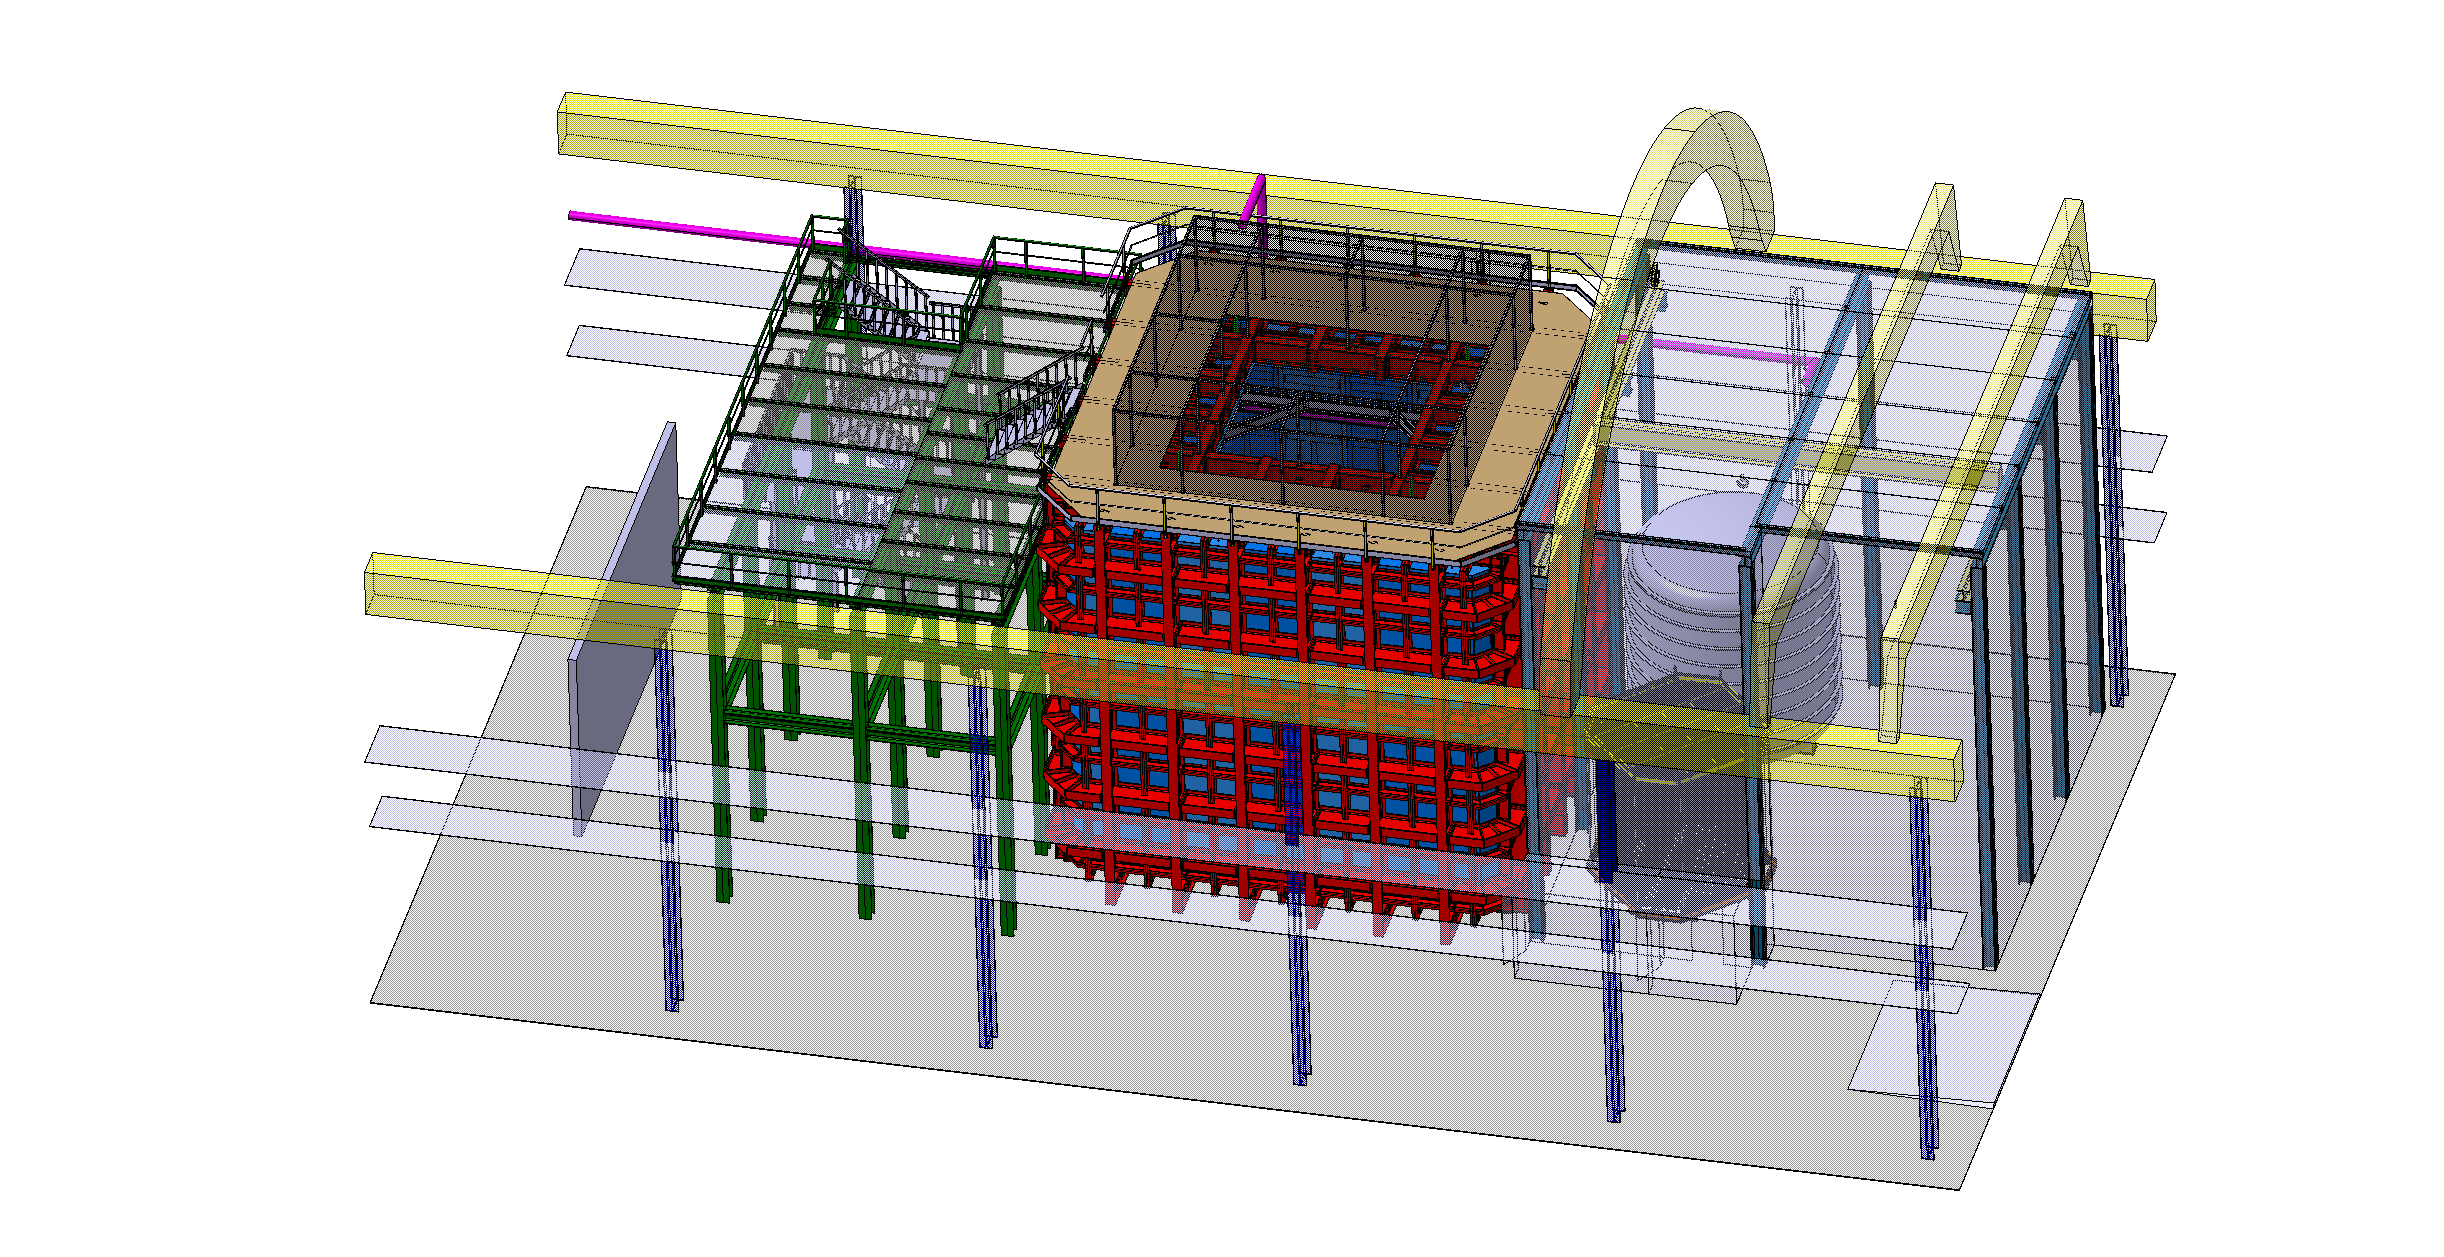
\includegraphics[width=0.32\textwidth]{./Figures/assembly_sequence_11_07/46.png}}
\subfigure[]{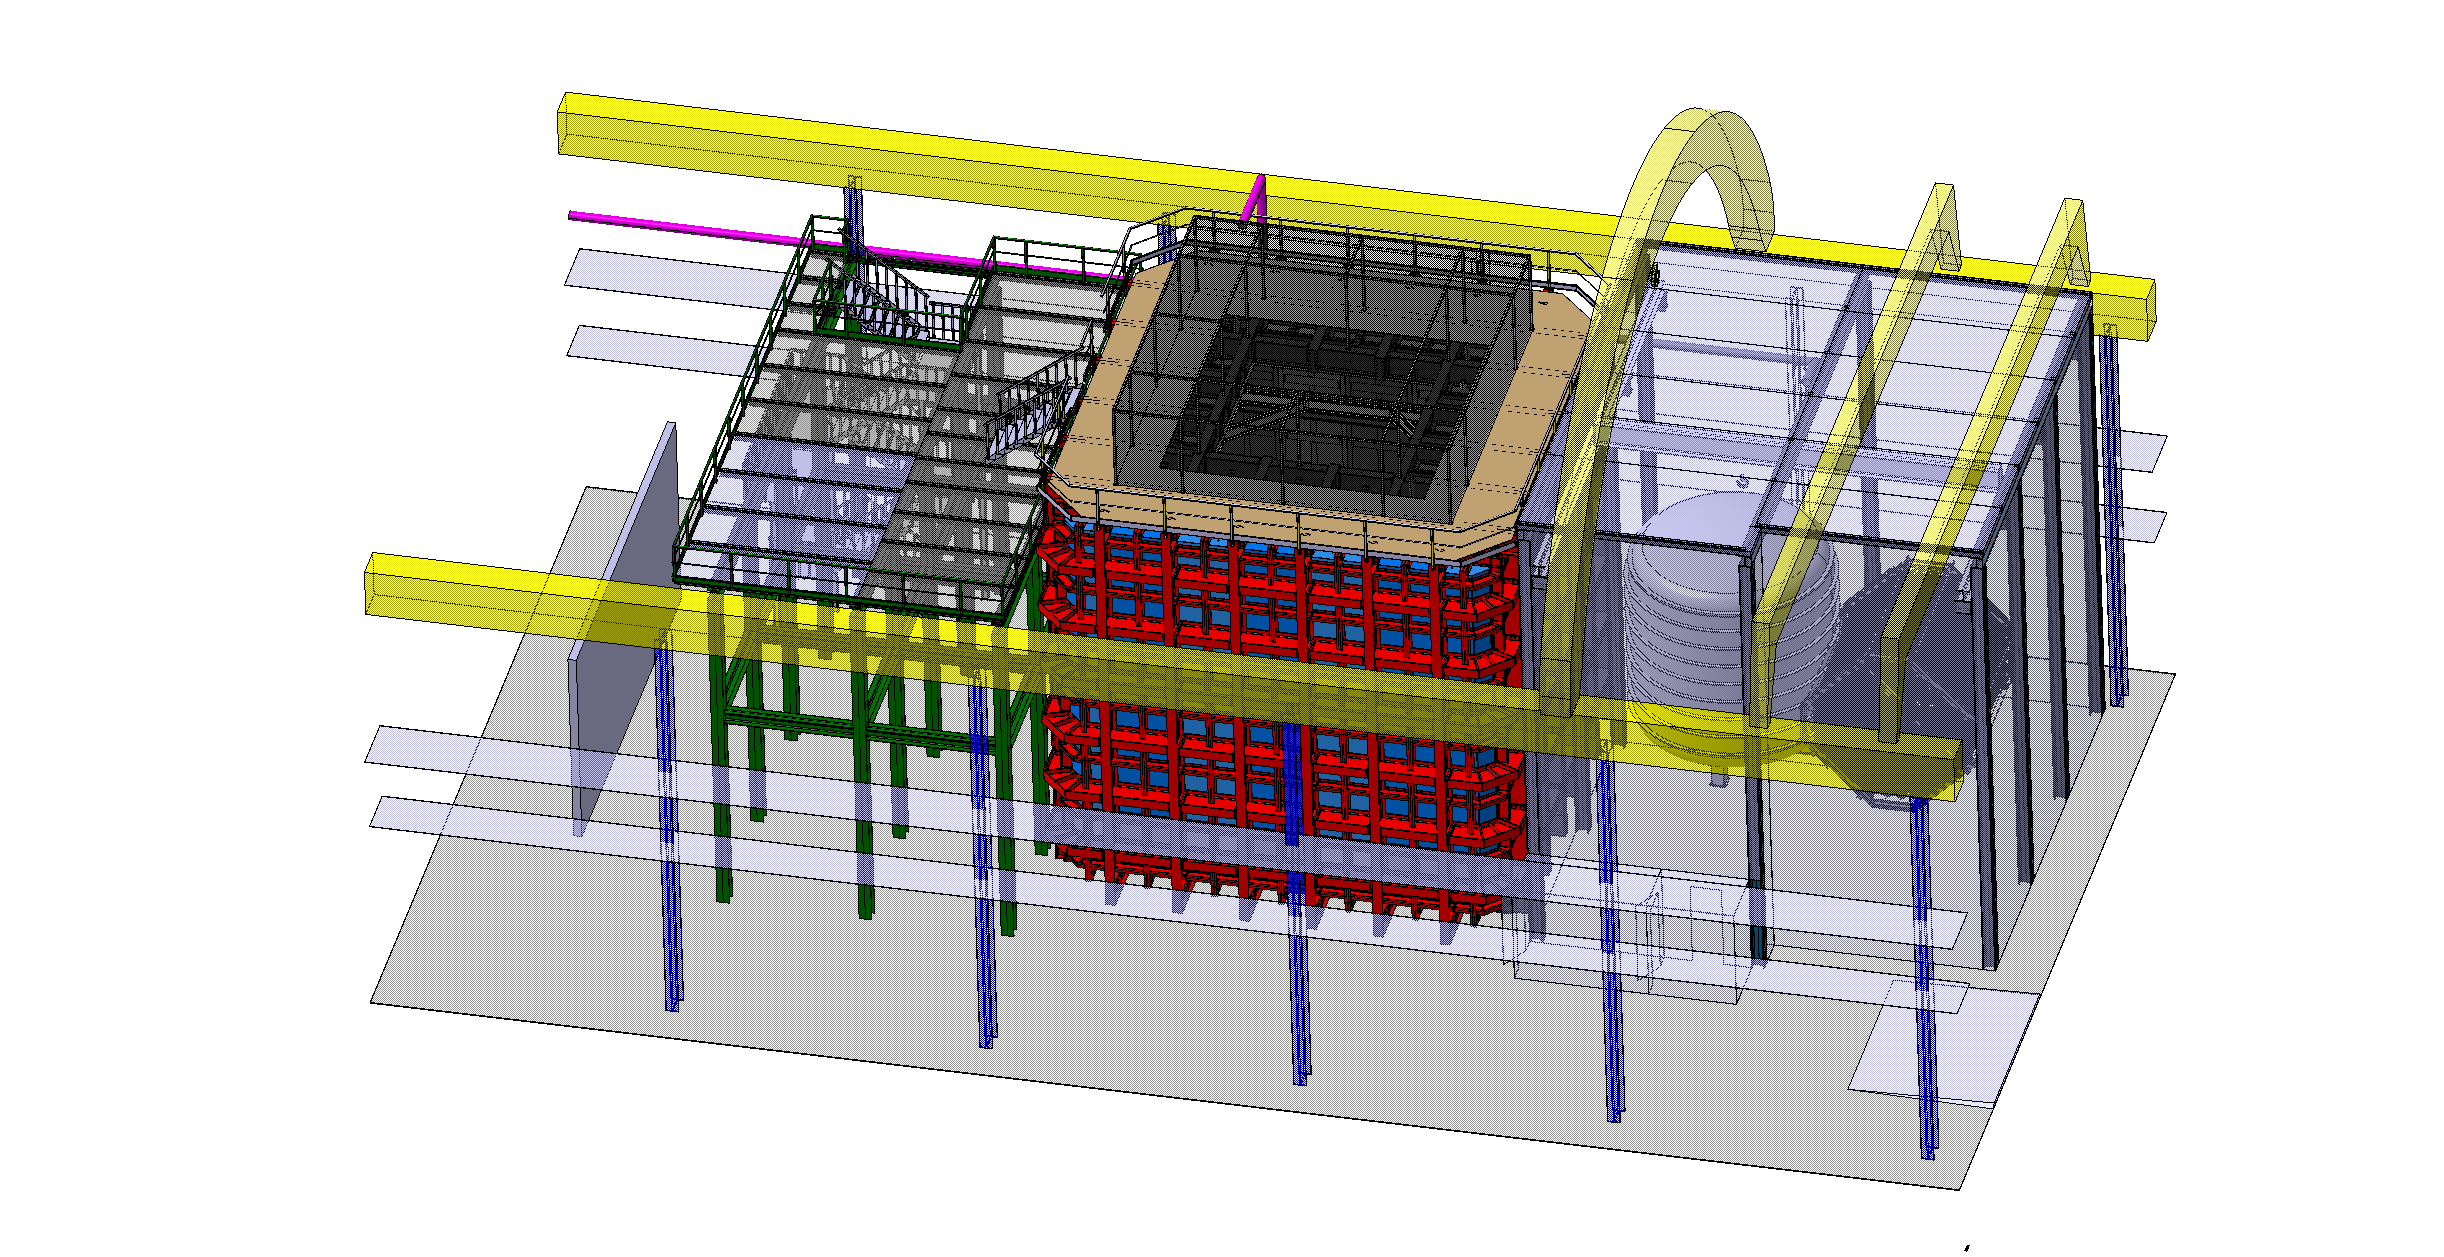
\includegraphics[width=0.32\textwidth]{./Figures/assembly_sequence_11_07/47.png}}
\subfigure[]{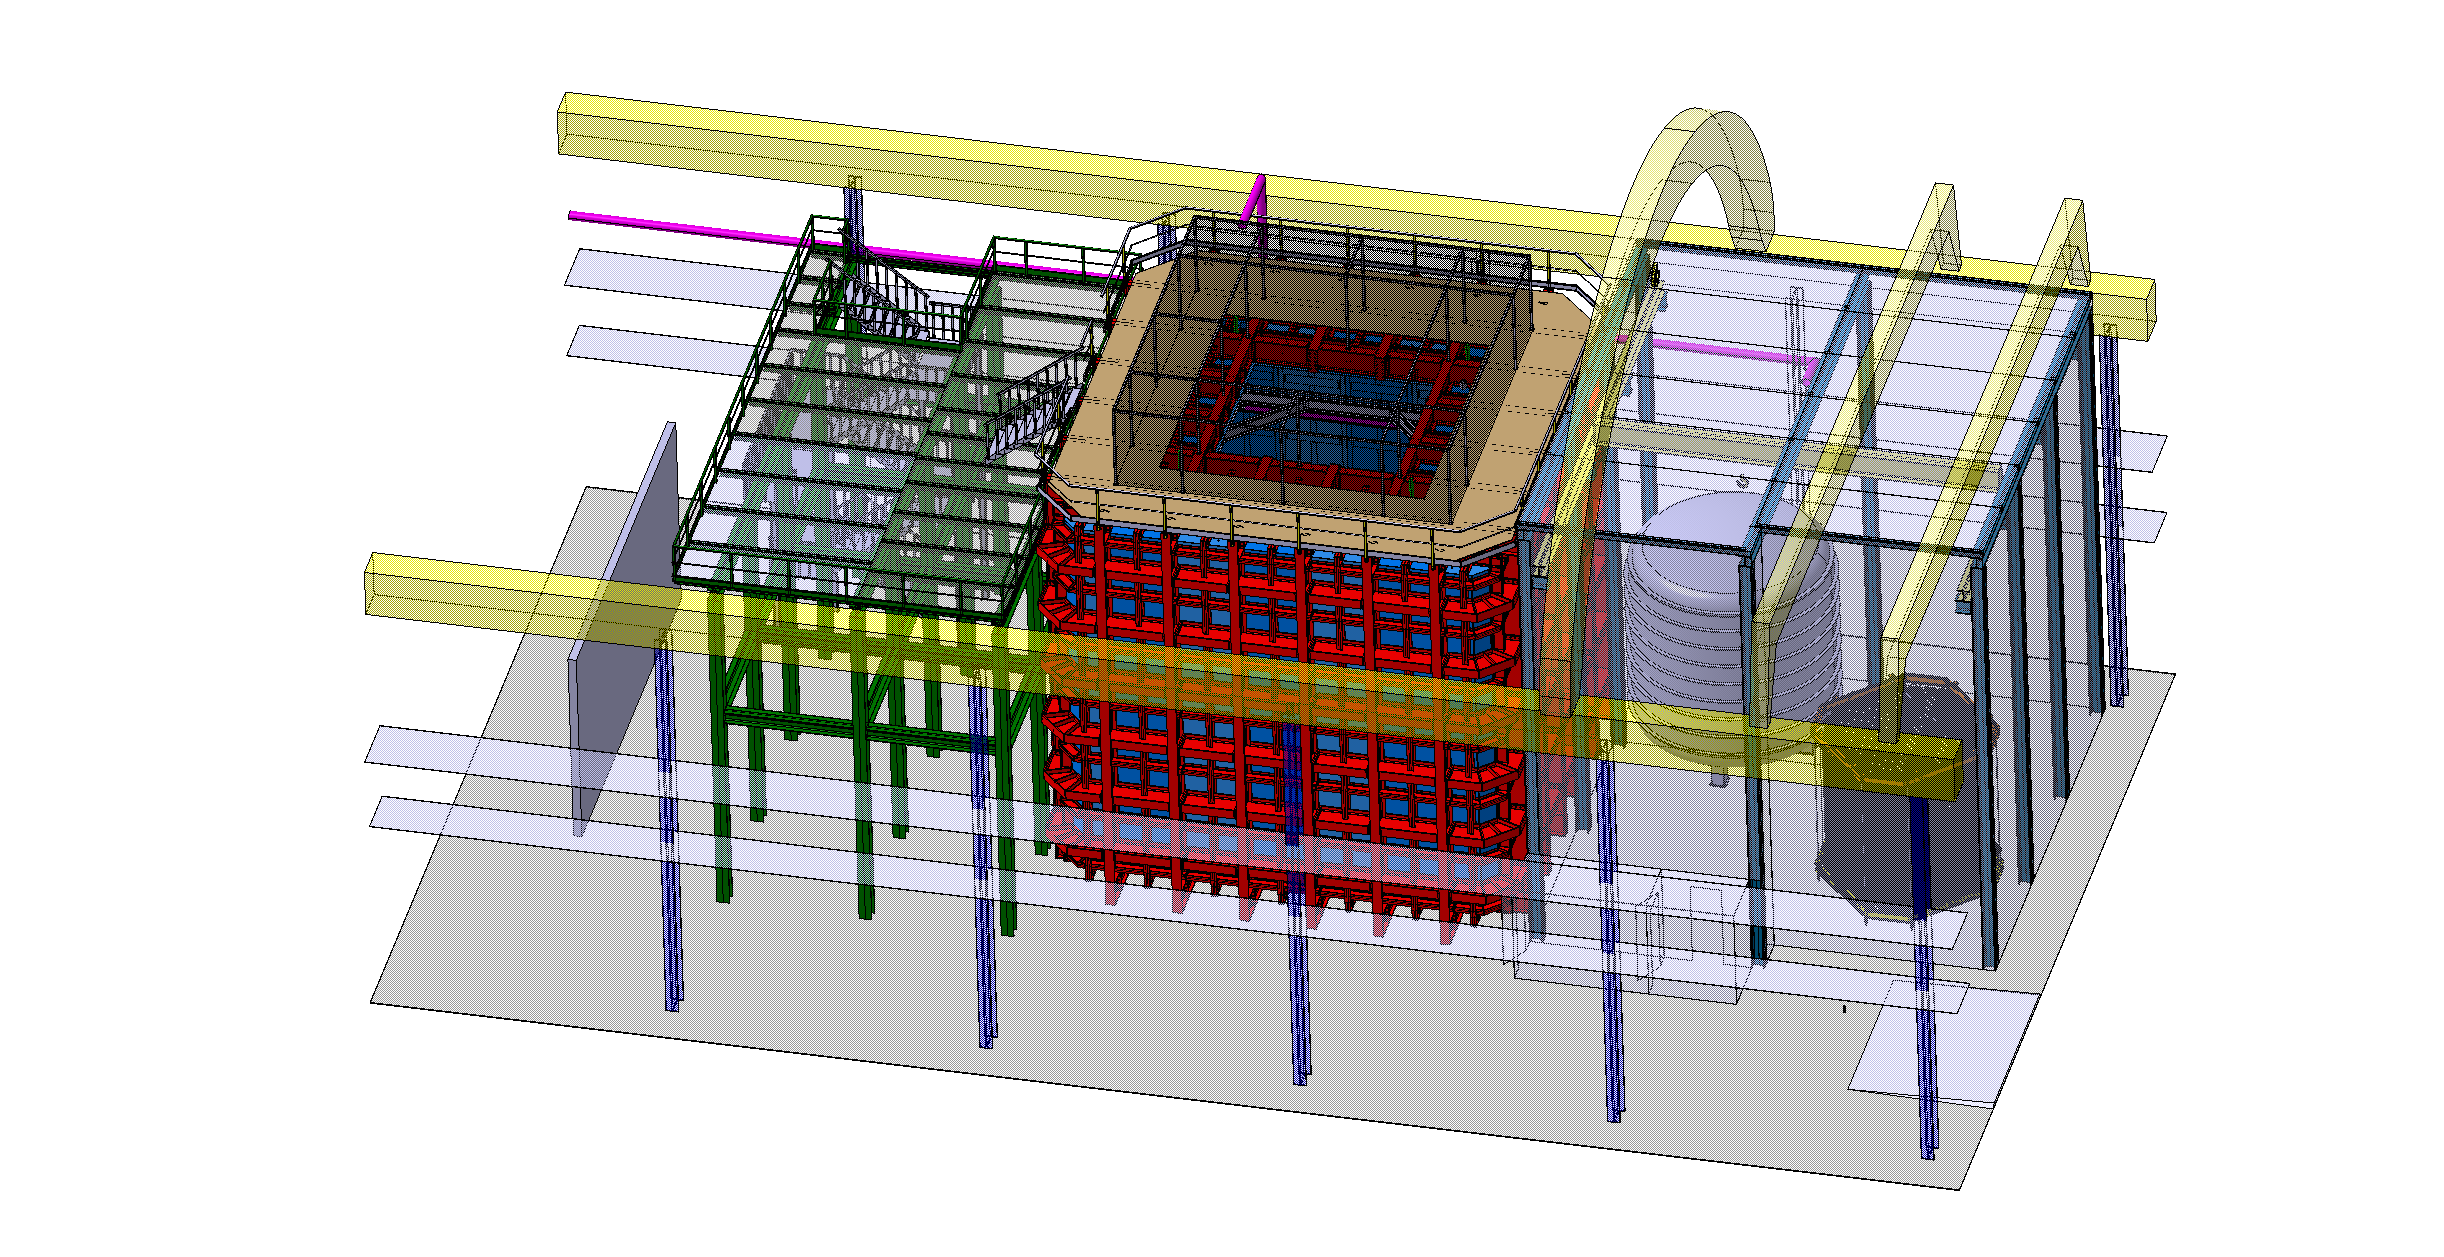
\includegraphics[width=0.32\textwidth]{./Figures/assembly_sequence_11_07/48.png}}
\subfigure[]{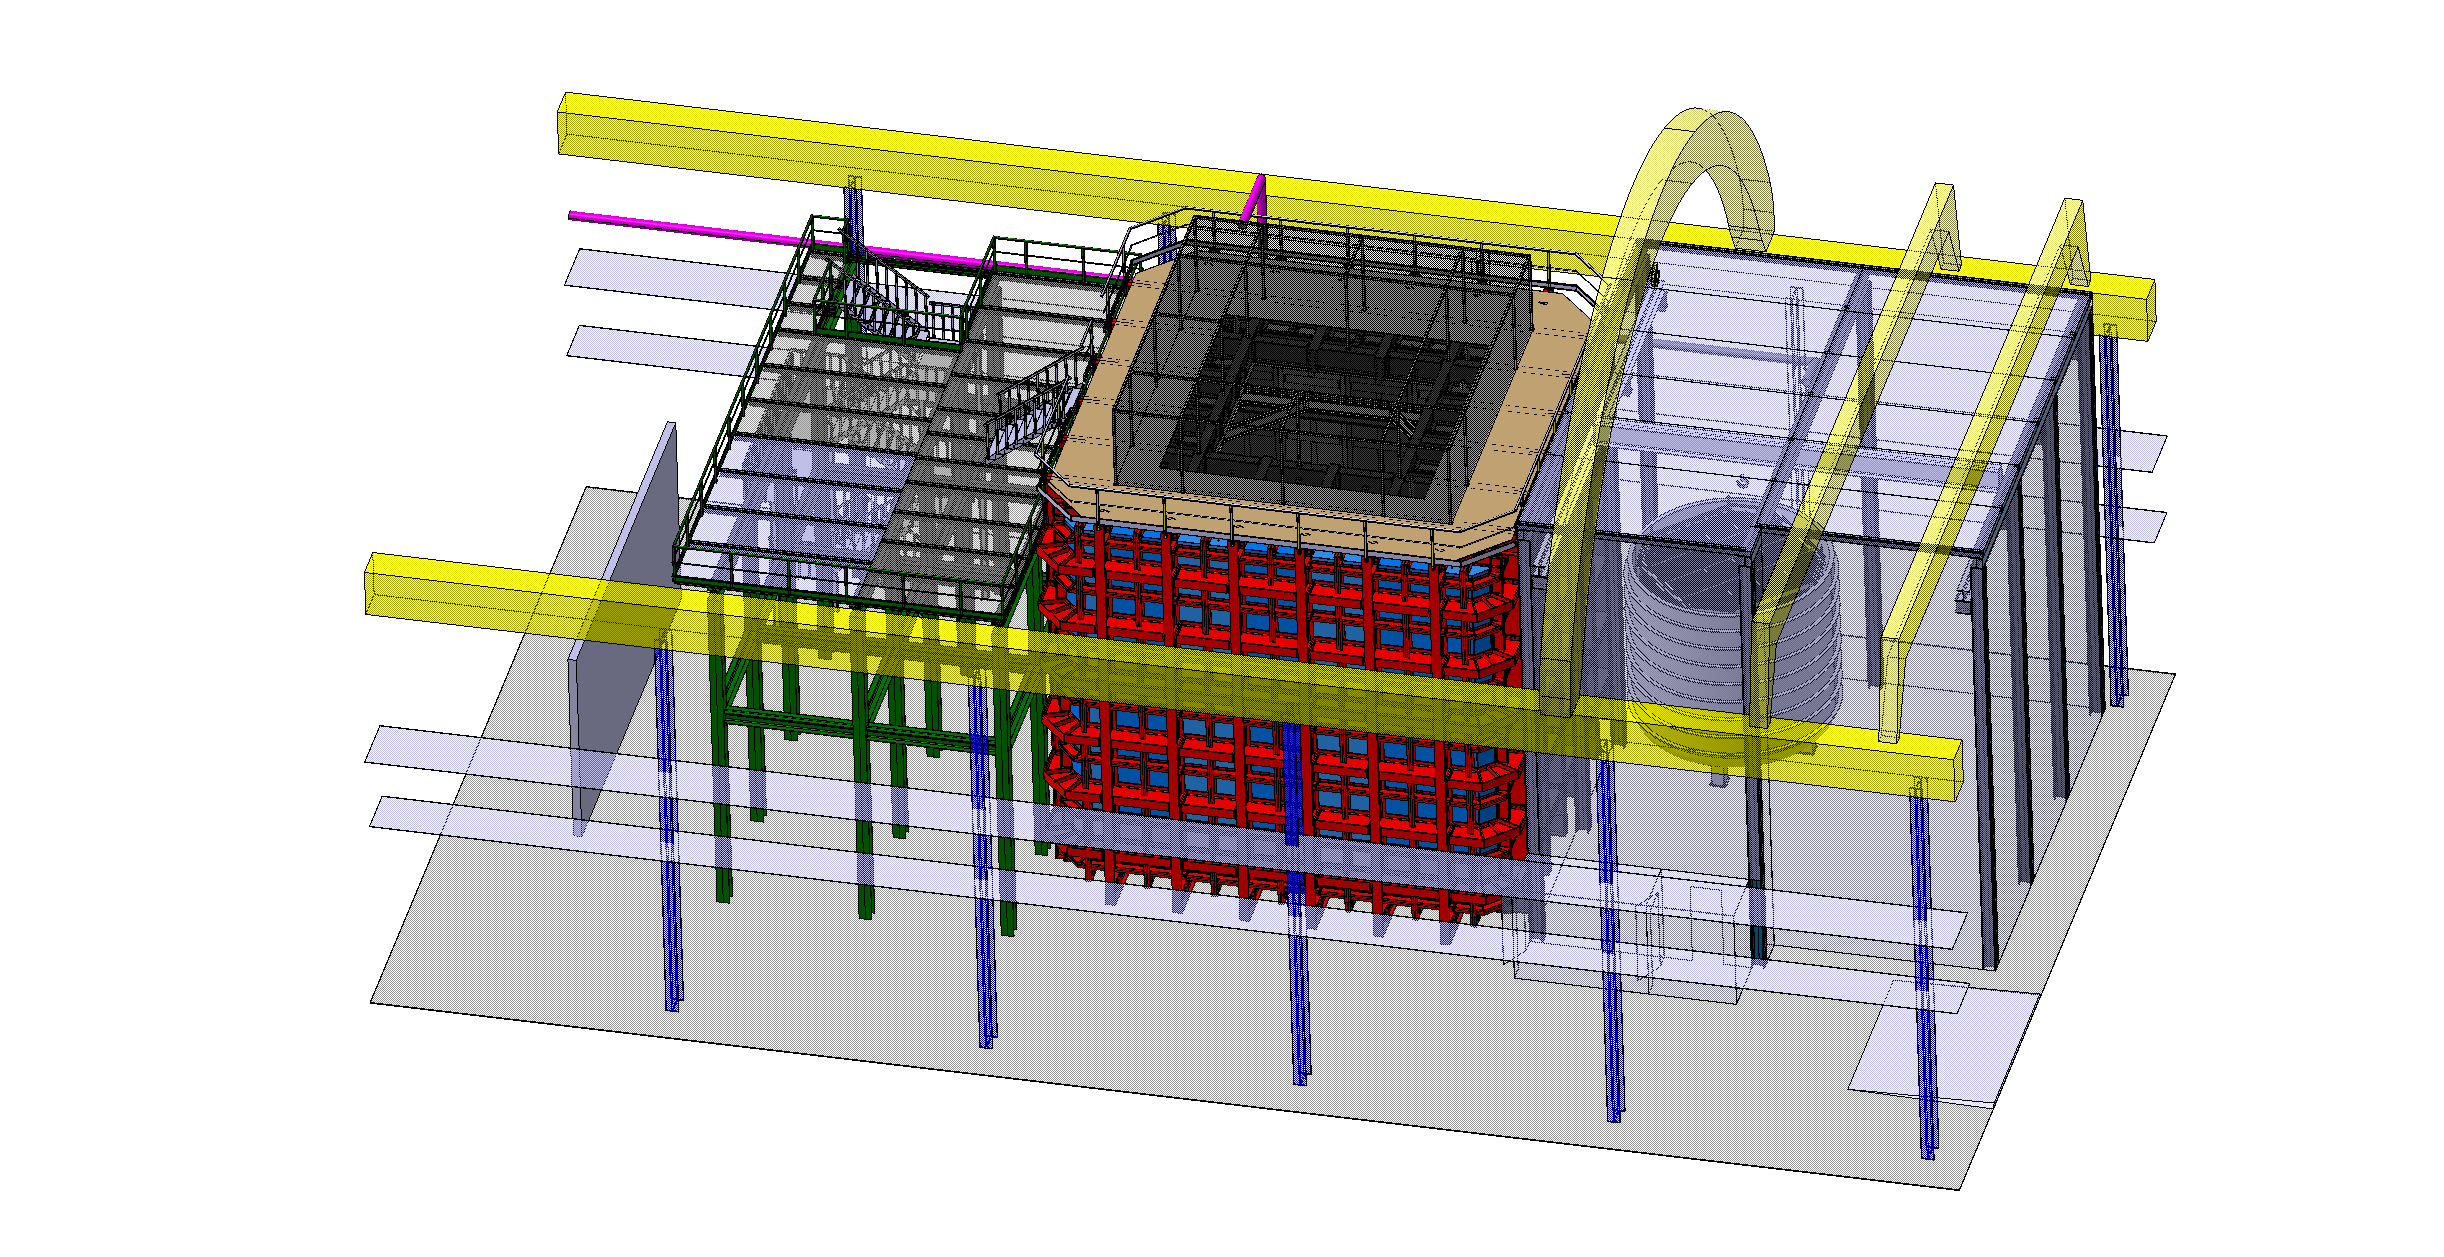
\includegraphics[width=0.32\textwidth]{./Figures/assembly_sequence_11_07/49.png}}
\subfigure[]{\includegraphics[width=0.32\textwidth]{./Figures/assembly_sequence_11_07/50.png}}
\subfigure[]{\includegraphics[width=0.32\textwidth]{./Figures/assembly_sequence_11_07/51.png}}
\subfigure[]{\includegraphics[width=0.32\textwidth]{./Figures/assembly_sequence_11_07/52.png}}
\subfigure[]{\includegraphics[width=0.32\textwidth]{./Figures/assembly_sequence_11_07/53.png}}
\caption{Details of the installation sequence (III) }
\label{fig:Ds20kInstallSequence3}
\end{figure*}

\begin{figure*}[!t]
\subfigure[]{\includegraphics[width=0.32\textwidth]{./Figures/assembly_sequence_11_07/54.png}}
\subfigure[]{\includegraphics[width=0.32\textwidth]{./Figures/assembly_sequence_11_07/55.png}}
\subfigure[]{\includegraphics[width=0.32\textwidth]{./Figures/assembly_sequence_11_07/56.png}}
\subfigure[]{\includegraphics[width=0.32\textwidth]{./Figures/assembly_sequence_11_07/57.png}}
\subfigure[]{\includegraphics[width=0.32\textwidth]{./Figures/assembly_sequence_11_07/58.png}}
\caption{Details of the installation sequence (IV) }
\label{fig:Ds20kInstallSequence4}
\end{figure*}

\newpage
